\documentclass[a4paper,twoside=true,openright,parskip=full,chapterprefix=true,11pt,headings=normal,bibliography=totoc,listof=totoc,titlepage=on,captions=tableabove,draft=false]{scrreprt}
\usepackage{lmodern}
\usepackage{amssymb,amsmath}
\usepackage{ifxetex,ifluatex}
\usepackage{fixltx2e} % provides \textsubscript
\ifnum 0\ifxetex 1\fi\ifluatex 1\fi=0 % if pdftex
  \usepackage[T1]{fontenc}
  \usepackage[utf8]{inputenc}
\else % if luatex or xelatex
  \ifxetex
    \usepackage{mathspec}
  \else
    \usepackage{fontspec}
  \fi
  \defaultfontfeatures{Ligatures=TeX,Scale=MatchLowercase}
\fi
% use upquote if available, for straight quotes in verbatim environments
\IfFileExists{upquote.sty}{\usepackage{upquote}}{}
% use microtype if available
\IfFileExists{microtype.sty}{%
\usepackage[]{microtype}
\UseMicrotypeSet[protrusion]{basicmath} % disable protrusion for tt fonts
}{}
\PassOptionsToPackage{hyphens}{url} % url is loaded by hyperref
\usepackage[unicode=true]{hyperref}
\hypersetup{
            pdftitle={Genome folding in evolution and disease},
            pdfauthor={Jonas Ibn-Salem},
            pdfborder={0 0 0},
            breaklinks=true}
\urlstyle{same}  % don't use monospace font for urls
\usepackage{natbib}
\bibliographystyle{unsrtnat}
\usepackage{longtable,booktabs}
% Fix footnotes in tables (requires footnote package)
\IfFileExists{footnote.sty}{\usepackage{footnote}\makesavenoteenv{long table}}{}
\IfFileExists{parskip.sty}{%
\usepackage{parskip}
}{% else
\setlength{\parindent}{0pt}
\setlength{\parskip}{6pt plus 2pt minus 1pt}
}
\setlength{\emergencystretch}{3em}  % prevent overfull lines
\providecommand{\tightlist}{%
  \setlength{\itemsep}{0pt}\setlength{\parskip}{0pt}}
\setcounter{secnumdepth}{5}
% Redefines (sub)paragraphs to behave more like sections
\ifx\paragraph\undefined\else
\let\oldparagraph\paragraph
\renewcommand{\paragraph}[1]{\oldparagraph{#1}\mbox{}}
\fi
\ifx\subparagraph\undefined\else
\let\oldsubparagraph\subparagraph
\renewcommand{\subparagraph}[1]{\oldsubparagraph{#1}\mbox{}}
\fi

% set default figure placement to htbp
\makeatletter
\def\fps@figure{htbp}
\makeatother

\usepackage{booktabs}
\usepackage{amsthm}


%%%%%%%%%%%%%%%%%%%%%%%%%%%%%%%%%%%%%%%%%%%%%%%%%%%%%%%%%%%%%%%%%%%%%%%%%%%%%%%%
% Code from cleanthesis
%%%%%%%%%%%%%%%%%%%%%%%%%%%%%%%%%%%%%%%%%%%%%%%%%%%%%%%%%%%%%%%%%%%%%%%%%%%%%%%%



% **************************************************
% Files' Character Encoding
% **************************************************
\PassOptionsToPackage{utf8}{inputenc}
\usepackage{inputenc}


% **************************************************
% Information and Commands for Reuse
% **************************************************
\newcommand{\thesisTitle}{Genome folding in evolution and disease}
\newcommand{\thesisName}{Jonas Ibn-Salem}
\newcommand{\thesisSubject}{Documentation}
% \newcommand{\thesisDate}{January, 2018}
\newcommand{\thesisDate}{\today}
\newcommand{\thesisVersion}{0.0.1}

\newcommand{\thesisFirstReviewer}{Prof. Dr. Miguel Andrade-Navarro}
\newcommand{\thesisFirstReviewerUniversity}{\protect{Johannes Gutenberg-Universität Mainz}}
\newcommand{\thesisFirstReviewerDepartment}{Fachbereich Biologie}

\newcommand{\thesisSecondReviewer}{Prof. Dr. Thomas Hankeln}
\newcommand{\thesisSecondReviewerUniversity}{\protect{Johannes Gutenberg-Universität Mainz}}
\newcommand{\thesisSecondReviewerDepartment}{Fachbereich Biologie}

\newcommand{\thesisFirstSupervisor}{Miguel Andrade}
\newcommand{\thesisSecondSupervisor}{}

\newcommand{\thesisUniversity}{\protect{Johannes Gutenberg-Universität Mainz}}
\newcommand{\thesisUniversityDepartment}{Fachbereich Biologie}
\newcommand{\thesisUniversityInstitute}{Institute of Organismic and Molecular Evolution}
\newcommand{\thesisUniversityGroup}{Computational Biology and Data Mining Group}
\newcommand{\thesisUniversityCity}{Mainz}
\newcommand{\thesisUniversityStreetAddress}{Ackermannweg 4}
\newcommand{\thesisUniversityPostalCode}{55128}


% **************************************************
% Debug LaTeX Information
% **************************************************
%\listfiles


% **************************************************
% Load and Configure Packages
% **************************************************
\usepackage[english]{babel} % babel system, adjust the language of the content
\PassOptionsToPackage{% setup clean thesis style
    figuresep=colon,%
    sansserif=false,%
    hangfigurecaption=false,%
    hangsection=true,%
    hangsubsection=true,%
    colorize=full,%
    colortheme=jgured,%
    % bibsys=bibtex,%
    % bibfile=bib-refs,%
    % bibstyle=numeric,%
    wrapfooter=false,%
}{cleanthesis}
\usepackage{cleanthesis}

\hypersetup{% setup the hyperref-package options
    pdftitle={\thesisTitle},    %   - title (PDF meta)
    pdfsubject={\thesisSubject},%   - subject (PDF meta)
    pdfauthor={\thesisName},    %   - author (PDF meta)
    plainpages=false,           %   -
    colorlinks=false,           %   - colorize links?
    linkcolor=ctcolormain,      %   - link color (e.g., TOC)
    citecolor=ctcolormain,      %   - cite color
    pdfborder={0 0 0},          %   -
    breaklinks=true,            %   - allow line break inside links
    bookmarksnumbered=true,     %
    bookmarksopen=true          %
}

\makeatletter
\def\thm@space@setup{%
  \thm@preskip=8pt plus 2pt minus 4pt
  \thm@postskip=\thm@preskip
}
\makeatother
%%%%%%%%%%%%%%%%%%%%%%%%%%%%%%%%%%%%%%%%%%%%%%%%%%%%%%%%%%%%%%%%%%%%%%%%%%%%%%%%
% Code for custome style
%%%%%%%%%%%%%%%%%%%%%%%%%%%%%%%%%%%%%%%%%%%%%%%%%%%%%%%%%%%%%%%%%%%%%%%%%%%%%%%%

% \usepackage{cell} % use cell journal style
% \usepackage[backend=bibtex]{biblatex}

\title{Genome folding in evolution and disease}
\author{Jonas Ibn-Salem}
\date{2018-01-25}

\usepackage{amsthm}
\newtheorem{theorem}{Theorem}[chapter]
\newtheorem{lemma}{Lemma}[chapter]
\theoremstyle{definition}
\newtheorem{definition}{Definition}[chapter]
\newtheorem{corollary}{Corollary}[chapter]
\newtheorem{proposition}{Proposition}[chapter]
\theoremstyle{definition}
\newtheorem{example}{Example}[chapter]
\theoremstyle{definition}
\newtheorem{exercise}{Exercise}[chapter]
\theoremstyle{remark}
\newtheorem*{remark}{Remark}
\newtheorem*{solution}{Solution}
\begin{document}
% \maketitle



% --------------------------
% rename document parts
% --------------------------
%\renewcaptionname{ngerman}{\figurename}{Abb.}
%\renewcaptionname{ngerman}{\tablename}{Tab.}
% \renewcaptionname{english}{\figurename}{Fig.}
% \renewcaptionname{english}{\tablename}{Tab.}

% --------------------------
% Front matter
% --------------------------
\pagenumbering{roman}			% roman page numbing (invisible for empty page style)
\pagestyle{empty}				% no header or footers
% !TEX root = ../my-thesis.tex
%
% ------------------------------------  --> cover title page
\begin{titlepage}
	\pdfbookmark[0]{Cover}{Cover}
	\flushright
	\hfill
	\vfill
	{\LARGE\thesisTitle \par}
	\rule[5pt]{\textwidth}{.4pt} \par
	{\Large\thesisName}
	\vfill
	\textit{\large\thesisDate} \\
	Version: \thesisVersion
\end{titlepage}


% ------------------------------------  --> main title page
\begin{titlepage}
	\pdfbookmark[0]{Titlepage}{Titlepage}
	\tgherosfont
	\centering

	{\Large \thesisUniversity} \\[4mm]
	
\includegraphics[width=6cm]{figures/JGU-Logo_farbe_high} \\[2mm]
	\textsf{\thesisUniversityDepartment} \\
	\textsf{\thesisUniversityInstitute} \\
	\textsf{\thesisUniversityGroup} \\

	\vfill
	{\large \thesisSubject} \\[5mm]
	{\LARGE \color{ctcolortitle}\textbf{\thesisTitle} \\[10mm]}
	{\Large \thesisName} \\

	\vfill
	\begin{minipage}[t]{.27\textwidth}
		\raggedleft
		\textit{1. Reviewer}
	\end{minipage}
	\hspace*{15pt}
	\begin{minipage}[t]{.65\textwidth}
		{\Large \thesisFirstReviewer} \\
	  	{\small \thesisFirstReviewerDepartment} \\[-1mm]
		{\small \thesisFirstReviewerUniversity}
	\end{minipage} \\[5mm]
	\begin{minipage}[t]{.27\textwidth}
		\raggedleft
		\textit{2. Reviewer}
	\end{minipage}
	\hspace*{15pt}
	\begin{minipage}[t]{.65\textwidth}
		{\Large \thesisSecondReviewer} \\
	  	{\small \thesisSecondReviewerDepartment} \\[-1mm]
		{\small \thesisSecondReviewerUniversity}
	\end{minipage} \\[10mm]
	\begin{minipage}[t]{.27\textwidth}
		\raggedleft
		% \textit{Supervisors}
		\textit{Supervisor}
	\end{minipage}
	\hspace*{15pt}
	\begin{minipage}[t]{.65\textwidth}
		\thesisFirstSupervisor\ %and \thesisSecondSupervisor
	\end{minipage} \\[10mm]

	\thesisDate \\

\end{titlepage}


% ------------------------------------  --> lower title back for single page layout
\hfill
\vfill
{
	\small
	\textbf{\thesisName} \\
	\textit{\thesisTitle} \\
	\thesisSubject, \thesisDate \\
	Reviewers: \thesisFirstReviewer\ and \thesisSecondReviewer \\
	% Supervisors: \thesisFirstSupervisor\ and \thesisSecondSupervisor \\[1.5em]
	Supervisor: \thesisFirstSupervisor \\[1.5em]
	\textbf{\thesisUniversity} \\
	\textit{\thesisUniversityGroup} \\
	\thesisUniversityInstitute \\
	\thesisUniversityDepartment \\
	\thesisUniversityStreetAddress \\
	\thesisUniversityPostalCode\ and \thesisUniversityCity
}
		% INCLUDE: all titlepages
\cleardoublepage

\pagestyle{plain}				% display just page numbers
% % !TEX root = ../my-thesis.tex
%
\pdfbookmark[0]{Abstract}{Abstract}
\chapter*{Abstract}
\label{sec:abstract}
\vspace*{-10mm}

\blindtext

\vspace*{20mm}

{\usekomafont{chapter}Abstract (different language)}\label{sec:abstract-diff} \\

\blindtext
		% INCLUDE: the abstracts (english and german)
\cleardoublepage
%
% % !TEX root = ../my-thesis.tex
%
\pdfbookmark[0]{Acknowledgement}{Acknowledgement}
\chapter*{Acknowledgement}
\label{sec:acknowledgement}
\vspace*{-10mm}

\Blindtext[2][2]
 % INCLUDE: acknowledgement
% \cleardoublepage
%
% \setcounter{tocdepth}{2}		% define depth of toc
% \tableofcontents				% display table of contents
% \cleardoublepage

% --------------------------
% Body matter
% --------------------------
\pagenumbering{arabic}			% arabic page numbering
\setcounter{page}{1}			% set page counter
\pagestyle{maincontentstyle} 	% fancy header and footer

{
\setcounter{tocdepth}{1}
\tableofcontents
}
\chapter*{Preface}\label{preface}
\addcontentsline{toc}{chapter}{Preface}

\chapter{Introduction}\label{introduction}

\section{Structure of the
Intorduction}\label{structure-of-the-intorduction}

\begin{itemize}
\tightlist
\item
  Cell diversity
\item
  Gene Regulation
\item
  Enhancers

  \begin{itemize}
  \tightlist
  \item
    Enhancer--promoter interaction
  \end{itemize}
\item
  Techniques to probe the 3D chromatin architecture

  \begin{itemize}
  \tightlist
  \item
    Imaging based techniques
  \item
    3C based methods
  \item
    Hi-C
  \item
    ChIA-PET
  \end{itemize}
\item
  Chromatin 3D Structure

  \begin{itemize}
  \tightlist
  \item
    Hierarchy of chromatin 3D structure

    \begin{itemize}
    \tightlist
    \item
      Chromosomal Territories
    \item
      A/B-Compartments
    \item
      TADs
    \item
      Chromatin Loops

      \begin{itemize}
      \tightlist
      \item
        Enhancer-Promoter loops
      \item
        Gene Loops
      \item
        Architectural loops
      \end{itemize}
    \end{itemize}
  \item
    Architectural Proteins
  \item
    Loop extrusion model
  \end{itemize}
\item
  Evolution of chromatin architecture
\item
  Disruption of chromatin architecture
\end{itemize}

\section{Cell diversity and regulation of gene
expression}\label{cell-diversity-and-regulation-of-gene-expression}

\begin{itemize}
\tightlist
\item
  Cell diversity
\item
  Gene Regulation
\end{itemize}

An important mechanism in eukaryotic gene regulation is the binding of
transcription factors (TFs) to distal regulatory regions such as
enhancers which perform looping interactions to the transcription
machinery at gene promoters. Chromatin interactions can be measured by
chromatin conformation capture (3C) and its high-throughput variations
such as 4C, 5C, 6C, ChIA-PET and Hi-C
\citep{Dekker2013, Lieberman-Aiden2009}.

While genome-wide Hi-C data is still only available for a limited number
of cell-types and has limited resolution, it is successfully used to
re-discover important features of the three-dimensional chromatin
architecture in the nucleus that is organized on different levels. In
interphase, chromosomes occupy distinct territories in the nucleus
\citep{Cremer2001} and are further organized in mega-base scale
A/B-compartments that show specific preferential interaction patterns
and transcriptional activity \citep{Lieberman-Aiden2009, Rao2014}. On
smaller scales topologically associating domains (TADs) were identified
using Hi-C \citep{Dixon2012, Nora2012, Sexton2012}. These are regions of
several hundred kb, that have more interactions within themselves than
with other regions and are separated by boundaries that insulate
interactions between loci in different TADs. Interestingly, TADs are
largely stable across cell-types and conserved between mammals
\citep{Dixon2012, Rao2014, Dixon2015, VietriRudan2015}. However, many
cell-type specific chromatin interaction loops occur within TADs
\citep{Rao2014, Dixon2015}. This indicates a stable and cell-type
invariant chromatin architecture on larger scales, such as TADs, and a
more dynamic and cell-type specific organization of interactions within
TADs that connect enhancers and TF binding sites to regulated genes.

\section{Enhancers}\label{enhancers}

Enhancers where originally defined as genomic regions that enhance the
expression of a reporter gene, when placed experimentally in front of a
minimal promoter. \citep{Banerji1981, Shlyueva2014}. Enhancer activity
can also be detected genome-wide by specific patterns of open chromatin
using DNase-seq \citep{Song2010} or ATAC-seq \citep{Buenrostro2013} or
posttranslational modification of histones, such as H3K27ac by ChIP-seq
\citep{Creyghton2010}. Complex regulation of developmental genes is
often archived by additive affects of multiple enhancers. For example
the \(\alpha\)-globin gene locus is controlled by multiple enhancers,
whereby each enhancer elements act independently and in an additive
fashion without evidence of synergistic or higher-order effects
\citep{Hay2016}. Also the Indian hedgehog (Ihh) locus is regulated by
multiple enhancers with individual combinations of tissue specificities
that function in an additive manner \citep{Will2017}. Experimental
variation for of the copy number of enhancers is associated with
expression strength. Significantly reduction of the expression of the
oncogene \emph{PIMI} could not be archived by perturbing a single
enhancers, but only by combinatorial repression of several weak
enhancers \citep{Xie2017}. (Enhancers are reviewed in \citep{Spitz2012}
and \citep{Andrey2017})

\section{Methods to probe the 3D chromatin
archtiecture}\label{methods-to-probe-the-3d-chromatin-archtiecture}

\begin{itemize}
\tightlist
\item
  Imaging based techniques
\item
  3C based methods
\item
  Hi-C
\item
  ChIA-PET
\end{itemize}

\subsection{Microscopy-based techniques to visuallize the genome in
3D}\label{microscopy-based-techniques-to-visuallize-the-genome-in-3d}

Historically, the organization of chromosomes and specific loci within
the nucleus have mostly been studied using fluorescent \emph{in situ}
hybridization (FISH) experiments. FISH is limited to examine a few
pre-defined loci a few hundred cells at once and is limited in spacial
resolution. Novel super-resolution microscopy approaches such as STORM
and PALM have enabled direct visualization of the fin-scale structures
of the genome at unprecedented resolution \citep{Bonev2016}. Labeling of
specific chromatin proteins, histone marks, or genomic loci allow to
analyze the dynamics of chromosomes at high resolution in living cells.
However, despite spectacular technical progress, microscopy-based
approaches are limited to a small number of genetic loci and do not
allow a comprehensive analysis of nuclear architecture of the complete
genome. Furthermore, the specific folding patterns observed in
microscopy cannot be mapped to genomic coordinates which hinders the
integration with other genomic data. However, future combination of
imaging-based techniques with proximity-ligation experiments together
with integrative computational models, might enable to study the
real-time dynamics of chromatin organization with high resolution on the
single cell level \citep[\citet{Flyamer2017}]{Stevens2017}.

\subsection{Proximity-ligation based method to quantify chromatin
interactions}\label{proximity-ligation-based-method-to-quantify-chromatin-interactions}

The frequency of interactions between different loci in the genome can
be experimentally measured by proximity ligation techniques
\citep{Sati2017, Schmitt2016}. These protocols are variations of the
chromosome conformation capture (3C) experiment \citep{Dekker2002}. 3C
works by the ability to crosslink two genomic loci that are in close
physical proximity in the nuclear space by treating cells with
formaldehyde. The crosslinked chromatin is than digested by enzymes to
fragment the genomic DNA. Than the fragmented DNA is re-ligated which
results in hybrid DNA molecules of restriction fragments that where in
close physical proximity during crosslinking but normally originate from
different regions in the linear genome sequence
\citep{Dekker2013, Andrey2017} (Fig. \ref{fig:ProximityLigation}A).

\begin{figure}

{\centering 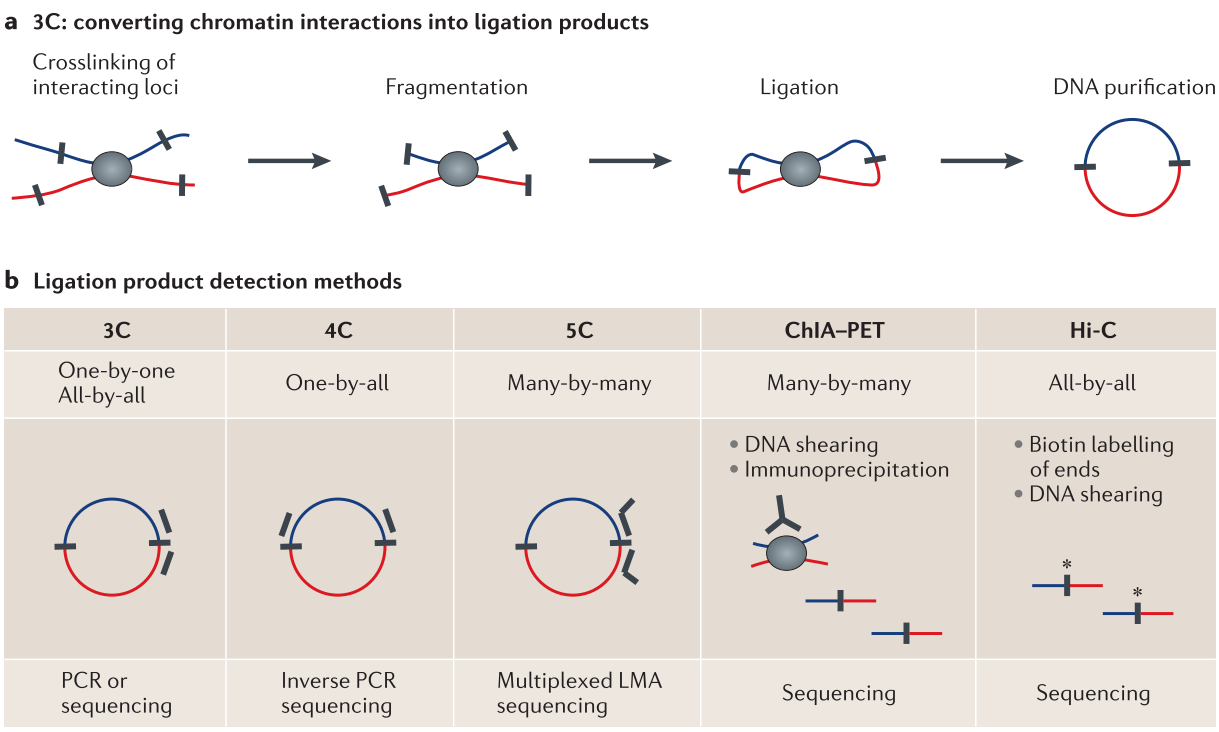
\includegraphics[width=0.8\linewidth]{figures/Dekker2013_3C} 

}

\caption{\textbf{Proximity ligation technologies to
measure chromatin interactions} \textbf{(A)} By treating cells with
formaldehyde chromatin is crosslinked. After fragmentation with
restriction enzymes, DNA from two loci in close physical proximity in
the nucleus is ligated to a hybrid DNA molecules that is than made from
DNA that originated from two regions distal in the linear genome
(indicated in red and blue). \textbf{(B)} Different variants of the 3C
experiments differ in their approaches to measure the ligation products
or subsets of it in order to quantify chromatin interactions. Figure
modified from \citep{Dekker2013}.}\label{fig:ProximityLigation}
\end{figure}












There exist several 3C-based methods which differ by the way the
ligation product, which represents and chromatin interaction, is
measured and quantified (Fig. \ref{fig:ProximityLigation}B). The classic
3C protocol allows to quantify hybrid DNA-product by quantitative PCR
using specific primers to amplify the product junction
\citep{Dekker2002}. In Circular chromosome conformation capture (4C)
experiments, a circular PCR is used to amplify all hybrid DNA products
ligated with a desired restriction fragment, e.g.~a specific viewpoint
of interest. These products are than sequences to generate an
interaction profile measuring all interacting regions with this
viewpoint \citep{Simonis2006, Noordermeer2011}. Another variant of 3C,
Carbon copy chromosome conformation capture (5C), combines 3C with
hybrid capture approaches to identify up to millions of interactions in
parallel between two large sets of loci, for example between a set of
promoters and a set of distal regulatory elements
\citep{Dostie2006, Sanyal2012}. Some methods combine chromatin
immunoprecipitation to enrich for chromatin interactions between loci
bound by specific proteins of interest or marked by post-translational
histone modifications. One of these methods is chromatin interaction
analysis by paired-end tag sequencing (ChIA-PET), which allows for
genome-wide analysis of long-range interactions between sites bound by a
protein of interest \citep{Fullwood2009}. Therefore, ChIA-PET data
represent a selected subset of all interactions, but is an efficient
alternative to measure interactions at very high resolution
\citep{Tang2015}. The most unbiased method to quantify all pair-wise
interactions genome-wide is Hi-C \citep{Lieberman-Aiden2009}. After the
initial restriction enzyme step of 3C, in Hi-C, the ends are filled with
a biotin-marked nucleotide and subsequently re-ligated. A streptavidin
pull-down step is used to enrich for the chimeric products, which are
than sequenced using paired-end sequencing technology. Each read from
the resulting read-pairs is than aligned independently to the reference
genome to identify the originating position of the sequenced restriction
fragment. Thereby each read pair represent a pairwise physical
interaction of the corresponding regions. Interaction frequencies are
usually analyzed by binning the genome into equal sized regions several
kb depending on sequencing depth. While the first Hi-C study produced
genome-wide interactions at 1Mb resolution \citep{Lieberman-Aiden2009},
more recent studies could analyse folding patterns at 40kb
\citep{Dixon2012}, and later up to 1kb resolution \citep{Rao2014}.

\section{Hierarchy of chromatin 3D
structure}\label{hierarchy-of-chromatin-3d-structure}

\begin{itemize}
\tightlist
\item
  Chromosomal Territories
\item
  A/B-Compartments
\item
  TADs
\item
  Chromatin Loops

  \begin{itemize}
  \tightlist
  \item
    Enhancer-Promoter loops
  \item
    Gene Loops
  \item
    Architectural loops
  \end{itemize}
\item
  Architectural Proteins
\item
  (Loop extrusion model)
\item
  Nucleosomes / 10nm / 30nm fibers
\end{itemize}

\begin{figure}

{\centering 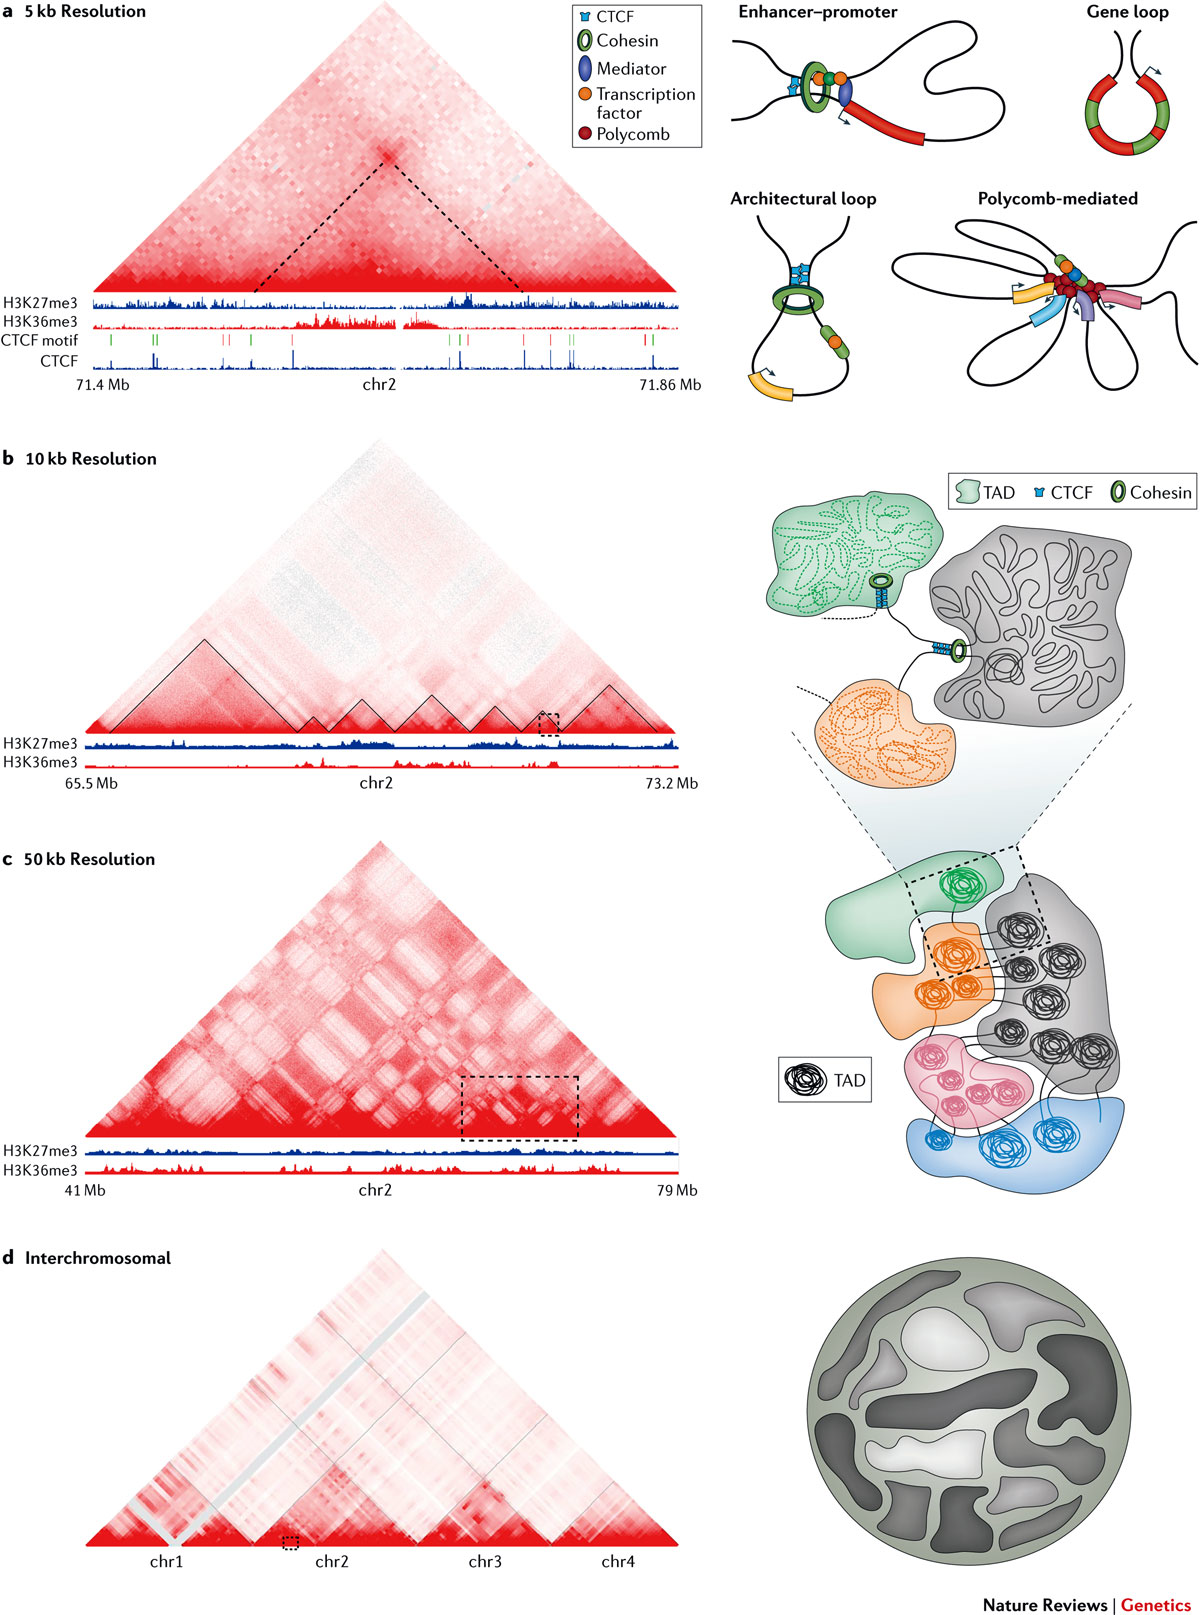
\includegraphics[width=0.8\linewidth]{figures/Bonev2016Fig2} 

}

\caption{\textbf{Hierarchical organization of chromatin
three-dimensional chromatin architecture} \textbf{(A)}\\
Figure source \citep{Bonev2016}
\url{https://www.nature.com/articles/nrg.2016.112/figures/2}.}\label{fig:GenomeHierarchy}
\end{figure}






\subsection{Chromosomal territories and inter-chromosomal
contacts}\label{chromosomal-territories-and-inter-chromosomal-contacts}

The eukaryotic genome is highly organized in the interpahse nucelus.
Chromosomes occupy distinct spatial regions, called chromosome
territories, and intermingle less than one would expect by chance
\citep{Cremer2001}. This was first observed using imaging based
approaches, and is reflected in Hi-C interaction maps, where
inter-chromosomal contacts occur order of magnitudes less frequent than
intra-chromosomal contacts \citep{Lieberman-Aiden2009}. However, despite
this spatial segregation of chromosome, intermingling of chromosome
occurs and is associated with chromosomal translocations
\citep[\citet{Roukos2013}, \citet{Roukos2014}]{Branco2006}. There are
also specific gene regulatory interactions between different chromosomes
\citep{DeLaat2007}, for example olfactory receptor genes cluster densely
in the nucleus of olfactory neurons to facilitate monoallelic expression
of a single receptor gene per cell \citep{Monahan2015}. While there are
specific inter-chromosomal contacts, the genome is non-randomly
organized in chromosomes which occupy distinct territories in the
spacial nucleus.

\subsection{A/B compartments}\label{ab-compartments}

The ability to measure genome-wide chromatin contacts using Hi-C,
revealed that individual regions on chromosomes segregate by
preferential interactions into two compartments mayor clusters, referred
to as A/B-compartments \citep{Lieberman-Aiden2009}. Interestingly,
regions A-compartments are associated with active histone-modifications
and active transcription, whereas B-compartment is associated with
heterochromatin, lamina association, and repressed genes.

\subsection{Topologically associating domains
(TADs)}\label{topologically-associating-domains-tads}

Compartments could be identified by clustering of long-range
interactions in Hi-C maps with bin resolution of 1 Mb. In 2012 higher
resolution Hi-C maps of up to 40 kb lead to the identification of
genomic regions with preferential interactions wiht them. These genomic
regions were termed topologically associating domains (TADs)
\citep{Dixon2012, Nora2012, Sexton2012}. They are opperationlly defined
as genomic regions with frequent interactions of loci within the domain
and decreased interactions across domain boundares \citep{Nora2016}.

TADs can be identified from Hi-C interaction maps computationally by
different algorithms \citep{Ay2015}. The directionality index is a score
for each bin in the Hi-C matrix that quantifies the number of upstream
versus downstream interactions of this bin. Using hidden Markov models
TAD boundaries where than identified in regions where DI is changing
drastically \citep{Dixon2012}. Other algorithms compute an insulation
score as the extent to which interactions to cross potential TAD
boundaries \citep{Crane2015}. Later the Arrowhead algorithm was
introduced to find ``contact domains'' as smaller nested structures
along the diagonal of high resolution Hi-C matrices \citep{Rao2014}.
Furthermore, when analyzing Hi-C interactions at differnt length scales,
hierarchies of TADs and sub-TADs could be identifed that overlap each
other \citep[\citet{Fraser2015}]{Filippova2014}.\\
The different algorithms and parameters used in each is only one source
of variation in reliably identifying TADs. Also the resolution of Hi-C
maps, which is mainly defined by sequencing depths but also the Hi-C
protocol itself \citep{Rao2015}, as well as different normalization
strategies for Hi-C contacts introduce variability \citep{Forcato2017}.
Therefore the number and size of TADs varies between different studies
and cannot be directly compared.

The first studies on TADs identifed around 3000 TADs in human and mouse
genomes with a median size of \textasciitilde{}800 kb \citep{Dixon2012}
and \textasciitilde{}100 kb in \emph{Drosophila} gneomes
\citep{Sexton2012}. Analysis of 1kb or 5kb resolution Hi-C matrixes
resulted in nested ``contact domains'' with median size of 185 kb (range
40 kb - 3 Mb) in human and mouse cells \citep{Rao2014}.

Importantly, TADs might be equivalent to ``chromatin domains'' of 10 kb
- 1 Mb in size detected by microscopy approaches
\citep{Cremer2010, Gibcus2013}. Annother connection of Hi-C derived
interaction maps with previous microscopy observations, is that TADs in
\emph{Drosophila} correspond to bands of polytene chromosomes
\citep{Eagen2015}.

The spatial positioning of TADs correlate with many genomic features
measured along the linear genome \citep{Merkenschlager2016}. TAD
boudnaries are enriched for binding of ``insulator protins'', such as
CTCF in mammals and CP190 in Drosophila \citep{Dixon2012, Sexton2012}.
Furthermore, TAD boundares are associated with active chromatin, such as
H3K4me3 and H3K27me3, DNase I hypersensivity, actie transcription, and
house-keeping genes \citep{Dixon2012}. Furthermore, TADs correspond to
regions of early and late replication timing
\citep{Pope2014, Dileep2015} and lamina associated domains (LADs)
\citep{Dixon2012}. Importantly, enhancer-promoter interactions seems to
be mostly constrained within TADs \citep{Shen2012}

There is acumulating evidence, that TADs are fundamental units of
chromosome organization \citep{Dixon2016}

\begin{itemize}
\tightlist
\item
  {[}X{]} Definition, number, and size
\item
  {[}X{]} Algorithms to identify TADs
\item
  Functional features
\item
  {[}X{]} CTCF binding at boundaries
\item
  {[}X{]} housekeeping genes at boundaries
\item
  enhancer-gene associations within TADs
\end{itemize}

\subsection{Chromatin loops}\label{chromatin-loops}

In summary, these findings suggest a hierarchical organization of
chromosome architecture. First, dynamic nucleosome contacts from
clutches and fibers. These engage in dynamic long-range chromatin loops,
some of which are stabilized by architectural proteins, such as CTCF and
cohesin, and lead to the formation of TADs. TADs in tern cluster by
their epigenomic type into A/B compartments and coalescence of
compartments in the same chromosome forms chromosome territories
\citep{Bonnev2016}.

\section{Dynamics of chromatin
structure}\label{dynamics-of-chromatin-structure}

\begin{itemize}
\tightlist
\item
  Cell-type invariant TADs\\
\item
  Conservation of TADs
\end{itemize}

\section{Changes of genome folding in evoltuion and disease
genomes}\label{changes-of-genome-folding-in-evoltuion-and-disease-genomes}

\begin{itemize}
\tightlist
\item
  Evolution of chromatin architecture
\item
  Disruption of chromatin architecture
\end{itemize}

\section{Aims of this thesis}\label{aims-of-this-thesis}

In this PhD thesis, I analyze TADs and chromatin interactions with
respect to gene expression regulation. More specifically, we find out
weather TADs represent only structural units of the genome or also
functional building blocks, in which genes regulation is coordinated.

\subsection*{Is the three-dimensonal folding of genomes associated with
co-regulation of functionally related
genes?}\label{is-the-three-dimensonal-folding-of-genomes-associated-with-co-regulation-of-functionally-related-genes}
\addcontentsline{toc}{subsection}{Is the three-dimensonal folding of
genomes associated with co-regulation of functionally related genes?}

\begin{itemize}
\tightlist
\item
  How are duplicated genes during evolution distributed in the
  three-dimensional genome architecture?
\item
  Can TADs provide regulatory environment for co-regulation of
  duplicated genes?
\item
  (Are TADs functional genomic units in which genes are co-regulated?)
\item
  (Are paralog genes co-regulated in the 3D chromatin architecture of
  genomes?)
\end{itemize}

\subsection*{Are TADs functional buidling blocks of genomes and
subjected to selective preasure during
evolution?}\label{are-tads-functional-buidling-blocks-of-genomes-and-subjected-to-selective-preasure-during-evolution}
\addcontentsline{toc}{subsection}{Are TADs functional buidling blocks of
genomes and subjected to selective preasure during evolution?}

\begin{itemize}
\tightlist
\item
  Are TADs conserved during evolution or disrupted by rearrangements?
\item
  Are changes of TADs during evolution associated with changes in gene
  expression profiles?
\item
  (Are TADs stable units that are often transmitted as a whole than
  disrupted by rearrangements?)
\end{itemize}

\subsection*{Is the disruption of TADs by rearrangements also associated
to genetic
diseases?}\label{is-the-disruption-of-tads-by-rearrangements-also-associated-to-genetic-diseases}
\addcontentsline{toc}{subsection}{Is the disruption of TADs by
rearrangements also associated to genetic diseases?}

\begin{itemize}
\tightlist
\item
  Can TADs be used to interpret position effects of rearrangements in
  genetic diseases?
\item
  Can chromatin interaction data and TADs be integrated with phenotype
  data to predict pathomechanism of balanced chromosomal rearrangements?
\end{itemize}

\subsection*{Can chromatin looping interactions be predicted by ChIP-seq
and sequence
features?}\label{can-chromatin-looping-interactions-be-predicted-by-chip-seq-and-sequence-features}
\addcontentsline{toc}{subsection}{Can chromatin looping interactions be
predicted by ChIP-seq and sequence features?}

\begin{itemize}
\tightlist
\item
  Are there signals form TF ChIP-seq data at chromatin looping anchors
  that predict long-range contacts?
\item
  Does the gnomic sequence encode features that are predictive for
  chromatin looping interactions?
\item
  Can we provide a computational method to predict chromatin looping
  interactions in specific cell-types and conditions of interest?
\end{itemize}

\section{Structure of this thesis}\label{structure-of-this-thesis}

These questions are addressed and discussed in the following for
chapters. First, we focus on duplicated genes in the human genome.
Because of their related sequence and function, shared evolutionary
history, and close co-localization in the genome they represent an
interesting model to study how genome folding is related to regulation
of gene expression during evolution (Chapter
\protect\hyperlink{ch:paralog_regulaion}{Paralog genes}). Furthermore,
we make use of deeply sequenced genomes of other vertebrates to
systematically investigate whether TADs represent conserved building
blocks of genomes and whether rearrangements are associated with altered
gene expression programs (Chapter
\protect\hyperlink{ch:TAD_evolution}{TAD evolution}). Next, we will
address disruption of chromatin organization by analyzing disease
associated rearrangement breakpoints from whole-genome sequenced
patients of various genetic diseases to explain miss-regulation by
disruption of TADs and chromatin contacts in diseases (Chapter
\protect\hyperlink{ch:position_effect}{Position effect}). Finally, we
will make use of recent insights in chromatin loop formation to provide
a computational tool to predict chromatin loops from largely available
genomic data, with the aim to facilitate association of TF binding sites
in enhancers to regulated genes in many cell-types and condition, for
which Hi-C like data is not available (Chapter
\protect\hyperlink{ch:loop_prediction}{Loop prediction}).

\hypertarget{ch:paralog_regulaion}{\chapter{Paralog genes in the 3D
genome architecture}\label{ch:paralog_regulaion}}

This chapter is published in Nucleac Acid Research
\citep{Ibn-Salem2017}. The surce code for the complete analysis is
available at GitHub:
\url{https://github.com/ibn-salem/paralog_regulation}

\section{Introduction}\label{introduction}

Paralog genes arise from gene duplication events during evolution. The
resulting sequence similarity between paralog pairs might lead to
similar structure and function of encoded proteins \citep{Koonin2005}.
Since paralogs often form part of the same protein complexes and
pathways, it is advantageous for the cell to coordinate their expression
\citep{Makova2003}.

In eukaryotes, genes are regulated in part by binding of transcription
factors to promoter sequences and to distal regulatory regions such as
enhancers. By chromatin looping, enhancer bound proteins can physically
interact with the transcription machinery at the promoter of
genes~\citep{Ptashne1986, Deng2012, Carter2002, Tolhuis2002, Spitz2012}.
These chromatin looping events can be measured by chromatin conformation
capture (3C) experiments~\citep{Dekker2002}, which use
proximity-ligation, and more recently high-throughput sequencing (Hi-C)
to measure DNA-DNA contact frequencies
genome-wide~\citep{Lieberman-Aiden2009}.

These interaction maps revealed tissue-invariant chromatin regions,
named topologically associating domains (TADs), which have more
interactions within themselves than with other
regions~\citep{Dixon2012, Nora2012, Sexton2012}. TADs seem to be stable
across cell types and conserved between
mammals~\citep{Dixon2012, Rao2014, VietriRudan2015}. Regions within TADs
show concerted histone chromatin
signatures~\citep{Dixon2012, Sexton2012}, gene
expression~\citep{LeDily2014, Nora2012}, and DNA replication
timing~\citep{Pope2014}. Furthermore, disruption of TAD boundaries is
associated to genetic diseases~\citep{Ibn-Salem2014, Lupianez2015}.

We wondered if the Hi-C data could reveal evolutionary pressure driving
paralogous expansion to favour the clustering of paralogs in the
three-dimensional chromatin architecture and their regulation by common
enhancer elements to enable the cell to fine-tune and coordinate their
expression. To do this, we collected Hi-C data from a number of studies
profiling contacts in several cell types from
human~\citep{Dixon2012, Rao2014}, mouse and dog~\citep{VietriRudan2015},
and we compared the properties of these data with respect to paralog
genes. Our results pinpoint that pairs of paralog genes tend to be
co-regulated and co-occur within TADs more often than equivalent control
gene pairs. When placed in different TADs, paralogs still tend to
co-occur in the same chromosome and have more contacts than control gene
pairs. In contrast, close paralogs in the same TAD have significantly
less contacts with each other than comparable gene pairs, which could
indicate that these pairs of paralogs encode proteins that functionally
replace each other.

These observations have relevance for the study of the evolution of
chromatin structure and suggest that tandem duplications generating
paralogs are under selection according to how they contribute or not to
the fine structure of the genome as reflected by TADs. Thus TADs provide
a favorable environment for the co-regulation of duplicated genes, which
is likely followed by the evolutionary generation of additional
regulatory mechanisms allowing the separation of paralogs into different
TADs in the same chromosome but connected, and eventually their
migration into different chromosomes.

\section{MATERIALS AND METHODS}\label{sec:paralog-methods}

\subsection{Selection of pairs of paralog
genes}\label{selection-of-pairs-of-paralog-genes}

All human genes and human paralog gene pairs were retrieved from Ensembl
GRCh37 (Ensembl 75) database by using the \texttt{biomaRt}
package~\citep{Durinck2009b, Durinck2005} from within the statistical
programming environment R. For each gene we downloaded the Ensembl gene
ID, HGNC symbol, transcription sense, transcription start site (TSS)
coordinates, and gene length. We only considered protein coding genes
with ``KNOWN'' status that are annotated in the 22 autosomes or the 2
sexual chromosomes. For each gene we used the earliest TSS coordinate.
Within this set of genes, all pairs of human paralog genes were
downloaded from Ensembl~\citep{Vilella2009}. This resulted in a total of
19,430 human genes; more than half of those had at least one human
paralog gene (Fig.~\ref{fig:paraVSnonPara}A).

However, many human genes have more than one paralog
(Fig.~\ref{fig:paraVSnonPara}B). To avoid overrepresentation of genes,
we filtered the pairs such that each gene occurred only once. Thereby we
selected the pairs by minimizing the rate of synonymous mutations (dS)
between them using a maximum-weighted matching graph algorithm implement
in the python package \texttt{NetworkX}~\citep{Galil1986}. The number of
synonymous mutations between paralogs has been used to approximate the
duplication age~\citep{Lan2016}. Therefore our implementation favours
the selection of young paralog pairs for larger paralog families and
guaranties that each gene occurs only once. This filtering strategy
resulted in \(6256\) unique paralog pairs for downstream
analysis~(Table~\ref{tab:filter}). We observed that modications of this
strategy to select unique paralog genes did not affect essentially the
results of our study (e.g.~by selecting pairs while maximising dS;
Fig.~\ref{fig:selectOldPairs}).

Analogously to the human data we downloaded all pairs of protein coding
paralog genes from the \emph{Mus musculus} (GRCm38.p2) and \emph{Canis
lupus familiaris} (CanFam3.1) genomes from Ensembl. The numbers of
filtered gene pairs are shown in Table \ref{tab:filter}~. Furthermore,
we related human paralog genes to orthologs in mouse and dog only if
there was a unique one-to-one orthology relationship reported in the
Ensembl database.

\begin{longtable}[]{@{}lrrc@{}}
\caption{\label{tab:filter} Filtering of human paralog gene
pairs}\tabularnewline
\toprule
Paralog pairs & Human & Mouse & Dog\tabularnewline
\midrule
\endfirsthead
\toprule
Paralog pairs & Human & Mouse & Dog\tabularnewline
\midrule
\endhead
All paralog pairs & 46546 & 110490 & 28293\tabularnewline
One pair per gene & 6256 & 7323 & 4959\tabularnewline
On the same chromosome & 1560 & 2397 & 658\tabularnewline
Close pairs (TSS distance \(\leq\) 1 Mb) & 1114 & 1774 &
455\tabularnewline
Distal pairs (TSS distance \(>\) 1 Mb) & 446 & 623 & 203\tabularnewline
\bottomrule
\end{longtable}

\subsection{Enhancers to gene
association}\label{enhancers-to-gene-association}

Human enhancer annotations, including their genome locations and the
corresponding genes they regulate, were obtained from the supplementary
data of a recent CAGE analysis~\citep{Andersson2014}. In this study, the
activity of enhancers and genes was correlated within 500kb over
hundreds of human cell types to provide a regulatory interaction map
between 27,451 enhancers and 11,604 genes consisting of 66,942
interactions.

\subsection{Topological associating
domains}\label{topological-associating-domains}

We obtained topological associating domain (TAD) calls from two recently
published Hi-C studies in human cells~\citep{Dixon2012, Rao2014}. TAD
locations mapped to the hg18 genome assembly were converted to hg19
using the UCSC liftOver tool~\citep{Hinrichs2006}. A/B-compartment and
sub-compartment annotations were obtained from high-resolution Hi-C
experiments in human GM12878 cells~\citep{Rao2014}.

\subsection{Hi-C interaction maps}\label{hi-c-interaction-maps}

Individual chromatin-chromatin contact frequencies from IMR90 cells at 5
kb resolution were retrieved from~\citep{Rao2014}(NCBI GEO accession:
GSE63525). We used only reads with mapping quality \(\geq\) 30 and
normalized the raw contact matrices applying the provided normalization
vectors for KR normalization by the matrix balancing
approach~\citep{Knight2013}. We only considered pairwise gene
interactions if the TSSs of the two genes were located in different bins
of the Hi-C matrix with normalized contacts \(\geq\) 0. Capture Hi-C
data between promoter regions in human GM12878 cells were downloaded
from ArrayExpress (accession: E-MTAB-2323)~\citep{Mifsud2015}.

\subsection{Randomization}\label{randomization}

We analysed the distribution of paralog pairs over chromosomes depending
on the linear distance between them. For doing so, we sampled gene pairs
from all human genes with equal and independent probability and refer to
them as random gene pairs.

For strand analysis, co-localisation in TADs, and Hi-C contact
quantification between paralog pairs, we constructed a carefully sampled
control set of gene pairs as null-model. Thereby we accounted for the
linear distance bias observed for paralog pairs. First, we calculated
all possible non-overlapping pairs of human genes on the same
chromosome. From the resulting set of gene pairs we randomly sampled
pairs according to the linear distance distribution of paralog gene
pairs. Therefore, we assigned to each gene pair a sampling weight that
is proportional to the probability to sample the pair. The sampling
weight \(w(g_{i}, g_{j})\) for a given pair of genes \(g_{i}\) and
\(g_{j}\) with absolute distance \(d_{i,j}\) is defined as

\[
w(g_{i}, g_{j}) = \frac{ f_{\mathrm{paralogs}}(d_{i,j}) }{f_{\mathrm{all}}(d_{i,j})}
\]

where \(f_{\mathrm{paralogs}}\) is the observed frequencies of distances
in the paralog genes and \(f_{\mathrm{all}}(d_{i,j})\) the frequency of
pairwise distances in the population of gene pairs from which we sample.
We computed the observed frequencies by dividing the distances into 90
equal-sized bins after \(log_{10}\) distance transformation and counted
occurrences of gene pairs for each bin. The resulting sampling weights
for all gene pairs are normalized to sum up 1 and were then used as
probabilities for sampling:

\[
p_{\mathrm{dist}}(g_{i}, g_{j}) = \frac{ w(g_{i}, g_{j}) }{ \sum_{i,j} w(g_{i}, g_{j}) }
\label{eq:DistProb}
\]

Next, for comparison of shared enhancers we slightly modified the
sampling of gene pairs to account for the observation that paralogs tend
to be associated to more enhancers than non-paralogs
(Fig.~\ref{fig:paraVSnonPara}D). Assuming that the number of enhancers
associated to genes is independent from the distance, we computed
sampling probabilities by \[
p_{\mathrm{dist+eh}}(g_{i}, g_{j}) = p_{\mathrm{dist}}(g_{i}, g_{j}) \cdot p_{\mathrm{eh}}(n_{i}) \cdot p_{\mathrm{eh}}(n_{j})
\] whereby \(n_{i}\) and \(n_{j}\) are the number of enhancers
associated to \(g_{i}\) and \(g_{j}\), respectively and
\(p_{\mathrm{eh}}(n)\) is the probability to sample a gene associated to
n enhancers:

\[
p_{\mathrm{eh}}(n) = \frac{ w_{\mathrm{eh}}(n) }{ \sum_{i=0}^{N} w_{\mathrm{eh}}(i) }
\label{eq:EhProb}
\]

and \[
w_{\mathrm{eh}}(n) = \frac{ f_{\mathrm{paralogs}}(n) }{f_{\mathrm{all}}(n)}
\]

where \(f_{\mathrm{paralogs}}(n)\) and \(f_{\mathrm{all}}(n)\) gives the
frequency of genes associated to \(n\) enhancers observed in the paralog
pairs and all gene pairs, respectively.

Analogously, we sampled sets of pairs accounting additionally for the
observed bias in paralog pairs to be in the same strand. \[
p_{\mathrm{dist+eh+strand}}(g_{i}, g_{j}) = p_{\mathrm{dist}}(g_{i}, g_{j}) \cdot p_{\mathrm{eh}}(n_{i}) \cdot p_{\mathrm{eh}}(n_{j}) \cdot p_{\mathrm{strand}}(s_{i,j})
\] whereby \(s_{i,j}\) is \(1\) if both genes, \(g_{i}\) and \(g_{j}\),
are transcribed from the same strand and \(0\) otherwise. The
probability \(p_{\mathrm{strand}}(s_{i,j})\) is computed in the same way
as the probability by number of enhancers \(p_{\mathrm{eh}}(n)\) in
equation \eqref{eq:EhProb}.

Lastly, we sampled a set of gene pairs by taking additionally the gene
length into account and computed sampling probabilities by \[
p_{\mathrm{dist+eh+len}}(g_{i}, g_{j}) = p_{\mathrm{dist}}(g_{i}, g_{j}) \cdot p_{\mathrm{eh}}(n_{i}) \cdot p_{\mathrm{eh}}(n_{j}) \cdot p_{\mathrm{len}}(l_{i}) \cdot p_{\mathrm{len}}(l_{j})
\]

whereby \(p_{\mathrm{len}}(l)\) for gene length \(l\) is computed in the
same way as for distances between gene pairs
(equation~\eqref{eq:DistProb}) and by dividing gene lengths into 20 equal
sized binds after \(log_{10}\) transformation of gene lengths in bp.

For each paralog pair on the same chromosome within 1 Mb distance, we
sampled \(10\) random gene pairs with this procedures each resulting in
\(n=156,000\) sampled gene pairs that served as background in our
statistical analysis. These sampling approaches resulted in similar
distribution of linear distances (Fig.~\ref{fig:samplingDist}),
associated enhancers of each gene (Fig.~\ref{fig:samplingDistEh}), same
strand (Fig.~\ref{fig:samplingDistEhStrand}), and gene lengths
(Fig.~\ref{fig:samplingDistEhLen}).

\subsection{Statistical tests}\label{statistical-tests}

We compared observed fractions of gene pairs, on the same chromosome,
with the same transcription sense, within the same TAD or compartment,
and with at least one shared enhancer between pairs of paralogs and
random or sampled pairs using the Fisher's exact test. Hi-C contact
frequencies and genomic distances between TSS of gene pairs were
compared using a Wilcoxon rank-sum test. All analyses were carried out
in the statistic software R version 3.2.2.

\section{RESULTS}\label{results}

\subsection{Distribution of paralog genes in the human
genome}\label{distribution-of-paralog-genes-in-the-human-genome}

Paralogs are homologous genes that arise from gene duplication events.
Their common ancestry and replicated sequence often leads to similar
structure and function in related pathways and protein complexes. We
therefore hypothesised that the transcription of paralogs should have a
tendency for co-regulation, which could correspond to their position in
the genome and within TADs. To test this hypothesis, we first focused on
the positions of paralogs in the linear genome.

From all \(19,430\) protein coding genes in the human genome,
\(13,690~(70.5\%)\) have at least one paralog
(Fig.~\ref{fig:paraVSnonPara}A). However, many human genes have several
paralogs (Fig.~\ref{fig:paraVSnonPara}B). From all \(46,546\) paralog
gene pairs we filtered for only one pair per gene \((n=6,256)\) and
further for non-overlapping pairs on the same chromosome \((n=1,560)\)
(see ). We will refer to close paralogs if their transcription start
sites (TSSs) are within 1 Mb of each other \((n=1,114)\) and to distal
pairs for paralogs with TSSs separated by more than 1 Mb \((n=446)\)
(Table~\ref{tab:filter}).

We first compared basic properties between genes that have at least one
paralog copy and genes without human paralogs. Paralogs have
significantly larger gene length than non-paralog genes
(\(p = 1.7 \times 10^{-53}\), Wilcoxon rank-sum test,
Fig.~\ref{fig:paraVSnonPara}C), which fits the observation
from~\citep{He2005} in yeast. Furthermore, paralogs tend to be
associated to more enhancers compared to non-paralog genes (on average
\(3.8\) vs. \(2.5\) enhancers per gene, \(p=2.89\times10^{-70}\),
Fig.~\ref{fig:paraVSnonPara}D) and the distance to the nearest
associated enhancer is significantly shorter
(\(p=2.71\times10^{-22}\),Fig.~\ref{fig:paraVSnonPara}E).

Since most genome duplication events in humans emerge through tandem
duplications~\citep{Newman2015}, we expected some co-localization among
pairs of paralog genes. Indeed \(24.9\%\) of paralog pairs are located
on the same chromosome. We compared this to random expectation by
sampling random gene pairs from all protein coding human genes and found
only \(5.3\%\) of randomly sampled gene pairs on the same chromosome
(\(p<10^{-16}\), Fig.~\ref{fig:paraData}A).

\begin{figure}

{\centering 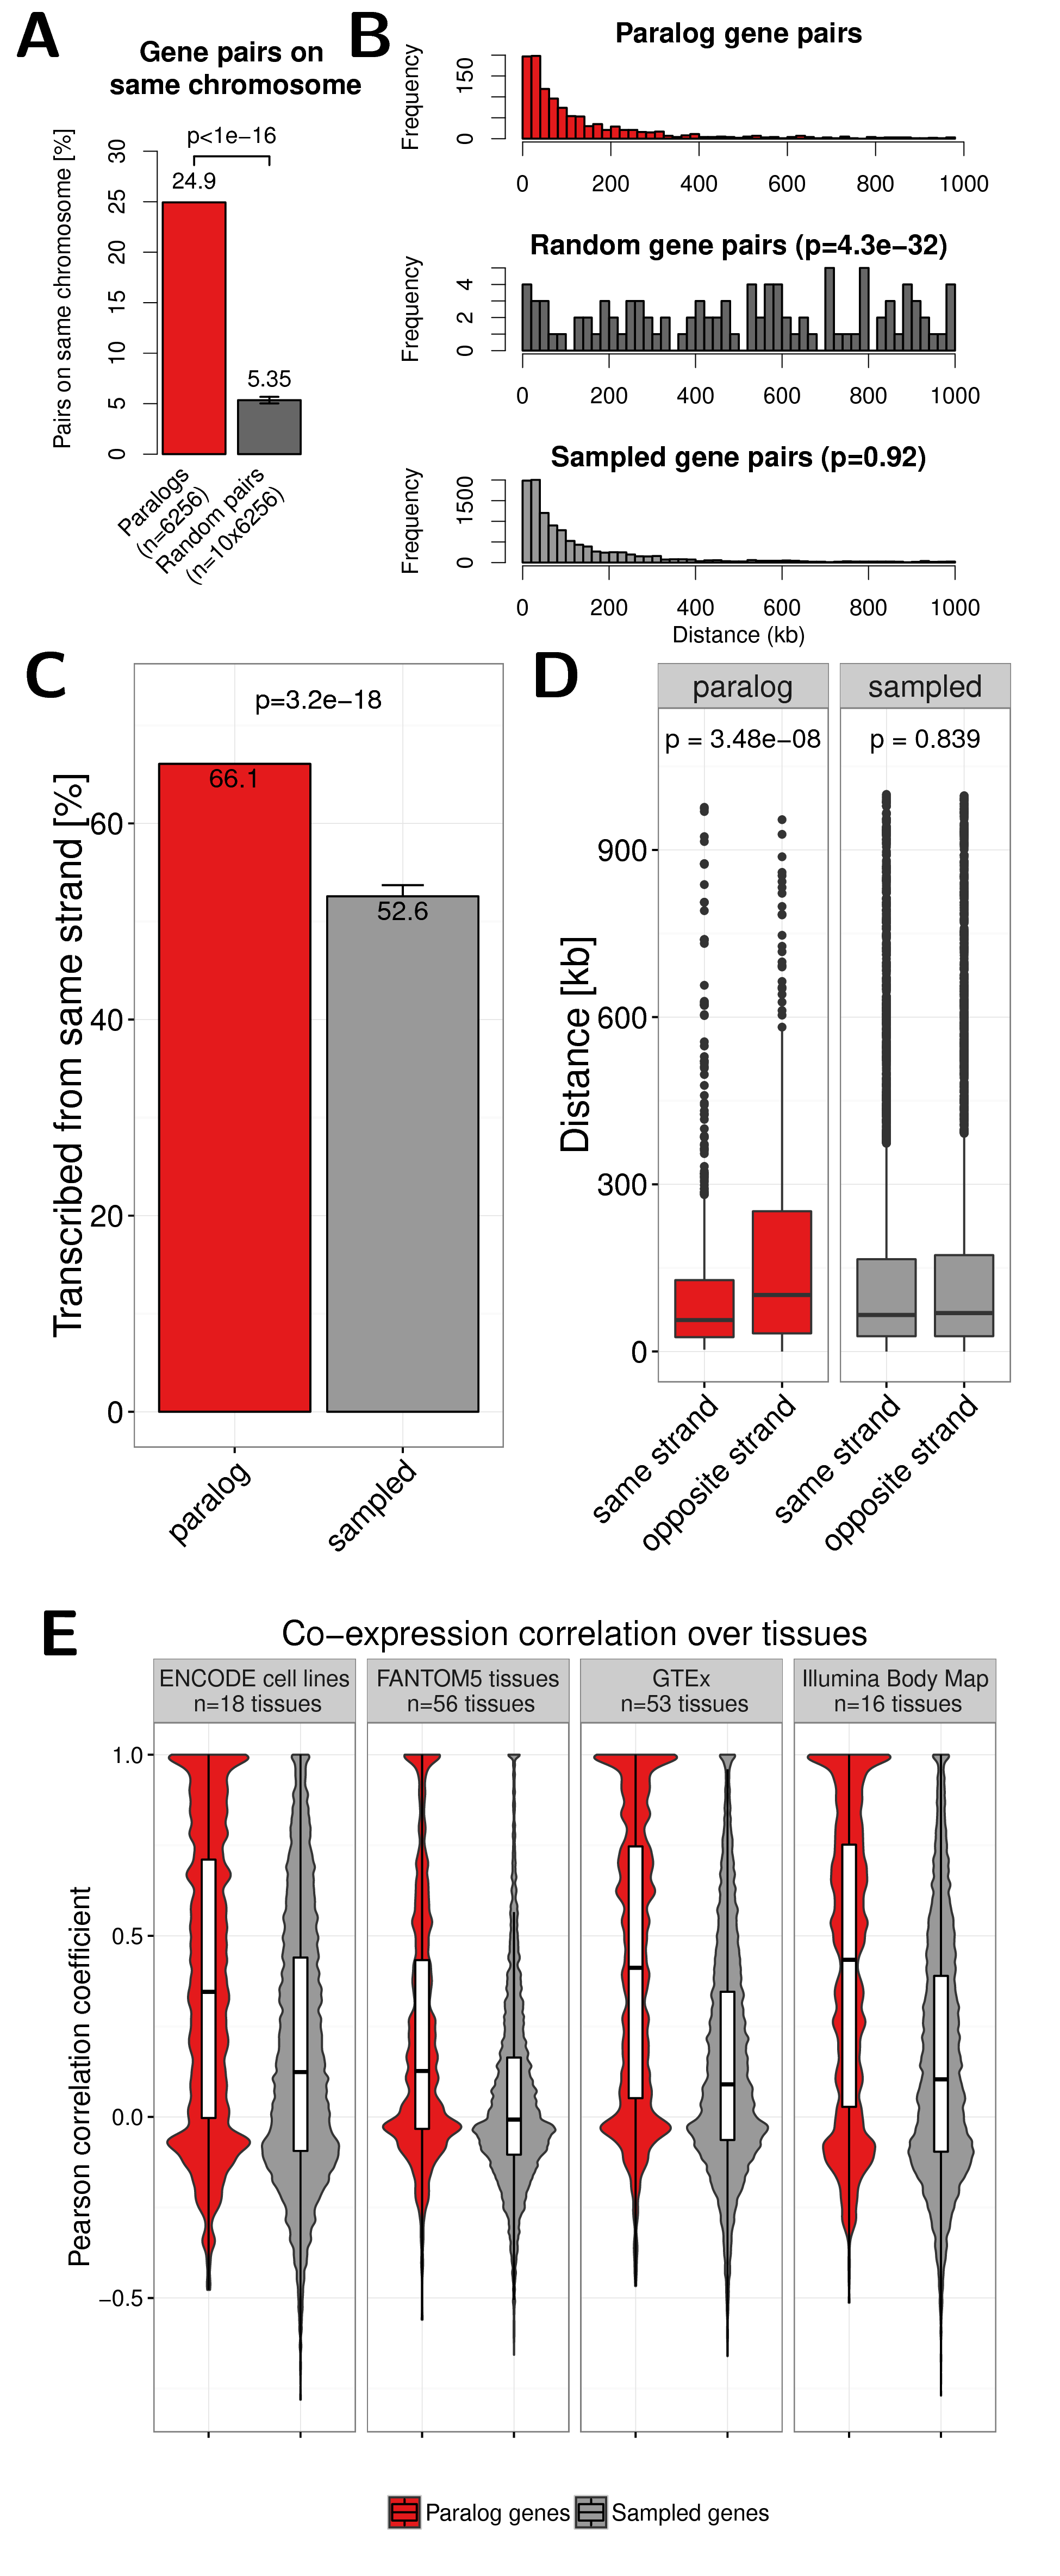
\includegraphics[width=0.5\linewidth]{figures/paralog/fig1_09} 

}

\caption{\textbf{(A)} Percent of paralog (red) and random (dark
grey) gene pairs that are located on the same chromosome. The error bar
indicates the standard deviation observed in 10 times replicated random
sampling of gene pairs. \textbf{(B)} Genomic distance distribution of
paralogs gene pairs (top), random gene pairs (center) and gene pairs
sampled according to distance distribution of paralogs (bottom).
Distances are measured in kilo base pairs (kb) between TSS of genes in
pairs. P-values are calculated using Wilcoxon rank-sum test.
\textbf{(C)} Percent of paralog (red) and sampled (grey) gene pairs that
are transcribed from the same strand. Only pairs on the the same
chromosome within 1 Mb are considered here. Error bars indicate the
standard deviation observed in 10 times replicated sampling of gene
pairs. \textbf{(D)} Boxplot of the genomic distance between paralogs and
sampled gene pairs with the same or opposite strands. \textbf{(E)}
Distribution of Pearson correlation coefficients of gene expression
values in four independent data sets between paralog gene pairs (red)
and sampled control gene pairs (grey). White boxes show 25th, 50th and
75th percent quantile of the data and the filled areas indicate the
density distribution..}\label{fig:paraData}
\end{figure}





















We further analysed whether paralog pairs tend to be located in close
genomic distance on the same chromosomes. We compared the distance
between paralog gene pairs to the distance of completely random genes on
the same chromosome. As expected there is a strong bias of genomic
co-localization among paralog gene pairs that is not observed for random
gene pairs (\(p=4.3\times10^{-32}\), Fig~\ref{fig:paraData}B).

We also observed that close paralog genes show more often than expected
the same transcription orientation. From all paralog pairs within 1 Mb
on the same chromosome \(66.1\%\) have the same sense. This is
significantly more than for randomly sampled genes with the same
distance (52.6\%, \(p=3.2\times10^{-18}\), Fig.~\ref{fig:paraData}C).

Furthermore, we observed that paralogs in the same strand are closer to
each other on the chromosome than pairs in opposite strands
(\(p=3.48\times10^{-8}\), Fig.~\ref{fig:paraData}D).

Together, this shows that paralogs tend to be located within short
linear distance on the same chromosome and same transcription sense,
which might enable coordinated regulation by shared regulatory
mechanisms.

\subsection{Co-expression of paralog gene pairs across
tissues}\label{co-expression-of-paralog-gene-pairs-across-tissues}

To assess whether paralog genes tend to be indeed co-regulated we
compared gene expression of paralog gene pairs over several human
tissues and cell lines.

We compared the Pearson correlation coefficient (PCC) of gene expression
values over \(n = 18\) cell-lines analysed by the ENCODE consortium by
RNA-seq~\citep{Djebali2012}. The distribution of PCC among paralog genes
is bimodal with one peak around \(-0.1\) and another at nearly \(1.0\),
which indicates that there exists a group of paralog pairs without
expression correlation and that the expression of other paralogs is
highly positively correlated. Notably, we did not find the latter signal
for positive correlation in our control set of carefully sampled gene
pairs (Fig.~\ref{fig:paraData}E).

We repeated the analysis with three other independent gene expression
data sets form FANTOM5 (\(n=56\) tissues)~\citep{Forrest2014}, GTEx
(\(n=53\) tissues)~\citep{GTExConsortium2015} and the Illumina Body Map
(\(n=16\) tissues), which we retrieved from the EBI Expression
Atlas~\citep{Petryszak2015}. In all data sets we found more positively
correlated paralog pairs compared to the sampled gene pairs
(Fig.~\ref{fig:paraData}E). This shows that many paralogs are expressed
with high coordination in a tissue specific manner.

\subsection{Paralog genes share
enhancers}\label{paralog-genes-share-enhancers}

We hypothesised that common gene regulation of close paralog genes is
likely to be facilitated by shared enhancer elements. Indeed we found
that paralog gene pairs within 1 Mb on the same chromosome are
associated to the same enhancer elements more often than expected by
chance (Fig.~\ref{fig:sharedEnhancer}). We estimated the expected
background distribution of shared enhancers by carefully sampling gene
pairs with the same distributions as paralogs in distances and
associated enhancers to single genes (Fig.~\ref{fig:samplingDistEh},
section \ref{sec:paralog-methods}).

\begin{figure}

{\centering 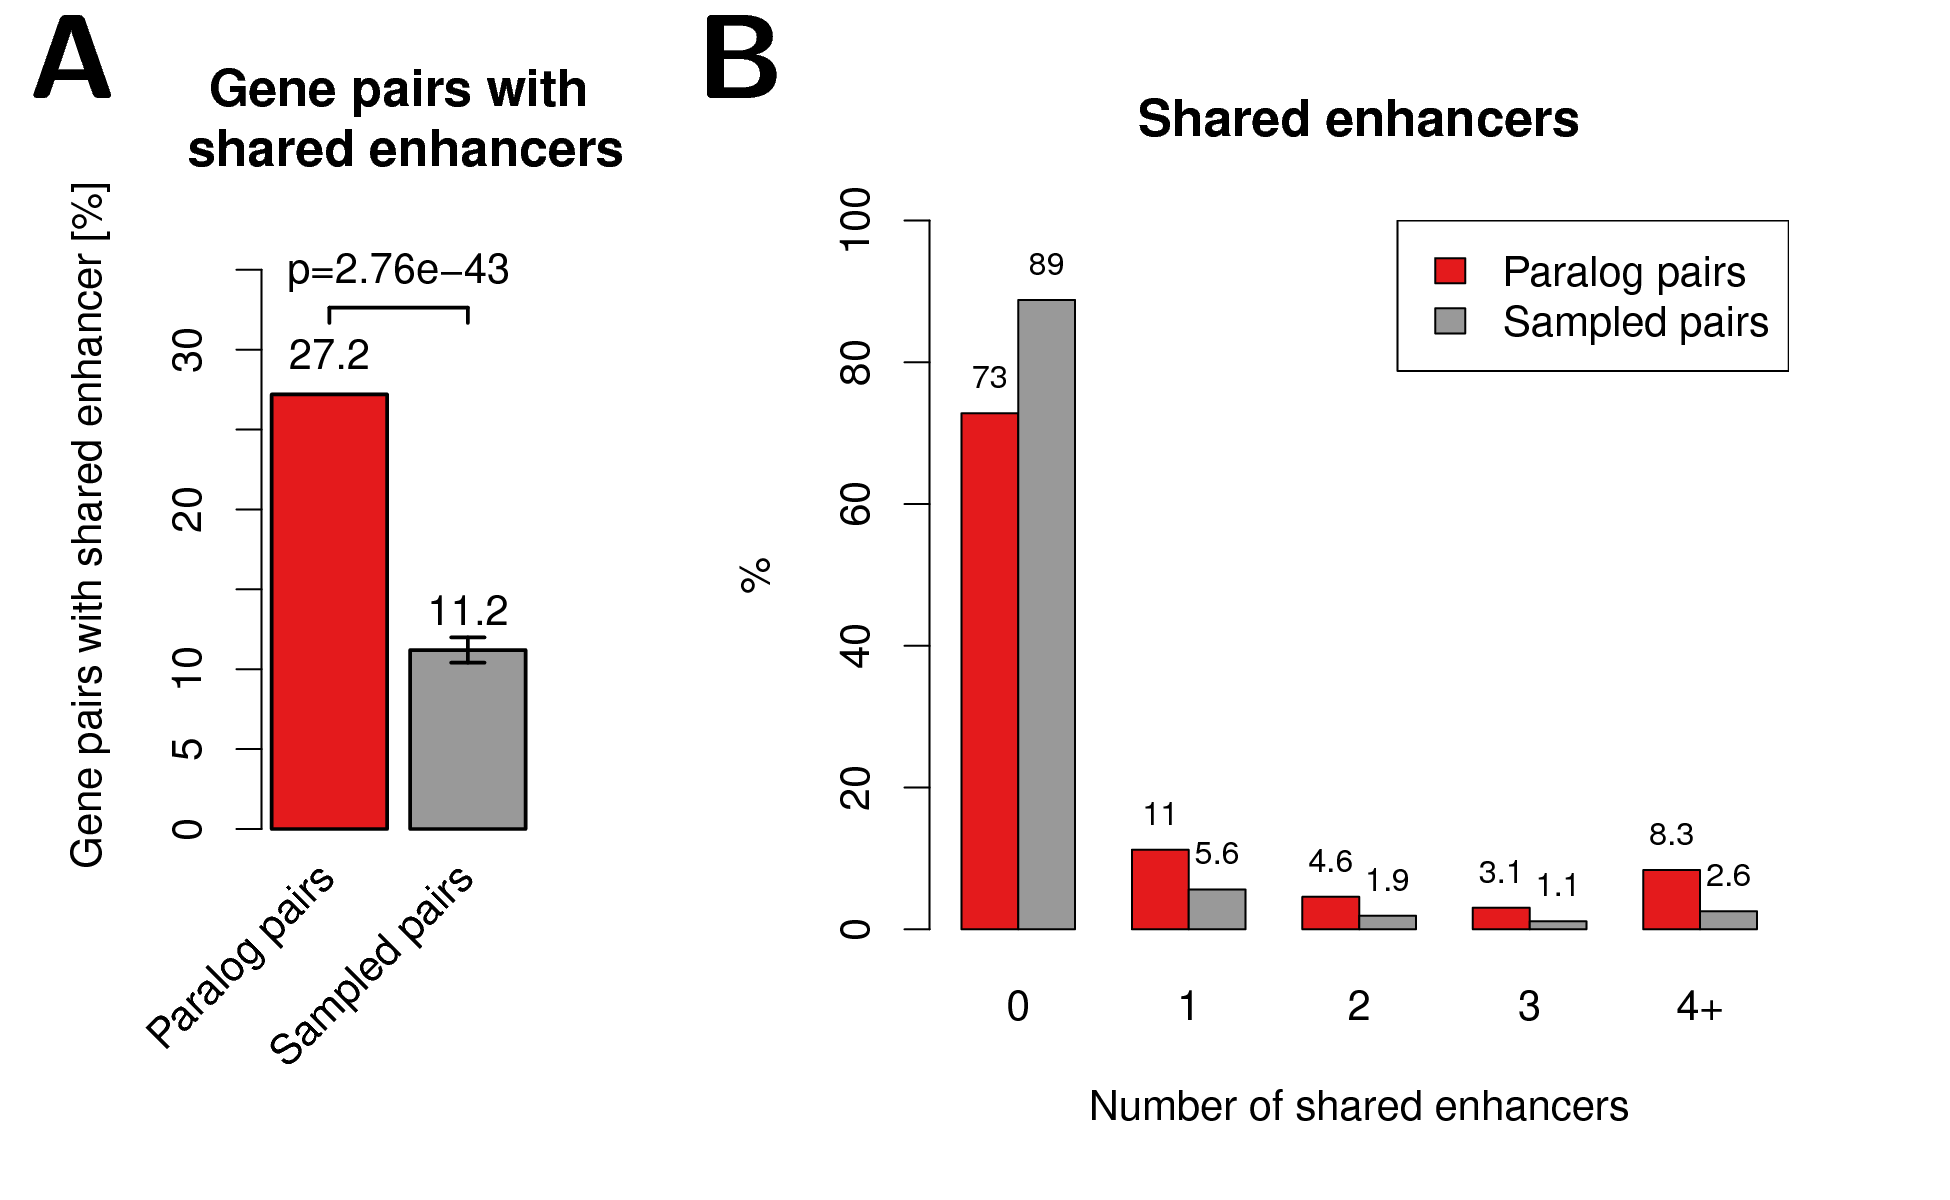
\includegraphics[width=0.5\linewidth]{figures/paralog/fig2_09} 

}

\caption{Shared enhancers among paralog gene pairs.
\textbf{(A)} Percent of close paralog (red) and sampled control (grey)
gene pairs with at least one shared enhancer. \textbf{(B)} Percent of
gene pairs versus number of shared enhancers for paralog and sampled
control gene pairs.}\label{fig:sharedEnhancer}
\end{figure}







While \(27.2\)\% of the paralog gene pairs have at least one enhancer in
common, we observed this for only \(11.7\)\% of the sampled gene pairs
(\(p=4.2\times10^{-40}\), Fig.~\ref{fig:sharedEnhancer}A). This could be
replicated when comparing against sampled gene pairs where in addition
to distance and number of enhancers linked to single genes, also the
transcription sense and gene length were taken into account during
sampling of control gene pairs (\(p=3.4\times10^{-41}\) and
\(p=5\times10^{-30}\), respectively; Fig.~\ref{fig:ehBySampType}). Next,
we compared the percent of gene pairs with shared enhancers as a
function of the number of shared enhancers between paralogs and sampled
gene pairs. We observed that paralog pairs are enriched for higher
number of shared enhancers compared to the sampled gene pairs
(Fig.~\ref{fig:sharedEnhancer}B). Together, these results indicate that
paralog genes are more often co-regulated by common enhancer elements
than other genes.

\subsection{Co-localization of paralogs in
TADs}\label{co-localization-of-paralogs-in-tads}

To facilitate their function in gene regulation, distal enhancer
elements need to interact physically via chromatin looping with promoter
elements at the TSS of their target genes. These looping interactions
occur frequently within so called topological associating domains
(TADs). These are regions of hundreds of kb that show high rates of
self-interactions and few interactions across domain boundaries in
genome-wide Hi-C experiments~\citep{Dixon2012, Rao2014}. Genes within
the same TAD are therefore likely to have common gene regulatory
programs \citep{LeDily2014, Nora2012}.

We used TADs from Hi-C experiments in eight different human cell-types
(HeLa, HUVEC, K562, KBM7, NHEK, IMR90, GM12878, and hESC) from two
recent studies ~\citep{Dixon2012, Rao2014}. Notably, the called TADs
differ in size between the two publications due to different resolution
of Hi-C experiments and different algorithms used to call them from Hi-C
contact matrices (Fig.~\ref{fig:TADsize}). TADs from~\citep{Rao2014}
have a median size of around 240 kb and are nested, so that several
small domains can occur within one ore more larger domains. In contrast
TADs from~\citep{Dixon2012} are of 1 Mb on average and are defined as
non-overlapping genomic intervals.

We hypothesised that paralog gene pairs might be located more often in
the same TAD than expected by chance. Indeed, we found that, depending
on cell-type and study, between \(35\%\) and \(73\%\) of close paralog
pairs are located in the same TAD (Fig.~\ref{fig:TAD}A). In seven out of
nine data sets this difference was significant (\(p<0.05\)) with respect
to the sampled control gene pairs with the same linear distance. We also
calculated a set of \(n=2,624\) stable TADs that are found in more than
50\% of cell types analysed in \citep{Rao2014}. Notably, we found for
paralog pairs a \(1.25\) fold enrichment to be located in the same
stable TADs compared to sampled gene pairs (\(p=0.00013\), stable\_TADs
in Fig.~\ref{fig:TAD}A).

\begin{figure}

{\centering 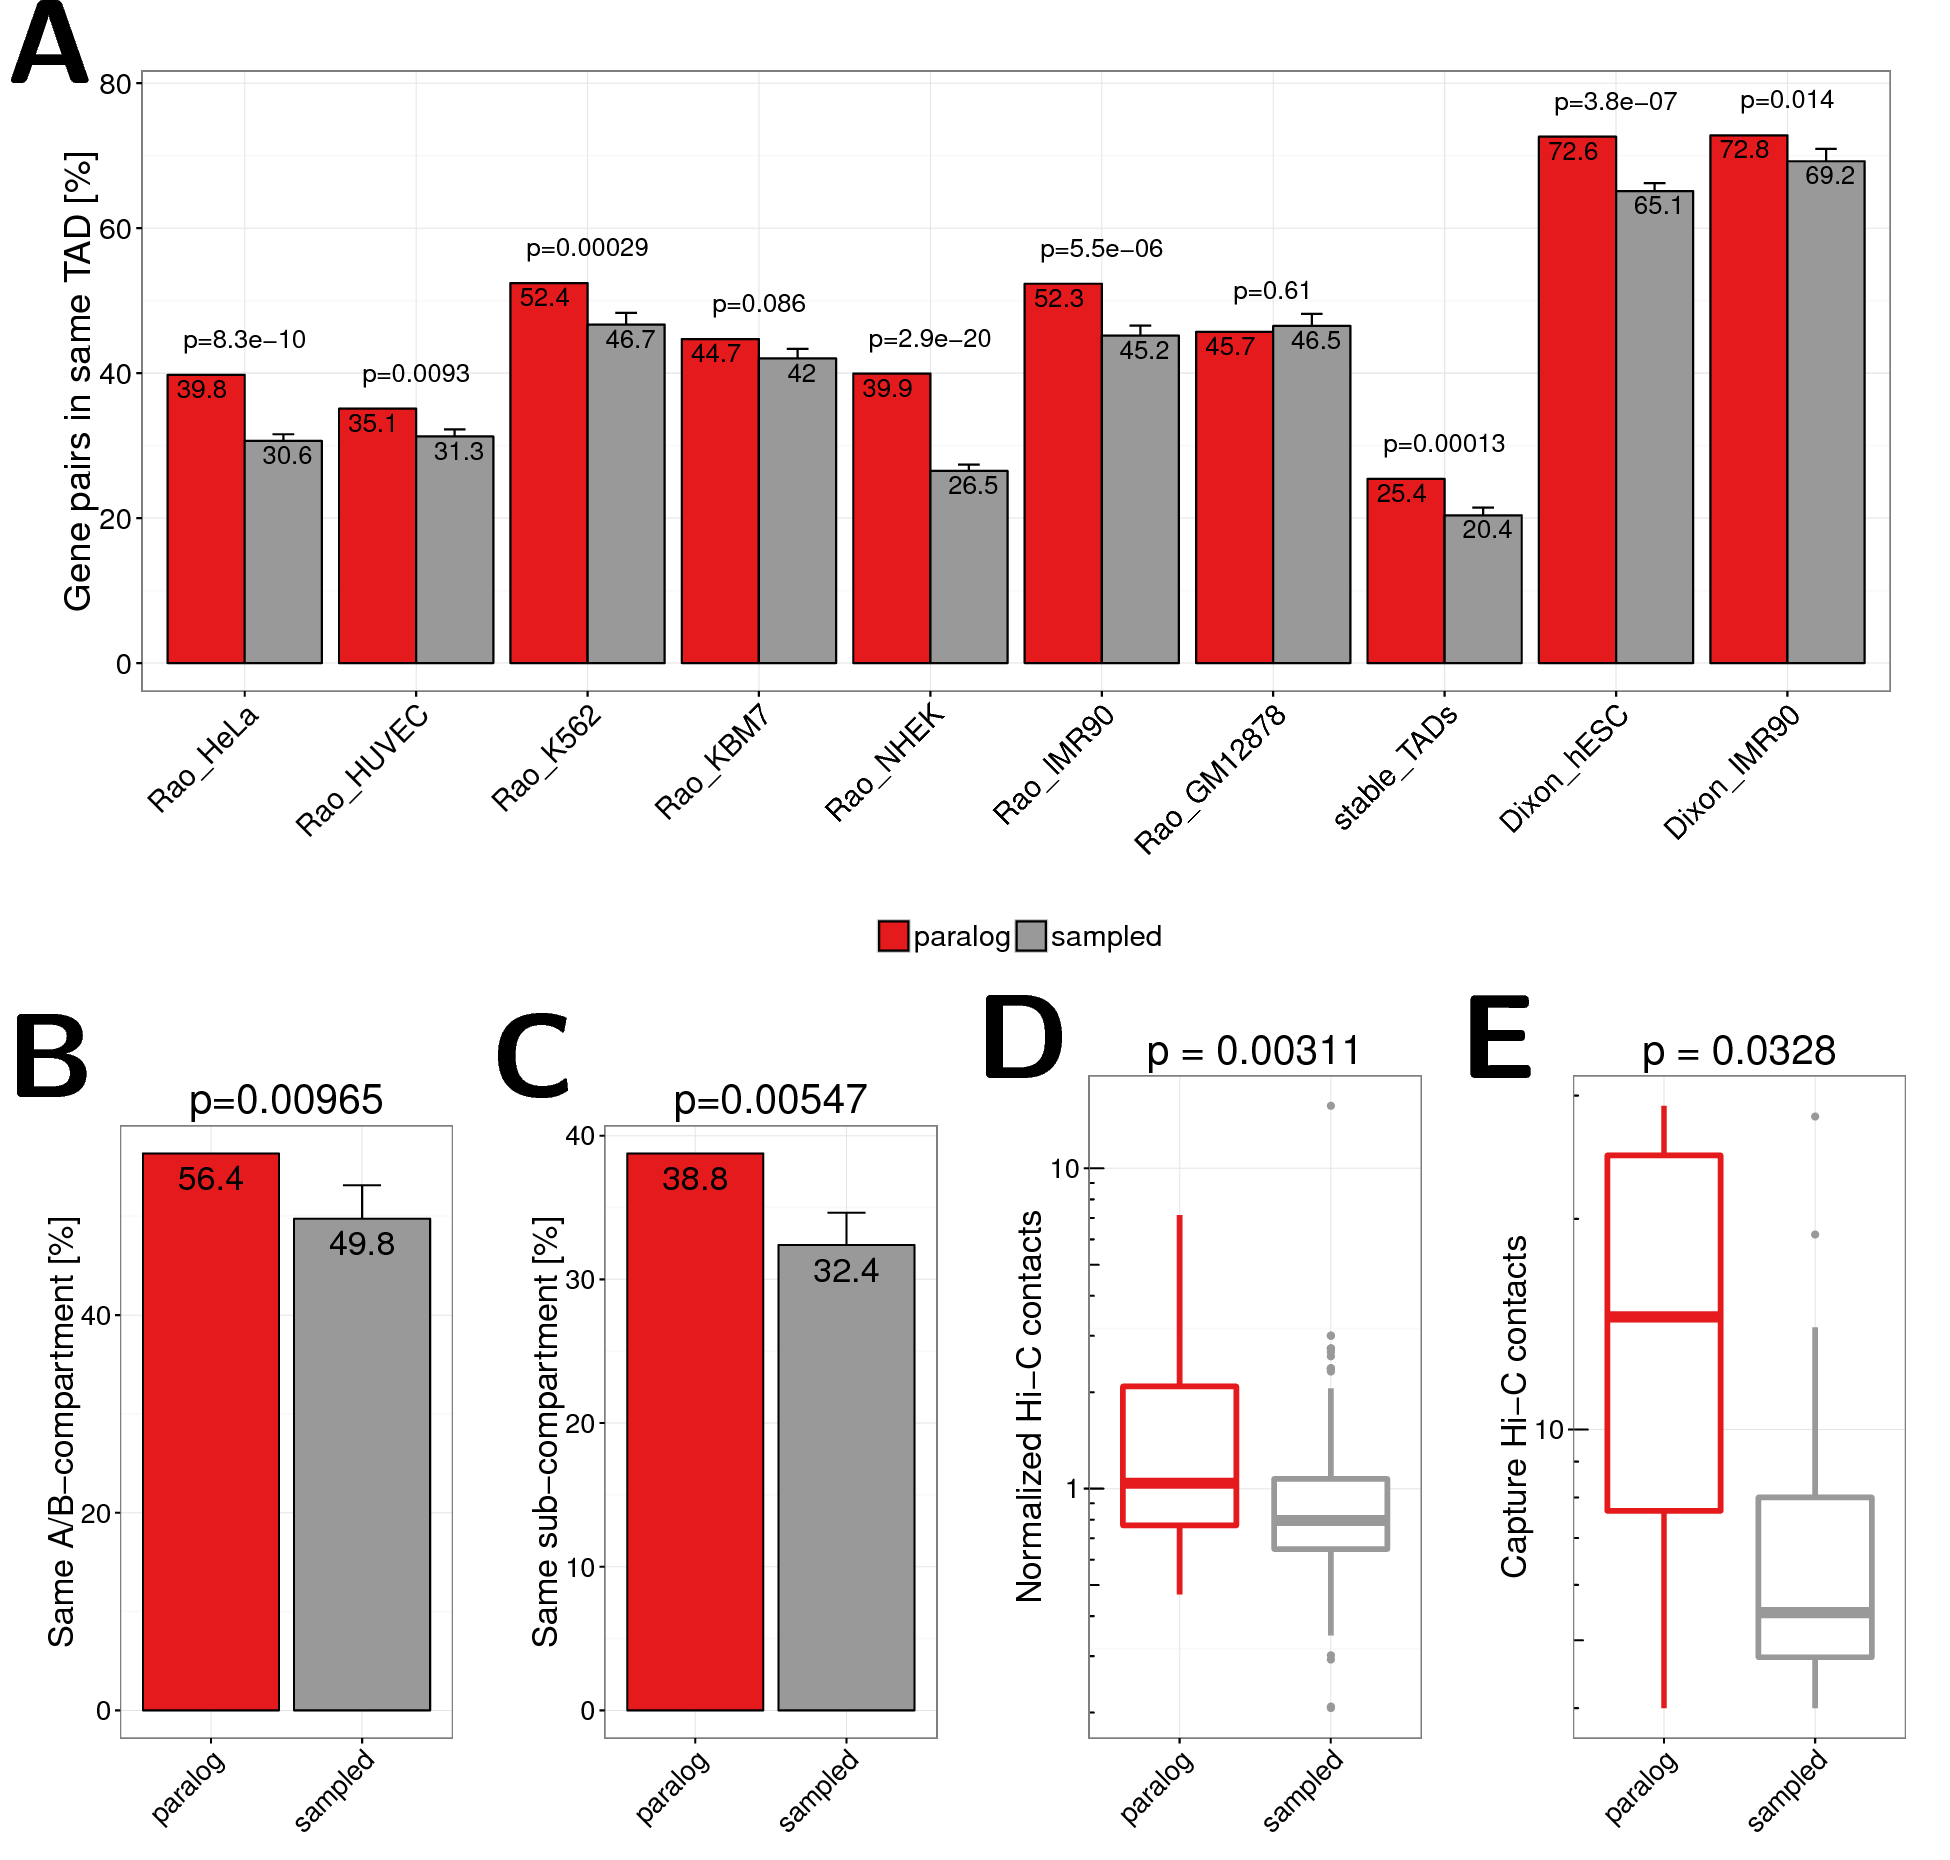
\includegraphics[width=0.5\linewidth]{figures/paralog/fig3_09} 

}

\caption{\textbf{(A)} Co-localization of close paralog genes within the
same TAD compared against sampled gene pairs for TAD data sets from
different cell types and studies. The first seven bars show values for
TADs called in HeLa, HUVEC, K562, KBM7, NHEK, IMR90, and GM12878 cells
by \citep{Rao2014}. The eighth bar shows the value for stable TADs
across cell types form this study (at least 90\% reciprocal overlap in
50\% of cells). The last two bars show data for TADs called in hESC and
IMR90 cells by \citep{Dixon2012}. Error bars indicate standard deviation
in 10 times replicated sampling of gene pairs. P-values are computed
using Fisher's exact test. \textbf{(B)} Percent of gene pairs annotated
to same A/B compartment according to Hi-C data in GM12878 cells from
\citep{Rao2014}. Pairs located in the very same compartment interval
were excluded. \textbf{(C)} Percent of gene pairs annotated to same sub
compartment (A1, A2, B1, B2, B3, B4) according to \citep{Rao2014}. Pairs
located in the same subcompartment interval were excluded. \textbf{(D)}
Normalized Hi-C contact frequencies between TSSs of distal paralog gene
pairs and sampled background gene pairs. \textbf{(E)} Promoter capture-C
contact frequencies between distal paralog gene pairs and sampled
background gene pairs.}\label{fig:TAD}
\end{figure}





















Beside TADs, Hi-C interaction maps have revealed interaction patterns of
two compartments (A and B) that alternate along chromosomes in intervals
of several Mb. Thereby loci in A compartment preferentially associate
with other loci in A and loci in B with others in
B~\citep{Lieberman-Aiden2009, Rao2014, Dekker2013}. We therefore asked
whether pairs of paralogs from the same chromosome are preferentially
located within the same compartment (both A or both B) whereby we
excluded pairs that are in the same compartment interval. We found that
\(56.4\%\) of paralogs on the same chromosome but not in the same
compartment interval are in compartments of the same type. This was only
observed for \(49.2\%\) of sampled pairs (\(p=0.0046\),
Fig.~\ref{fig:TAD}B). Next we tested the same for recently distinguished
sub-compartment types from high-resolution Hi-C interaction
maps~\citep{Rao2014}. Again, paralogs are enriched to be located within
the same sub-compartment type (\(38.9\%\) vs. \(31.6\%\), \(p=0.0046\),
Fig.~\ref{fig:TAD}C).

These results show that close paralogs are enriched to be located in the
same regulatory unit of the genome as defined both by TADs and
compartments.

\subsection{Distal paralog pairs are enriched for long-range chromatin
contacts}\label{distal-paralog-pairs-are-enriched-for-long-range-chromatin-contacts}

Since it was shown that actively transcribed genes are localized in the
same active spatial compartments and tend to contact each other
frequently in the nucleus (at their
promoters~\citep{Cremer2015, Mifsud2015}) we hypothesised that this
might be the case for distal paralogs on the same chromosome too. As
spatial proximity can be approximated by Hi-C contact
frequencies~\citep{Lieberman-Aiden2009} we compared the number of
normalized Hi-C contacts between TSS of distal paralog genes (that have
promoters separated by more than 1 Mb) to the sampled gene pairs with
the same linear distances distribution. We used recently published in
situ Hi-C data from IMR90 cells at 5kb bin-size
resolution~\citep{Rao2014} and observed significantly more normalized
chromatin interactions between paralog genes compared to sampled control
gene pairs (\(p=0.0022\), Fig.~\ref{fig:TAD}D). We furthermore used an
independent data set of high resolution promoter-promoter interactions
measured by capture Hi-C~\citep{Mifsud2015}. Again, we observed a strong
enrichment of promoter-promoter interactions between distal paralogs
compared to control genes pairs (\(p=0.027\), Fig.~\ref{fig:TAD}E). This
shows that also distal paralogs are enriched for long-range
interactions, indicating that they tend to be in closer spatial
proximity than other genes.

\subsection{Close paralogs have fewer contacts than
expected}\label{close-paralogs-have-fewer-contacts-than-expected}

The observed enrichment of Hi-C contacts of paralogs is distance
dependent. We observe for close paralogs fewer Hi-C contacts than for
equally distant sampled gene pairs (Fig.~\ref{fig:closePairs}A). To
analyse this in more detail we focused on only those pairs on the same
chromosome that have a TSS distance of at least 10kb but less than 1Mb.
This is the distance range of most paralog pairs and allows to separate
genes in Hi-C interaction maps and TADs
(Fig.~\ref{fig:closePairsInTAD}A). Consequently, we observe paralogs
more often in the same TAD in eight out of nine data sets for this
distance range (Fig.~\ref{fig:closePairsInTAD}B). For these pairs we
observe significant lower Hi-C contact frequencies if pairs are within
the same IMR90 TAD~\citep{Rao2014} as compared to sampled genes
(\(p=0.00094\)) but not if pairs are in different TADs (\(p=0.81\),
Fig.~\ref{fig:closePairs}B). We got comparable results when analysing
the Capture Hi-C data the same way (Fig.~\ref{fig:closePairsInTAD}C).
Next, we tested whether this can be explained by the nested sub-TAD
structure of TADs called from high-resolution Hi-C in
IMR90~\citep{Rao2014}. We divided pairs into four groups, namely, 'no
TAD', if both pairs are not in any TAD, 'different TAD', if pairs do not
have at least one TAD in common, 'different sub-TADs', if they have at
least one TAD in common but are in different sub-TADs, and 'same
sub-TAD', if they overlap exactly the same set of TADs. While we saw
that paralogs are more often in the no TAD group
(\(p=1.4\times10^{-20}\)), we found that they were highly depleted from
the different TAD group (\(p=1.6\times10^{-40}\)) and highly enriched to
be located within the same sub-TAD (\(p=4.2\times10^{-9}\),
Fig.~\ref{fig:closePairs}C). However, although not always significant,
paralogs have fewer Hi-C contacts than sampled gene pairs in all of
these groups (Fig.~\ref{fig:closePairs}D). In addition, close paralogs
within the same TAD share more enhancers than close paralogs not being
in the same TAD (Fig.~\ref{fig:closePairs}E). However, the positive
correlation of gene expression over different tissues is not
significantly higher for paralogs whether they are in the same TAD or
not (Fig.~\ref{fig:ExpByTAD}).

\begin{figure}

{\centering 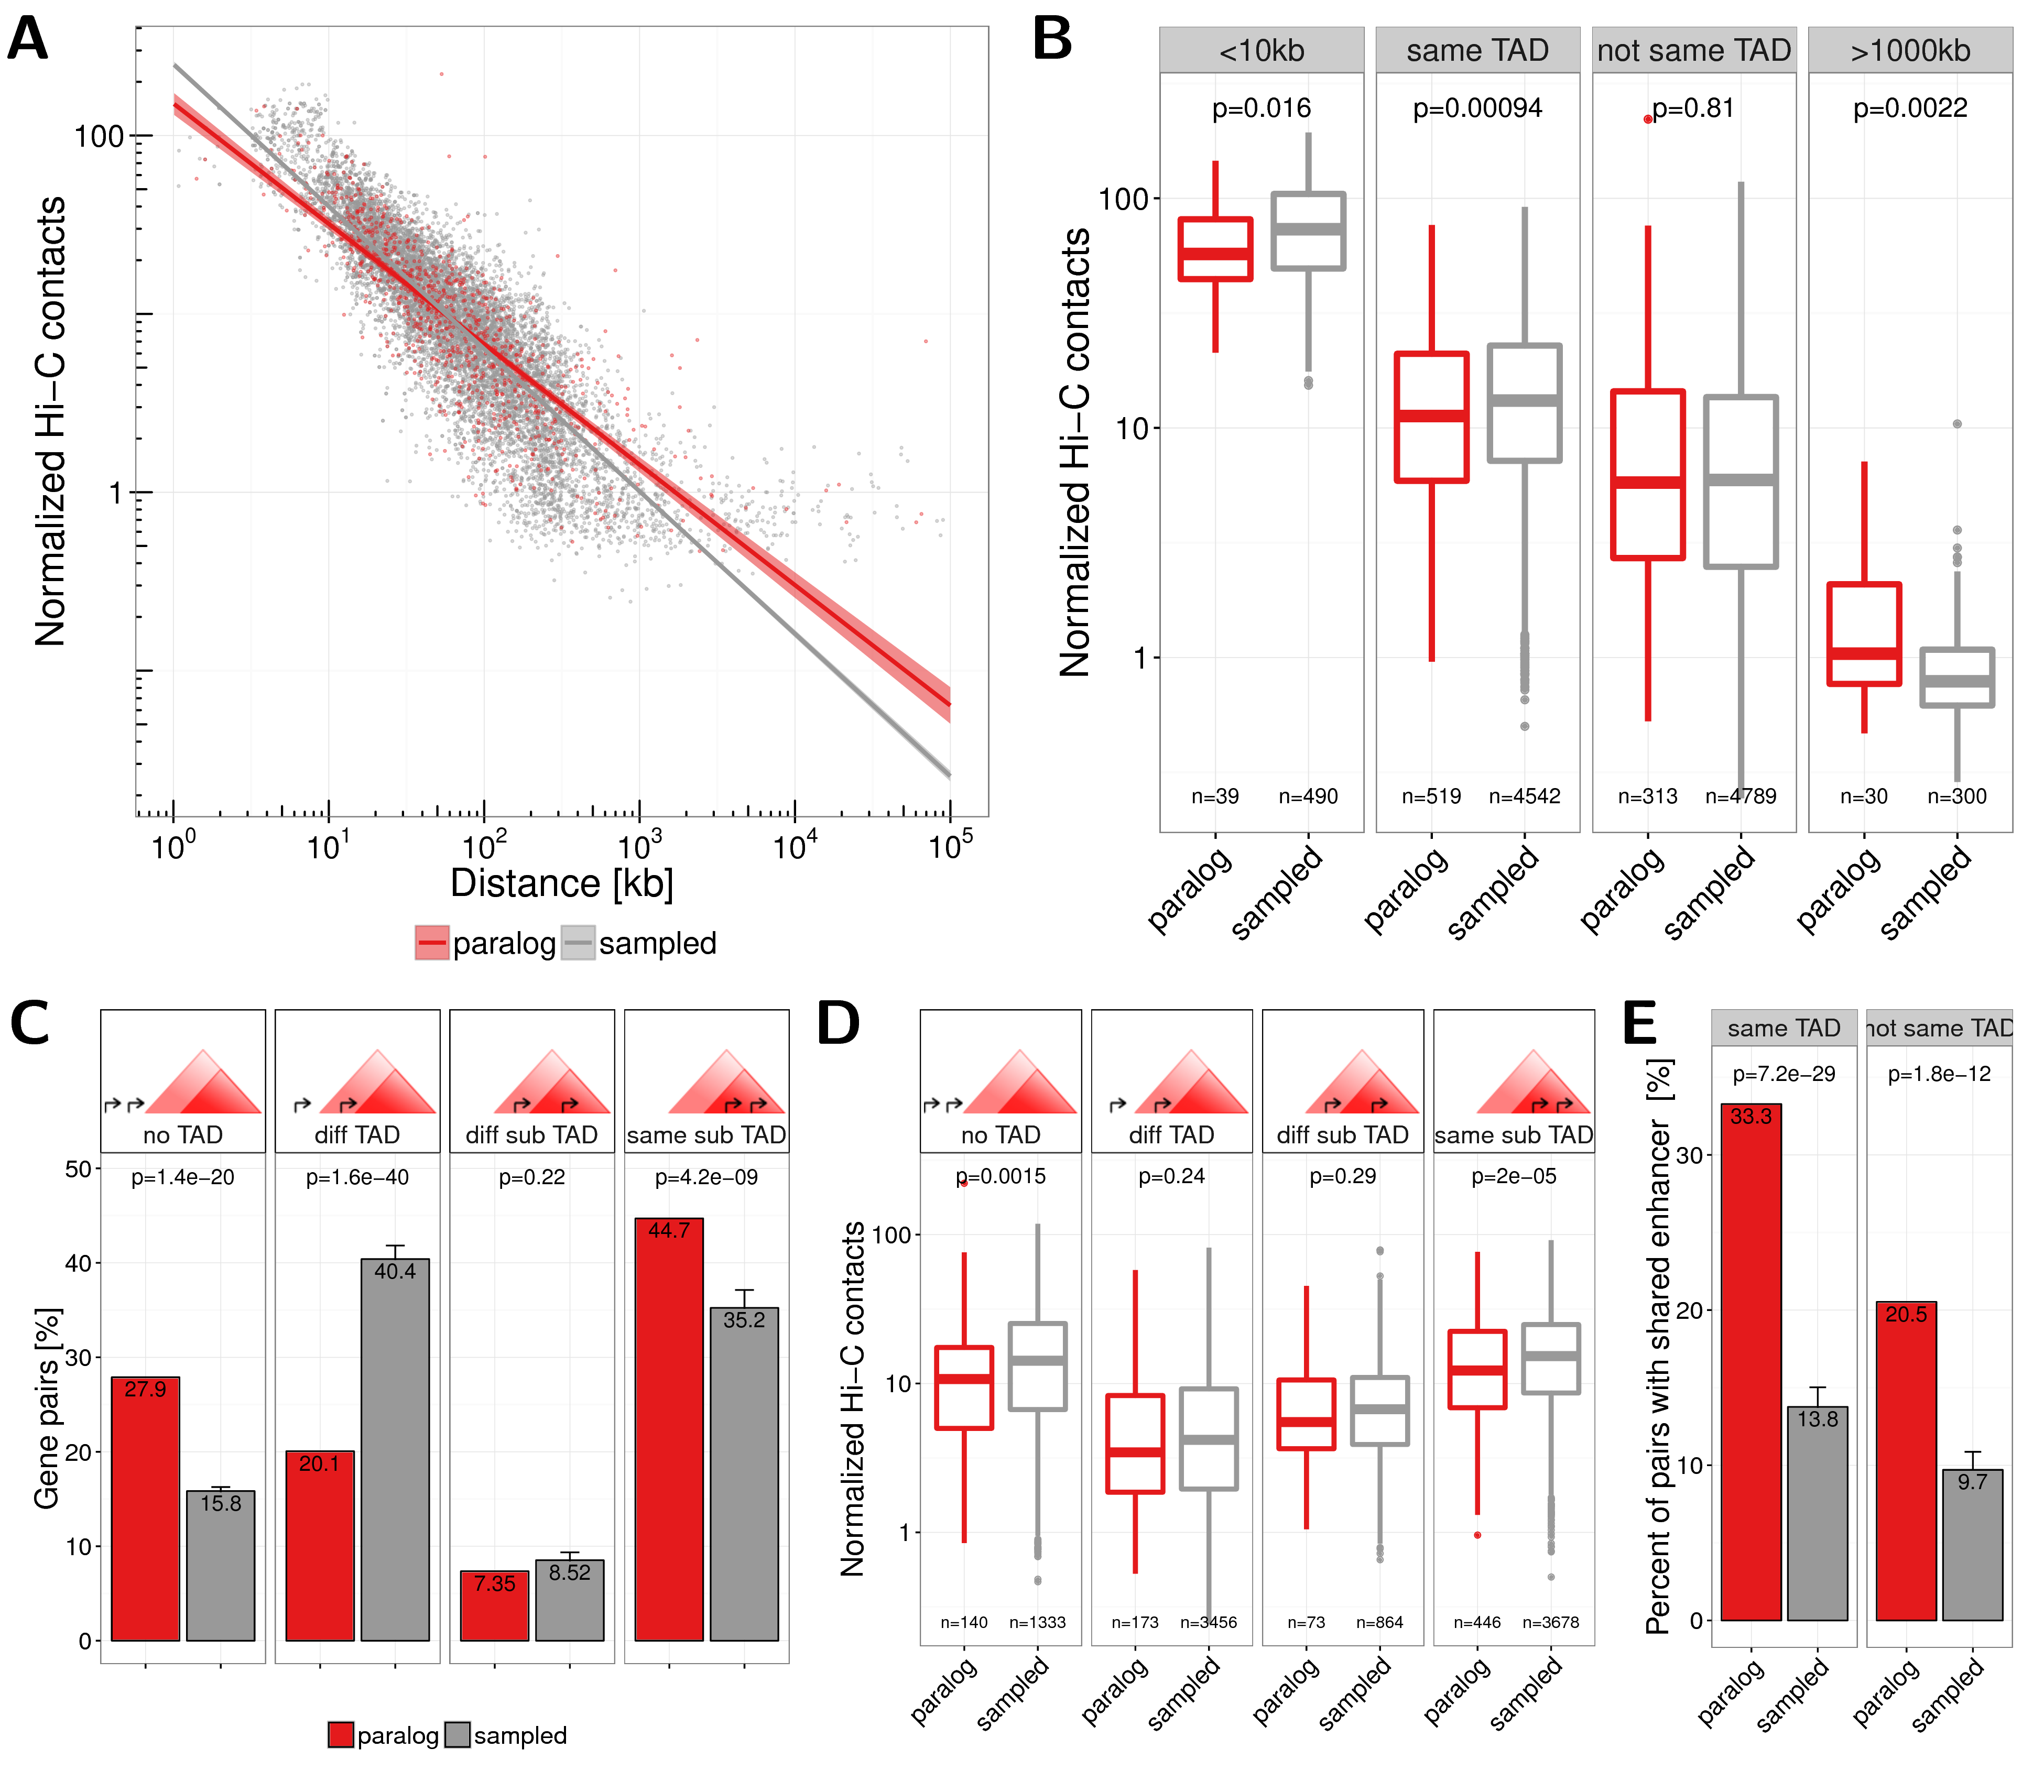
\includegraphics[width=0.5\linewidth]{figures/paralog/fig4_09} 

}

\caption{\textbf{(A)} Normalized Hi-C contacts by genomic
distance between paralog (red) and sampled (grey) gene pairs. Lines show
linear regression fit separately for paralogs (red) and sampled (grey)
pairs with 95\% confidence intervals in shaded areas. \textbf{(B)}
Normalized Hi-C contacts between pairs of paralogs (red) and sampled
gene pairs (grey) for the groups: \$\textless{}\$10kb genomic distance,
located in the same TAD, not in the same TAD, and with genomic distance
\$\textgreater{}\$1000kb. \textbf{(C)} Number of gene pairs located
either in no TAD, in different TADs (or only one pair member in a TAD),
both in a TAD but in different sub-TADs, or within the same sub-TAD, for
paralogs (red) and sampled (grey) pairs. TADs from IMR90 cells from
\citep{Rao2014} were used, which nested in contrast to TAD calls from
\citep{Dixon2012}. \textbf{(D)} Normalized Hi-C contacts between pairs
of paralogs (red) and sampled gene pairs (grey) for the four groups of
pairs in sub-TAD structures shown in (C). \textbf{(E)} Percent of gene
pairs with at least one shared enhancer for paralog genes (red) and
sampled control genes (grey) separated for pairs in the same IMR90 TAD
(left) or not (right).}\label{fig:closePairs}
\end{figure}




















In summary, we observed that while close paralogs (situated at less than
1Mb) have more shared enhancers if they are in the same TAD than not,
these within TAD paralog pairs have fewer contacts compared to other
within TAD pairs of genes.

\subsection{Paralogs in mouse and dog
genome}\label{paralogs-in-mouse-and-dog-genome}

Next, we asked whether the co-localization and co-regulation of paralogs
is conserved in other species. For this, we conducted an analogous
analysis with paralog gene pairs from mouse (\emph{M. musculus}) and dog
(\emph{C. familaris}) genomes. Similar as for human data, we found that
more than two third of the genes had at least one paralog copy
(Fig.~\ref{fig:paralogsSpecies}A,D), paralog pairs clustered on the same
chromosome (Fig.~\ref{fig:paralogsSpecies}B,E), and had close linear
distances (Fig.~\ref{fig:paralogsSpecies}C,F).

We sampled control gene pairs with the same distance distribution as
paralogs for both species separately
(Fig.~\ref{fig:paralogsSpecies}C,F). We used TADs from recently
published Hi-C data in liver cells of mouse and
dog~\citep{VietriRudan2015}, which have a size distribution comparable
to TADs from human cells (Fig.~\ref{fig:TADsize}). We computed the
fraction of paralog pairs that are located in the same TAD for both
species. Consistent with the observation in human, we found that
paralogs tend to colocalize more frequently within the same TAD in mouse
(\(p=7.2 \times 10^{-22}\)) and dog (\(p=0.00064\)) than expected by
chance (Fig.~\ref{fig:paralogsMouseDog}A). We also quantified directly
the contact frequencies between promoters of distal paralogs on the same
chromosome and found them significantly more frequently in contact than
sampled gene pairs with the same genomic distance for paralogs in mouse
(\(p=7\times 10^{-7}\)) and dog (\(p=0.008\))
(Fig.~\ref{fig:paralogsMouseDog}B). Together, these results indicate
that enriched long-range interactions between paralogs are not human
specific but rather a general evolutionary conserved feature of genome
organization.

\begin{figure}

{\centering 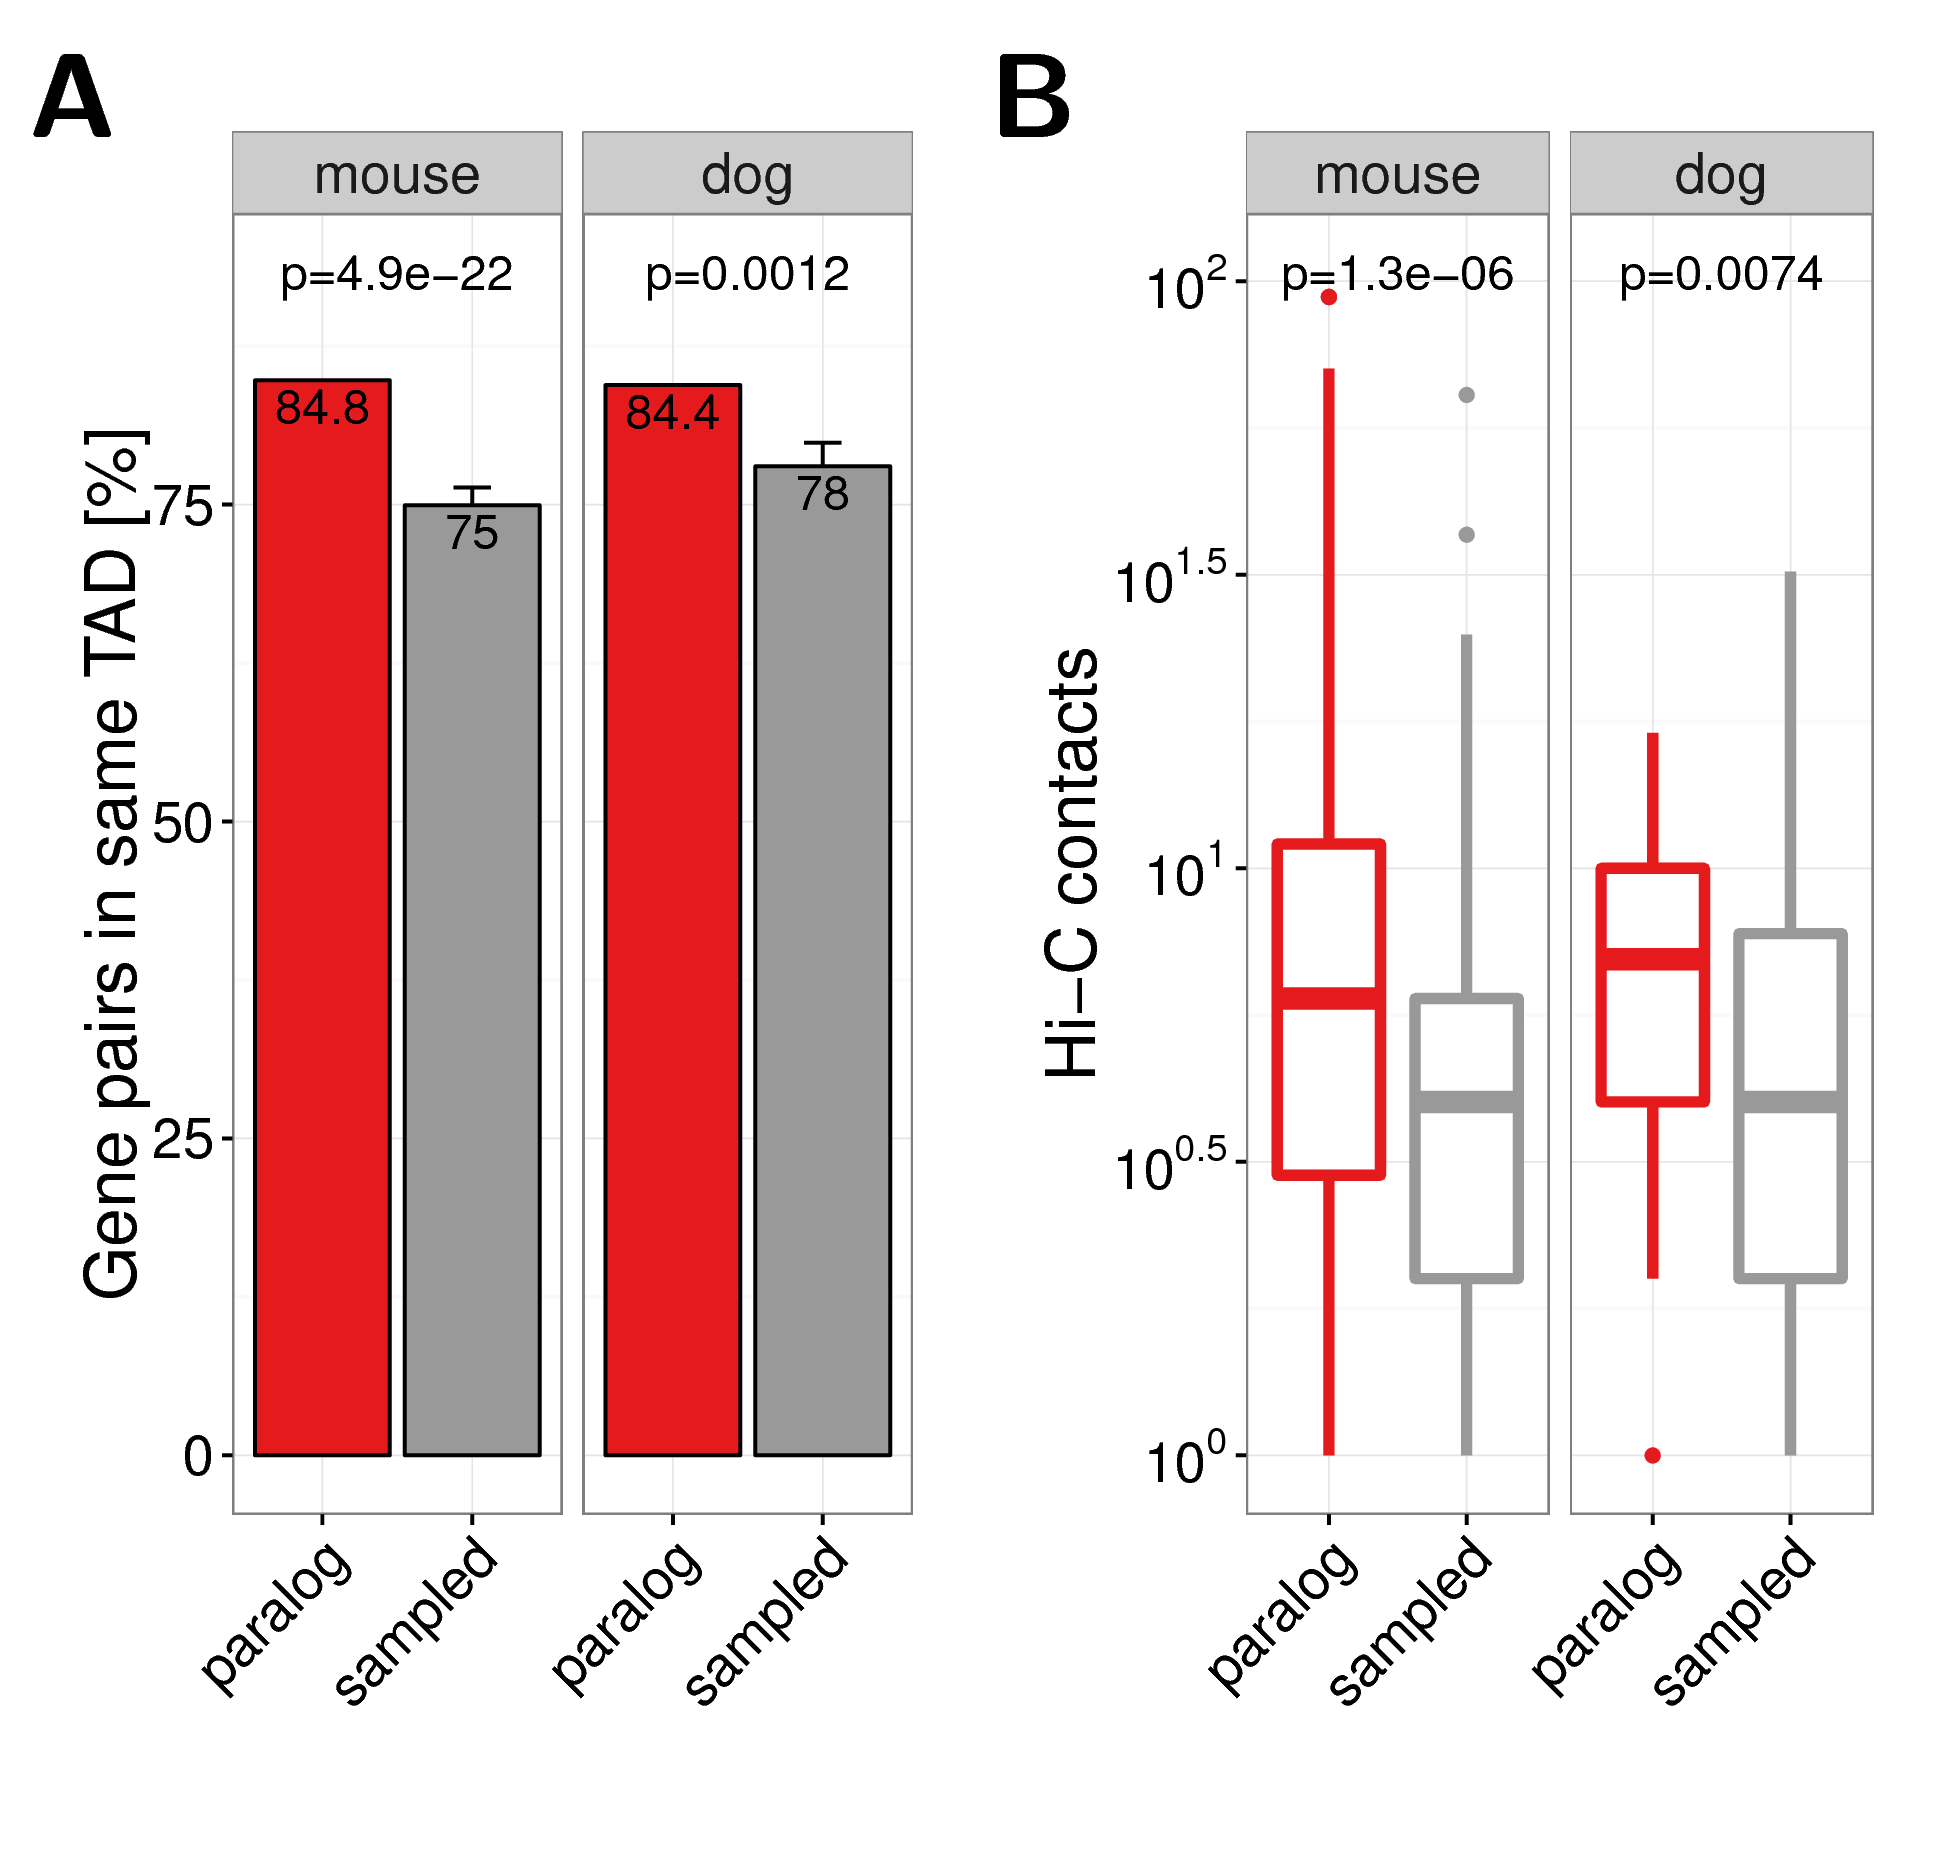
\includegraphics[width=0.5\linewidth]{figures/paralog/fig5_09} 

}

\caption{\textbf{(A)} Co-occurrence of close paralog genes
with the same TAD in mouse (left panel) and dog (right panel).
\textbf{(B)} Hi-C contacts between promoter of distal gene pairs in Hi-C
experiments in liver cells from mouse (left panel) and dog (right
panel). Hi-C data and TAD calls were taken from \citep{VietriRudan2015}.}\label{fig:paralogsMouseDog}
\end{figure}







\subsection{Orthologs of human paralogs show conserved
co-localization}\label{orthologs-of-human-paralogs-show-conserved-co-localization}

Next, we wanted to test more directly whether the spatial
co-localization of human paralogs is indeed conserved during evolution.
In cases where the gene duplication event occurred before the separation
of human and mouse (or human and dog) we can eventually assign each
human gene of a pair of paralogs to one ortholog in mouse (or dog
genomes) (Fig.~\ref{fig:orthologModel}).

We could map \(37.1\%\) (\(n=579\)) and \(34.6\%\) (\(n=540\)) of the
close human paralogs to one-to-one orthologs in mouse and dog,
respectively (Fig.~\ref{fig:orthologsSpecies}A,D). We hypothesised that
the two one-to-one orthologs of human paralog pairs would also be close
in the mouse and dog genomes. Indeed, we found that the orthologs of
human paralogs tend to cluster on the same chromosome
(Fig.~\ref{fig:orthologsSpecies}B,E) and are biased for close linear
distances (Fig.~\ref{fig:orthologsSpecies}C,F).

We further investigated how many one-to-one orthologs of the human
paralog pairs were located in the same TAD in mouse and dog genomes.
Although not significant, we found that mouse orthologs of close human
paralogs share more often the same TAD in mouse than orthologs of
sampled human gene pairs (\(80\%\) vs. \(76\%\), \(p=0.11\);
Fig.~\ref{fig:orthologsMouseDog}A). Significant enrichment was observed
with orthologs in the dog genome (\(85\%\) vs. \(77\%\), \(p=0.0016\);
Fig.~\ref{fig:orthologsMouseDog}A).

\begin{figure}

{\centering 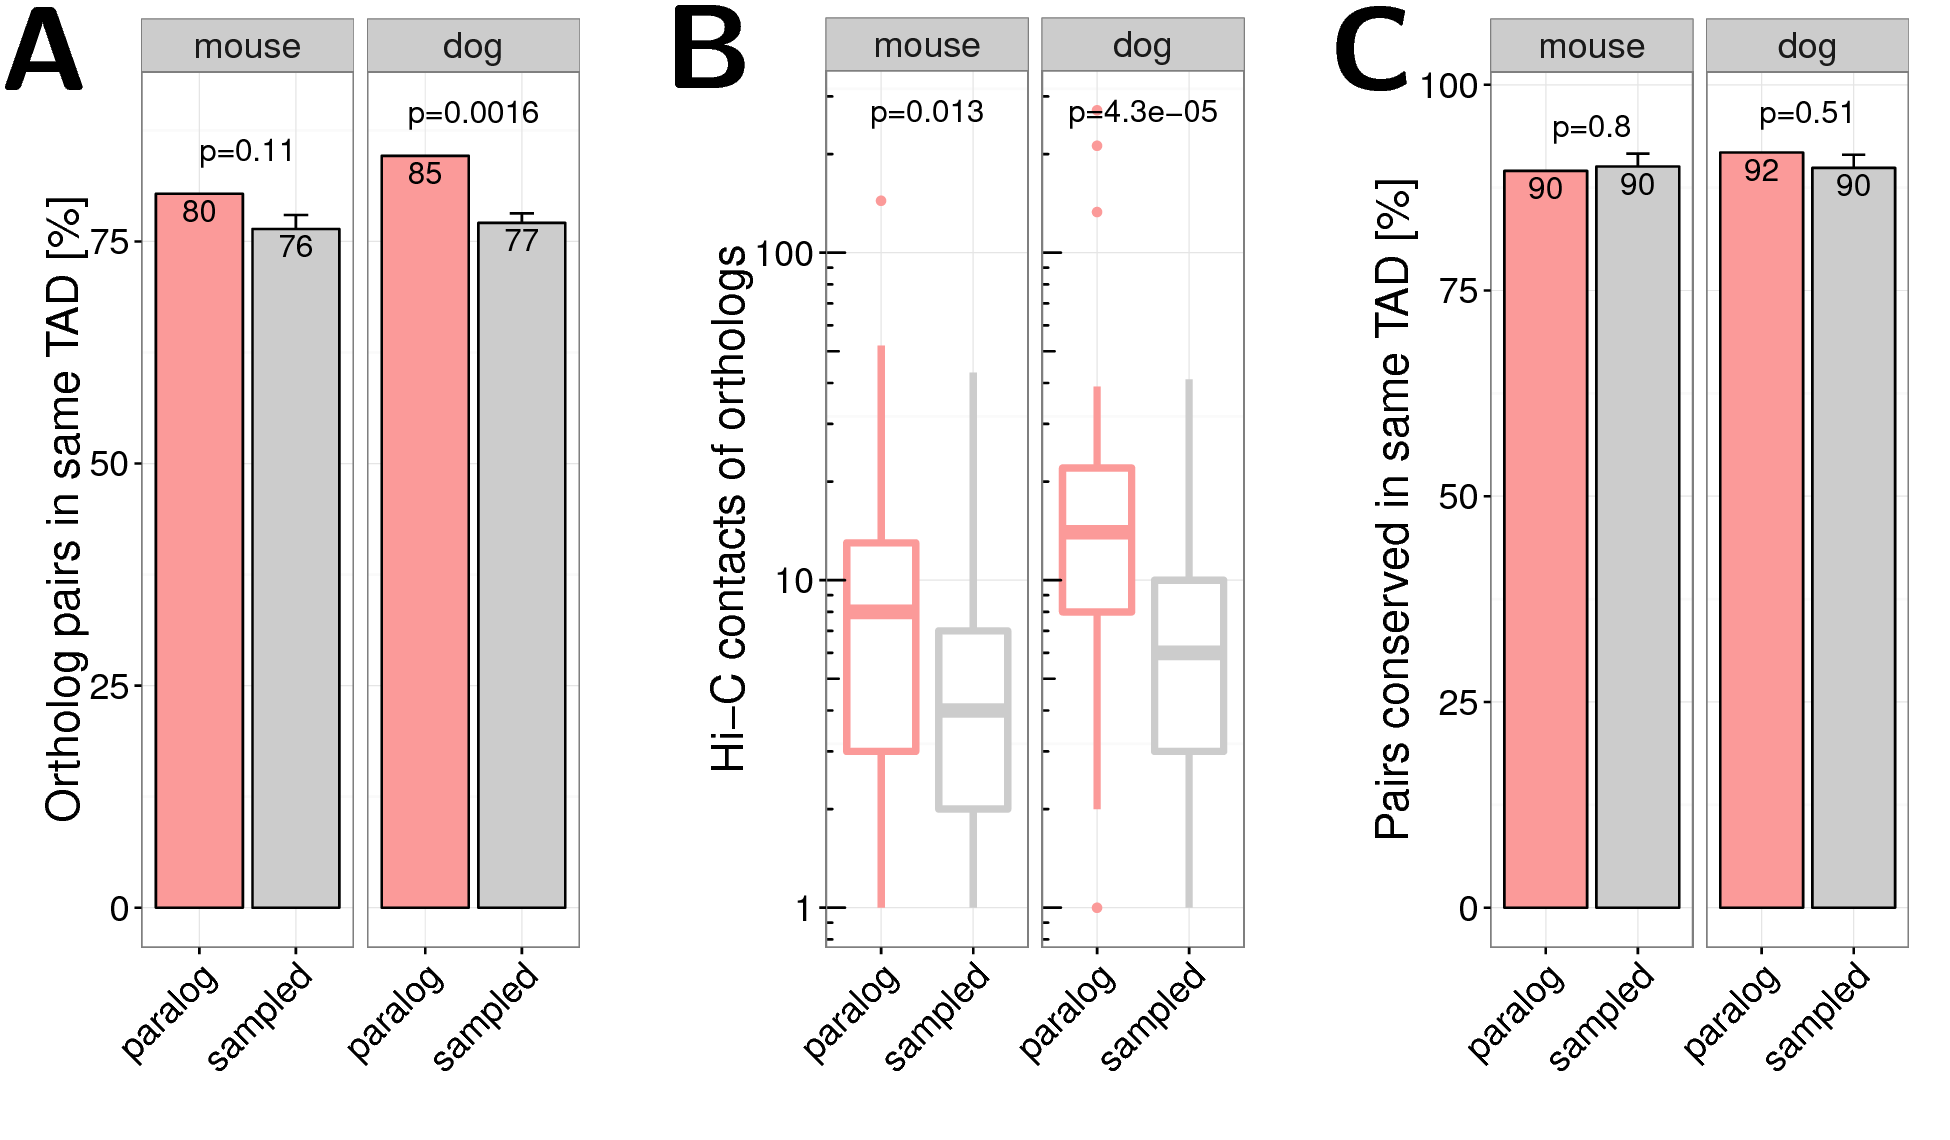
\includegraphics[width=0.5\linewidth]{figures/paralog/fig6_09} 

}

\caption{One-to-one orthologs of human paralog genes in
mouse and dog genome. \textbf{(A)} Percent of mouse (left) and dog
(right) orthologs of human paralog pairs that are in the same TAD in the
mouse and dog genome, respectively. \textbf{(B)} Normalized Hi-C
contacts between promoters of one-to-one orthologs of human distal
paralogs in the mouse (left) and dog (right) genome. \textbf{(C)}
Percent of gene pairs with conserved co-localization. Orthologs in the
same TAD in mouse (left) and dog (right) as percent of all orthologs of
human paralog pairs that are in the same TAD in human. For human TADs
from IMR90 cells from \citep{Rao2014} were used.}\label{fig:orthologsMouseDog}
\end{figure}












For distal human paralogs we quantified the promoter contacts of their
orthologs in mouse and dog and found enriched Hi-C contacts in mouse
(\(p=0.011\)) and dog (\(p=2.4\times 10^{-5}\);
Fig.~\ref{fig:orthologsMouseDog}B).

These results show that both the co-localization of paralogs in TADs and
the contacts between distal paralogs are only weekly conserved at the
evolutionary distances examined here. For example, we see that given a
pair of human genes in the same TAD the likelihood of their orthologs
being in the same TAD in mouse or dog is the same whether they are
paralogs or not (Fig.~\ref{fig:orthologsMouseDog}C).

All together, our results support the notion that tandem duplications
generate paralog gene pairs that are selected if they accommodate in
TADs but following evolutionary events allow their reorganization
outside TADs. While within oganisms distal paralog genes are
coordinated, such coordination can be eventually erased by evolution.

\section{DISCUSSION}\label{discussion}

The generation of large datasets of gene expression across multiple
tissues allowed the observation of clusters of pairs and triplets of
co-expressed genes in higher eukaryotes (e.g.~in
\emph{Drosophila}~\citep{Boutanaev2002} or in
mammals~\citep{Purmann2007}) and it was previously suspected that the
structure of chromatin would have to do with this~\citep{Sproul2005},
particularly cis-acting units~\citep{Purmann2007}. The discovery and
characterization of topologically associating domains (TADs) has finally
brought to the light the chromatin structure that could be responsible
for this co-regulation.

To study the interplay between TADs, gene co-regulation and evolution in
the human genome, we decided to focus on pairs of paralogs because they
have a tendency to be produced by tandem duplication~\citep{Newman2015}
and, because of homology, result in proteins with related functions.
However, the particular emergence and evolution of paralogs are probably
responsible for special properties that distinguish them from
non-paralog genes as we described: greater gene length, more enhancers,
as well as a shorter distance to the next enhancer. These differences,
which could be partially explained by the observation that paralogs are
more often tissue specific (Fig.~\ref{fig:paraVSnonPara}F), complicated
the methodology for choosing meaningful control pairs (see section
\ref{sec:paralog-methods}).

Once we ensured the generation of the appropriate backgrounds, we could
study the position of pairs of paralogs respect to TADs. This allowed us
to test, on the one hand, the resilience of TADs to genome shuffling
and, on the other hand, the rate of accommodation and gain of
functionally related genes. Possibly, the generation of paralogs by
tandem duplication might continuously impose a strain in the
pre-existing genomic and regulatory structure, but also a chance for the
evolution of new functionality.

On the one hand, we observed many pairs of paralogs within TADs. On the
other hand, pairs of paralogs in different TADs, however distant from
each other, tend to have more contacts than control gene pairs. This
suggests a many-step mechanism where first tandem duplication fits TAD
structure but then subsequent chromosomal rearrangements relocate
paralogs at larger distances (while keeping contacts) and eventually
reorganization of regulatory control allow their increased independence
being eventually placed even in different chromosomes where contact is
no longer necessary. Thus, TADs are units of co-regulation but do not
have a strong preference for keeping co-regulated genes within during
evolution. This model agrees with the recent work from Lan and Pritchard
reporting that young pairs of paralogs are generally close in the
genome~\citep{Lan2016}.

A second effect that we observed was the existence of fewer contacts
between close pairs of paralogs than in comparable pairs of non-paralog
genes, particularly if they are in the same TAD
(Fig.~\ref{fig:closePairs}B), while sharing more enhancers
(Fig.~\ref{fig:closePairs}E). This result could reflect the existence of
pairs of paralogs encoding proteins that replace each other, for example
sub-units of a complex that occupy the same position in a protein
complex but are expressed in different cells. One such case is
exemplified by CBX2, CBX4 and CBX8, which occupy neighbouring positions
within the same TAD in human chromosome 17 and encode replaceable
subunits of the polycomb repressive complex 1 (PRC1) complex involved in
epigenetic regulation of cell specification~\citep{Becker2015}. The
expression of such groups of paralogs require active coordination to
ensure exclusive expression of only one gene or a subset of genes per
condition, resulting in patterns of divergent expression. Since there
might be also conditions where none of these genes are expressed, such
divergent expression patterns are different from negative correlation.

Previous work studying gene expression of duplicated genes already
studied how after gene duplication paralogs tend to diverge in their
expression \citep{Makova2003, Huminiecki2004, Rogozin2014} but it was
observed that while some paralogs are co-expressed some others have
negative correlation across tissues \citep{Makova2003}. Our
interpretation of these observations together with our results is that
the initial tandem duplication event forming a paralog is advantageous
to situate the new copy in an environment that allows its controlled
regulation, ideally under the same regulatory elements than the original
copy, and this can be attained by duplicating both gene and surrounding
regulatory elements. This would preclude the duplication of genes with
very entangled regulatory associations. Once this happens, if the new
protein evolves into a replacement, then the regulatory constraints on
its coding gene are strong and there would be a tendency to keep it in
the vicinity of the older gene so that a divergent pattern of expression
can be ensured.

To support this hypothesis, we contrasted our data with the data
collected in the HIPPIE database of experimentally verified human
protein-protein interactions~\citep{Schaefer2012}. We observed the
well-known fact that paralog pairs generally encode for proteins that
interact more often than non-paralog proteins (Fig.~\ref{fig:PPI}). But,
most importantly, we observed that the chances of close pairs of genes
to encode for interacting proteins raise \(2.3\)-fold if they are in the
same TAD, while, in contrast, if these genes are paralogs the difference
is much smaller (\(1.2\)-fold, Fig.~\ref{fig:PPI}). We interpret this
result as evidence for a significant population of within TAD paralog
pairs encoding for non-interacting proteins, which supports our
hypothesis that paralog pairs within the same TAD would have a tendency
to encode for proteins replacing each other.

\section{CONCLUSION}\label{conclusion}

We propose that paralog genes generated by tandem duplication start
their life coregulated within TADs, then are moved outside to other
places in the chromosome and eventually to different chromosomes. TADs
would then fit genomic duplications situating the new copy in a
duplicated regulatory enviroment. Subsequent genomic rearrangements
would create divergent regulatory circuits eventually allowing their
disentanglement. An exception would be genes that precise to be strongly
co-regulated with the original copy, for example, to produce a
replacement protein.

TADs would thus act as protective nests for evolving newcomer genes.
This seems to be a reasonable evolutionary mechanism, much simpler than
creating from nothing a complete new regulatory environment for a new
gene.

\section{ACKNOWLEDGEMENTS}\label{acknowledgements}

The authors thank all members of the CBDM group for fruitful
discussions.

\hypertarget{ch:TAD_evolution}{\chapter{Stability of TADs in
evolution}\label{ch:TAD_evolution}}

Evolutionary stability of topologically associating domains is
associated with conserved gene regulation

Jan Krefting\textsuperscript{1,2}, Miguel A.
Andrade-Navarro\textsuperscript{1,2} and Jonas
Ibn-Salem\textsuperscript{1,2,\#}

\textsuperscript{1}Faculty of Biology, Johannes Gutenberg University of
Mainz, 55128 Mainz, Germany

\textsuperscript{2}Institute of Molecular Biology, 55128 Mainz, Germany

\# corresponding author

\url{https://doi.org/10.1101/231431}

\subsection*{Abstract}\label{abstract}
\addcontentsline{toc}{subsection}{Abstract}

\textbf{Background:} The human genome is highly organized in the
three-dimensional nucleus. Chromosomes fold locally into topologically
associating domains (TADs) defined by increased intra-domain chromatin
contacts. TADs contribute to gene regulation by restricting chromatin
interactions of regulatory sequences, such as enhancers, with their
target genes. Disruption of TADs can result in altered gene expression
and is associated to genetic diseases and cancers. However, it is not
clear to which extent TAD regions are conserved in evolution and whether
disruption of TADs by evolutionary rearrangements can alter gene
expression.

\textbf{Results:} Here, we hypothesize that TADs represent essential
functional units of genomes, which are selected against rearrangements
during evolution. We investigate this using whole-genome alignments to
identify evolutionary rearrangement breakpoints of different vertebrate
species. Rearrangement breakpoints are strongly enriched at TAD
boundaries and depleted within TADs across species. Furthermore, using
gene expression data across many tissues in mouse and human, we show
that genes within TADs have more conserved expression patterns.
Disruption of TADs by evolutionary rearrangements is associated with
changes in gene expression profiles, consistent with a functional role
of TADs in gene expression regulation.

\textbf{Conclusions:} Together, these results indicate that TADs are
conserved building blocks of genomes with regulatory functions that are
often reshuffled as a whole instead of being disrupted by
rearrangements.

\subsection*{Keywords}\label{keywords}
\addcontentsline{toc}{subsection}{Keywords}

Genome rearrangements; Topologically associating domains; TAD; Chromatin
interactions; 3D genome architecture; Hi-C; Evolution; Selection; Gene
regulation; Structural variants

\section{Introduction}\label{introduction-1}

The three-dimensional structure of eukaryotic genomes is organized in
many hierarchical levels \citep{Bonev2016}. The development of
high-throughput experiments to measure pairwise chromatin-chromatin
interactions, such as Hi-C \citep{Lieberman-Aiden2009} enabled the
identification of genomic domains of several hundred kilo-bases with
increased self-interaction frequencies, described as topologically
associating domains (TADs) \citep{Dixon2012, Nora2012}. Loci within TADs
contact each other more frequently and TAD boundaries insulate
interactions of loci in different TADs. TADs have also been shown to be
important for gene regulation by restricting the interaction of
cell-type specific enhancers with their target genes
\citep{Nora2012, Symmons2014, Zhan2017}. Several studies associated
disruption of TADs to ectopic regulation of important developmental
genes leading to genetic diseases \citep{Ibn-Salem2014, Lupianez2015}.
These properties of TADs suggested that they are functional genomic
units of gene regulation.

Interestingly, TADs are largely stable across cell-types
\citep{Dixon2012, Rao2014} and during differentiation \citep{Dixon2015}.
Moreover, while TADs were initially described for mammalian genomes, a
similar domain organization was found in the genomes of non-mammalian
species such as \emph{Drosophila} \citep{Sexton2012}, zebrafish
\citep{Gomez-Marin2015} \emph{Caenorhabditis elegans} \citep{Crane2015}
and yeast \citep{Hsieh2015, Mizuguchi2014}. Evolutionary conservation of
TADs together with their spatio-temporal stability within organisms,
would collectively imply that TADs are robust structures.

This motivated the first studies comparing TAD structures across
different species, which indeed suggested that individual TAD boundaries
are largely conserved along evolution. More than 54\% of TAD boundaries
in human cells occur at homologous positions in mouse genomes
\citep{Dixon2012}. Similarly, 45\% of contact domains called in mouse
B-lymphoblasts were also identified at homologous regions in human
lymphoblastoid cells \citep{Rao2014}. A single TAD boundary at the Six
gene loci could be traced back in evolution to the origin of
deuterostomes \citep{Gomez-Marin2015}. However, these analyses focused
only on the subset of syntenic regions that can be mapped uniquely
between genomes and do not investigate systematically if TAD regions as
a whole might be stable or disrupted by rearrangements during evolution.

A more recent study provided Hi-C interaction maps of liver cells for
four mammalian genomes \citep{VietriRudan2015}. Interestingly, they
described three examples of rearrangements between mouse and dog, which
all occurred at TAD boundaries. However, the rearrangements were
identified by ortholog gene adjacencies, which might be biased by gene
density. Furthermore, they did not report the total number of
rearrangements identified, leaving the question open of how many TADs
are actually conserved between organisms. It remains unclear to which
extent TADs are selected against disruptions during evolution
\citep{Nora2013}. All these studies underline the need to make a
systematic study to verify if and how TAD regions as a whole might be
stable or disrupted by rearrangements during evolution.

To address this issue we used whole-genome alignment data to analyze
systematically whether TADs represent conserved genomic structures that
are rather reshuffled as a whole than disrupted by rearrangements during
evolution. Furthermore, we used gene expression data from many tissues
in human and mouse to associate disruptions of TADs by evolutionary
rearrangements to changes in gene expression.

\section{Results}\label{results-1}

\subsection{Identification of evolutionary rearrangement breakpoints
from whole-genome
alignments}\label{identification-of-evolutionary-rearrangement-breakpoints-from-whole-genome-alignments}

To analyze the stability of TADs in evolution, we first identified
evolutionary rearrangements by using whole-genome alignment data from
the UCSC Genome Browser \citep{Kent2003, Kent2002} to compare the human
genome to 12 other species. These species where selected to have genome
assemblies of good quality and to span several hundred million years of
evolution. They range from chimpanzee to zebrafish
(Fig~\ref{fig:TadEvo1}). The whole-genome data consists of consecutive
alignment blocks that are chained and hierarchically ordered into
so-called net files as fills \citep{Kent2003}. To overcome alignment
artifacts and smaller local variations between genomes we only
considered top-level fills or non-syntenic fills and additionally
applied a size threshold to use only fills that are larger than 10 kb,
100 kb, or 1000 kb, respectively. Start and end coordinates of such
fills represent borders of syntenic regions and were extracted as
rearrangement breakpoints for further analysis (see Methods for
details).

\begin{figure}

{\centering 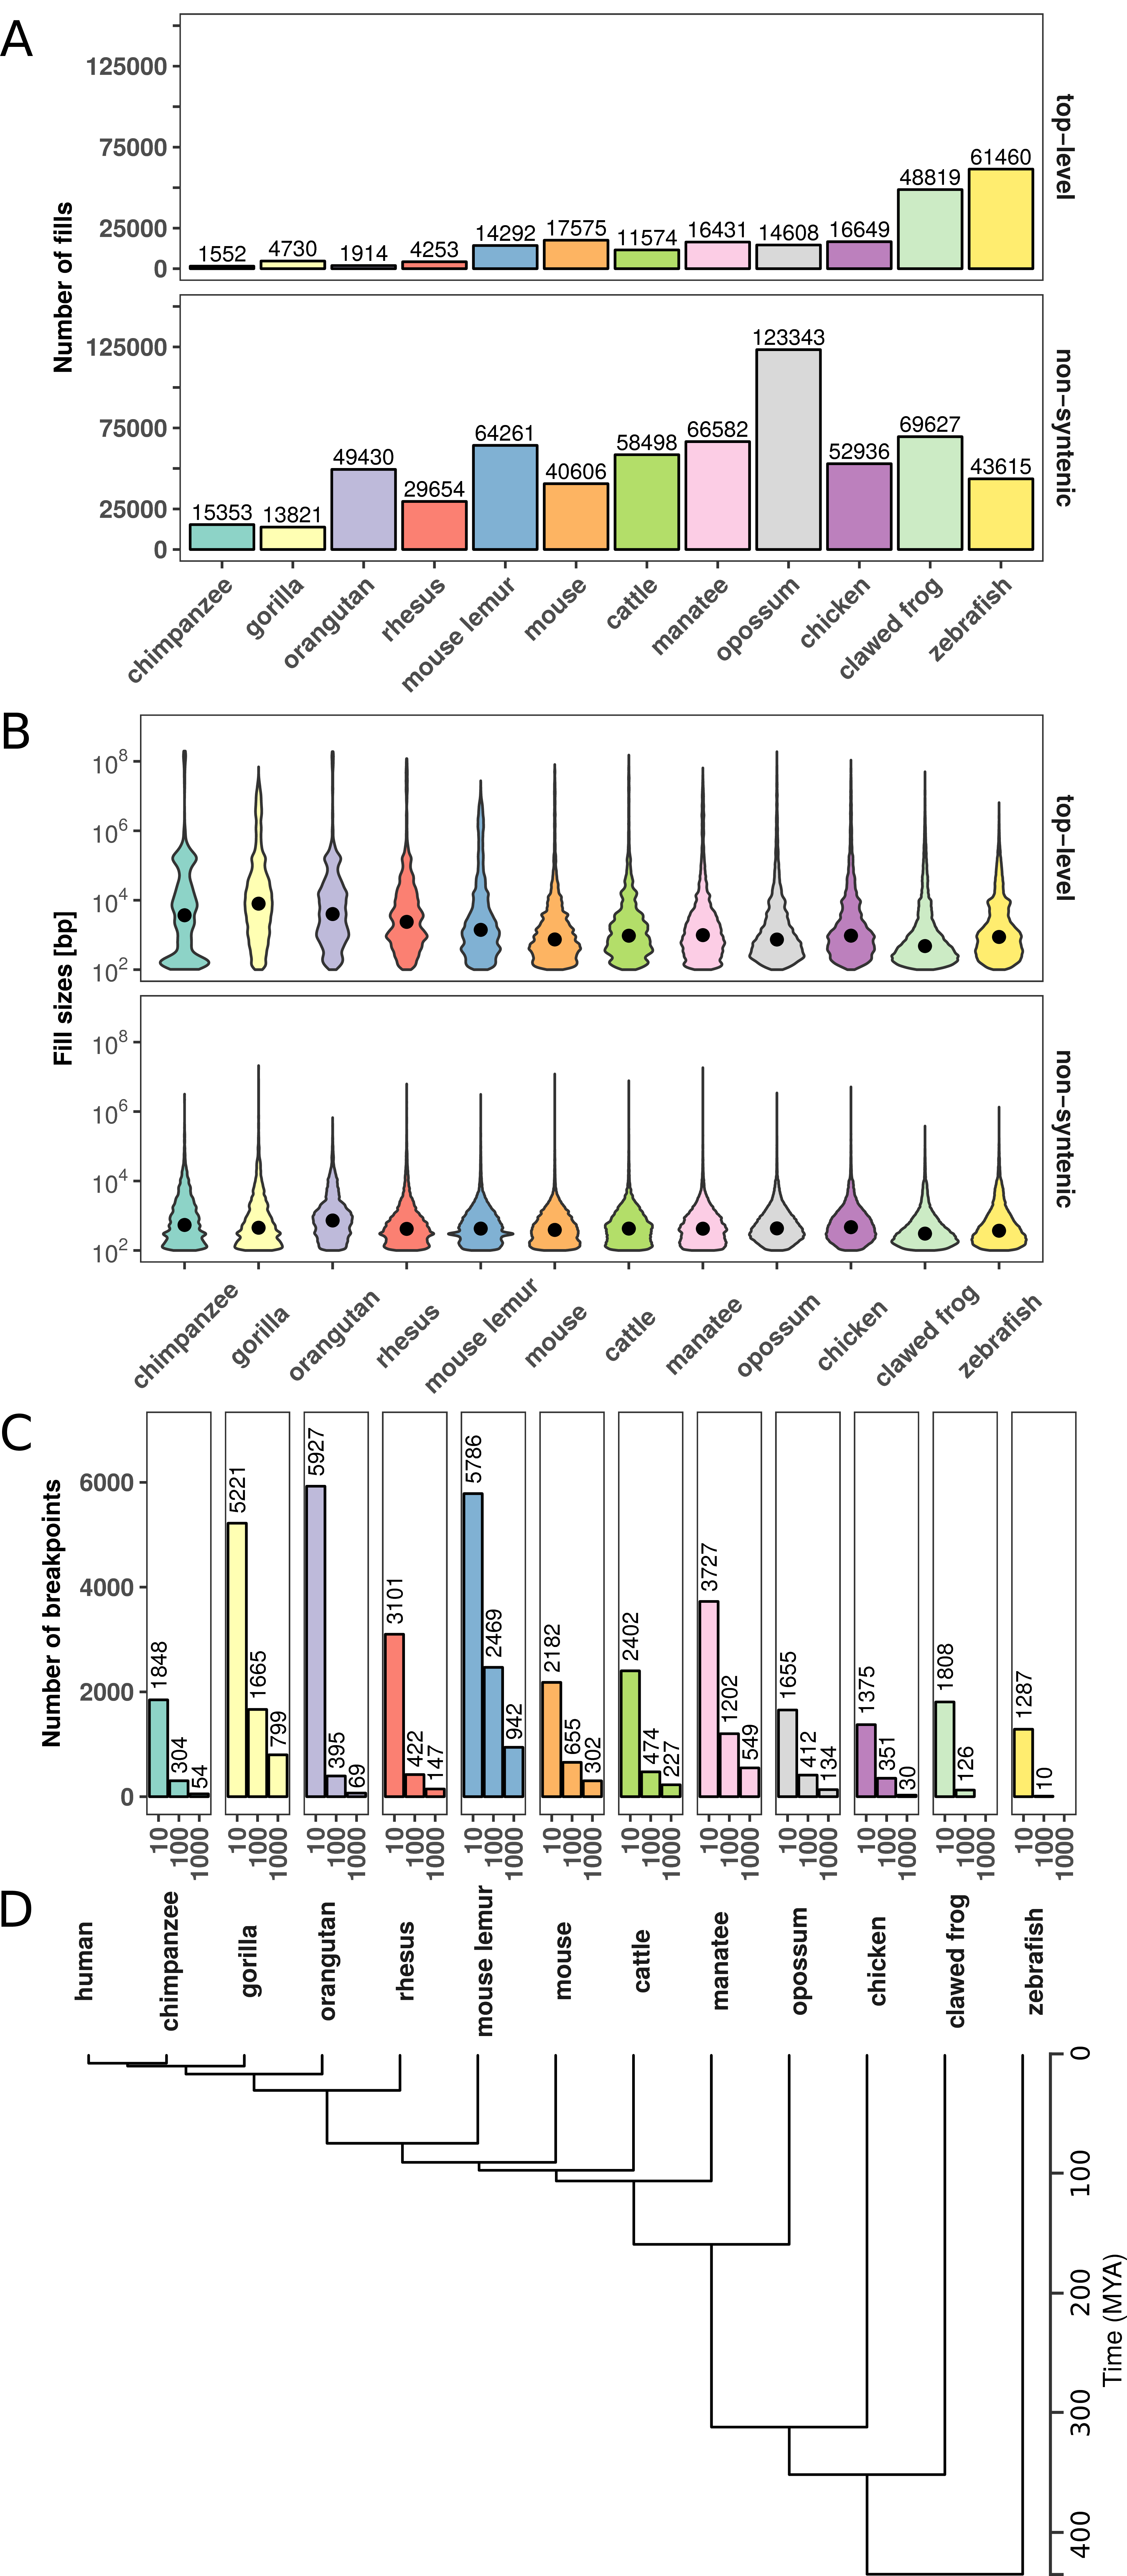
\includegraphics[width=0.5\linewidth]{figures/TAD_evolution/fig1_v02} 

}

\caption{\textbf{Number and size distributions of fill sizes of
whole-genome alignments between human and 12 other species. }
\textbf{(A)} Number of syntenic alignment blocks (fills) between human
(hg38) and 12 other species. Top-level fills are the largest and highest
scoring chains and occur at the top level in the hierarchy in net files
(top panel). Non-syn fills map to different chromosomes as their parent
fills in the net files (bottom panel). \textbf{(B)} Size distribution of
top-level (top panel) and non-syntenic (bottom panel) fills as violin
plot. \textbf{(C)} Number of identified rearrangement breakpoints
between human and 12 other species. Breakpoints are borders of top-level
or non-syn fills that are larger or equal than a given size threshold
(x-axis). \textbf{(D)} Phylogenetic tree with estimated divergence times
according to \href{http://timetree.org/}{\emph{http://timetree.org/}}.}\label{fig:TadEvo1}
\end{figure}















First, we analyzed the number and size distributions of top-level and
non-syntenic fills between human and other species
(Fig~\ref{fig:TadEvo1}). As expected, closely related species such as
chimpanzee and gorilla have in general fewer fills but larger fill sizes
(mean length ≥1 kb), whereas species which are more distant to human,
such as chicken and zebrafish, tend to have more but smaller fills (mean
length ≤ 1 kb, Fig~\ref{fig:TadEvo1}A,B). However, we also observe many
small non-syntenic fills in closely related species, likely arising from
transposon insertions \citep{Mills2006}. As a consequence of the number
of fills and size distributions, we identify different breakpoint
numbers depending on species and size threshold applied. For example,
the whole-genome alignment between human and mouse results in 2182, 655,
and 302 rearrangement breakpoints for size thresholds, 10 kb, 100 kb,
and 1000 kb, respectively (Fig~\ref{fig:TadEvo1}C). Together, the number
and size distributions of syntenic regions reflect the evolutionary
divergence time from human and allow us to identify thousands of
evolutionary rearrangement breakpoints for enrichment analysis at TADs.

\subsection{Rearrangement breakpoints are enriched at TAD
boundaries}\label{rearrangement-breakpoints-are-enriched-at-tad-boundaries}

Next, we analyzed how the identified rearrangement breakpoints are
distributed in the human genome with respect to TADs. We obtained 3,062
TADs identified in human embryonic stem cells (hESC) \citep{Dixon2012}
and 9,274 contact domains from high-resolution \emph{in situ} Hi-C in
human B-lymphoblastoid cells (GM12878) \citep{Rao2014}. To calculate the
number of breakpoints around TADs, we enlarged each TAD region by
+/-50\% of its size and divided the region in 20 equal sized bins. For
each bin we computed the number of overlapping rearrangement
breakpoints. This results in a size-normalized distribution of
rearrangement breakpoints along TAD regions.

\begin{figure}

{\centering 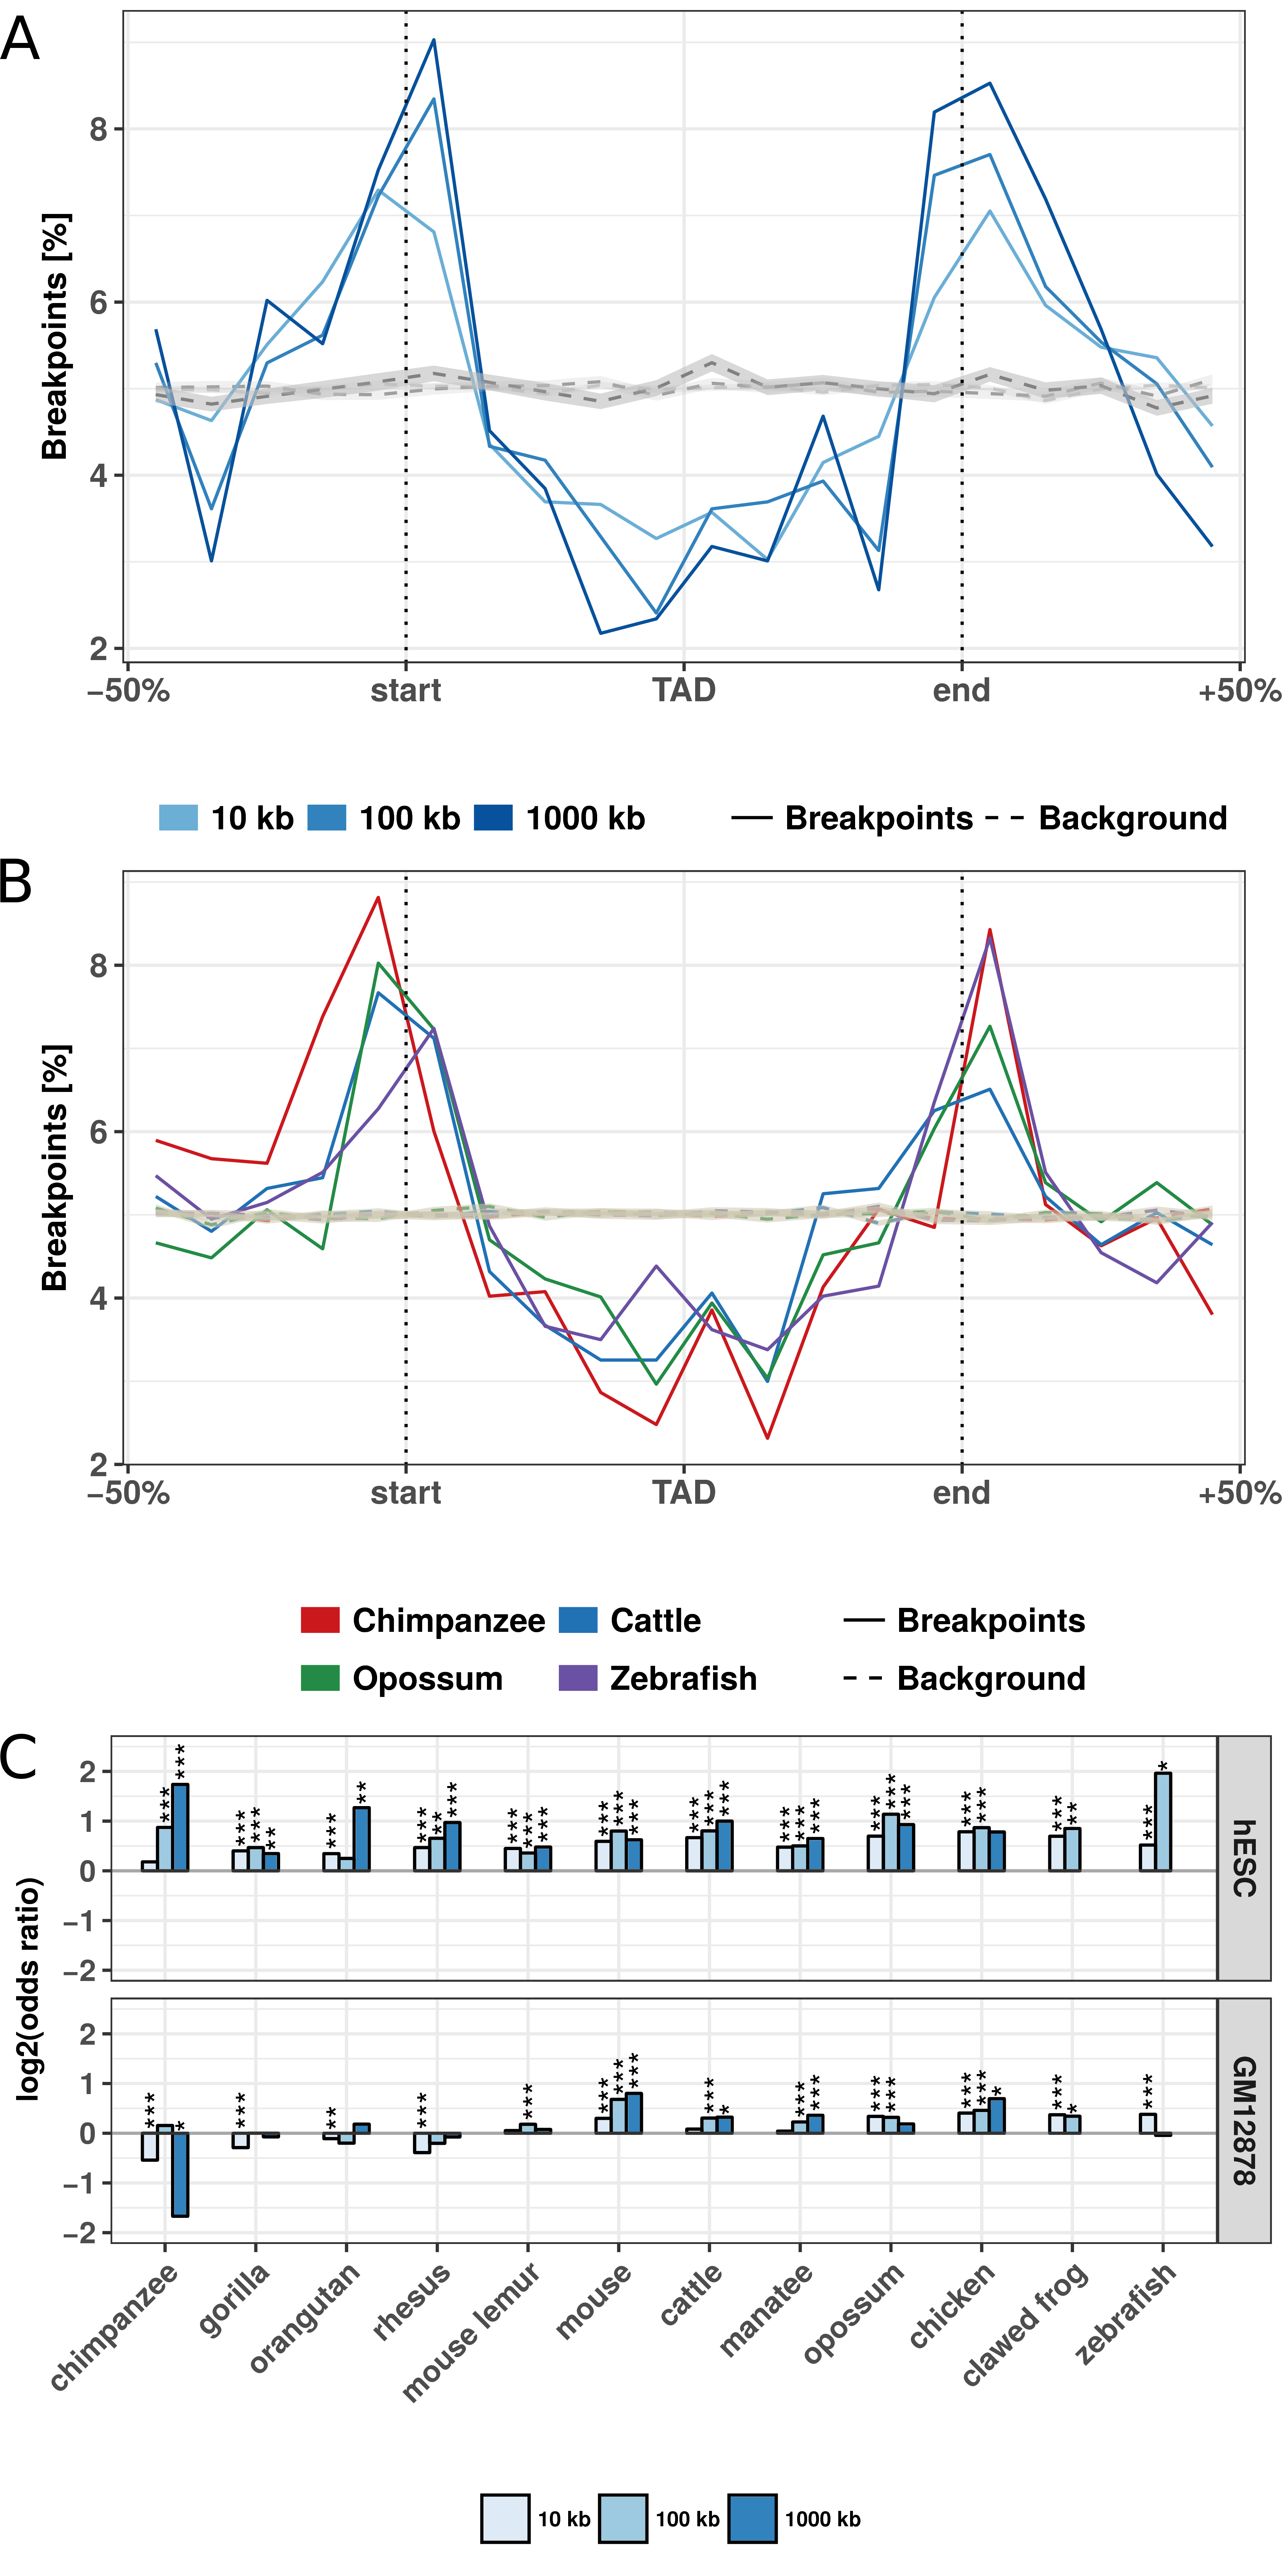
\includegraphics[width=0.5\linewidth]{figures/TAD_evolution/fig2_v02} 

}

\caption{\textbf{Evolutionary rearrangements are enriched at TAD
boundaries.} \textbf{(A)} Distribution of evolutionary rearrangement
breakpoints between human and mouse around hESC TADs. Each TAD and 50\%
of its adjacent sequence was subdivided into 20 bins of equal size, the
breakpoints were assigned to the bins and their number summed up over
the corresponding bins in all TADs. Blue color scale represents
breakpoints from different fill-size thresholds. Dotted lines in gray
show simulated background controls of randomly placed breakpoints.
\textbf{(B)} Distribution of rearrangement breakpoints between human
and: chimpanzee, cattle, opossum, and zebrafish, at 10 kb size threshold
around hESC TADs. Dotted lines in gray show simulated background
controls of randomly placed breakpoints. \textbf{(C)} Enrichment of
breakpoints at TAD boundaries as log-odds-ratio between actual
breakpoints at TAD boundaries and randomly placed breakpoints.
Enrichment is shown for three different fill size thresholds (blue color
scale) and TADs in hESC from \citep{Dixon2012} (top) and contact domains
in human GM12878 cells from \citep{Rao2014} (bottom), respectively.
Asterisks indicate significance of the enrichment using Fisher's exact
test (*p \textless{}= 0.05; **p \textless{}= 0.01; ***p \textless{}=
0.001).}\label{fig:TadEvo2}
\end{figure}






















First, we analyzed the distribution of breakpoints at different size
thresholds between human and mouse at hESC TADs (Fig. 2A). Rearrangement
breakpoints are clearly enriched at TAD boundaries and depleted within
TAD regions. Notably, this enrichment is observed for all size
thresholds applied in the identification of rearrangement breakpoints.
Next, we also analyzed the breakpoints from chimpanzee, cattle, opossum,
and zebrafish (Fig~\ref{fig:TadEvo2}B) at the 10 kb size threshold.
Interestingly, we observed for all species a clear enrichment of
breakpoints at TAD boundaries and depletion within TAD regions. To
quantify this enrichment, we simulated an expected background
distribution of breakpoints by placing each breakpoint 100 times at a
random position of the respective chromosome. We than calculated the
fraction of observed and expected breakpoints that are closer than 40 kb
to a TAD boundary. For all size thresholds and analyzed species, we
computed the log-fold-ratio of actual breakpoints over random
breakpoints at domain boundaries (Fig~\ref{fig:TadEvo2}C). For virtually
all species and size thresholds analyzed, we found breakpoints
significantly enriched at boundaries of TADs and contact domains
(Fig~\ref{fig:TadEvo2}C, \ref{fig:TadEvoS1}). Depletion was only
observed for some combinations of species and size thresholds which have
only very few breakpoints (see Fig~\ref{fig:TadEvo1}C). Furthermore, we
compared the distance of each breakpoint to the closest TAD boundary and
observed nearly always significantly shorter distances for actual
breakpoints compared to random controls (Fig~\ref{fig:TadEvoS2}).
Overall, the enrichment was stronger for TADs in hESC compared to the
contact domains in GM12878. However, these differences were likely due
to different sizes of TADs and contact domains and the nested structure
of contact domains, which overlap each other \citep{Rao2014}.
Rearrangements between human and both closely and distantly related
species are highly enriched at TAD boundaries and depleted within TADs.
These results show (i) that rearrangements are not randomly distributed
in the genome, in agreement with \citep{Farre2015}, and (ii) strong
conservation of TAD regions over large evolutionary time scales,
indicating selective pressure against disruption of TADs, presumably
because of their functional role in gene expression regulation.

\subsection{Clusters of conserved non-coding elements are depleted for
rearrangement
breakpoints}\label{clusters-of-conserved-non-coding-elements-are-depleted-for-rearrangement-breakpoints}

Another interesting feature that can be extracted from whole-genome
alignments are highly conserved non-coding elements (CNEs)
\citep{Polychronopoulos2017}. CNEs are defined as non-protein-coding
sequences of at least 50 bp with over 70\% sequence identity between
distantly related species such as human and chicken
\citep{Polychronopoulos2017}. In the human genome, CNEs cluster around
developmental genes in so-called genomic regulatory blocks (GRBs)
\citep{Kikuta2007}. It has been shown recently that many GRBs coincide
with TADs in human and \emph{Drosophila} genomes \citep{Harmston2017}.
Therefore, we asked whether evolutionary breakpoints are also enriched
at boundaries of GRBs. This would support the idea of a conserved
regulatory environment around important developmental genes. Indeed we
saw a strong enrichment around GRBs (Fig~\ref{fig:TadEvo3}A). This is
consistent with previous studies in \emph{Drosophila} and Fish where CNE
arrays often correspond to syntenic blocks
\citep{Engstrom2007, Dimitrieva2013}.

\begin{figure}

{\centering 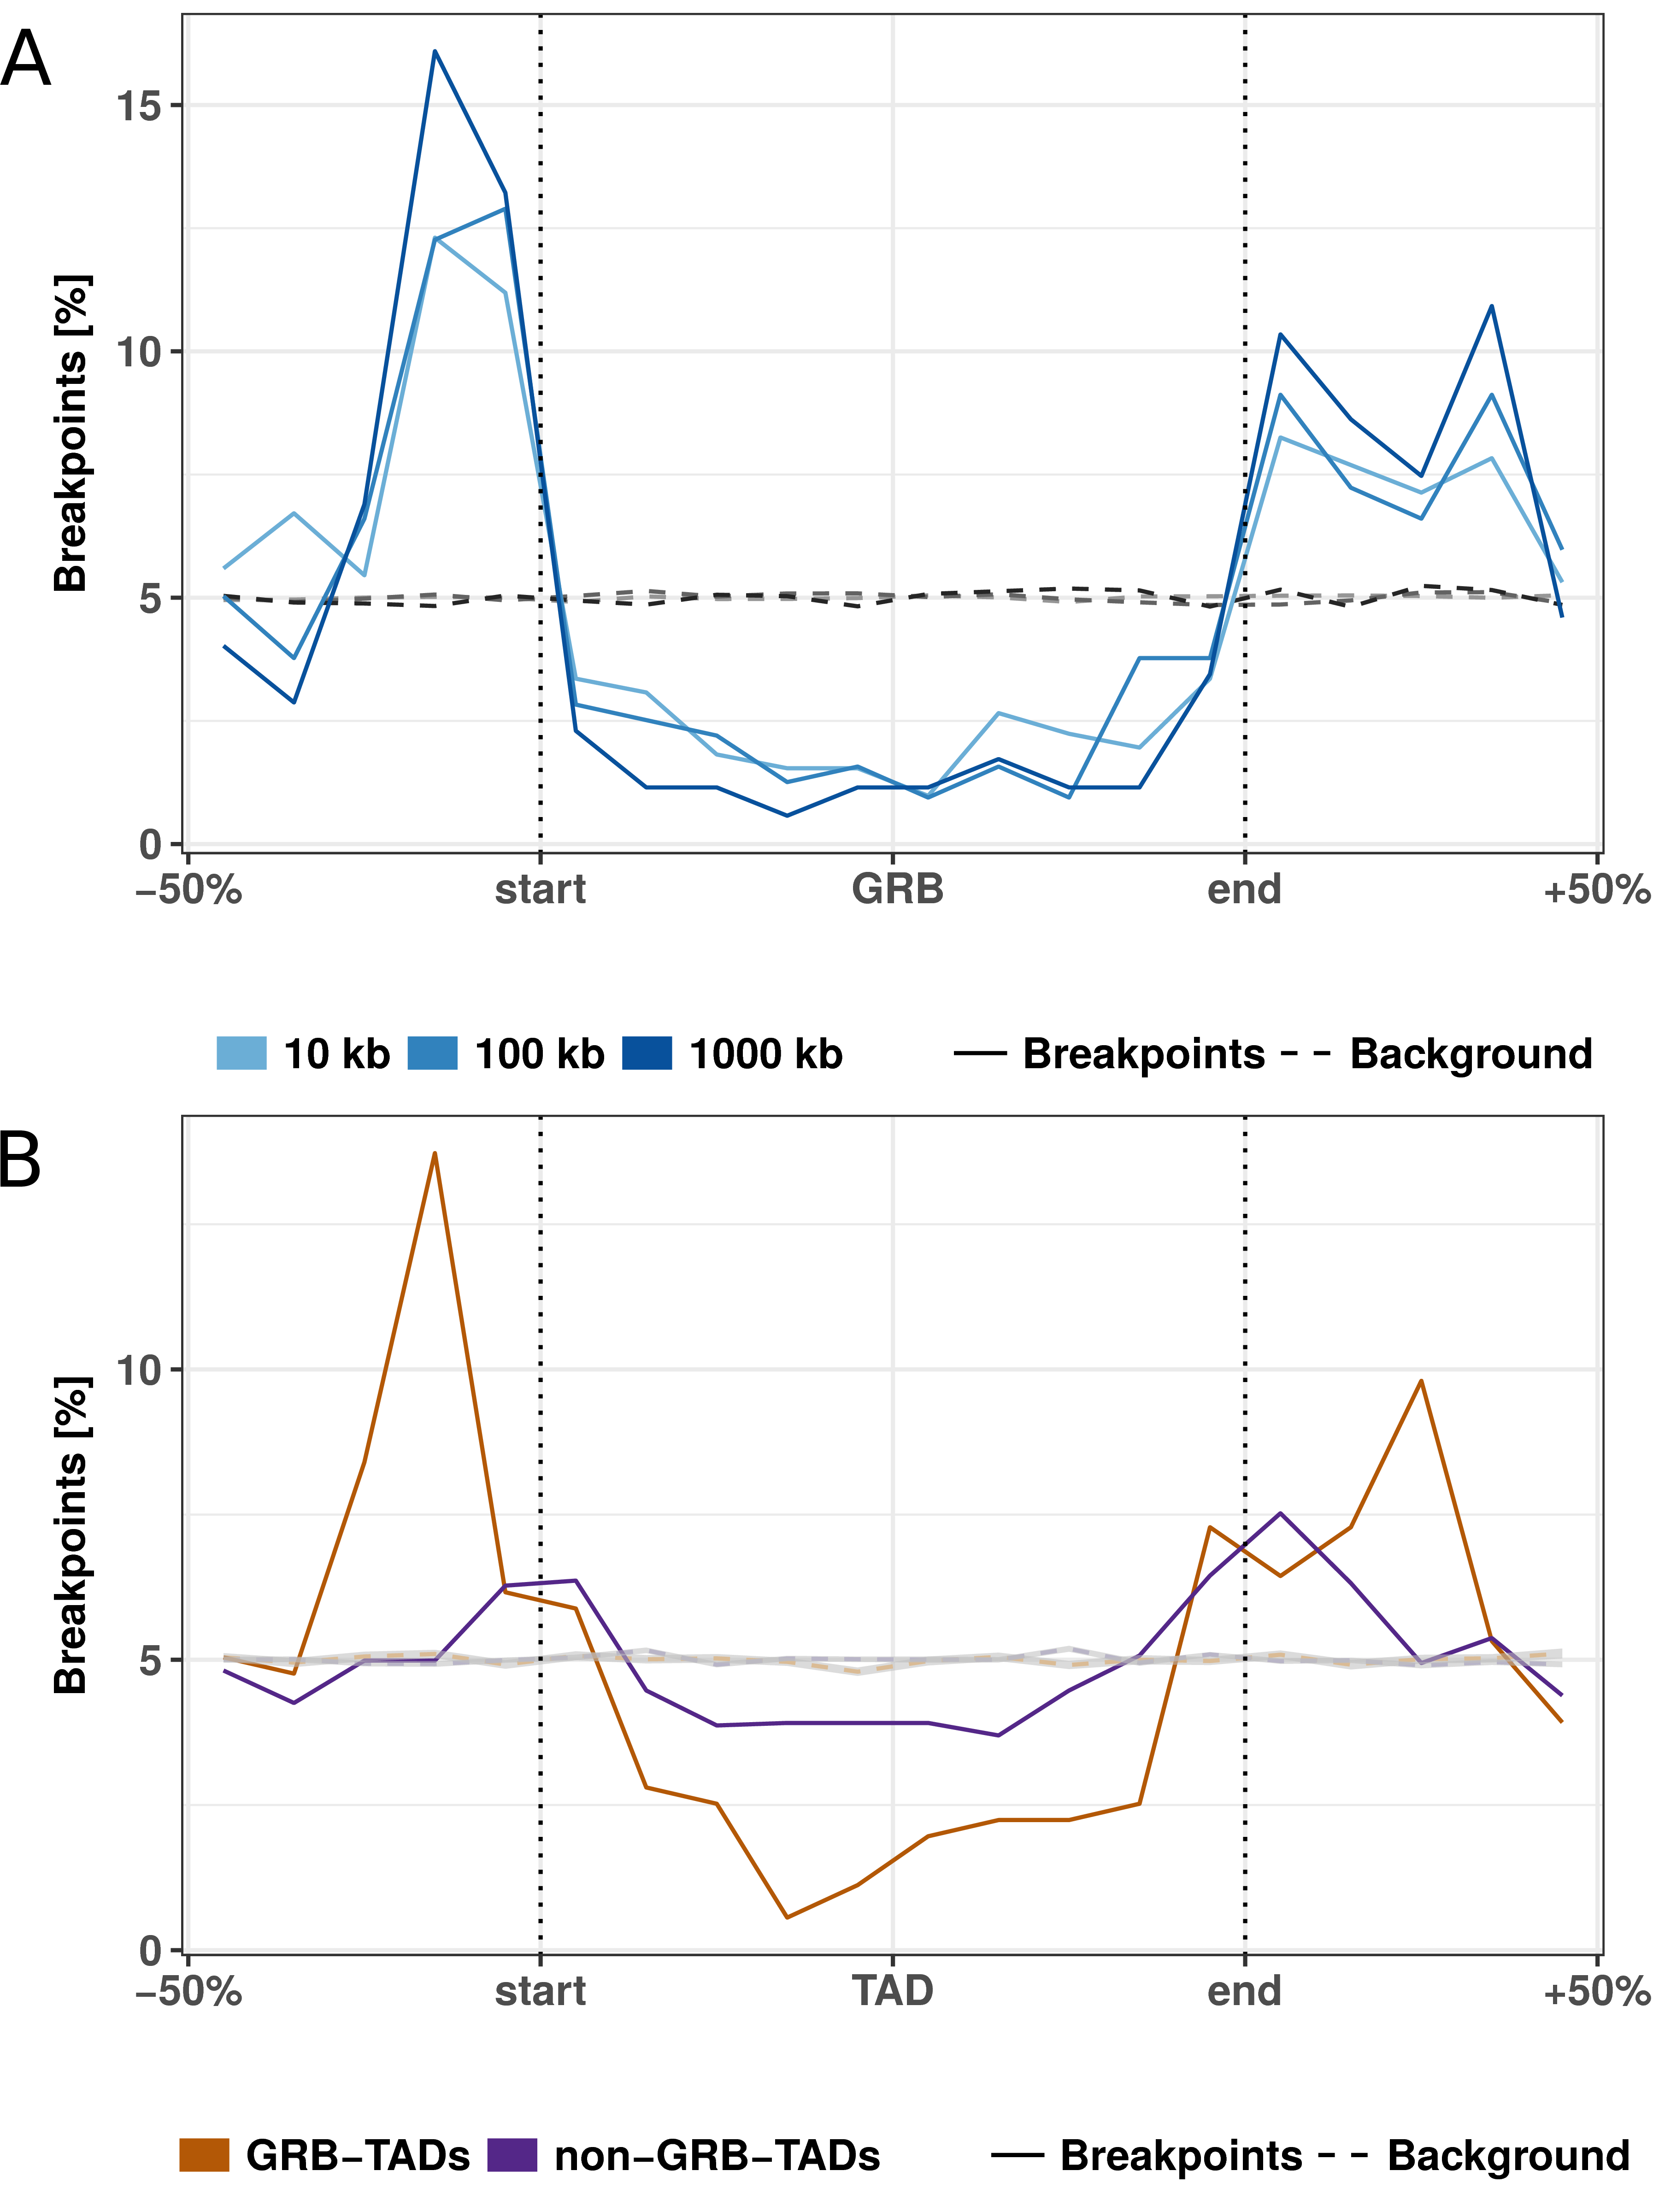
\includegraphics[width=0.5\linewidth]{figures/TAD_evolution/fig3_v02} 

}

\caption{\textbf{Rearrangement breakpoint distribution around GRBs
and GRB-TADs. } \textbf{(A)} Rearrangement breakpoints between mouse and
human around 816 GRBs. \textbf{(B)} Breakpoint distribution around
GRB-TADs and non-GRB-TADs. GRB-TADs are defined as TADs overlapping more
than 80\% with GRBs and non-GRB-TADs have less than 20\% overlap with
GRBs. Breakpoints using a 10 kb fill size threshold are shown.}\label{fig:TadEvo3}
\end{figure}








Next, we subdivided TADs according to their overlap with GRBs in
GRB-TADs (\textgreater{} 80\% overlap) and non-GRB-TADs (\textless{}
20\% overlap) as in the original study \citep{Harmston2017}. As
expected, we observed a higher accumulation of breakpoints at boundaries
and stronger depletion within TADs for GRB-TADs compared to non-GRB-TADs
(Fig~\ref{fig:TadEvo3}B). However, also the non-GRB-TADs, that have less
than 20\% overlap with GRBs, are enriched for rearrangements at TAD
boundaries. This indicates that not only TADs overlapping GRBs are
evolutionary conserved. In summary, we show that human TADs overlapping
clusters of non-coding conserved elements are strongly depleted for
rearrangements, likely due to strong selective pressure on the conserved
regulatory environment around important developmental genes.

\subsection{Rearranged TADs are associated with divergent gene
expression between
species}\label{rearranged-tads-are-associated-with-divergent-gene-expression-between-species}

The enrichment of rearrangement breakpoints at TAD boundaries indicates
that TADs are stable across large evolutionary time scales. However, the
reason for this strong conservation of TAD regions is unclear. A
mechanistic explanation could be that certain chromatin features at TAD
boundaries promote or prevent DNA double strand breaks (DSBs)
\citep{Farre2015, Canela2017}. Alternatively, selective pressure might
act against the disruption of TADs due to their functional importance,
for example in developmental gene regulation
\citep{Nora2013, Farre2015}. TADs constitute a structural framework
determining possible interactions between promoters and cis-regulatory
sequences while prohibiting the influence of other sequences
\citep{Symmons2014, Lupianez2015}. TAD disruption would prevent formerly
established contacts. Rearrangements of TADs might also enable the
recruitment of new cis-regulatory sequences which would alter the
expression patterns of genes in rearranged TADs
\citep{Lupianez2015, Redin2016}. Because of these detrimental effects,
rearranged TADs should largely be eliminated by purifying selection.
However, rearrangement of TADs could also enable the expression of genes
in a new context and be selected if conferring an advantage. Therefore,
we hypothesized that genes within conserved TADs might have a more
stable gene expression pattern across tissues, whereas genes in
rearranged TADs between two species might have a more divergent
expression between species.

To test this, we analyzed the conservation of gene expression of
ortholog genes between human and mouse across 19 matched tissues from
the FANTOM5 project (\protect\hyperlink{TadEvoSupTab}{Table S1})
\citep{Forrest2014}. If a human gene and its mouse ortholog have high
correlation across matching tissues, they are likely to have the same
regulation and eventually similar functions. Conversely, low correlation
of expression across tissues can indicate functional divergence during
evolution, potentially due to altered gene regulation.

First, we separated human genes according to their location within TADs
or outside of TADs. From 12,696 human genes with expression data and a
unique one-to-one ortholog in mouse
(\protect\hyperlink{TadEvoSupTab}{Table S2}), 1,525 have a transcription
start site (TSS) located outside hESC TADs and 11,171 within. Next, we
computed for each gene its expression correlation with mouse orthologs
across 19 matching tissues. Genes within TADs have significantly higher
expression correlation with their mouse ortholog (median R = 0,340)
compared to genes outside TADs (mean R = 0,308, p = 0.0015,
Fig~\ref{fig:TadEvo4}A). This indicates higher conservation of gene
regulation in TADs and is consistent with the observation of
housekeeping genes at TAD boundaries \citep{Dixon2012} and the role of
TADs in providing conserved regulatory environments for gene regulation
\citep{Harmston2017, Ibn-Salem2017}.

\begin{figure}

{\centering 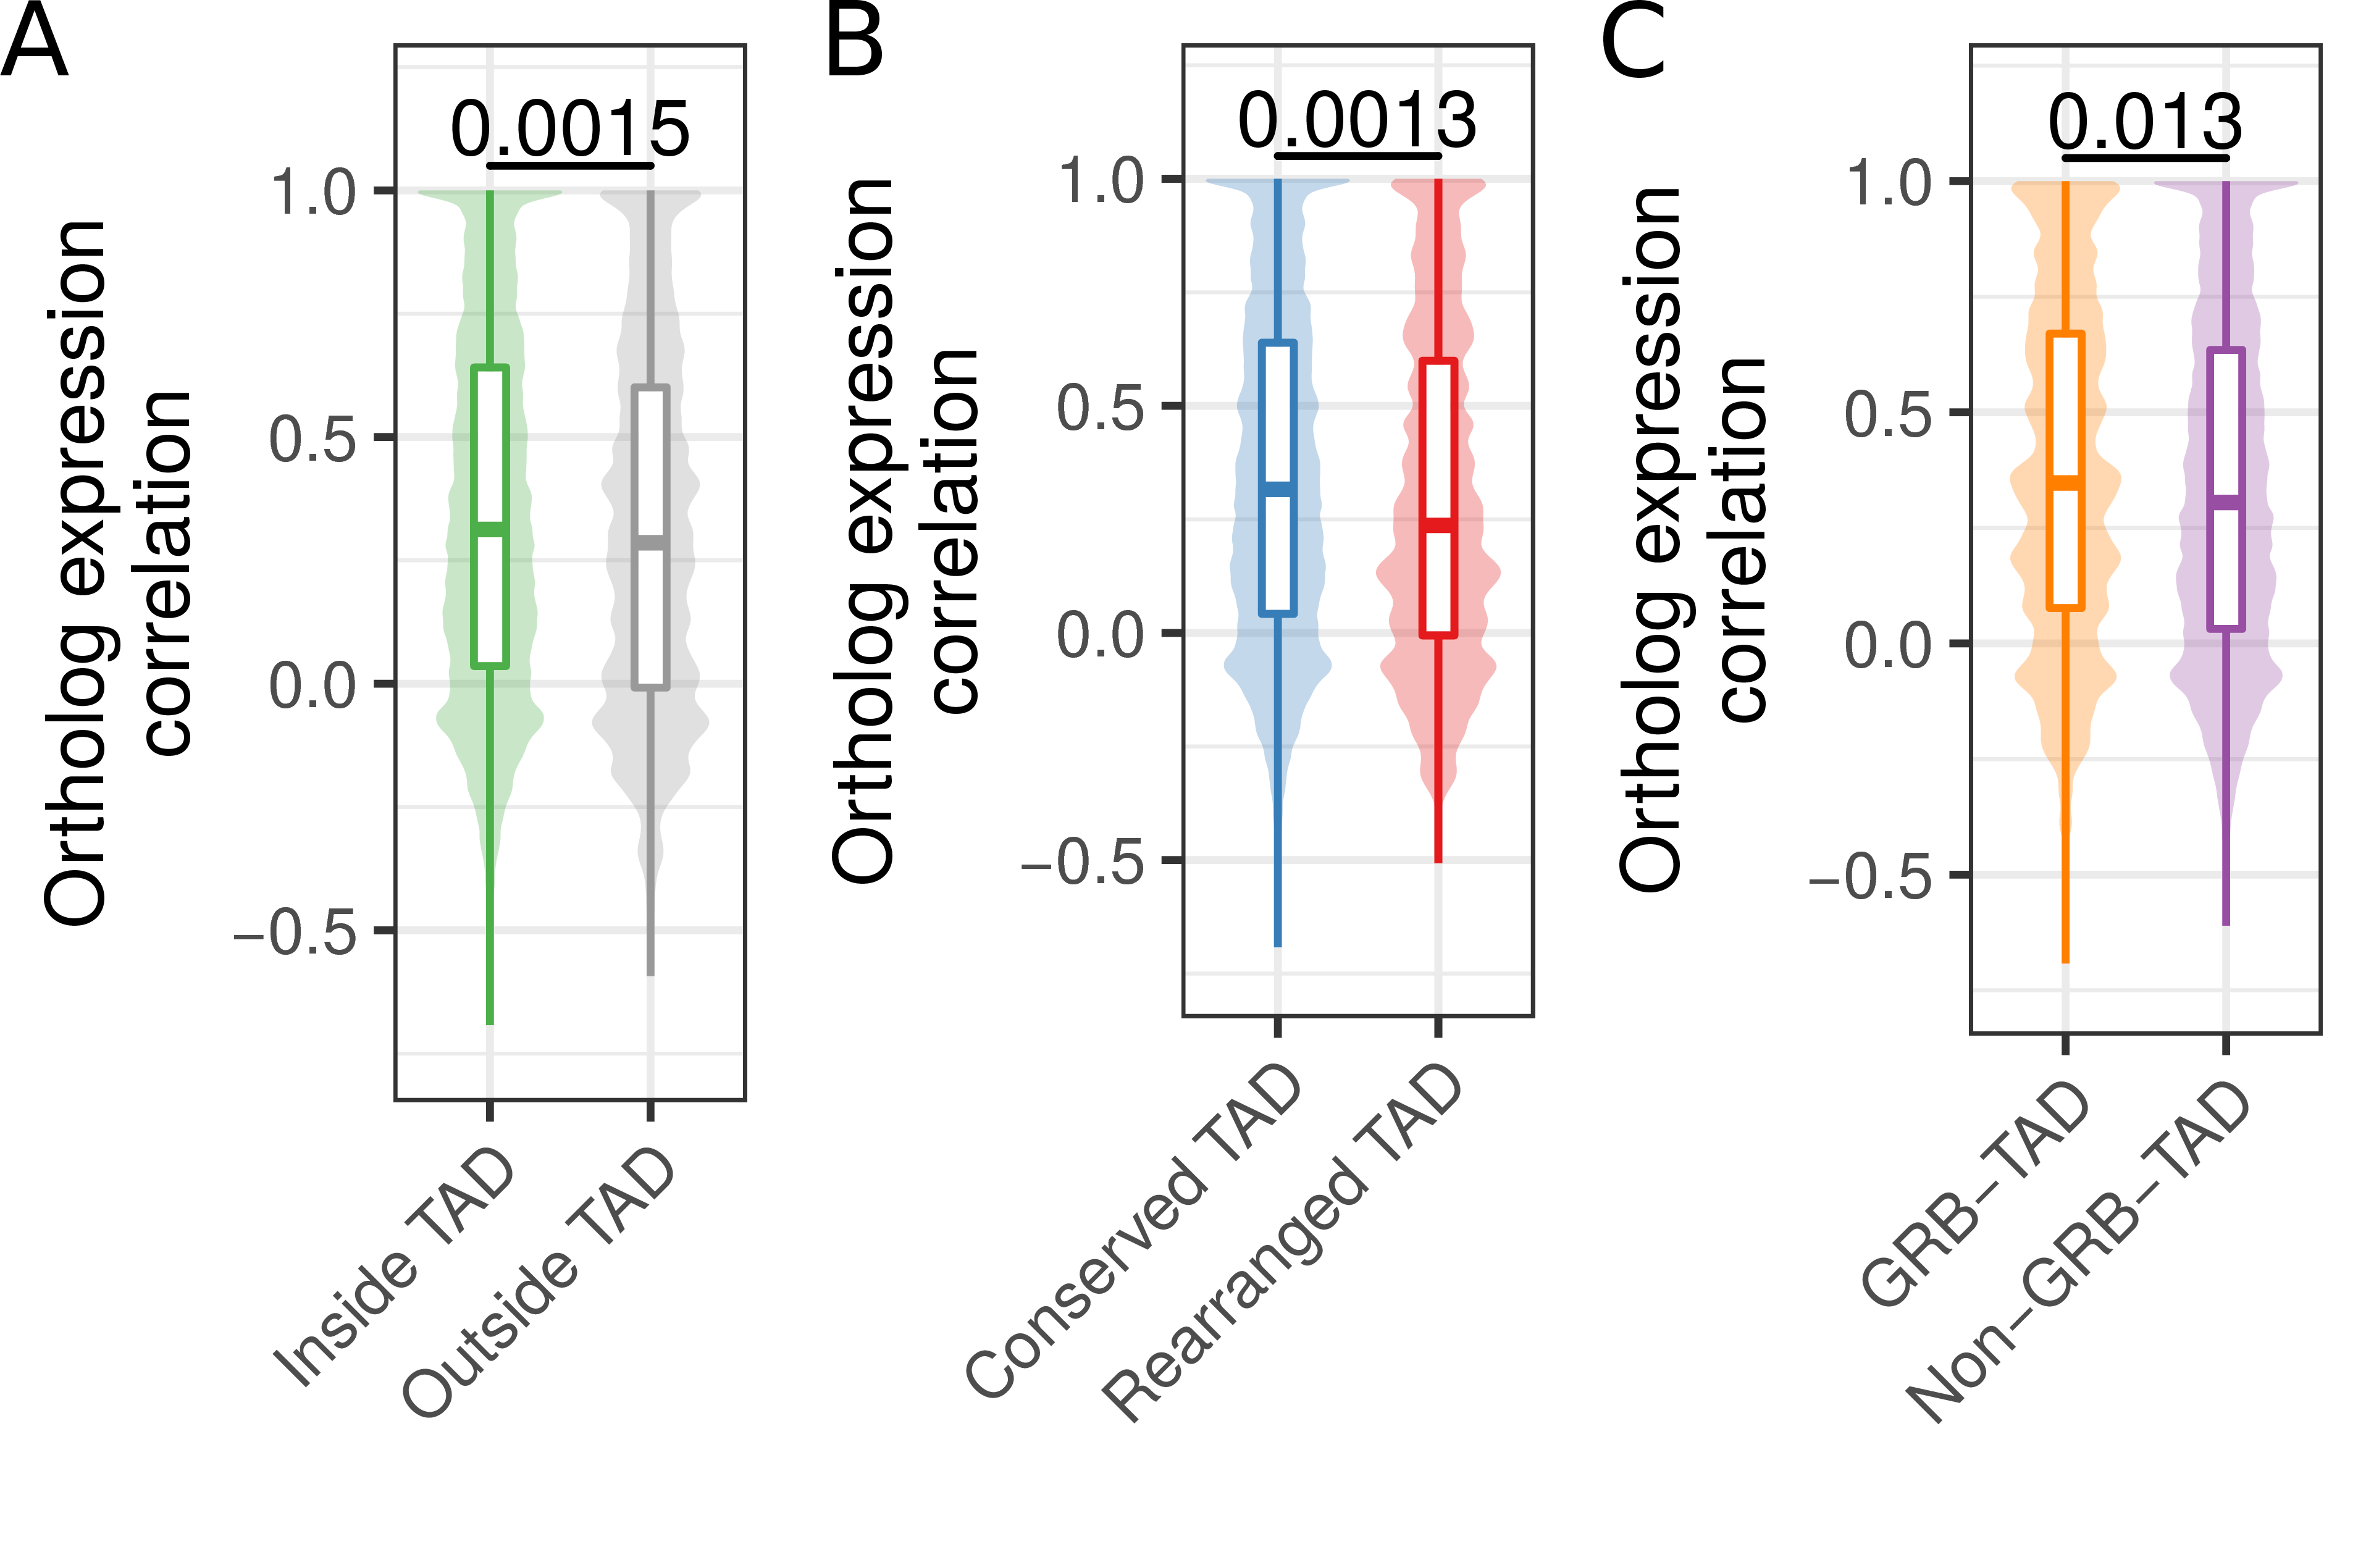
\includegraphics[width=0.8\linewidth]{figures/TAD_evolution/fig4_v04} 

}

\caption{\textbf{Ortholog gene expression correlation across
tissues in conserved and rearranged TADs.} \textbf{(A)} Expression
correlation of orthologs across 19 matching tissues in human and mouse
for human genes within or outside of hESC TADs. \textbf{(B)} Expression
correlation of orthologs across 19 matching tissues in human and mouse
for genes in conserved or rearranged TADs. \textbf{(C)} Expression
correlation of orthologs across 19 matching tissues in human and mouse
for genes in GRB-TADs and non-GRB TADs. All P-values according to
Wilcoxon rank-sum test.}\label{fig:TadEvo4}
\end{figure}











Next, we further subdivided TADs in two groups, rearranged and
conserved, according to syntenic blocks and rearrangements between human
and mouse genomes. In brief, a TAD is defined as conserved, if it is
completely enclosed by a syntenic alignment block and does not overlap
any rearrangement breakpoint. Conversely, a rearranged TAD is not
enclosed by a syntenic alignment block and overlaps at least one
breakpoint that is farther than 80 kb from its boundary (see Methods).
For the hESC TAD data set, this leads to 2,542 conserved and 137
rearranged TADs. The low number of rearranged TADs is consistent with
the depletion of rearrangement breakpoints within TADs in general (Fig.
2). In total 8,740 genes in conserved and 645 genes in rearranged TADs
could be assigned to a one-to-one ortholog in mouse and are contained in
the expression data set. The expression correlation with mouse orthologs
were significantly higher for genes in conserved TADs (median R = 0.316)
compared to genes in rearranged TADs (median R = 0.237, p = 0.0013)
(Fig~\ref{fig:TadEvo4}B). This shows that disruptions of TADs by
evolutionary rearrangements are associated with less conserved gene
expression profiles across tissues. Although not significant, we also
observed a slightly higher expression correlation for 1,003 genes in
GRB-TADs compared to 8,038 genes in non-GRB TADs
(Fig~\ref{fig:TadEvo4}C, p = 0.13).

In summary, we observed higher expression correlation between
orthologs\\
for human genes inside TADs than outside. Moreover, we saw that genes in
rearranged TADs show lower gene expression conservation than those in
conserved TADs. These results not only support a functional role of TADs
in gene regulation, but further support the hypothesis that TAD regions
are subjected to purifying selection against their disruption by
structural variations such as rearrangements.

\section{Discussion}\label{discussion-1}

Our analysis of rearrangements between human and 12 diverse species
shows that TADs are largely stable units of genomes, which are often
reshuffled as a whole instead of disrupted by rearrangements.
Furthermore, the decreased expression correlation with orthologs in
mouse and human in rearranged TADs shows that disruptions of TADs are
associated with changes in gene regulation over large evolutionary time
scales.

TADs exert their influence on gene expression regulation by determining
the set of possible interactions of cis-regulatory sequences with their
target promoters \citep{Nora2012, Symmons2014, Schoenfelder2015}. This
might facilitate the cooperation of several sequences that is often
needed for the complex spatiotemporal regulation of transcription
\citep{Andrey2017}. The disruption of these enclosed regulatory
environments enables the recruitment of other cis-regulatory sequences
and might prevent formerly established interactions
\citep{Montavon2012}. The detrimental effects of such events have been
shown in the study of diseases \citep{Redin2016, Zepeda-Mendoza2017}.
There are also incidences where pathogenic phenotypes could be
specifically attributed to enhancers establishing contacts to promoters
that were formerly out of reach because of intervening TAD boundaries
\citep{Ibn-Salem2014, Lupianez2015, Spielmann2012}. This would explain
the selective pressure to maintain TAD integrity over large evolutionary
distances and why we observe higher gene expression conservation for
human genes within TADs compared to genes outside TADs.

Disruptions of TADs by large-scale rearrangements change expression
patterns of orthologs across tissues and these changes might be
explained by the altered regulatory environment which genes are exposed
to after rearrangement \citep{Farre2015}.

Our results are largely consistent with the reported finding that many
TADs correspond to clusters of conserved non-coding elements (GRBs)
\citep{Harmston2017}. We observe a strong depletion of evolutionary
rearrangements in GRBs and enrichment at GRB boundaries. This is
consistent with comparative genome analysis revealing that GRBs largely
overlap with micro-syntenic blocks in \emph{Drosophila}
\citep{Engstrom2007} and fish genomes \citep{Dimitrieva2013}. However,
over 60\% of human hESC TADs do not overlap GRBs \citep{Harmston2017},
raising the question of whether only a small subset of TADs are
conserved. Interestingly, we find also depletion of rearrangements in
non-GRB-TADs. This indicates that our rearrangement analysis identifies
conservation also for TADs that are not enriched for CNEs. High
expression correlation of orthologs in conserved TADs suggestss that the
maintenance of expression regulation is important for most genes and
probably even more crucial for developmental genes which are frequently
found in GRBs.

Previous work using comparative Hi-C analysis in four mammals revealed
that insulation of TAD boundaries is robustly conserved at syntenic
regions, illustrating this with a few examples of rearrangements between
mouse and dog genomes, which were located in both species at TAD
boundaries \citep{VietriRudan2015}. The results of our analysis of
thousands of rearrangements between human and 12 other species confirmed
and expanded these earlier observations.

The reliable identification of evolutionary genomic rearrangements is
difficult. Especially for non-coding genomic features like TAD
boundaries, it is important to use approaches that are unbiased towards
coding sequence. Previous studies identified rearrangements by
interrupted adjacency of ortholog genes between two organisms
\citep{VietriRudan2015, Pevzner2003}. However, such an approach assumes
equal inter-genic distances, which is violated at TAD boundaries, which
have in general higher gene density \citep{Dixon2012, Hou2012}. To avoid
this bias we used whole-genome-alignments. However, low quality of the
genome assembly of some species might introduce alignment problems and
potentially false positive rearrangement breakpoints.

Rearrangements are created by DNA double strand breaks (DSBs), which are
not uniquely distributed in the genome. Certain genomic features, such
as open chromatin, active transcription and certain histone marks are
shown to be enriched at DSBs in somatic translocation sites
\citep{Roukos2014} and evolutionary rearrangements
\citep{Murphy2005, Hinsch2006}. Furthermore, induced DSBs and somatic
translocation breakpoints are enriched at chromatin loop anchors
\citep{Canela2017}. This opens the question of whether our finding of
significantly enriched evolutionary rearrangement breakpoints at TAD
boundaries could be explained by the molecular properties of the
chromatin at TAD boundaries, rather than by the selective pressure to
keep TAD function. Although, we cannot distinguish the two explanations
entirely, our gene expression analysis indicates stronger conservation
of gene expression in conserved TADs and more divergent expression
patterns in rearranged TADs. This supports a model in which disruption
of TADs are most often disadvantageous for an organism. Structural
variations disrupting TADs can lead to miss regulation of neighboring
genes as shown for genetic diseases
\citep{Ibn-Salem2014, Lupianez2015, Redin2016, Franke2016} and cancers
\citep{Hnisz2016, Northcott2014, Weischenfeldt2016}.

Interestingly, we observed higher gene expression conservation for human
genes within TADs compared to genes outside TADs. The larger syntenic
structure of TADs might conserve the regulation likely by maintaining
the proximity of promoters and cis-regulatory sequences while genes
outside such frameworks are more exposed to changing genomic landscapes,
presumably resulting in a greater susceptibility to the recruitment of
regulatory sequences.

Apart from the described detrimental effects, our results suggest that
TAD rearrangements occurred between genomes of human and mouse and led
to changes in expression patterns of many orthologous genes. Since this
is likely attributed to changing regulatory environments, it is also
conceivable that some rearrangements led to a gain of function. Hence,
TAD rearrangements might also provide a vehicle for evolutionary
innovation. A single TAD reorganization has the potential to affect the
regulation of a whole set of genes in contrast to the more confined
consequences of other types of mutations \citep{Acemel2017}. Since it is
also believed that changes in cis-regulatory sequences of developmental
genes play a big part in evolutionary innovation \citep{Carroll2008},
the development of the enormous diversity of animal traits in evolution
might have been promoted by the rearrangement of structural domains.
This is consistent with a model in which new genes can arise by
tandem-duplication and during evolution are then re-located to other
environments \citep{Ibn-Salem2017}. These changes might have facilitated
significant leaps in morphological evolution explaining the emergence of
features that could not appear in small gradual steps. Following this
hypothesis, TADs would not only constitute structural entities that
perform the function of maintaining an enclosed regulatory landscape but
could also be a driving force for change by exposing many genes at once
to different genomic environments following single events of genomic
rearrangement.

\section{Conclusion}\label{conclusion-1}

Our results indicate that TADs represent conserved functional building
blocks of the genome. We have shown that the majority of evolutionary
rearrangements do not affect the integrity of TADs and instead
breakpoints are strongly clustered at TAD boundaries. This leads to the
conclusion that TADs constitute conserved building blocks of the genome
that are often reshuffled as a whole rather than disrupted during
evolution. The conservation of TAD regions can be explained by
detrimental effects of disrupting cis-regulatory environments that are
essential for the spatio-temporal control of gene expression. Indeed we
observe a significant association of conserved gene expression in intact
TADs and divergent expression patterns in rearranged TADs explaining
both why there could be selective pressure on the integrity of TADs over
large evolutionary time scales, but also how TAD rearrangement can
explain evolutionary leaps.

\section{Methods}\label{methods}

\subsection{Rearrangement breakpoints from whole-genome
alignments}\label{rearrangement-breakpoints-from-whole-genome-alignments}

Rearrangement breakpoints were identified between human and 12 selected
vertebrate species from whole-genome-alignment data (Table 1). Alignment
data were downloaded as net files from UCSC Genome Browser for human
genome hg38 and the genomes listed in Table 1. The whole-genome data
consists of consecutive alignment blocks that are chained and
hierarchically ordered in the so-called nets \citep{Kent2003}. Chains
represent blocks of interrupted syntenic regions and may include larger
gaps. When hierarchically arranged in a net file, child chains can
complement their parents when they align nearby segments that fill the
alignment gaps of their parents but may also break the synteny when
incorporating distal segments. We implemented a computer program to
extract rearrangement breakpoints from net files based on the length and
type of fills. Start and end points of top-level or non-syntenic fills
are reported as rearrangement breakpoint if the fill exceeds a given
size threshold. We used different size thresholds to optimize both the
number of identified breakpoints and to avoid biases of transposable
elements that might be responsible for many small interruptions of
alignment chains. In this way, we extracted rearrangement breakpoints
between human and 12 genomes using size thresholds of 10 kb, 100 kb, and
1000 kb. To compare breakpoints to TADs we converted the breakpoint
coordinates from hg38 to hg19 genome assembly using the liftOver tool
from UCSC Genome Browser \citep{Hinrichs2006}.

\subsection{Topologically associating domains and contact
domains}\label{topologically-associating-domains-and-contact-domains}

We obtained topologically associating domain (TAD) calls from published
Hi-C experiments in human embryonic stem cells (hESC) \citep{Dixon2012}
and contact domains from published \emph{in situ} Hi-C experiments in
human GM12878 cells \citep{Rao2014}. Genomic coordinates of hESC TADs
were converted from hg18 to hg19 genome assembly using the UCSC liftOver
tool \citep{Hinrichs2006}.

\subsection{Breakpoint distributions at
TADs}\label{breakpoint-distributions-at-tads}

To quantify the number of breakpoints around TADs and TAD boundaries we
enlarged TAD regions by 50\% of their total length on each side. The
range was then subdivided into 20 equal sized bins and the number of
overlapping breakpoints computed. This results in a matrix in which rows
represent individual TADs and columns represent bins along TAD regions.
The sum of each column indicates the number of breakpoints for
corresponding bins and therefore the same relative location around TADs.
For comparable visualization between different data sets, the
column-wise summed breakpoint counts were further normalized as percent
values of the total breakpoint number in the matrix.

\subsection{Quantification of breakpoint
enrichment}\label{quantification-of-breakpoint-enrichment}

To quantify the enrichment of breakpoints at domain boundaries, we
generated random breakpoints as background control. For each chromosome,
we placed the same number of actual breakpoints at a random position of
the chromosome. For each breakpoint data set we simulated 100 times the
same number of random breakpoints. We then computed the distribution of
random breakpoints around TADs in the same way as described above for
actual breakpoints. To compute enrichment of actual breakpoints compared
to simulated controls, we classified each breakpoint located in a window
of 400 kb around TAD borders in either close to a TAD boundary, if
distance between breakpoint and TAD boundary was smaller or equal to 40
kb or as distant, when distance was larger than 40 kb. This results in a
contingency table of actual and random breakpoints that are either close
or distal to TAD boundaries. We computed log odds ratios as effect size
of enrichment and p-values according to Fishers two-sided exact test.
Additionally, we compared the distance of all actual and random
breakpoints to their nearest TAD boundary using the Wilcoxon's rank-sum
test.

\subsection{Expression data for mouse and human
orthologs}\label{expression-data-for-mouse-and-human-orthologs}

Promoter based expression data from CAGE analysis in human and mouse
tissues from the FANTOM5 project \citep{Forrest2014} were retrieved from
the EBI Expression Atlas \citep{Hinrichs2006} as baseline expression
values per gene and tissue. The meta data of samples contains tissue
annotations as term IDs from Uberon, an integrated cross-species
ontology covering anatomical structures in animals \citep{Herrero2016}.
Human and mouse samples were assigned to each other if they had the same
developmental stage and matching Uberon term IDs. This resulted in 19
samples for each organism with corresponding tissues.

We used the R package biomaRt to retrieve all human genes in the Ensembl
database (version grch37.ensembl.org) and could assign 13,065 to
ortholog genes in mouse by allowing only the one-to-one orthology type
\citep{Herrero2016}. Of these ortholog pairs, 12,696 are contained in
the expression data described above. For each pair of orthologs we
computed the correlation of expression values across matching tissues as
Pearson's correlation coefficient.

\subsection{Classification of TADs and genes according to rearrangements
and
GRBs}\label{classification-of-tads-and-genes-according-to-rearrangements-and-grbs}

We classified hESC TADs according to rearrangements between human and
mouse genomes. We define a TAD as conserved if it is completely enclosed
within a fill in the net file and no rearrangement breakpoint from any
size threshold is located in the TAD region with a distance larger than
80 kb from the TAD boundary. A TAD is defined as rearranged, if the TAD
is not enclosed completely by any fill in the net file, overlaps at
least one breakpoint inferred using a 1000 kb fill size threshold, and
this breakpoint is further than 80 kb away from each TAD boundary. TADs
were also classified according to their overlap with GRBs as in
\citep{Harmston2017}. A given TAD is a GRB-TAD if it overlaps with more
than 80\% of the TAD size with a GRB. A TAD is classified as non-GRB if
it has less than 20\% overlap with GRBs. The 12,696 human genes with
mouse ortholog and expression data were grouped according to their
location with respect to hESC TADs. We used the transcription start site
(TSS) of the longest transcript per gene to group each gene as within
TAD if the TSS overlaps a hESC TAD or as outside TADs, if not.
Furthermore, we grouped genes in TADs according to conserved or
rearranged TADs and separately according to GRB and non-GRB TADs.

\subsection{Source code and implementation
details}\label{source-code-and-implementation-details}

The source code of the entire analysis described here is available on
GitHub:
\href{https://github.com/Juppen/TAD-Evolution}{\emph{https://github.com/Juppen/TAD-Evolution}}.
The identification of breakpoints and extraction of fills from
whole-genome alignment data was implemented in Python scripts. Reading
of BED files and overlap calculations with TADs and TAD bins were
computed in R with Bioconductor \citep{Huber2015} packages rtracklayer
\citep{Lawrence2009} and GenomicRanges \citep{Lawrence2013}. Gene
coordinates and ortholog assignments were retrieved from Ensemble data
base (version grch37.ensembl.org) using the package biomaRt
\citep{Durinck2009}. For data integration and visualization we used R
packages from tidyverse \citep{Wickham2017}.

\section{Declarations}\label{declarations}

\subsection{Ethics approval and consent to
participate}\label{ethics-approval-and-consent-to-participate}

Not applicable

\subsection{Consent for publication}\label{consent-for-publication}

Not applicable

\subsection{Availability of data and
material}\label{availability-of-data-and-material}

The source code of all analysis is available on GitHub:
\href{https://github.com/Juppen/TAD-Evolution}{\emph{https://github.com/Juppen/TAD-Evolution}}.
All the genomic data used for analyses are freely available to be
downloaded from the UCSC Genome Browser and EBI Expression Atlas with
identifiers listed in Table 1 and \protect\hyperlink{TadEvoSupTab}{Table
S1}.

\subsection{Competing interests}\label{competing-interests}

The authors declare that they have no competing interests.

\subsection{Funding}\label{funding}

Not applicable.

\subsection{Authors` contributions}\label{authors-contributions}

JK and JI developed and implemented the methods and performed the
analysis. JI conceived the study. JK wrote the first draft of the
manuscript. JK, MA and JI wrote the manuscript. MA supervised the study.

\subsection{Acknowledgments}\label{acknowledgments}

The authors thank all members of the CBDM group for fruitful
discussions.

\section{Tables}\label{tables}

\subsection{Table 1}\label{table-1}

\begin{verbatim}
    Species used for breakpoint identification from whole-genome
    alignments with human.
\end{verbatim}

\begin{longtable}[]{@{}llll@{}}
\toprule
Common name & Species & Genome Assembly & Divergence to human
(mya)\tabularnewline
Chimpanzee & \emph{Pan troglodytes} & panTro5 & 6.65\tabularnewline
Gorilla & \emph{Gorilla gorilla gorilla} & gorGor5 & 9.06\tabularnewline
Orangutan & \emph{Pongo abelii} & ponAbe2 & 15.76\tabularnewline
Rhesus & \emph{Macaca mulatta} & rheMac8 & 29.44\tabularnewline
Mouse lemur & \emph{Microcebus murinus} & micMur2 & 74\tabularnewline
Mouse & \emph{Mus musculus} & mm10 & 90\tabularnewline
Cattle & \emph{Bos taurus} & bosTau8 & 96\tabularnewline
Manatee & \emph{Trichechus manatus latirostris} & triMan1 &
105\tabularnewline
Opossum & \emph{Monodelphis domestica} & monDom5 & 159\tabularnewline
Chicken & \emph{Gallus gallus} & galGal5 & 312\tabularnewline
Clawed frog & \emph{Xenopus tropicalis} & xenTro7 & 352\tabularnewline
Zebrafish & \emph{Danio rerio} & danRer10 & 435\tabularnewline
\bottomrule
\end{longtable}

\hypertarget{ch:position_effect}{\chapter{Position effects of
rearrangements in disease genomes}\label{ch:position_effect}}

Cinthya J. Zepeda-Mendoza\textsuperscript{1,3,*}, Jonas
Ibn-Salem\textsuperscript{4,*}, Tammy Kammin\textsuperscript{1}, David
J. Harris\textsuperscript{3,5}, Debra Rita\textsuperscript{6}, Karen W.
Gripp\textsuperscript{7}, Jennifer J. MacKenzie\textsuperscript{8},
Andrea Gropman\textsuperscript{9}, Brett Graham\textsuperscript{10},
Ranad Shaheen\textsuperscript{11}, Fowzan S.
Alkuraya\textsuperscript{11,12}, Campbell K.
Brasington\textsuperscript{13}, Edward J. Spence\textsuperscript{13},
Diane Masser-Frye\textsuperscript{14}, Lynne M.
Bird\textsuperscript{14,15}, Erica Spiegel\textsuperscript{16}, Rebecca
L. Sparkes\textsuperscript{17}, Zehra Ordulu\textsuperscript{18},
Michael E. Talkowski\textsuperscript{18-24}, Miguel A.
Andrade-Navarro\textsuperscript{4}, Peter N.
Robinson\textsuperscript{25}, Cynthia C.
Morton\textsuperscript{1-3,23,26†}

Departments of \textsuperscript{1}Obstetrics, Gynecology and
Reproductive Biology and \textsuperscript{2}Pathology, Brigham and
Women's Hospital, Boston, MA 02115, USA

\textsuperscript{3}Harvard Medical School, Boston, MA 02115, USA

\textsuperscript{4}Johannes Gutenberg University, Mainz 55122, Germany

\textsuperscript{5}Boston Children's Hospital, Boston, MA 02115, USA

\textsuperscript{6}ACL laboratories. Cytogenetics Lab, Rosemont, IL
60018, USA

\textsuperscript{7}Nemours Alfred I. DuPont Hospital for Children;
Wilmington, DE 19803, USA

\textsuperscript{8}Department of Pediatrics, McMaster University,
Hamilton, ON L8S 4L8, Canada

\textsuperscript{9}Children's National Medical Center, Washington, DC
20010, USA

\textsuperscript{10}Department of Molecular and Human Genetics, Baylor
College of Medicine, Houston, TX 77030, USA

\textsuperscript{11}Department of Genetics, King Faisal Specialist
Hospital and Research Center, Riyadh 12713, Saudi Arabia

\textsuperscript{12}Department of Anatomy and Cell Biology, College of
Medicine, Alfaisal University, Riyadh 11533, Saudi Arabia

\textsuperscript{13}Clinical Genetics Division, Department of
Pediatrics. Levine Children's Hospital at Carolinas Medical Center.
Charlotte, NC 28203, USA

\textsuperscript{14}Genetics and Dysmorphology, Rady Children's Hospital
San Diego, San Diego, CA 92123, USA

\textsuperscript{15}University of California, San Diego, La Jolla, CA
92093, USA

\textsuperscript{16}Maternal Fetal Medicine, Columbia University Medical
Center, New York, NY 10032, USA

\textsuperscript{17}Department of Medical Genetics, Cumming School of
Medicine, University of Calgary, Calgary, AB T2N 1N4, Canada

Departments of \textsuperscript{18}Pathology,
\textsuperscript{19}Neurology and \textsuperscript{20}Psychiatry and
\textsuperscript{21}Center for Genomic Medicine and, Massachusetts
General Hospital, Boston, MA 02114, USA

\textsuperscript{22}Department of Neurology, Harvard Medical School,
Boston, MA 02115, USA

\textsuperscript{23}Program in Medical and Population Genetics and
\textsuperscript{24}Stanley Center for Psychiatric Genetics, Broad
Institute of Harvard and MIT, Cambridge, MA 02142, USA

\textsuperscript{25}The Jackson Laboratory for Genomic Medicine,
Farmington, CT 06032, USA

\textsuperscript{26}Division of Evolution and Genomic Science, School of
Biological Sciences, Manchester Academic Health Science Centre,
Manchester M13 9NT, UK

*These authors contributed equally to this work

\textsuperscript{†}Corresponding author: Cynthia C. Morton,
Ph.D.~Brigham and Women's Hospital, New Research Building, Rm. 160D, 77
Avenue Louis Pasteur. Boston, MA 02115. Tel: 617-525-4535; Fax:
617-525-4533. Email:
\href{mailto:cmorton@partners.org}{\nolinkurl{cmorton@partners.org}}

\section{Abstract}\label{abstract-1}

Interpretation of variants of uncertain significance, especially
chromosome rearrangements in non-coding regions of the human genome,
remains one of the biggest challenges in modern molecular diagnosis. To
improve our understanding and interpretation of such variants, we used
high-resolution 3-dimensional chromosome structure data and
transcriptional regulatory information to predict position effects and
their association with pathogenic phenotypes in 17 subjects with
apparently balanced chromosome abnormalities. We find that the
rearrangements predict disruption of long-range chromatin interactions
between several enhancers and genes whose annotated clinical features
are strongly associated with the subjects' phenotypes. We confirm gene
expression changes for a couple of candidate genes to exemplify the
utility of our position effect analysis. These results highlight the
important interplay between chromosome structure and disease, and
demonstrate the need to utilize chromatin conformation data for the
prediction of position effects in the clinical interpretation of cases
of non-coding chromosome rearrangements.

\section{Introduction}\label{introduction-2}

The importance of the integrity of chromosome structure and its
association with human disease is one of the oldest and most studied
topics in clinical genetics. As early as 1959, cytogenetic studies in
humans linked specific genetic or genomic disorders and intellectual
disability syndromes to changes in chromosomal ploidy, translocations,
and DNA duplications and
deletions.\citep{Iafrate2004, Sebat2004, Conrad2006, McCarroll2006, Hinds2006, Redon2006, Conrad2010}
The discovery of copy-number variants (CNVs) by microarray and
sequencing technologies expanded the catalogue of genetic variation
between individuals to test such associations at higher
resolution.\citep[
HapMap2010]{Iafrate2004, Sebat2004, Conrad2006, McCarroll2006, Hinds2006, Redon2006, Conrad2010, Korbel2007, Alkan2009, Chen2009, McKernan2009, Sudmant2010, International}
Over the years, analysis of disease-related structural rearrangements
has illuminated genes that are mutated in various human developmental
disorders.\citep{Zhang2009, Theisen2010, Nambiar2011} Such chromosome
aberrations can directly disrupt gene sequences, affect gene dosage,
generate gene fusions, unmask recessive alleles, reveal imprinted genes,
or result in alterations of gene expression through additional
mechanisms such as position effects.\citep{Zhang2009} The latter is
particularly important for the study of apparently balanced chromosome
abnormalities (BCAs), such as translocations and inversions, often found
outside of the hypothesized disease-causing genes (reviewed in
\citep{Kleinjan2005}).

Position effects were first identified in \emph{Drosophila
melanogaster}, where chromosomal inversions placing \emph{white+} near
centric heterochromatin caused mosaic red/white eye
patterns.\citep{Weiler1995} In humans, BCAs can induce position effects
through disruption of a gene's long-range transcriptional control
(\emph{i.e}., enhancer-promoter interactions, insulator influence,
etc.), or its placement in regions with different local chromatin
environments as observed in the classical \emph{Drosophila} position
effect variegation (reviewed in
\citep{Kleinjan2005, Zhang2015, Spielmann2016}). Examples of position
effect genes include paired box gene 6 (\emph{PAX6} {[}MIM:
607108{]})\emph{,} for which downstream chromosome translocations affect
its \emph{cis}-regulatory control and produce aniridia (AN {[}MIM:
106210{]});\citep{Fantes1995, Kleinjan2001} twist family bHLH
transcription factor 1 (\emph{TWIST1} {[}MIM: 601622{]}), where
downstream translocations and inversions are associated with
\protect\hypertarget{_Hlk482619620}{}{}Saethre-Chotzen syndrome (SCS
{[}MIM: 101400{]});\citep{Cai2003} paired like homeodomain 2
(\emph{PITX2} {[}MIM: 601542{]}) for which translocations are associated
with
\protect\hypertarget{_Hlk482619628}{}{}Axenfeld-\protect\hypertarget{_Hlk482619735}{}{}Rieger
syndrome type 1 (RIEG1 {[}MIM:
180500{]});\citep{Flomen1998, Trembath2004} SRY-box 9 (\emph{SOX9}
{[}MIM: 608160{]}), where translocation breakpoints located up to 900
Kilobases (Kb) upstream and 1.3 Megabases (Mb) downstream are associated
with campomelic dysplasia (CMPD {[}MIM:
114290{]}),\citep{Velagaleti2005} in addition to several
others.\citep{Kleinjan2005, Kleinjan1998, Lupski2005}

The availability of genome sequencing in the clinical setting has
generated a need for rapid prediction and interpretation of structural
variants, especially those pertaining to \emph{de novo} non-coding
rearrangements in individual subjects. With the development and
subsequent branching of the chromosome conformation capture (3C)
technique (\citep{Dekker2002}, reviewed in \citep[ Wit2012]{de}),
regulatory issues such as alteration of long-range transcriptional
control and position effects can now be predicted in terms of chromosome
organization. The high resolution view of chromosome architecture in
diverse human cell lines and
tissues\citep{Lieberman-Aiden2009, Fullwood2009, Dixon2012, Sanyal2012, Phillips-Cremins2013, Rao2014, Mifsud2015}
has allowed molecular assessment of the disruption of regulatory
chromatin contacts by pathogenic structural variants and single
nucleotide changes; examples include the study of limb
malformations,\citep{Lupianez2015} leukemia,\citep{Groschel2014} and
obesity,\citep{Claussnitzer2015} among
others.\citep{Visser2012, Roussos2014, Giorgio2015, Oldridge2015, Ibn-Salem2014}
These examples underscore the importance of chromatin interactions in
quantitative and temporal control of gene expression, which can greatly
enhance our power to predict pathologic consequences.

\protect\hypertarget{_qivn16ddnl7g}{}{} To test the feasibility of
prediction and clinical interpretation of position effects of non-coding
chromosome rearrangements, we analyzed 17 subjects from the
Developmental Gene Anatomy Project
(DGAP)\citep{Higgins2008, Ligon2005, Kim2008, Lu2007} with \emph{de
novo} non-coding BCAs classified as variants of uncertain significance
(VUS). Using publicly available chromatin contact information, annotated
and predicted regulatory elements, and correlation between phenotypes
observed in DGAP subjects and those associated with neighboring genes,
we reliably predicted candidate genes exhibiting mis-regulated
expression in DGAP-derived lymphoblastoid cell lines (LCLs). These
results suggest that many VUS are likely to be further interpretable via
long-range effects, and warrant their routine assessment and integration
in clinical diagnosis.

\section{Materials and Methods}\label{materials-and-methods}

\subsection{Selection of subjects with apparently balanced chromosome
abnormalities}\label{selection-of-subjects-with-apparently-balanced-chromosome-abnormalities}

BCA breakpoints and clinical data were obtained from DGAP cases for
which whole-genome sequencing was performed using a previously described
large-insert jumping library
approach.\citep{Higgins2008, Ligon2005, Kim2008, Lu2007, Redin2017} A
total of 151 cases were filtered to select only subjects whose
translocation or inversion breakpoints fall within intergenic regions
(GRCh37) and did not overlap known long intergenic non-coding RNAs
(lincRNAs) or pseudogenes, as these elements have been shown to exert
functional roles (reviewed in \citep{Quinn2016}
\citep{Pink2011, Muro2010}). Of 151 DGAP subjects, only 17 fulfilled our
selection criteria, 12 of whom had available and reportedly normal
clinical array results, suggesting lack of large duplications or
deletions.

\subsection{Clinical descriptions of DGAP
cases}\label{clinical-descriptions-of-dgap-cases}

The clinical presentation of the 17 subjects varied, ranging from
developmental delay to neurological conditions, offering the opportunity
to assess long-range position effects in different phenotypes. Subjects'
\protect\hypertarget{_Hlk482354378}{}{}karyotypes are presented in the
main text using the International System for Human Cytogenetic
Nomenclature (ISCN2016) (Table
1).\protect\hypertarget{_Hlk482619903}{}{} Detailed case descriptions
are included in the Supplemental Note: Case Reports, as well as a
nomenclature developed to describe chromosome rearrangements using
next-generation sequencing.\citep{Ordulu2014} Reported ages of DGAP
subjects are from time of enrollment. All reported genomic coordinates
use GRCh37.

\subsection{Analysis of genes bordering the rearrangement
breakpoints}\label{analysis-of-genes-bordering-the-rearrangement-breakpoints}

The presence of annotated genes or pseudogenes and lincRNAs was assessed
in windows of ±3 and ±1 Mb neighboring each subject's translocation and
inversion breakpoints, and within reported H1-hESC topologically
associated domains (TADs)\citep{Dixon2012} where the breakpoints were
located. The gene annotation file was obtained from Ensembl GRCh37
archive,\citep{Flicek2014} and we used the Human Body Map lincRNAs
catalog.\citep{Cabili2011} Haploinsufficiency (HI) and triplosensitivity
scores were assigned using Huang \emph{et al}., 2010\citep{Huang2010}
and version hg19 of ClinGen\citep{Rehm2015} data downloaded on
9/20/2016.

\subsection{Assessment of disrupted functional elements and chromatin
interactions}\label{assessment-of-disrupted-functional-elements-and-chromatin-interactions}

bordering rearrangement breakpoints

The disruption of regulatory elements such as enhancers, promoters,
locus control regions, and insulators can lead to disease-related gene
expression changes; DNase I hypersensitive (DHS) sites have been used as
markers for the identification of such elements.\citep{Thurman2012} In
addition, the alteration of TAD boundaries has been previously shown to
cause a rewiring of enhancers with pathological
consequences;\citep{Lupianez2015, Giorgio2015, Narendra2015}
CCCTC-Binding Factor (CTCF) binding sites have been found to be enriched
in TAD boundaries,\citep{Dixon2012} and several mutations of
boundary-defining sites have been associated with
cancer.\citep{Flavahan2016, Hnisz2016} Based on these observations, we
assessed the number of regulatory elements that were potentially
disrupted by the analyzed DGAP breakpoints. We compared the breakpoint
positions of the selected DGAP subjects against data corresponding to
CTCF binding sites, DHS sites, and chromatin segmentation
classifications (Broad ChromHMM) derived from a lymphoblastoid cell line
(GM12878) and human stem cells (H1-hESC), obtained from the Encyclopedia
of DNA Elements (ENCODE) project\citep{Consortium2012} and accessed
through the University of California Santa Cruz Genome
Browser.\citep{Kent2002} Enhancer positions were additionally obtained
from Andersson \emph{et al}., 2014\citep{Andersson2014} for tissue and
primary cells, and the VISTA Enhancer browser, human version
hg19.\citep{Visel2007} Finally, lists of transcription factor (TF)
binding sites and gene promoters were obtained from the Ensembl database
human version GRCh37.\citep{Flicek2014} Hi-C interaction data and TAD
positions for H1-hESC, GM06990, and IMR90 at 20 Kb, 40 Kb, 100 Kb, and 1
Mb resolution were obtained from Dixon \emph{et al}.,
2012\citep{Dixon2012} and the WashU EpiGenome Browser.\citep{Zhou2012} A
high-resolution dataset of chromatin loops and domains was obtained from
Rao \emph{et al.}, 2014 for IMR90 and GM12878 cells.\citep{Rao2014}
Lastly, distal DHS/enhancer--promoter connections\citep{Thurman2012}
were used to assess disrupted predicted cis-regulatory interactions by
the BCAs. Genomic overlaps between the rearrangement breakpoints,
functional elements and disrupted chromatin interactions were calculated
using custom Perl scripts, the BEDtools
suite\protect\hypertarget{_xf3s3u6v3g1e}{}{}\citep{Quinlan2010} and the
genomic association tester (GAT) tool.\citep{Heger2013}

\subsection{Ontological analysis of genes neighboring
breakpoints}\label{ontological-analysis-of-genes-neighboring-breakpoints}

Phenotype similarity between potential position effect genes and DGAP
cases was calculated by converting the phenotypes of the 17 subjects to
Human Phenotype Ontology (HPO)\citep{Kohler2014} terms and calculating
their phenomatch score as described in Ibn-Salem \emph{et al}.,
2014.\citep{Ibn-Salem2014} The phenomatch score quantifies the
information content of the most specific HPO term
\protect\hypertarget{__Fieldmark__10518_1889830811}{}{\protect\hypertarget{__Fieldmark__9564_1889830811}{}{\protect\hypertarget{__Fieldmark__10521_1889830811}{}{\protect\hypertarget{__Fieldmark__9563_1889830811}{}{}}}}that
is part of or a common ancestor (more general term) of a set of
phenotypes. Our set of phenotypes is constituted by the HPO terms
associated to DGAP cases and the ones annotated to candidate position
effect genes within windows of ±3 and ±1 Mb of sequence in proximity to
the breakpoints. We used two background models to assess significance of
this similarity. The first is based on randomly permuting the
associations of phenotypes to genes; to this effect, the phenotype-gene
associations are shuffled 100 times randomly and the similarity of these
random phenotypes to the studied case clinical findings is calculated.
The second background control is based on shifting the breakpoint
location along the chromosome; each breakpoint is shifted by -9, -6, -3,
+3, +6, and +9 Mb and the similarity of genes in proximity to the
shifted breakpoints is computed.

\protect\hypertarget{_9psny0iyco5a}{}{}

\subsection{Quantitative real-time
PCR}\label{quantitative-real-time-pcr}

LCLs derived from DGAP236-02m, DGAP244-02m and DGAP245-02m were used as
karyotypically normal male controls. These are karyotypically normal
fathers of enrolled DGAP cases with no history of disease. LCL 17402
(DGAP163) was used to test differential gene expression for SOS Ras/Rac
guanine nucleotide exchange factor 1 (\emph{SOS1} {[}MIM: 182530{]}),
and LCL 18060 (DGAP176) was used to test midline 2 (\emph{MID2} {[}MIM:
300204{]}), p21 (RAC1) activated kinase 3 (\emph{PAK3} {[}MIM:
300142{]}), and POU class 3 homeobox 4 (\emph{POU3F4} {[}MIM: 300039{]})
expression using quantitative polymerase chain reaction (qPCR).
Glucuronidase beta (\emph{GUSB} {[}MIM: 611499{]}) was used as a
housekeeping control. qPCR experiments were performed by the Harvard
Biopolymers Facility using TaqMan probes Hs00264887\_s1 (\emph{POU3F4}),
Hs00201978\_m1 (\emph{MID2}), Hs00176828\_m1 (\emph{PAK3}),
Hs00893134\_m1 (\emph{SOS1}), and Hs00939627\_m1 (\emph{GUSB}). Data
were analyzed using the ΔCT method.

\subsection{Assessment of DGAP breakpoints overlapping with non-coding
structural variants in public
databases}\label{assessment-of-dgap-breakpoints-overlapping-with-non-coding-structural-variants-in-public-databases}

To find similar non-coding structural rearrangement subjects and compare
their annotated clinical phenotypes to those observed in DGAP cases, we
searched the DatabasE of genomiC varIation and Phenotype in Humans using
Ensembl Resources (DECIPHER)\citep{Firth2009} version 2015-07-13, as
well as the dbVar database from the National Center for Biotechnology
Information (NCBI) Variation Viewer 1.5.\citep{Lappalainen2013} Both
databases are comprehensive community-supported repositories of clinical
cases with novel and extremely rare genomic variants.

\section{Results}\label{results-2}

\subsection{Genomic characterization of non-coding
breakpoints}\label{genomic-characterization-of-non-coding-breakpoints}

To study the structural and evolutionary context of BCAs and their
impact on nuclear architecture and gene expression, we used data
generated by DGAP,\citep{Higgins2008, Ligon2005, Kim2008, Lu2007} the
largest collection of sequenced balanced chromosome rearrangements from
individuals with abnormal developmental and cognitive phenotypes, many
of which have yet to be investigated in detail. Each studied DGAP BCA
has two breakpoint positions (as two distinct chromosome regions are
involved in their generation), which we labeled with the DGAP\#\_A and
DGAP\#\_B identifiers. We filtered DGAP data to select cases
\protect\hypertarget{_Hlk482353484}{}{}with both breakpoints in
non-coding regions only, and excluding lincRNAs and pseudogenes; a total
of 17 cases fulfilled our criteria, 15 translocations and 2 inversions
(Figure 1 and \protect\hypertarget{_Hlk482620254}{}{}Table S1). These
subjects are phenotypically distinct, and most of them presented with
congenital developmental and neurological conditions not recognized as a
known syndrome or genomic disorder
(\protect\hypertarget{_Hlk482620291}{}{}see clinical descriptions in
Supplemental Note: Case Reports).

Further analysis revealed that BCA breakpoints were significantly
depleted for overlapping annotated promoters or transcription factor
(TF) binding sites (GAT TF p=0.0003, promoter p=0.0001, Table S2,3).
Only one breakpoint (DGAP249\_B) overlapped a ChromHMM enhancer in
GM12878 cells (Table 1); the others had no overlap with annotated or
predicted enhancers in the analyzed datasets, and this depletion was
significant for VISTA (GAT p=0.0364) and Hi-ESC (GAT p=0.0036) but not
for the annotated tissue and primary cell enhancers from Andersson
\emph{et al}., 2014\citep{Andersson2014} (Table S4). Eight breakpoints
overlapped cell-type specific DHS sites (Table 1 and Table S5); these
corresponded to DGAP cases 017, 176, 249, 275, 288 and 322; of these,
DGAP176 and DGAP275 overlapped DHS sites at both BCA breakpoint sites.
In addition, three DGAP cases overlapped CTCF binding sites in H1-hESC
(DGAP cases 111, 176, and 287) and none in GM12878 cells (Table 1 and
Table S6). Except for two cases in H1-hESC (DGAP17 and DGAP176), and
four cases in GM12878 (DGAP 017, 126, 163 and 176), all rearrangements
fall within ChromHMM repressed chromatin regions, but this association
was not significant (GAT p= 0.40 for GM12878 and p= 0.15 for H1-hESC,
Table S2F). Interestingly, 22 of the 34 breakpoints
(\textasciitilde{}65\%) overlap repeated elements at a significant level
(GAT p=0.0002, Table S8), which may indicate a non-allelic homologous
recombination process in their generation.\citep{Gu2008, Cardoso2016}

Noticeably, either one or two breakpoints from all the non-coding DGAP
BCAs fall within previously reported TADs in H1-hESC and IMR90 cell
lines (Table 1 and Table S9).\citep{Dixon2012} However, this overlap was
not significant for both cell lines (GAT H1-ESC p=0.0537 and IMR90
p=0.28). We \protect\hypertarget{_Hlk482608106}{}{}found that the
breakpoints disrupt dozens, hundreds, or even thousands of chromatin
contacts when assessed at the 20 and 40 Kb resolution in Hi-C data of
H1-hESC and IMR90 cells, as well as chromatin contacts at 100 Kb and 1
Mb resolution in GM06990 cells (Table S11). Breakpoint DGAP111\_A had a
consistent absence of disrupted chromatin contacts, which is expected as
it overlaps a repetitive satellite region so no chromatin contacts could
be mapped to the segment (Table S9 and Table S11). With the availability
of higher resolution data, it is possible to detect whether BCA
breakpoints disrupt smaller chromatin domains and loops not detected in
previous studies. When analyzing
\protect\hypertarget{_Hlk482358811}{}{}high resolution IMR90 and GM12878
Hi-C data,\citep{Rao2014} we discovered that 32 out of 34 breakpoints
are contained within GM12878 sub-compartments (Table 1 and Table S10);
interestingly, 28 of these are classified as members of the B
compartment, which is less gene dense and less expressed compared to the
A compartment. On the other hand, 18 and 24 breakpoints are contained
within GM12878 and IMR90 arrowhead domains, respectively (Table S10),
which are regions of enhanced contact frequency that tile the diagonal
of each chromatin contact matrix. In addition, the breakpoints disrupt
several significant \protect\hypertarget{_Hlk482608863}{}{}short and
long-range chromatin interactions in the GM12878 Hi-C data (Table S12).

Overall, the observation of breakpoint-associated DHS sites suggests the
alteration of underlying regulatory elements with potential pathogenic
outcomes, while the predicted extensive disruption of chromatin contacts
and the alteration of TAD boundaries by the BCAs may affect long-range
regulatory interactions of neighboring genes (see Discussion).

\subsection{Identification of genes with potential position
effects}\label{identification-of-genes-with-potential-position-effects}

To identify genes which could be generating the complex DGAP phenotypes
via position effects from chromosome rearrangements, we analyzed all
annotated genes within windows of ±3 and ±1 Mb proximal and distal to
the breakpoints, and within the BCA-containing H1-hESC reported TAD
positions. A total of 3081 genes were contained within the ±3 and ±1 Mb
windows for all cases; 106 of these genes (\textasciitilde{}3.4\%) have
an HI score of \textless{}10\%, which is a predictor of
haploinsufficiency,\citep{Huang2010} and 55 and two genes have ClinGen
emerging evidence suggesting that dosage haplo/triplo-sensitivity,
respectively, is associated with clinical phenotype (Table S15).

\protect\hypertarget{_mi37vs9hq9rp}{}{} To further refine our search for
genes which may exhibit position effects, we performed an unbiased
correlation between DGAP case phenotypes and the clinical traits
associated with genes bordering each breakpoint. To this end, we used
the HPO dataset,\citep{Kohler2014} which provides a standardized
vocabulary of phenotypic abnormalities encountered in human disease, and
currently contains \textasciitilde{}11,000 terms and over 115,000
annotations to hereditary diseases. We
\protect\hypertarget{_Hlk482610868}{}{}translated DGAP clinical features
to HPO terms (Table S16), and calculated phenotype similarity between
DGAP cases and neighboring genes using the phenomatch
score.\citep{Ibn-Salem2014} The phenomatch score distinguishes between
general and very specific phenotypic descriptions by quantifying the
information content of the most specific HPO terms that are common to, or
a common ancestor of, the DGAP case and neighboring gene phenotypes. The
similarity significance is then calculated based on randomly permuting
the associations of phenotypes to genes, and in shifting the DGAP
translocation and inversion breakpoint positions along the chromosome.
We obtained phenomatch scores ranging from 0.003 to 91.48 for 179 genes
within the ±3 and ±1 Mb windows,
\protect\hypertarget{_Hlk482620945}{}{}as well as within the TAD
positions (Table S15).

In addition to dosage sensitivity and phenotypic similarity information,
we complemented our analysis with assessment of enhancer-promoter
interactions to make our candidate selection more specific. A typical
mechanism by which chromosome rearrangements cause position effects is
through disruptions in the association of genes with their regulatory
regions.\citep{Kleinjan2005, Kleinjan1998} We therefore reasoned that
genes and enhancers included in predicted enhancer-promoter interactions
would be strong position effect candidates. We used the
\protect\hypertarget{_Hlk482609237}{}{}ENCODE distal
DHS/enhancer--promoter connections\citep{Thurman2012} to assess
disrupted predicted \emph{cis}-regulatory interactions by the DGAP
breakpoints within a ±500 Kb window. The analysis revealed 193 genes
that were separated from their predicted candidate enhancers,
potentially altering gene expression (Table S13). A
\protect\hypertarget{_Hlk482609962}{}{}total of 133 candidate genes were
separated from \textless{}10 of their predicted enhancers, while 60
genes were separated from their predicted interactions with 10 or up to
91 enhancers (Table S14).

For the 17 analyzed DGAP BCAs, there are a total of 645 genes with
either evidence of dosage sensitivity, disrupted enhancer-promoter
interactions, or significant phenotypic similarity. This represents
\textasciitilde{}21\% of the genes contained within the ±3 Mb windows,
clearly an undesirable number for timely clinical interpretation and
functional analyses. To filter the most promising candidates, we ranked
them using their reported dosage sensitivity, disrupted regulatory
interactions, and by selecting a phenomatch cut-off value capable of
detecting pathogenic and likely pathogenic genes in 57 published DGAP
cases from Redin \emph{et al}., 2017.\citep{Redin2017} By taking into
consideration the top quartile values of the reported phenomatch scores
per case and adding up their dosage sensitivity and disrupted regulatory
interaction data, we consistently ranked the reported pathogenic and
likely pathogenic genes in the upper decile for 52 out of the 57 control
DGAP cases (\textasciitilde{}91\%) when considering candidates within
the TAD and ±1 Mb analysis windows (Table S17). 32 of these genes were
the top-ranking candidates in their corresponding DGAP case, while 19 of
them were positioned in the second-tier rank. Only five genes could not
be found in the top decile ranking positions as they had one or no lines
of evidence supporting their inclusion.

Applying this ranking strategy to the 17 non-coding BCAs, we predict 16
top-ranking candidates for 11 DGAP cases and 102 second-tier candidates
for the 17 analyzed DGAP cases within ±1 Mb analysis windows (Table 1
and Table S15). This is a significant reduction compared to the initial
645 possible candidates (\textasciitilde{}3.8\% of the neighboring genes
in the ±3 Mb windows considering top and second-tier candidates, and
only 0.05\% considering top candidates only). Of note, only nine of the
16 top-ranking candidates are included within the same TAD as the BCA
breakpoint (H1-hESC TADs from \citep{Dixon2012}), while the rest are
located farther away. Nine top-ranking genes had an HI score
\textless{}10\%,\citep{Huang2010} while ClinGen HI data revealed that
four of these 16 genes are associated with autosomal recessive
phenotypes, and an additional seven have sufficient or some evidence for
haploinsufficiency. Only one candidate gene for DGAP138, glutamate
ionotropic receptor kainate type subunit 2 (\emph{GRIK2} {[}MIM:
138244{]}) was a confirmed triplosensitive annotated gene in ClinGen
(Table S15).

Taken together, these cases represent more plausible candidates in the
search for position effect genes with functional consequences in the
subjects' phenotypes.\protect\hypertarget{_1momymjcrc1t}{}{} Examples
include \emph{GRIK2} which could explain the intellectual disability
observed in DGAP138; \emph{SOS1}, forkhead box G1 (\emph{FOXG1} {[}MIM:
164874{]}) and cochlin (\emph{COCH} {[}MIM: 603196{]}) may be related to
the neurological and developmental delay as well as hearing loss of
DGAP163; acyl-CoA synthetase long-chain family member 4 (\emph{ACSL4}
{[}MIM: 300157{]}) and \emph{POU3F4} could be involved in DGAP176's
cognitive impairment and hearing loss; SATB homeobox 2 (\emph{SATB2}
{[}MIM: 608148{]}) may underlie the delayed speech and language
development observed in DGAP249; RB binding protein 8 endonuclease
(\emph{RBBP8} {[}MIM: 604124{]}) may be involved in DGAP252's
craniofacial dysmorphic features; \emph{SOX9} most likely explains the
cleft palate observed in DGAP288; DNA polymerase epsilon catalytic
subunit (\emph{POLE} {[}MIM: 174762{]}) may contribute to the extreme
short stature observed in DGAP275, and zinc finger E-box binding
homeobox 2 (\emph{ZEB2} {[}MIM: 605802{]}) can potentially explain the
hypotonia and neurological features observed in DGAP329. \emph{SOX9} had
been previously proposed to explain DGAP288's phenotype, and as
predicted by our method, a decrease in its expression was observed in
RNA derived from DGAP288's umbilical cord blood.\citep{Ordulu2016}
Additional quantitative real-time PCR analyses revealed \emph{SOS1} as
having reduced expression in DGAP163-derived LCLs compared to three
normal sex-matched controls (Figure 2).Expression assessment for
second-tier candidates \emph{PAK3}, \emph{MID2} and \emph{POU3F4} in
DGAP176 LCLs did not deviate substantially from their control expression
values (Figure S1); further searches into the Genotype-Tissue Expression
(GTEx) project\citep{Consortium2013} reveal that \emph{PAK3},
\emph{MID2} and \emph{POU3F4} have low expression in LCLs, which would
have made assessing changes in expression of these genes technically
difficult. This points to the importance of the availability of tissues
and cell lines relevant to the studied phenotypes, or the capacity to
generate animal models that reproduce the observed BCAs for further
analysis.

\subsection{Identification of subjects with shared non-coding chromosome
alterations and
phenotypes}\label{identification-of-subjects-with-shared-non-coding-chromosome-alterations-and-phenotypes}

The identification of subjects with shared non-coding chromosome
alterations and phenotypes as described herein would further support our
idea of these rearrangements exerting their pathogenic outcomes through
long-range position effects. To identify such subjects, we searched the
DECIPHER\citep{Firth2009} and dbVar databases,\citep{Lappalainen2013}
both comprehensive community-supported repositories of clinical cases
with novel or extremely rare genomic variants.

We found 494 \protect\hypertarget{_Hlk482612787}{}{}DECIPHER cases
overlapping our 34 non-coding BCA breakpoints (Table S19). Of these, 489
had rearrangements that overlapped one or more annotated genes (Table
S20). Only five DECIPHER cases fulfilled our non-coding selection
criteria (Table S21): cases 1985 and 1989, both of which overlap one of
DGAP017's breakpoints in chromosome 10, but which have several other
gene-altering genomic rearrangements; case 289720, a subject with a
161.44 Kb deletion in chromosome 10 described as likely benign and
sharing a sequence breakpoint with DGAP126; case 289865 overlapping a
breakpoint in DGAP126 in chromosome 10, very similar to case 289720,
however with the presence of an additional pathogenic gene-altering
rearrangement; and lastly case 293610, a pathogenic duplication of
364.43 Kb in chromosome 17 sharing a breakpoint with DGAP288.
\protect\hypertarget{_Hlk482621666}{}{}Only two of the five DECIPHER
cases have reported clinical phenotypes. DECIPHER case 289720 presents
with intellectual disability and psychosis, both pertaining to the
superclasses of behavioral and neurodevelopmental abnormalities under
the HPO classification.
\protect\hypertarget{_Hlk482621758}{}{}Interestingly, DGAP126 has
abnormal aggressive, impulsive or violent behavior and auto-aggression,
as well as language and motor delays, which also fall under the
classification of behavioral and neurodevelopmental abnormalities.
DECIPHER case 293610 has reported gonadal tissue discordant for external
genitalia or chromosomal sex as well as a non-obstructive azoospermia
clinical phenotype;\citep{Vetro2015} both features are not observed
until puberty, and are associated with the female-to-male sex disorder
observed for CNVs altering the \emph{SOX9} genomic landscape. Although
DGAP288 is still an infant, there is no report of sex reversal.

From the dbVar database, 675 non-coding structural rearrangements
including CNVs, deletions, inversions, and translocations overlap DGAP
breakpoints (Table S22). Of these, only five variants had associated
clinical information, including variant nsv534336, a 530 Kb duplication
overlapping the DGAP017 breakpoint in chromosome 10, classified as
``uncertain significance''\citep{Miller2010} and exhibiting a growth
delay phenotype; nsv931775, a benign \textasciitilde{}381.8 Kb deletion
overlapping the DGAP113 breakpoint on chromosome 3, associated with
developmental delay and/or other significant developmental or
morphological phenotypes;\citep{Miller2010} nsv534571, an
\textasciitilde{}639.7 Kb duplication of uncertain significance
associated with muscular hypotonia and overlapping the DGAP287
breakpoint on chromosome 10; and variants nsv532026 and nsv917014, two
duplications of \textasciitilde{}613 Kb classified as ``uncertain
significance'' and ``likely benign,'' respectively, overlapping the
DGAP315 breakpoint in chromosome 6, and associated with developmental
delay and/or other significant developmental or morphological phenotypes
as well as autism and global developmental delay. All the detected
variants are associated with phenotypes observed in the DGAP cases,
especially DGAP017's hypoplasia, the developmental delay observed in
DGAP113, and DGAP315's significant developmental or morphological
phenotypes.

Strictly speaking, these phenotypes are disparate, but fall under
similar phenotypic categories, which could enable identification of
long-range effect genes between different cases
\protect\hypertarget{_Hlk482621878}{}{}with similar clinical features
and chromosome rearrangements. These comparisons highlight the
importance of establishing detailed, specific, and unbiased guidelines
for assigning phenotypes when performing computational phenotype
comparisons.

\section{Discussion}\label{discussion-2}

Structural variation of the human genome, either inherited or arising by
\emph{de novo} germline or somatic mutations, can give rise to different
phenotypes through several mechanisms. Chromosome rearrangements can
alter gene dosage, promote gene fusions, unmask recessive alleles, or
disrupt associations between genes and their regulatory elements. The
traditional clinical focus of studying genes disrupted by chromosome
rearrangements has shifted to also assess regions neighboring these
variants.\citep{Ordulu2016} This search for positional effects has been
particularly important in the analysis of chromosome rearrangements
associated with different clinical conditions and disrupting
non-annotated genomic regions.\citep{Zhang2015, Spielmann2016}

The study of chromatin conformation has been requisite in the analysis
of such non-coding rearrangements. DNA is organized in the
three-dimensional nucleus at varying hierarchical levels that are
important for the regulation of gene expression,\citep[ Wit2012]{de}
with primary roles in embryonic development and
disease.\citep{Bonev2016} Several studies have analyzed the impact of
structural variants in disruption of the regulatory chromatin
environment leading to
disease;\citep{Lupianez2015, Groschel2014, Visser2012, Roussos2014, Ibn-Salem2014}
these studies have set the precedent for integrative analyses of
disrupted chromatin conformation to expedite functional annotations of
non-coding chromosome rearrangements.

We tested the possibility of utilizing chromatin contact information to
dissect chromosome rearrangements which disrupt non-coding chromosome
regions in clinical cases. We focused on 17 subjects from DGAP, 12 with
available clinical microarray information, with different rare
presentations and \emph{de novo} non-coding BCAs classified as VUS. Of
these, 15 corresponded to translocations and two were inversions. These
cases represent \textasciitilde{}11\% of the total number of sequenced
DGAP cases, which makes our predictions even more significant for future
potential treatment or management of subjects who would not otherwise
obtain a clinical diagnosis. Utilizing publicly available annotated
genomic and regulatory elements, chromatin conformation capture
information, predicted enhancer-promoter interactions, phenomatch
scores, as well as haploinsufficiency and triplosensitivity information
for all genes surrounding the BCA breakpoints at different window sizes
(±3 and ±1 Mb as well as BCA-containing TAD positions), we discovered 16
genes for 11 DGAP cases that are top-ranking position effect candidates
for the subjects' clinical phenotypes (Table 1).

We observed that eight of the sequenced DGAP BCA breakpoints,
corresponding to six DGAP cases (DGAP017, 176, 249, 275, 288 and 322),
overlapped reported annotated and predicted enhancers and DHS sites.
\protect\hypertarget{_Hlk482705599}{}{}Disruption of these regulatory
elements could potentially cause improper gene expression or repression
through altered enhancer-promoter interactions or interactions with
other DHS-associated elements such as insulators and locus control
regions, among others. \protect\hypertarget{_Hlk482611220}{}{}In fact,
four of the breakpoints that disrupt annotated DHS sites and enhancers
have been shown to establish chromatin contacts with our top position
effect candidate genes in the region in Hi-C data of H1-hESC cells at 40
Kb resolution (Table S18). For example, the DGAP275\_B breakpoint is
involved in a chromatin interaction that puts it into physical proximity
with \emph{POLE} and \emph{ANKLE2,} DGAP288\_B contacts \emph{SOX9}, and
DGAP176\_B interacts with \emph{ACSL4}. Three additional breakpoints
from DGAP111, 249 and 287 overlap CTCF binding sites. CTCF binding sites
are enriched in TAD boundaries,\citep{Dixon2012} and the elimination of
these binding sites could potentially induce gene expression or other
functional changes through alteration of the structural regulatory
landscape of the region.\citep{Lupianez2015}

There are nine DGAP cases (DGAP113, 126, 138, 153, 163, 252, 315, 319
and 329), six with normal arrays and two with benign CNVs, for which no
overlap with genomic or other regulatory elements was detected. These
cases thus represent events in which position effects are most likely
caused by alteration of the underlying chromatin structure itself. This
hypothesis is supported by detection of a vast number of disrupted
chromatin contacts in four different cell lines (H1-hESC, IMR90,
GM06990, GM12878) at different Hi-C window resolutions, 32 breakpoints
included in H1-hESC TADs,\citep{Dixon2012} and the separation of 193
genes from one and up to 91 of their predicted enhancers after the
occurrence of the BCAs (Table S14). For example, \emph{SOS1}, one of the
most significant candidates in explaining DGAP163's global developmental
delay, dysmorphic/distinctive facies and hearing loss, as observed in
\protect\hypertarget{_Hlk482622030}{}{}Noonan Syndrome 1 (NS1 {[}MIM:
163950{]}), is separated from its interaction with 88 predicted
enhancers (Figure 3), and exhibited a decrease in expression in
DGAP163-derived LCLs. However, NS1 is caused by autosomal dominant
mutations in \emph{SOS1}; we hypothesize that the reduced expression of
\emph{SOS1} might affect the RAS/MAPK signaling pathway and generate
clinical features not completely overlapping those of NS1; however, this
possibility remains to be functionally tested and complimented with
analyses of genomic single nucleotide variants. A similar approach could
be explored for DGAP275, where we hypothesize that \emph{POLE},
associated with \protect\hypertarget{_Hlk482622104}{}{}the facial
dysmorphism, immunodeficiency, livedo, and short stature syndrome (FILS
{[}MIM: 615139{]}) in an autosomal recessive manner,\citep[
Schmid2012]{Pachlopnik} may contribute to the extreme short stature
observed in this DGAP subject; and \emph{ZEB2}, etiologic for
\protect\hypertarget{_Hlk482622233}{}{}Mowat-Wilson syndrome (MOWS
{[}MIM: 235730{]}) in an autosomal dominant manner (OMIM\#235730), may
potentially explain the hypotonia and neurological features observed in
DGAP329 but not present all of the dysmorphic features or
medical/non-neurologic phenotype of MOWS. Overall, more candidate genes
will need to be analyzed rigorously to assess the validity of our
position effect predictions and the disruption of important chromatin
regulatory elements. Nonetheless, insight into the molecular pathway of
disorders may be forthcoming from our approach and of value in the
management of some individuals.

All predicted candidate genes have different lines of evidence
supporting their selection, starting with a significant phenomatch score
that correlates annotated gene phenotypes to those observed in the DGAP
cases. HI and triplosensitivity evidence, inclusion in TAD regions, as
well as HI scores build upon this selection, and can help laboratories
and clinicians focus in subsequent analyses on candidates of their
interest. As of now, the ``top-ranking'' candidates have the highest
number of evidence supporting their selection; however, there are also
102 second-tier candidates for the 17 analyzed DGAP cases within ±1 Mb
analysis windows which may well play a functional role. Presently, we
are unable to give ``weights'' to any of these selection criteria
(\emph{i.e}., a gene with a high phenomatch score and no evidence of HI
is ``more significant'' than a gene with a medium phenomatch score and
evidence of HI) mainly for two reasons: (i) we would need to collect
more examples, which might not be easy to find and require a tremendous
curation effort, and (ii) we need to understand the possibility,
suggested by our results, that more than one gene may be contributory in
the clinical presentation of the DGAP subjects, either acting
simultaneously or throughout development. Moreover, many of the
candidates have recessive inheritance modes, which make it necessary to
assess the mutational status of both alleles as well as additional
sequence variants not captured by our BCA breakpoint sequencing and the
microarrays. Future in-depth exome, DNA and RNA sequencing as well as
Hi-C experiments will provide a comprehensive view of the contribution
of sequence variants, disruption of chromatin contacts, and changes in
gene expression in the DGAP disease etiologies, such that guidelines
might be developed as to which candidates should be followed up first
and further studied with comprehensive functional validation using
animal models and human cell lines that reproduce the BCA breakpoints.

Overall our results suggest that the integration of phenomatch scores,
altered chromatin contacts, and other clinical gene annotations provide
valuable interpretation to many variants of uncertain significance
through long-range position effects. The correct prediction of 52 out of
57 known pathogenic genes in DGAP cases used as positive controls
supports such integration. Our computational analysis is rapid and can
provide additional information to benefit the clinical assessment of
both coding and non-coding genome variants. The latter is an important
step towards prediction of pathogenic consequences of non-coding
variantion observed in prenatal samples. For example, based on its
position and chromatin contact alterations, we correctly predicted the
involvement and decreased expression of \emph{SOX9} in the cleft palate
Pierre-Robin sequence (PRBNS {[}MIM: 261800{]}) association in
DGAP288.\citep{Ordulu2016}

Lastly, we would like to note that predicting the pathogenic outcome of
disrupted chromatin contacts is not a straightforward endeavor: it has
been shown that a single gene promoter can be targeted by several
enhancers,\citep{Thurman2012} therefore compensating for the perturbed
interactions by the chromosome rearrangements.
\protect\hypertarget{_Hlk482704398}{}{}In addition, rearrangements can
reposition gene promoters and enhancers outside of their preferred
chromatin environments, leading to improper gene activation by enhancer
adoption.\citep{Lupianez2015} \protect\hypertarget{_Hlk482704355}{}{}Our
method currently identifies instances in which known and predicted
enhancer/promoter interactions are disrupted by the rearrangement
breakpoints and thus lead to decreased candidate gene expression.
Enhancer adoption prediction will be incorporated once mathematical
models of TAD formation upon changes in genomic sequence are refined and
available to the greater scientific community. Presently, our
predictions are as good as the availability of pathogenic gene
annotations, chromatin conformation data, clinical phenotype
information, and the presence of similar rearrangements in databases
such as DECIPHER and dbVar. While the existence of other subjects with
related phenotypes to the DGAP cases does not prove the involvement of
neighboring genes in the etiology of these phenotypes, it is a step
forward towards prediction of pathogenic effects starting from a simple
computational analysis, pointing to a better phenotypic categorization
when clinically examining affected individuals.
\protect\hypertarget{_Hlk482622863}{}{}By making our position effect
prediction method available to the human genetics community, we hope to
study additional cases with complete phenotypic information and be able
to refine better the rules for the prediction of position effects on
gene expression and discover new mechanisms of pathogenicity.

\section{Acknowledgements}\label{acknowledgements-1}

We offer heartfelt gratitude to all DGAP research participants and their
families, and to countless genetic counselors, clinical geneticists,
cytogeneticists, and physicians for their ongoing support of our study
and for referrals to our project. This study was funded by the National
Institutes of Health (GM061354 to CCM and MET).
\protect\hypertarget{_Hlk482174184}{}{}The authors declare no conflicts
of interest.

\section{Tables}\label{tables-1}

\subsection{Table 1.}\label{table-1.}

\textbf{Description of the 17 analyzed DGAP cases with non-codingBCAs.}
Corresponding clinical karyotypes are reported, with overlap of
breakpoints with regulatory elements (E = enhancer, DHS = DNaseI
hypersensitive sites, CTCF = CTCF binding sites), and TADs from H1-hESC,
IMR90, and GM12878 (1= one breakpoint within TAD, 2=both BCA breakpoints
are located within TAD). Top-ranking position effect genes are provided
for the ±1 Mb windows surrounding the BCA breakpoints; each gene is
highlighted with different evidence supporting its inclusion (a =
ClinGen known recessive genes, b= ClinGen genes with emerging and
sufficient evidence suggesting haploinsufficiency is associated with
clinical phenotype, c = HI scores less than 10, d = within H1-ESC TAD, e
= DHS enhancer-promoter disrupted interactions).

\begin{longtable}[]{@{}lllllll@{}}
\toprule
\textbf{Subject ID} & \textbf{Reported Karyotype} & \textbf{Disruption
of Functional Elemen} & \textbf{Breakpoints within TADs (hESC)} &
\textbf{Breakpoints within TADs (IMR90)} & \textbf{Breakpoints within
TADs (GM12878)} & \textbf{Top-ranking Candidates ±1 Mb }\tabularnewline
\midrule
\endhead
\textbf{DGAP017} & 46,X,t(X;10)(p11.2;q24.3) & DHS & 2 & 2 & 1 &
-\tabularnewline
\textbf{DGAP111} & 46,XY,t(16;20)(q11.2;q13.2)dn & CTCF & 1 & 1 & 2 &
\emph{ORC6\textsuperscript{a}}\tabularnewline
\textbf{DGAP113} & 46,XY,t(1;3)(q32.1;q13.2)dn & - & 2 & 2 & 2 &
\emph{ASPM\textsuperscript{a}}\tabularnewline
\textbf{DGAP126} & 46,XX,t(5;10)(p13.3;q21.1)dn & - & 2 & 1 & 2 &
-\tabularnewline
\textbf{DGAP138} & 46,XY,t(1;6)(q23;q13)dn & - & 2 & 2 & 2 &
\emph{GRIK2\textsuperscript{ac}}\tabularnewline
\textbf{DGAP153} & 46,X,t(X;17)(p11.23;p11.2)dn & - & 1 & 1 & 1 &
-\tabularnewline
\textbf{DGAP163} & 46,XY,t(2;14)(p23;q13)dn & - & 2 & 2 & 2 &
\emph{SOS1\textsuperscript{cde},
COCH\textsuperscript{de}}\tabularnewline
\textbf{DGAP176} & 46,Y,inv(X)(q13q24)mat & DHS, CTCF & 2 & 1 & 2 &
\emph{ACSL4\textsuperscript{bd},
COL4A5\textsuperscript{bcde}}\tabularnewline
\textbf{DGAP249} & 46,XX,t(2;11)(q33;q23)dn & E, DHS & 2 & 2 & 2 &
\emph{SATB2\textsuperscript{bcde},
SORL1\textsuperscript{e}}\tabularnewline
\textbf{DGAP252} & 46,XY,t(3;18)(q13.2;q11.2)dn & - & 2 & 2 & 2 &
\emph{RBBP8\textsuperscript{a},GATA6\textsuperscript{bcde}}\tabularnewline
\textbf{DGAP275} & 46,XX,t(7;12)(p13;q24.33)dn & DHS & 1 & 1 & 2 &
\emph{ANKLE2\textsuperscript{e}, POLE\textsuperscript{e}}\tabularnewline
\textbf{DGAP287} & 46,XY,t(10;14)(p13;q32.1)dn & CTCF & 2 & 2 & 2 &
-\tabularnewline
\textbf{DGAP288} & 46,XX,t(6:17)(q13;q21)dn & DHS & 2 & 2 & 2 &
\emph{SOX9\textsuperscript{bcd}}\tabularnewline
\textbf{DGAP315} & 46,XX,inv(6)(p24q11)dn & - & 1 & 1 & 2 &
-\tabularnewline
\textbf{DGAP319} & 46,XX,t(4;13)(q31.3;q14.3)dn & - & 2 & 1 & 2 &
-\tabularnewline
\textbf{DGAP322} & 46,XY,t(1;18)(q32.1;q22.1) & DHS & 1 & 2 & 2 &
\emph{IRF6\textsuperscript{bcd}}\tabularnewline
\textbf{DGAP329} & 46,XX,t(2;14)(q21;q24.3)dn & - & 1 & 2 & 2 &
\emph{ZEB2\textsuperscript{bcde}}\tabularnewline
\bottomrule
\end{longtable}

\section{Figures}\label{figures}

\textbf{Figure 1.} Chromosome locations of the 17 analyzed DGAP cases
with non-coding BCAs. Breakpoint positions are marked with a blue line
and the corresponding DGAP number. All chromosomes are aligned by the
centromere (marked in pink) and are indicated above by their
corresponding chromosome number.

\textbf{Figure 2.} \protect\hypertarget{_Hlk482696865}{}{}Assessment of
gene expression changes for DGAP163-derived LCLs. Each column represents
the ΔCT results of three culture replicates, with four technical
replicates each, compared to three sex-matched control cell lines. Error
bars indicate the standard deviation calculated from the biological
replicates. The Mann-Whitney U test p-value is provided for the
comparison between expression values of \emph{SOS1} and the control
\emph{GUSB}.

\textbf{Figure 3.} Disrupted enhancer-promoter DHS interactions
predicted for \emph{SOS1} (gene position indicated by asterisk). The
color graded rectangle represents the correlation values for the
interactions as reported by ENCODE. The dashed line indicates the
translocation breakpoint position in chromosome 2. Lilac colored
rectangles represent genes, and pink rectangles show TAD positions
annotated in H1-hESC.

\section{Web Resources}\label{web-resources}

The scripts used in this study to predict position effects can be
downloaded from: \url{https://github.com/ibn-salem/position_effect}

OMIM, \url{http://www.omim.org}

Ensembl GRCh37 archive, \url{http://grch37.ensembl.org}

Human lincRNAs catalog,
\url{http://portals.broadinstitute.org/genome_bio/human_lincrnas}

Haploinsufficiency scores, \url{https://decipher.sanger.ac.uk}

ClinGen GRCh37 data, \url{ftp://ftp.ncbi.nlm.nih.gov/pub/dbVar/clingen}

University of California Santa Cruz Genome Browser,
\url{https://genome.ucsc.edu}

Human Phenotype Ontology,
\url{http://human-phenotype-ontology.github.io}

Harvard Biopolymers Facility, \url{https://genome.med.harvard.edu}

dbVar Variation Viewer,
\url{https://www.ncbi.nlm.nih.gov/variation/view}

3D Genome Browser, \url{http://promoter.bx.psu.edu/hi-c}

ENCODE, \url{https://www.encodeproject.org}

WashU EpiGenome Browser,
\protect\hypertarget{_Hlk482608672}{}{}\url{http://epigenomegateway.wustl.edu/}

GTEx portal, \url{https://www.gtexportal.org/home}

\hypertarget{ch:loop_prediction}{\chapter{Prediction of chromatin
looping interactions}\label{ch:loop_prediction}}

This chapter has to be added.

\chapter{Discussion}\label{discussion-3}

\begin{itemize}
\item
  Limitations of 3C based methods
\item
  Plasticity and dynamics of chromatin interactions
\item
  Single cell resolution
\item
  Functional mechanism
\item
  Establishment of compartments / TADs / loops
\item
  Regulation of compartments / TADs / loops
\item
  Notes

  \begin{itemize}
  \tightlist
  \item
    Neo-TADs by tandem-duplication in evolution \citep{Franke2016}
  \item
    A key component and driver for new gene function in evolution or
    neo-functionalization can be the birth of new enhancers through
    acquisition of transcription factor binding and subsequent novel
    regulatory functions \citep{Long2016}.
  \item
    This data can be computationally integrated with one-dimensional
    measurements along the genome and lead to exciting findings of
    higher order organisation.
  \item
    TADs are not only structural units of chromosomes, but also
    functional building blocks of genomes.
  \end{itemize}
\end{itemize}

In this thesis, I analysed the functions of TADs for gene regulation and
highlight their stability in evolution as well as their consideration
when analyzing genomic variations in patient genomes. - Paralog genes as
model for co-regulation in TADs - enhancer sharing - co-expression

As consequence of these association of TADs with co-regulation, enhancer
sharing and co-expression, we hypothesized TADs provide regulatory
environments for genes and therefore be conserved during evolution. More
specifically, we asked whether genomic rearrangement between related
species would more frequently occur at TAD boundaries. Furthermore, we
hypothesized that disruption of TADs during evolution might be
associated with changes of gene expression programs between the species.

The analysis of genomic rearrangements between human and other species
during evolution lead to the conclusion that TADs are important
regulatory building blocks of genomes. Indeed the changes of expression
profiles are associated with the disruption of TADs during evolution.
This might likely lead to severe disadvantages to the organism, as was
observed for example in genetic diseases
\citep{Ibn-Salem2014, Lupianez2015} and cancers. Therefore, we interpret
the depletion of evolutionary rearrangements in TADs and the expression
change associated with TAD disruption to be a consequence of selective
pressure on TAD structure. Therefore selective pressure is likely to act
on TAD structures. While in neutral selection

\section{Further directions}\label{further-directions}

\begin{itemize}
\tightlist
\item
  Plasticity and dynamics of chromatin interactions
\item
  Single cell resolution

  \begin{itemize}
  \tightlist
  \item
    Single cell Hi-C studies: \citep{Nagano2017, Stevens2017}
  \item
    Computational modelling of single cells \citep{Sekelja2016}.
  \end{itemize}
\item
  Functional mechanism
\item
  Establishment of compartments / TADs / loops
\item
  Regulation of compartment / TADs / loops
\end{itemize}

\section{Conclusions}\label{conclusions}

Recent methodological advances in chromatin conformation capture
experiments resulted in genome-wide contact maps of genomes. These data
lead to many interesting insights in the folding structures of genomes.
One important discovery was that chromosomes fold locally into discreet
genomic domains, called TADs.

In this thesis, I showed that TADs are not only structural units of
genomes, but that they are also functionally important for the correct
regulation of gene expression. TADs represent regulatory environment
that restrict the interaction landscape of enhancers. Indeed,
functionally related genes, such as paralogs, are co-regulated within
TADs. During evolution, new genes can emerge by duplication and find
established regulatory environments within TADs. Therefore, TADs
represent productive nests for novel genes in evolution. The functional
important of TADs was further stressed by their stability during hundred
million years of evolution. Indeed stable TADs are associated with
conserved expression profiles of genes.

Disruption of TADs by rearrangements is associated to changes of gene
expression profiles during evolution as well as in genomes of subjects
with developmental diseases. While these disruptions of TADs might be
beneficial for an organism and lead to evolutionary leaps in some cases,
I showed in disease genomes, that disruption of TADs can result in
severe phenotypes like mental retardation. Therefore, the
three-dimensonal folding structure of genomes, including TADs and
enhancer-promoter interactions have to be considered for the
interpretation of genomic variants of patient genomes.

While constantly decreasing costs of sequencing will further enable the
analysis of individual genomes in many genetic syndromes or cancers, it
will be increasingly important to correctly interpret these variants
within their functional genomic context. To this end, we need a deeper
understanding of the functional role of genome folding including its
dynamics between single cells as well as its changes in specific cell
types and conditions. To integrate diverse types of functional data that
is measured along the genomes with the chromatin folding patterns and
their interplay, we need carefully designed computational models. This
will address not only fundamental questions such as evolution of
genomes, mechanisms of gene regulation in differentiation and
development, but also solve practical problems such as the
interpretation of genetic variants in disease genomes for better
developments of diagnosis and treatments.

\hypertarget{refs}{}

\appendix


\chapter{Supporting Information: Co-regulation of paralog genes in the
three-dimensional chromatin
architecture}\label{supporting-information-co-regulation-of-paralog-genes-in-the-three-dimensional-chromatin-architecture}

\begin{figure}

{\centering 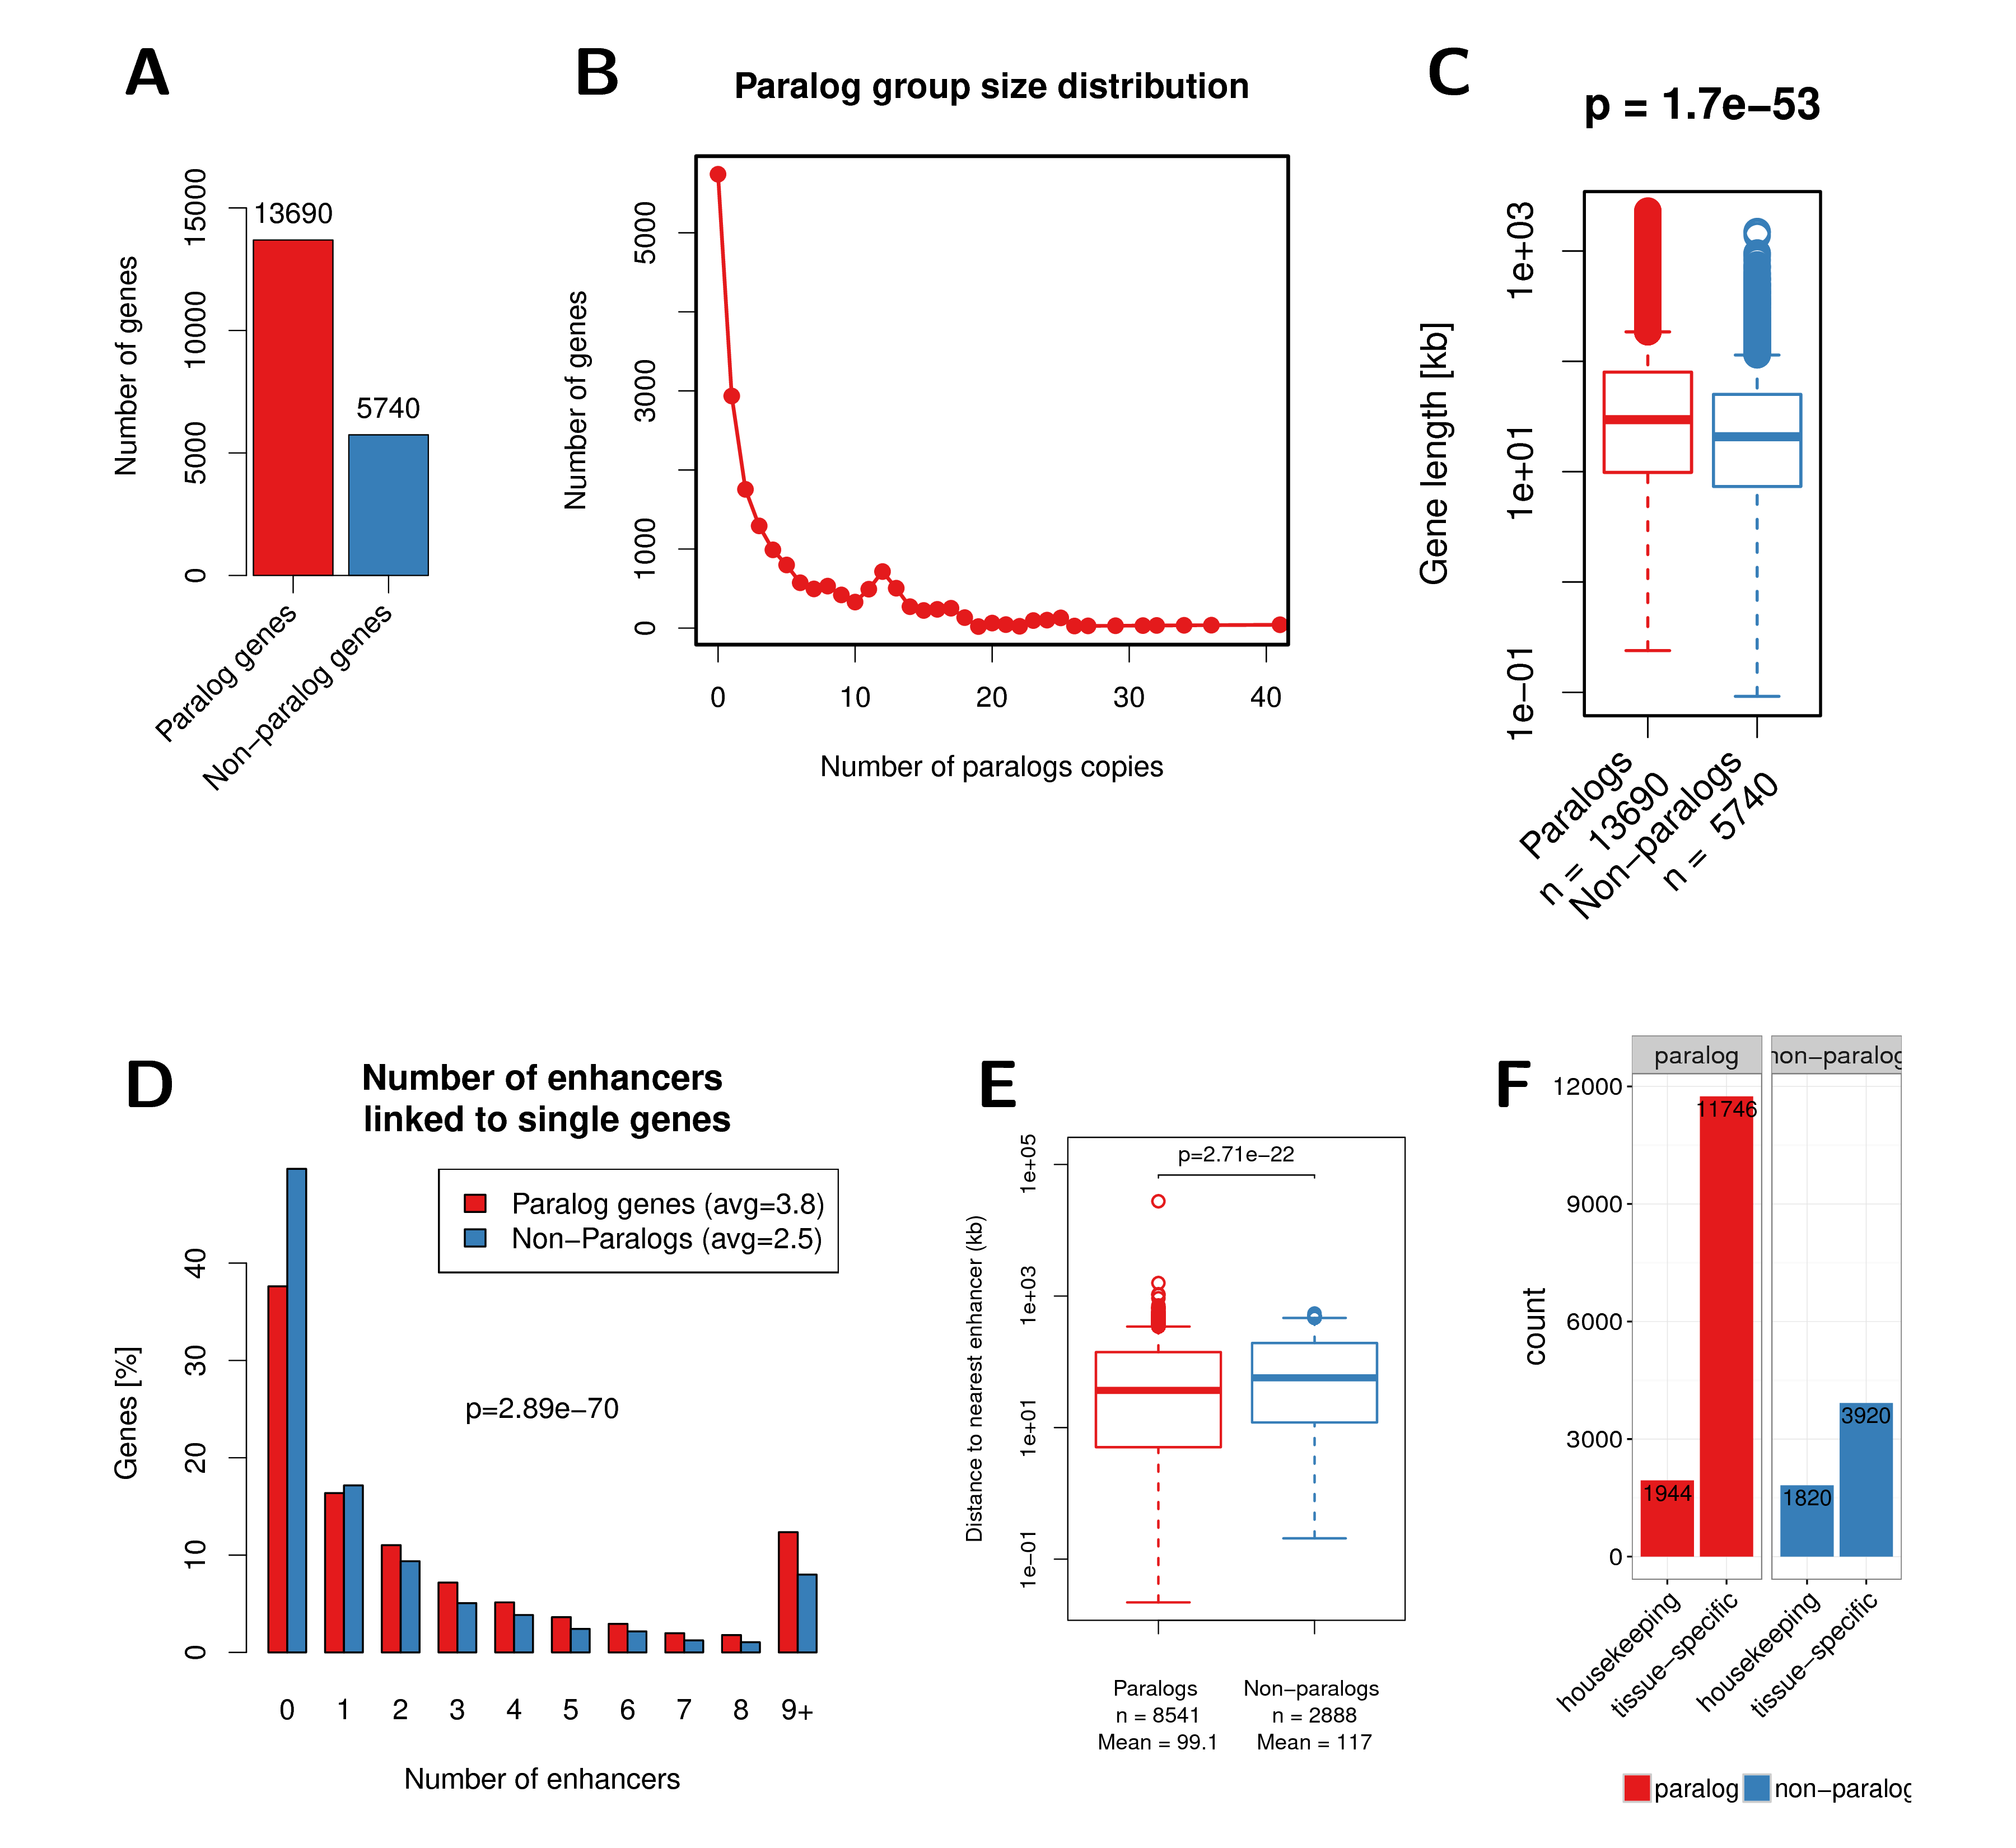
\includegraphics[width=0.5\linewidth]{figures/paralog/SI/figS1} 

}

\caption{\textbf{(A)} Number of paralog and non-paralog genes
in the human genome. \textbf{(B)} Paralog group size distribution in the
human genome. \textbf{(C)} Gene length of paralog and non-paralog genes.
\textbf{(D)} Distribution of the number of enhancers linked to single
genes compared between paralog genes (red) and non-paralog genes (blue).
\textbf{(E)} Genomic distance to nearest enhancer for paralogs and
non-paralog genes. \textbf{(F)} Number of housekeeping genes among
paralogs and non-paralog human genes. A recently published set of
housekeeping genes was used here \citep{Eisenberg2013}. The p-values
shown in this figure were calculated using the Wilcoxon rank-sum test.}\label{fig:paraVSnonPara}
\end{figure}












\begin{figure}

{\centering 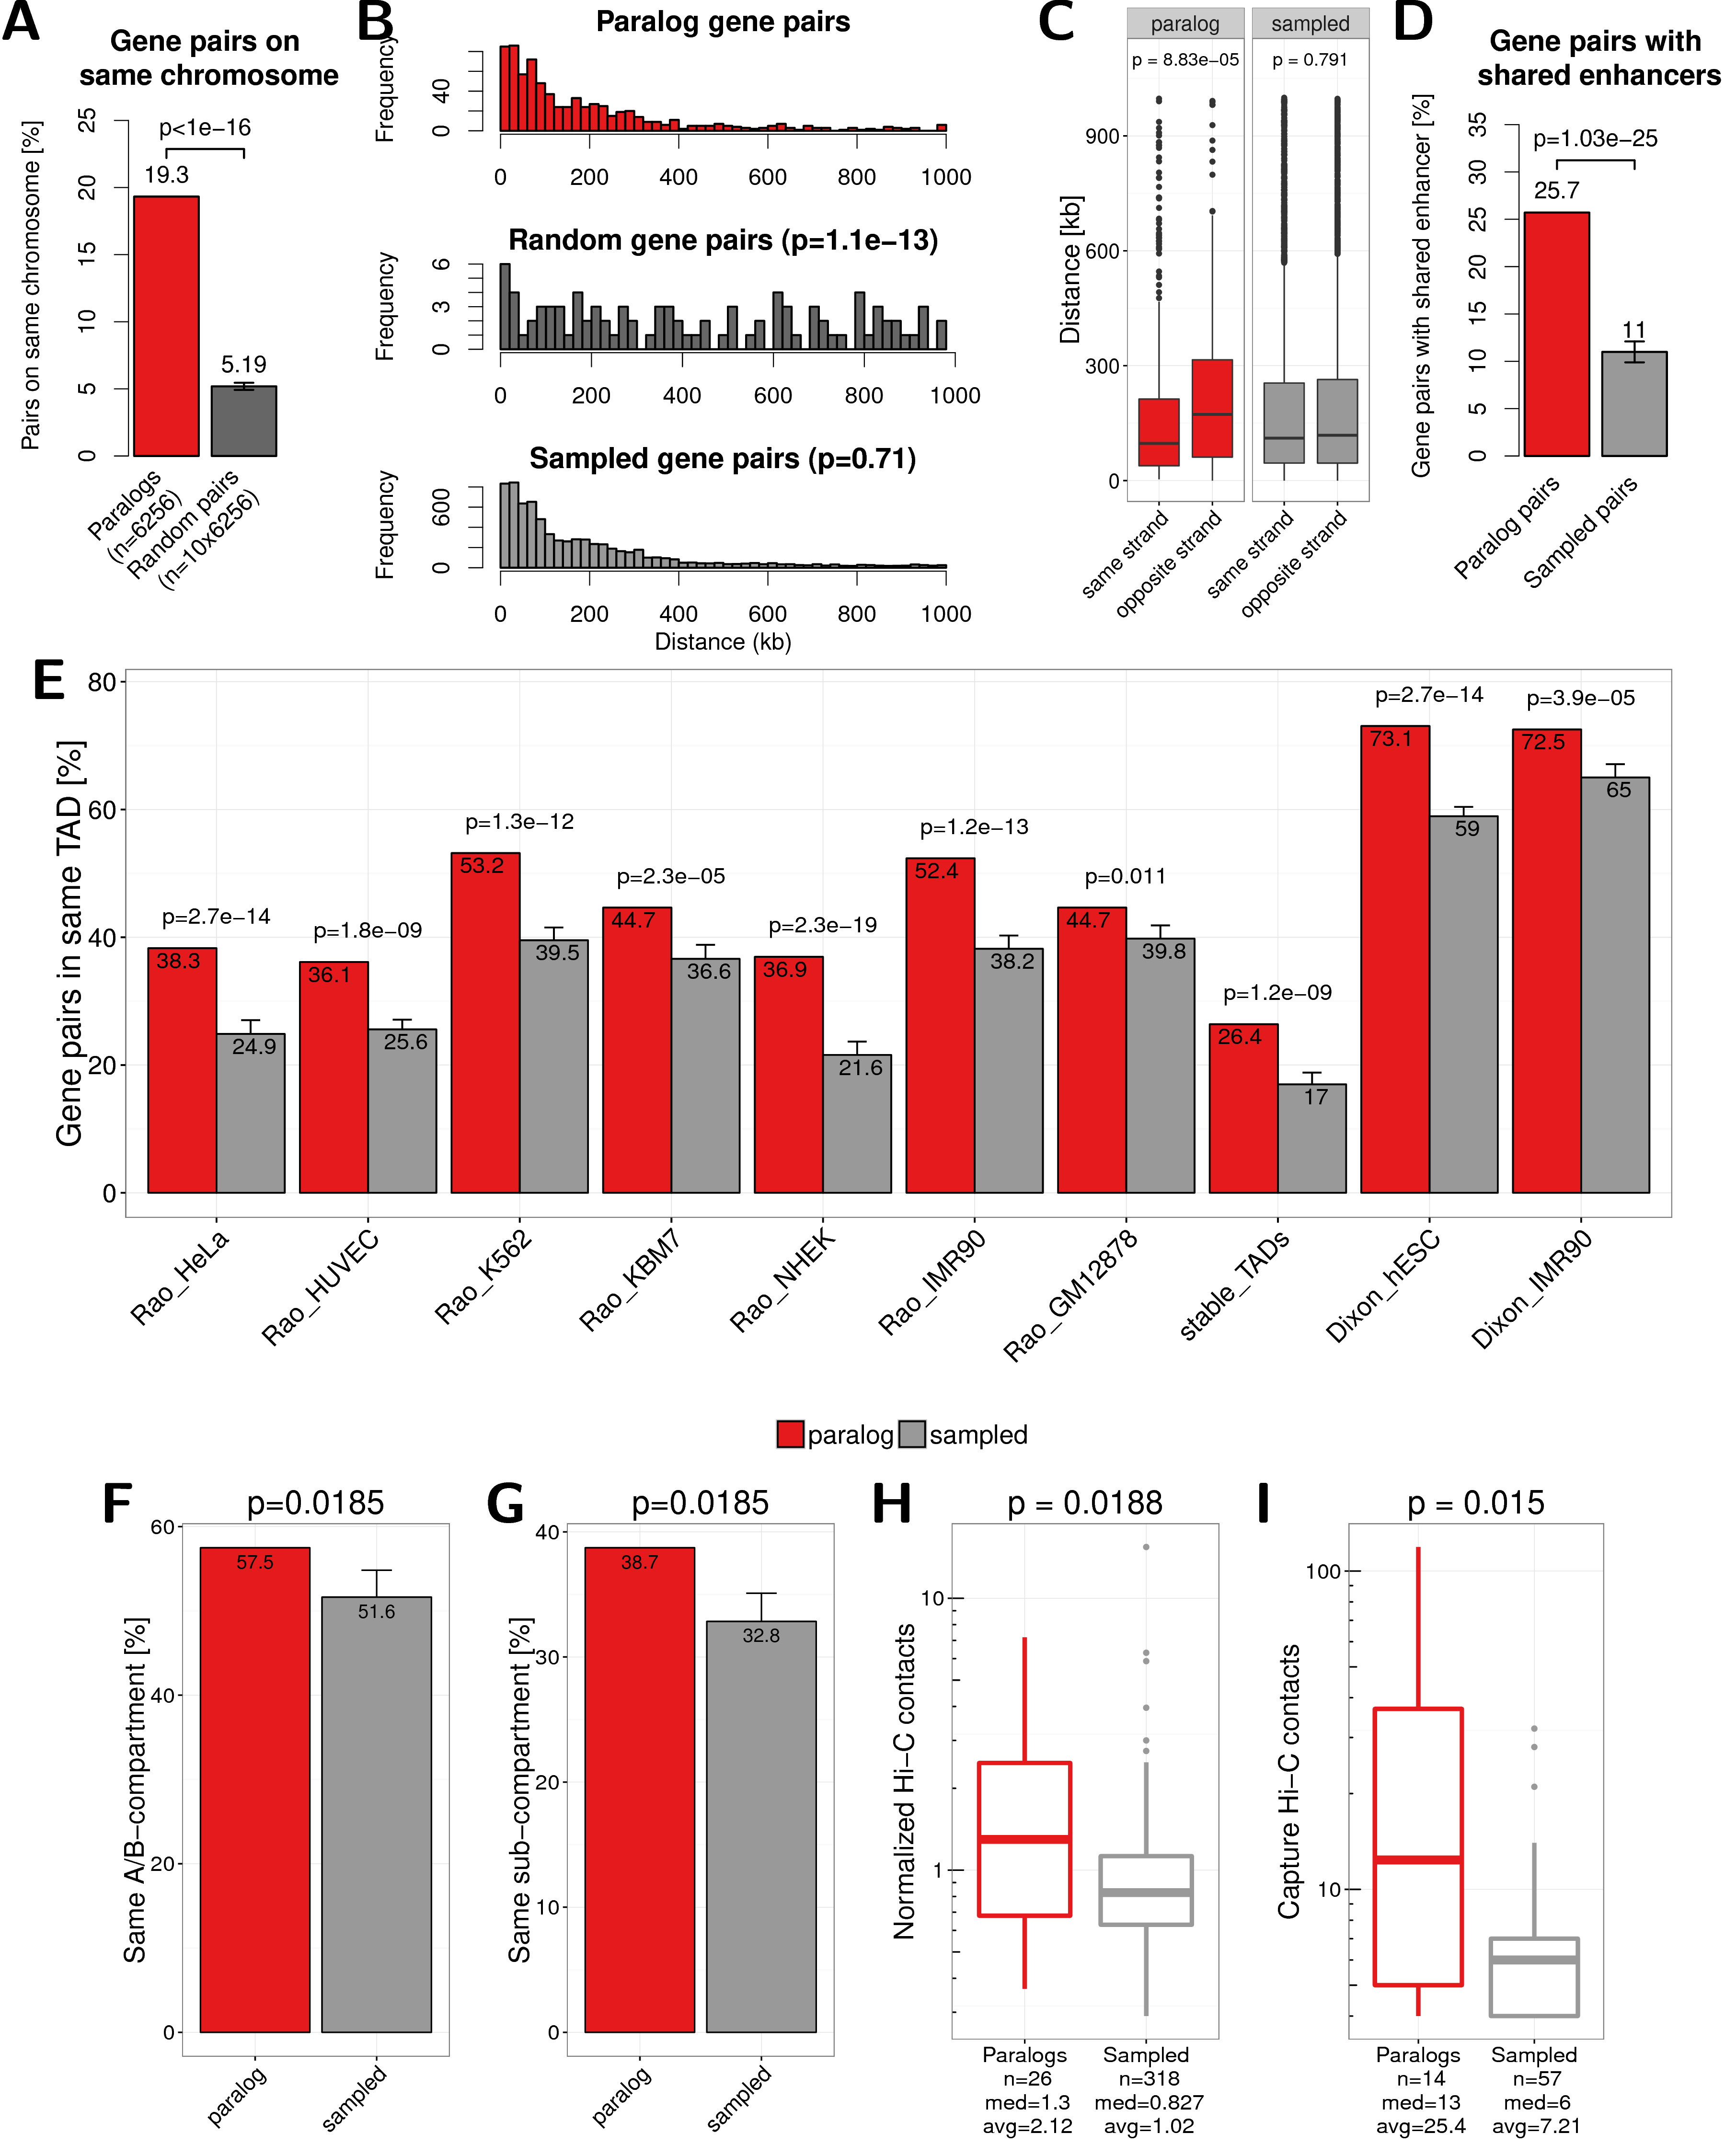
\includegraphics[width=0.5\linewidth]{figures/paralog/SI/figS2} 

}

\caption{Main results of this study by changing the
selection of paralog pairs from families with more than two paralogs.
Here pairs are selected by maximizing the rate of synonymous mutations
between them instead of minimizing, as in the main text. \textbf{(A)}
Percent of paralogs pairs on the same chromosome compared to random
pairs. \textbf{(B)} Distance distribution between pairs of paralogs
(red), random pairs (dark grey), and sampled pairs according to the
distances of paralogs (grey). \textbf{(C)} Genomic distance between
close paralogs and sampled pairs separated by same strand or not same
strand of gene pairs. \textbf{(D)} Percent of close paralogs and sampled
pairs with at least one shared enhancer. \textbf{(E)} Percent of close
gene pairs located within the same TAD for different TAD data sets.
\textbf{(F)} Percent of paralog and sampled pairs that are in the same
A/B compartment. \textbf{(G)} Percent of paralog and sampled pairs that
are in the same subcompartment. \textbf{(H)} Normalized Hi-C contacts
between distal paralogs and sampled genes. \textbf{(I)} Promoter
capture-C contacts between distal paralogs and sampled genes.}\label{fig:selectOldPairs}
\end{figure}



















\begin{figure}

{\centering 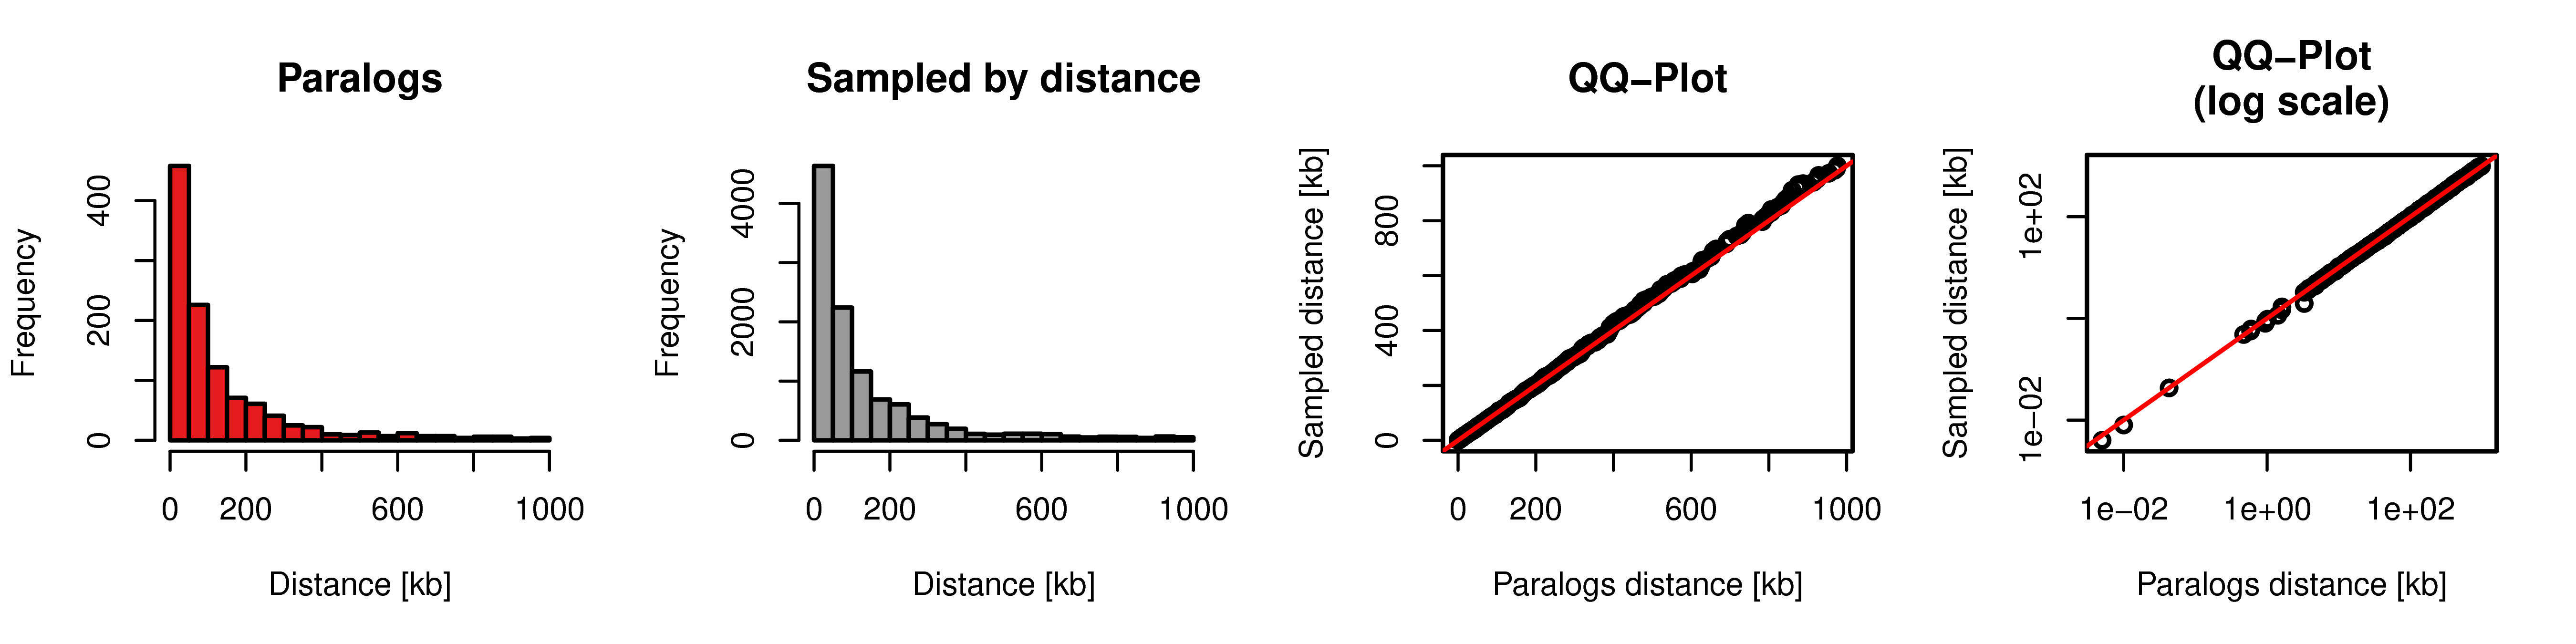
\includegraphics[width=0.5\linewidth]{figures/paralog/SI/figS3} 

}

\caption{\textbf{Sampling of gene pairs by distance.} Distance
distribution of paralog pairs (red) and sampled background gene pairs
(grey) and quantile-quantile plot of these two distributions in linear
axis (third column) and log scaled axis (fourth column).}\label{fig:samplingDist}
\end{figure}






\begin{figure}

{\centering 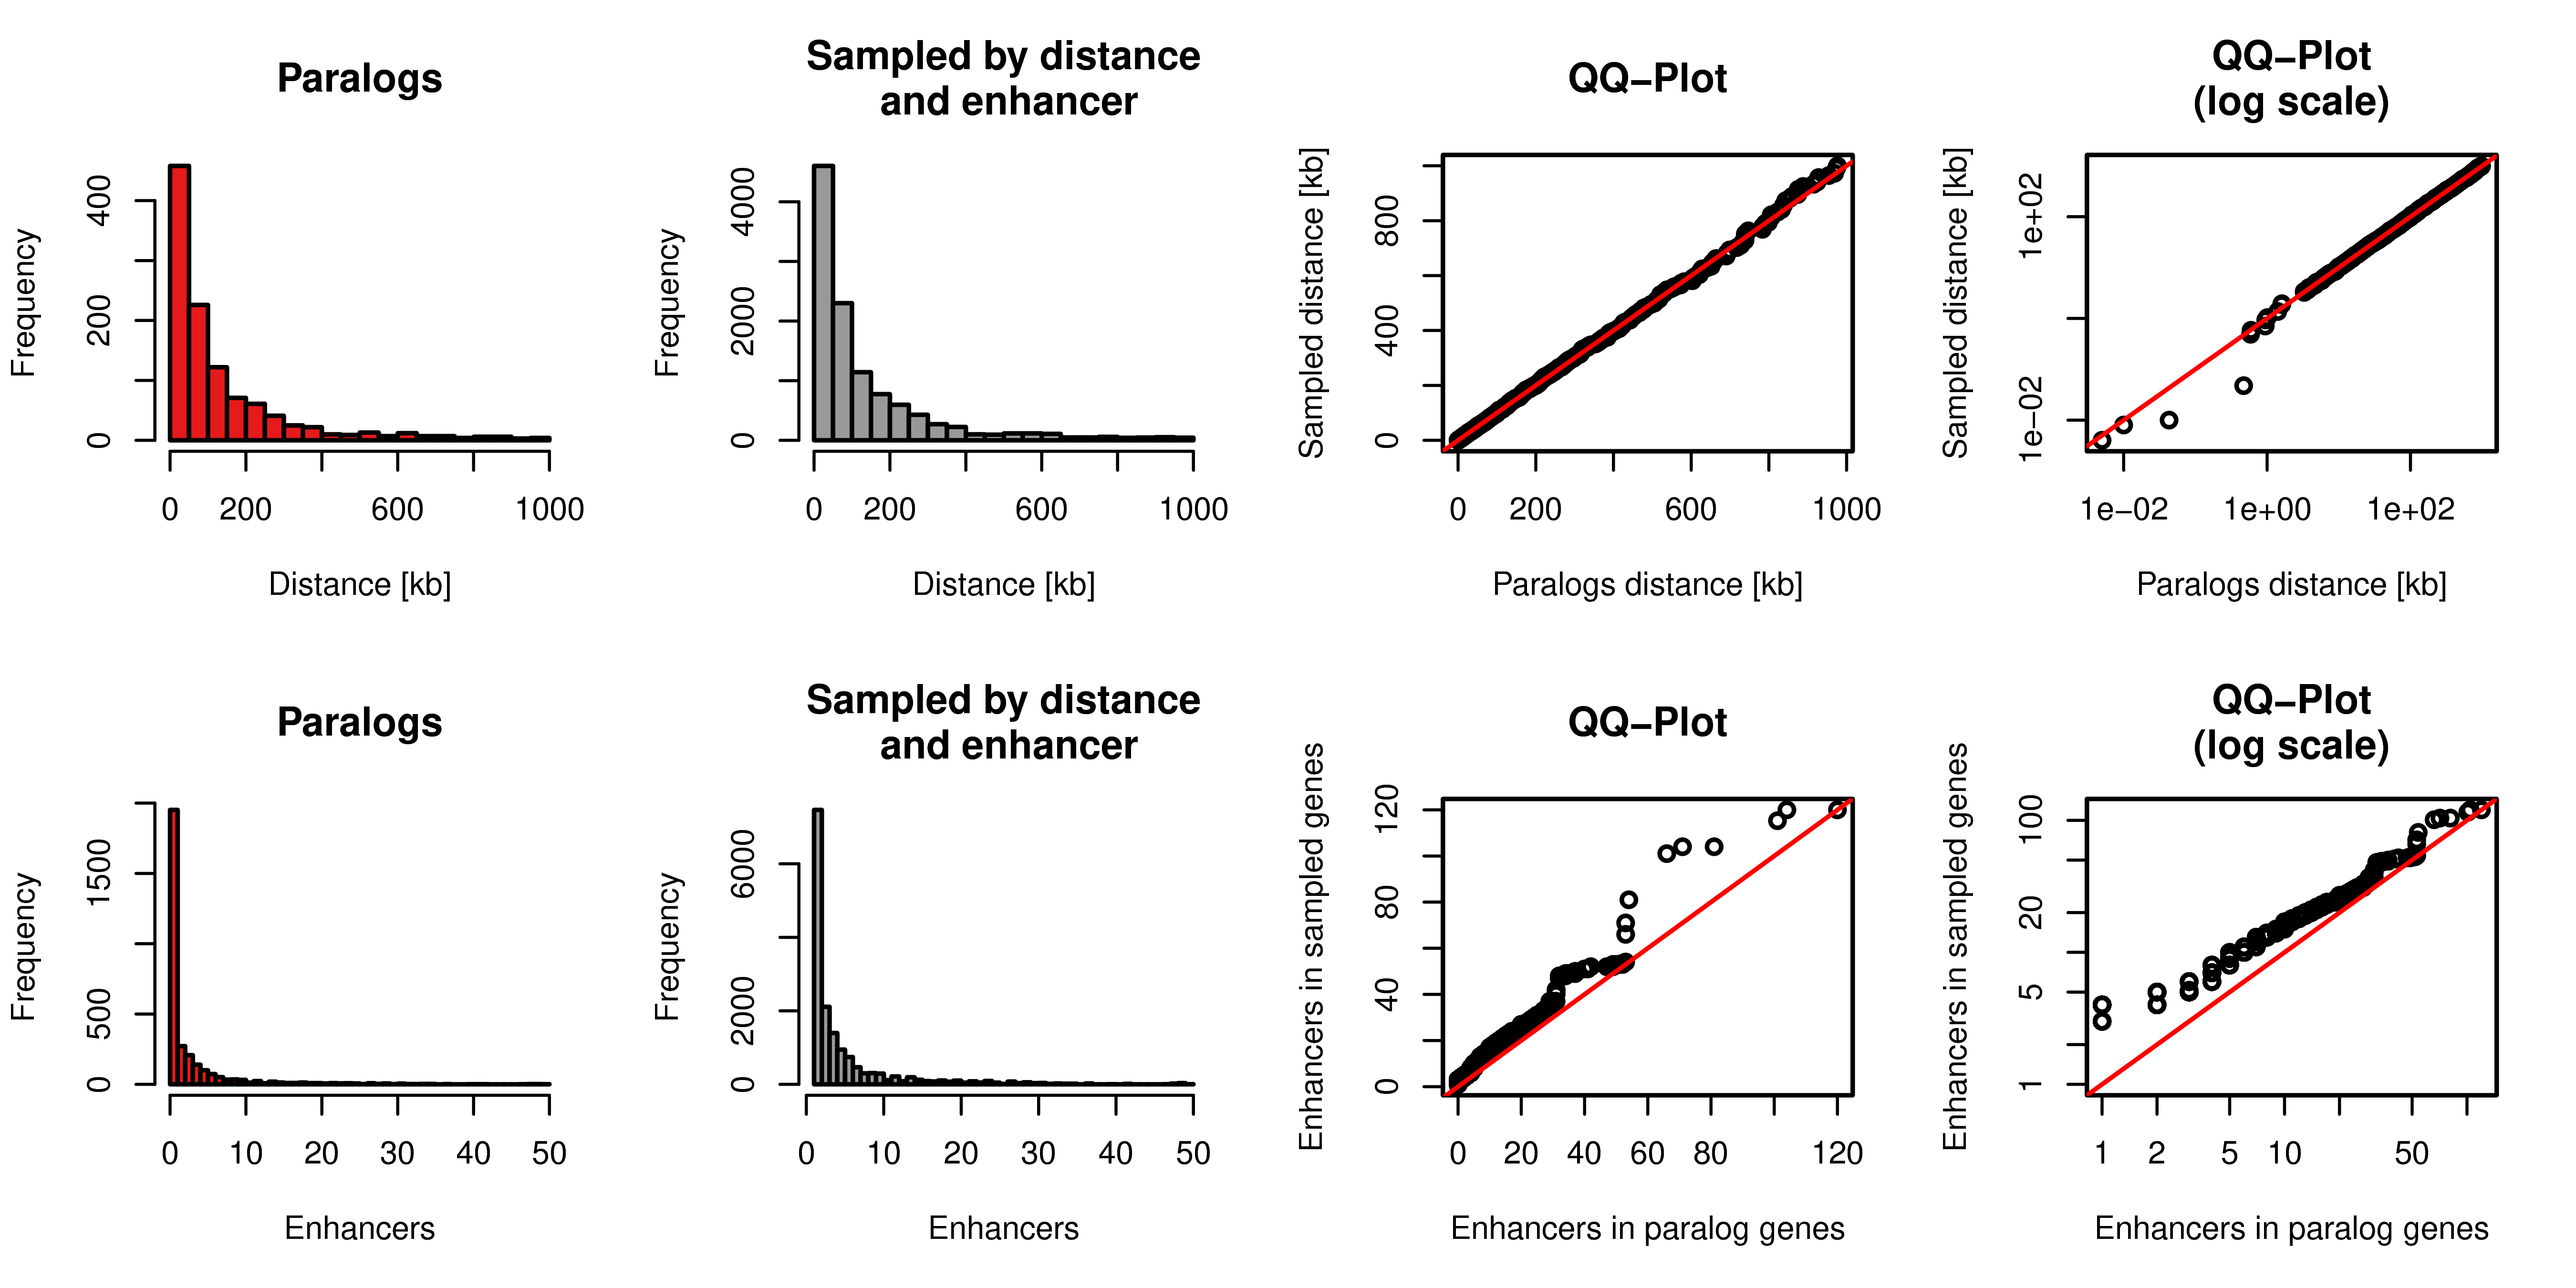
\includegraphics[width=0.5\linewidth]{figures/paralog/SI/figS4} 

}

\caption{\textbf{Sampling of gene pairs by distance and
number of enhancers.} Top row: Distance distribution of paralog pairs
(red) and sampled background gene pairs (grey) and quantile-quantile
plot of these two distributions in linear axis (third column) and log
scaled axis (fourth column). Bottom row: Distance of the number of
enhancers linked to each single gene in the pairs of paralogs (red) and
sampled background gene pairs (grey) and quantile-quantile plot of these
two distributions in linear axis (third column) and log scaled axis
(fourth column).}\label{fig:samplingDistEh}
\end{figure}











\begin{figure}

{\centering 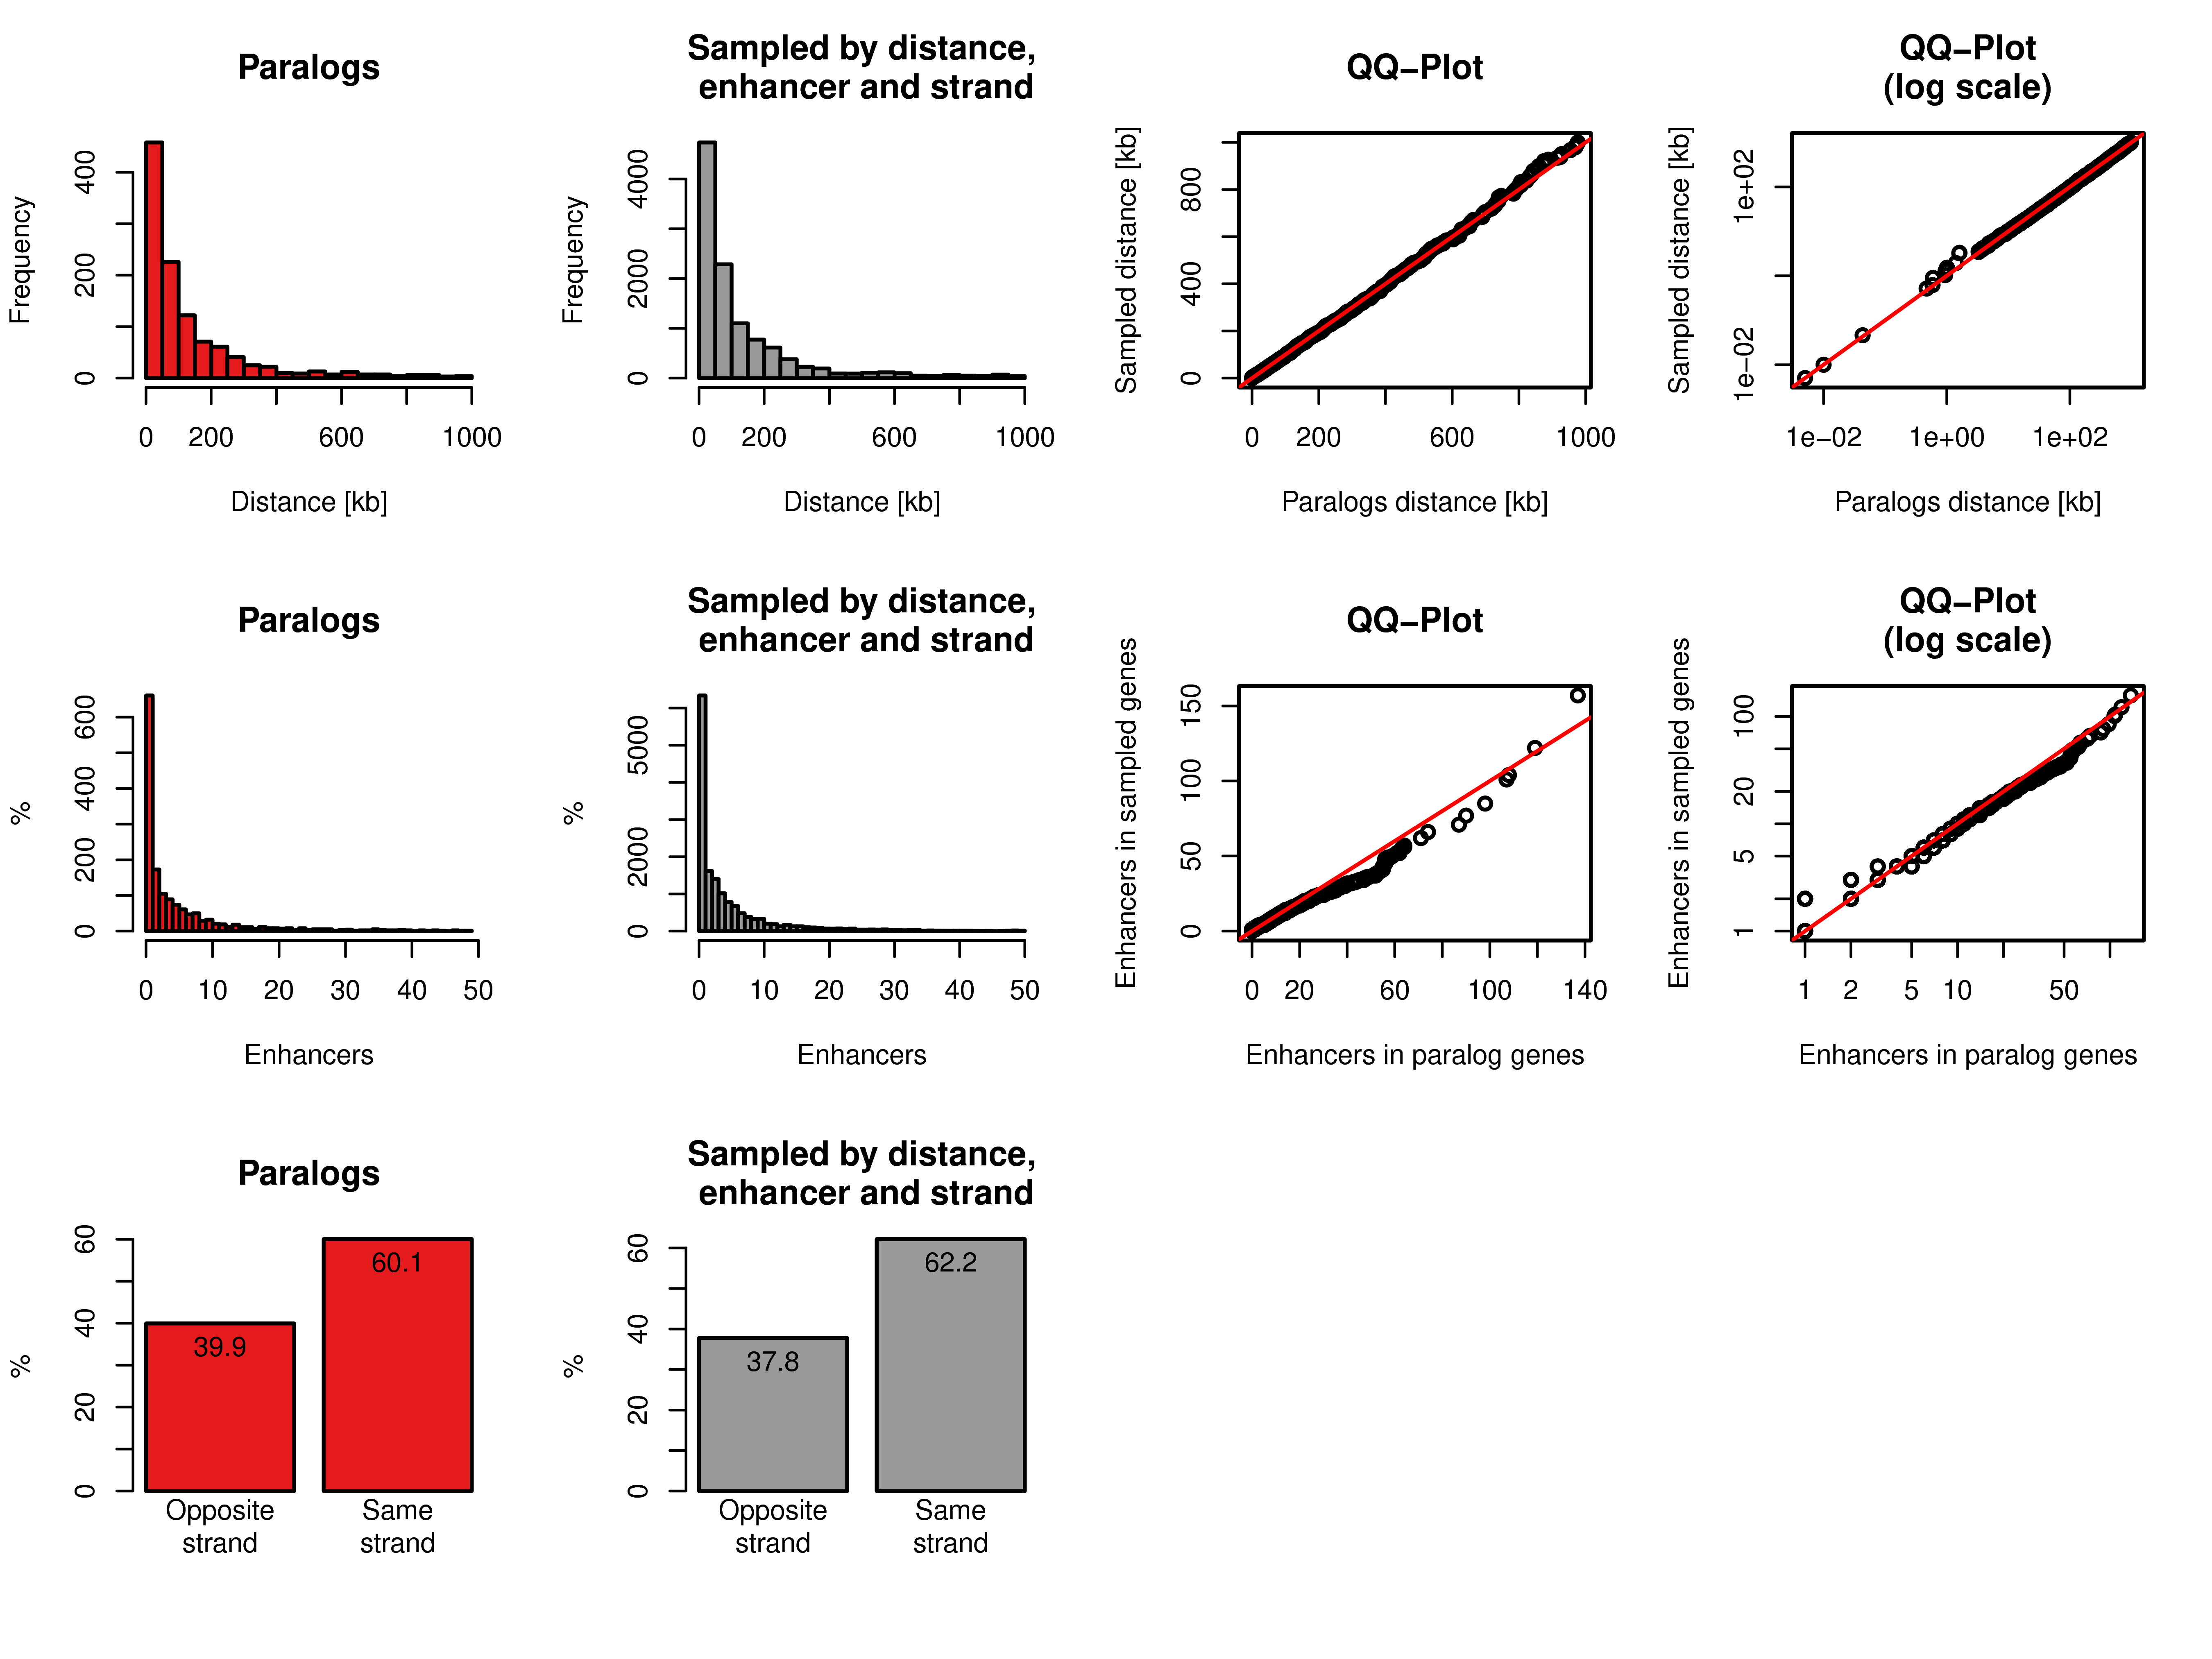
\includegraphics[width=0.5\linewidth]{figures/paralog/SI/figS5} 

}

\caption{\textbf{Sampling of gene pairs by distance,
number of enhancers, and same strand frequency.} Top row: Distance
distribution of paralog pairs (red) and sampled background gene pairs
(grey) and quantile-quantile plot of these two distributions in linear
axis (third column) and log scaled axis (fourth column). Middle row:
Distance of the number of enhancers linked to each single gene in the
pairs of paralogs (red) and sampled background gene pairs (grey) and
quantile-quantile plot of these two distributions in linear axis (third
column) and log scaled axis (fourth column). Bottom row: Percentages of
pairs of genes with opposite or same strand of transcription for paralog
pairs (red) and sampled pairs (grey).}\label{fig:samplingDistEhStrand}
\end{figure}













\begin{figure}

{\centering 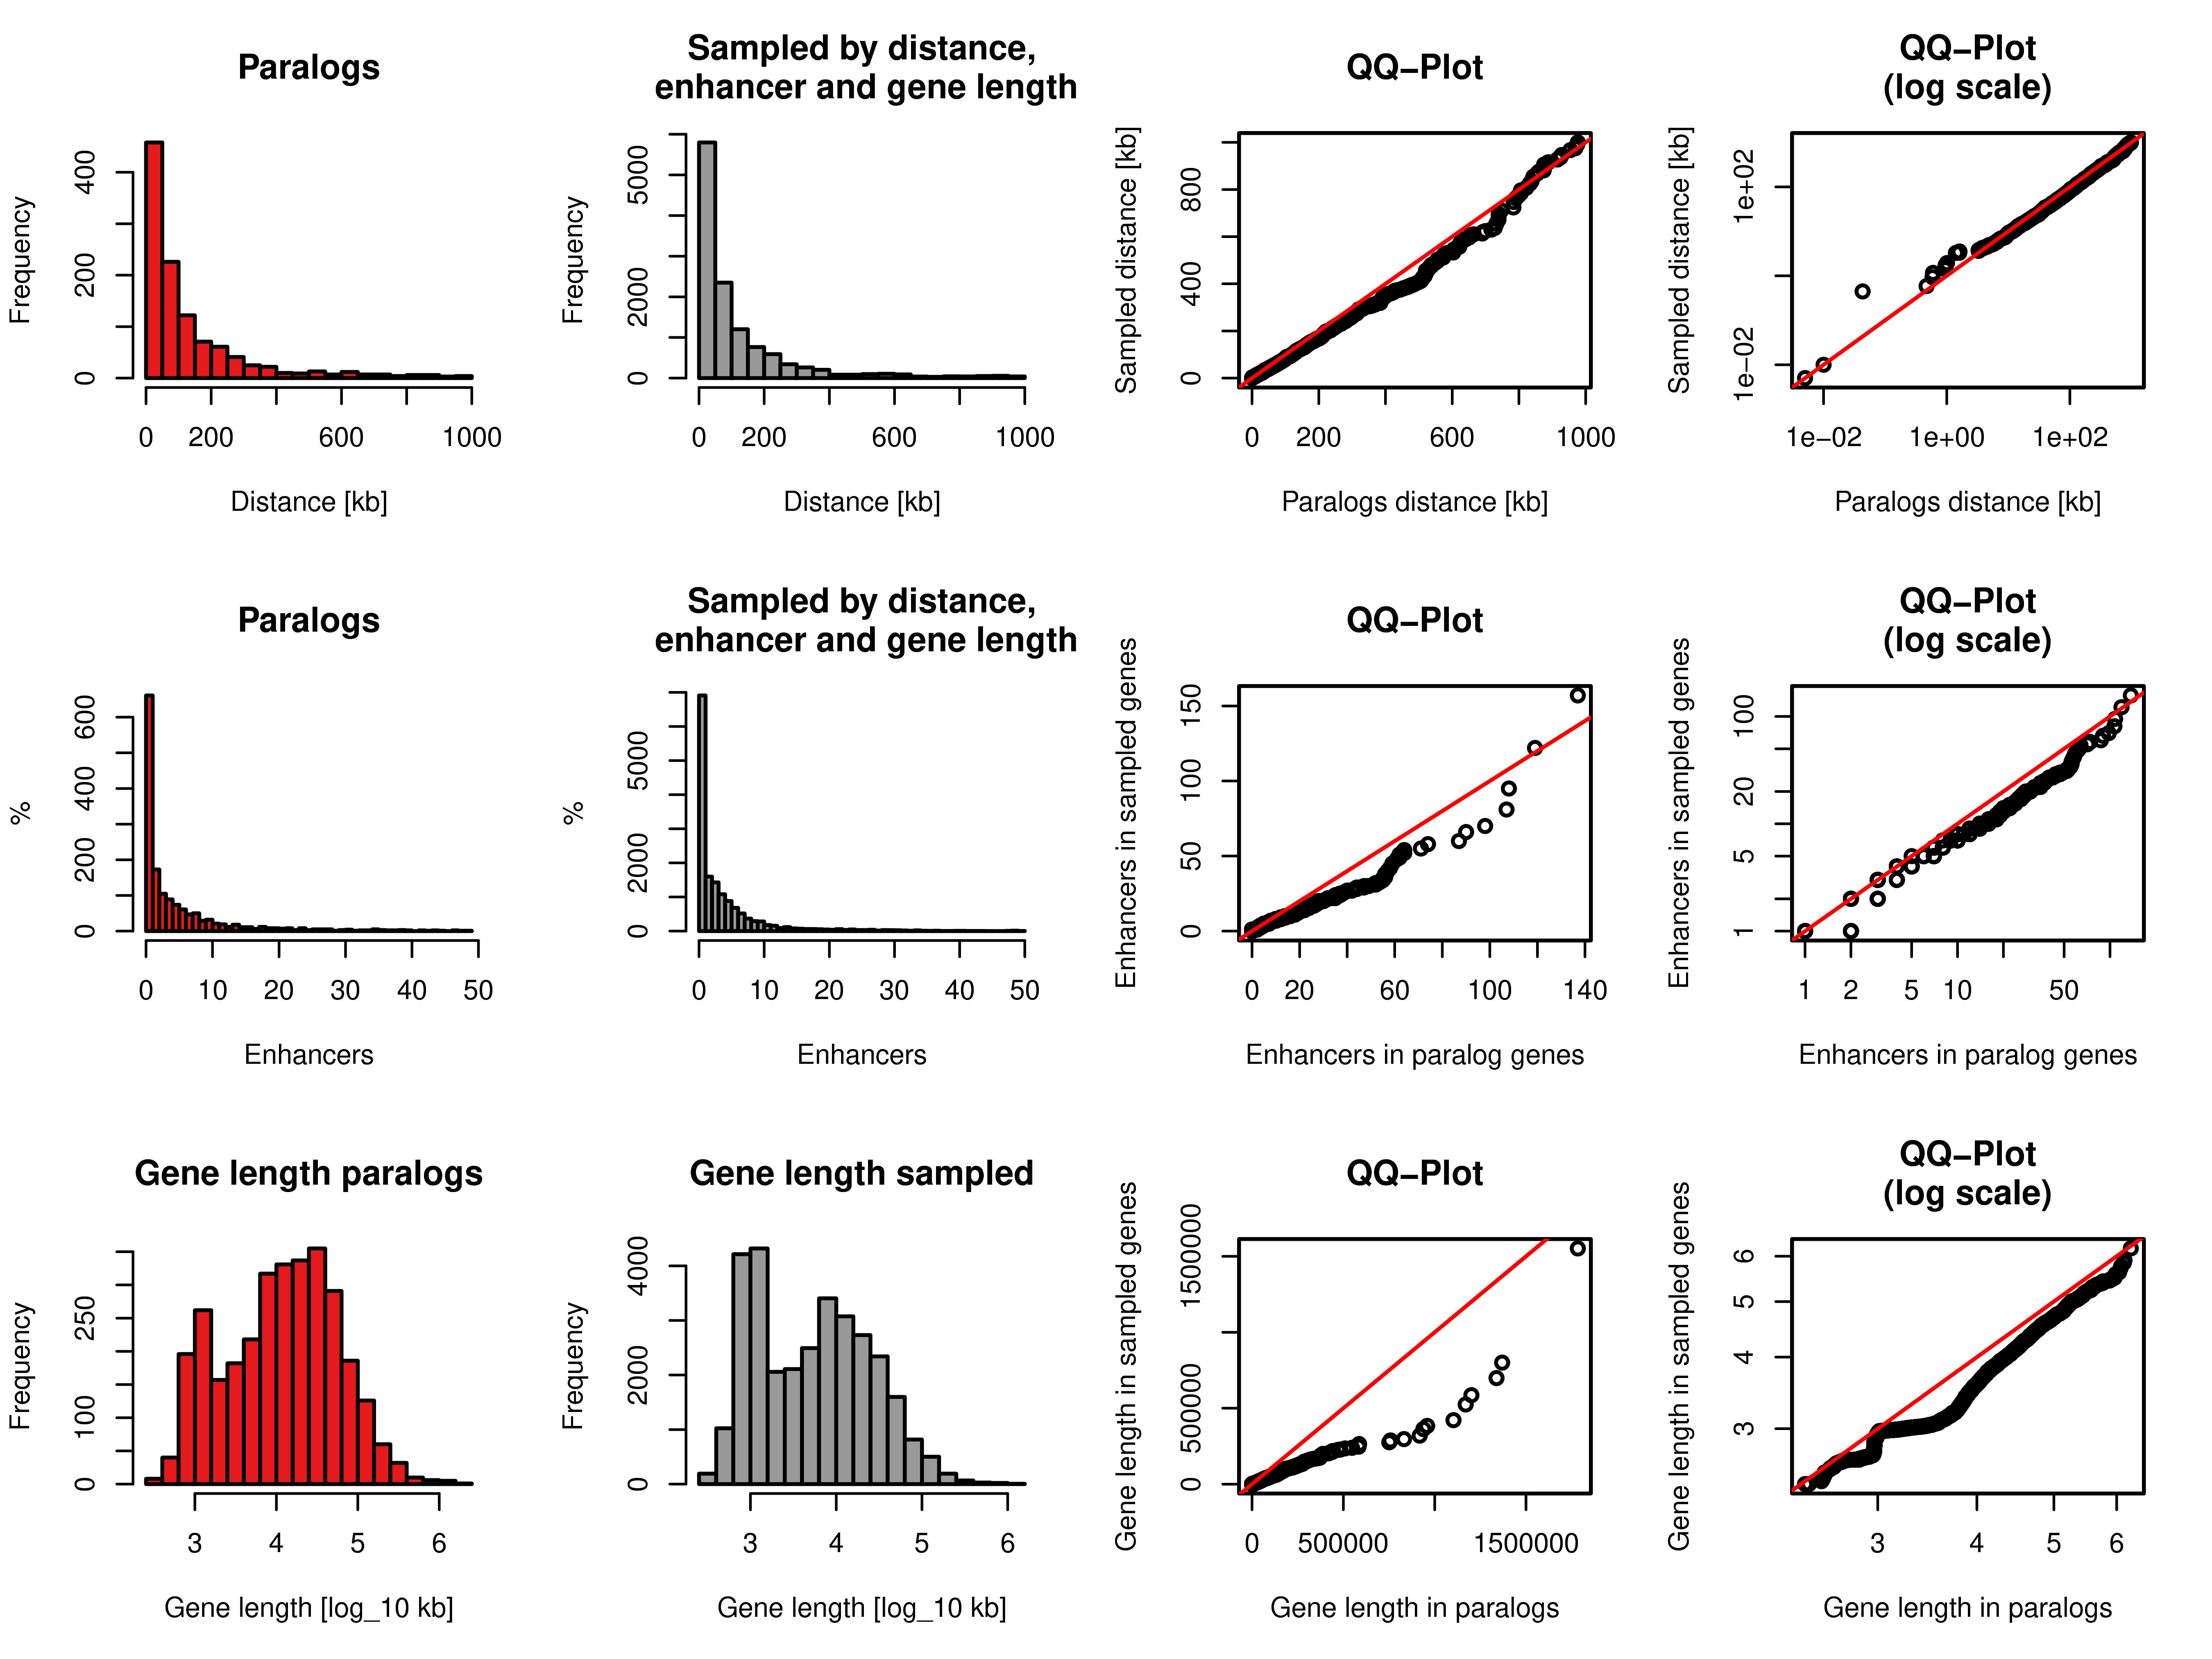
\includegraphics[width=0.5\linewidth]{figures/paralog/SI/figS6} 

}

\caption{\textbf{Sampling of gene pairs by distance,
number of enhancers, and same strand frequency.} Top row: Distance
distribution of paralog pairs (red) and sampled background gene pairs
(grey) and quantile-quantile plot of these two distributions in linear
axis (third column) and log scaled axis (fourth column). Middle row:
Distance of the number of enhancers linked to each single gene in the
pairs of paralogs (red) and sampled background gene pairs (grey) and
quantile-quantile plot of these two distributions in linear axis (third
column) and log scaled axis (fourth column). Bottom row: Distribution of
gene lengths of each single gene in the pairs of paralogs (red) and
sampled background gene pairs (grey) and quantile-quantile plot of these
two distributions in linear axis (third column) and \(\log_{10}\) of
gene lengths (fourth column).}\label{fig:samplingDistEhLen}
\end{figure}















\begin{figure}

{\centering 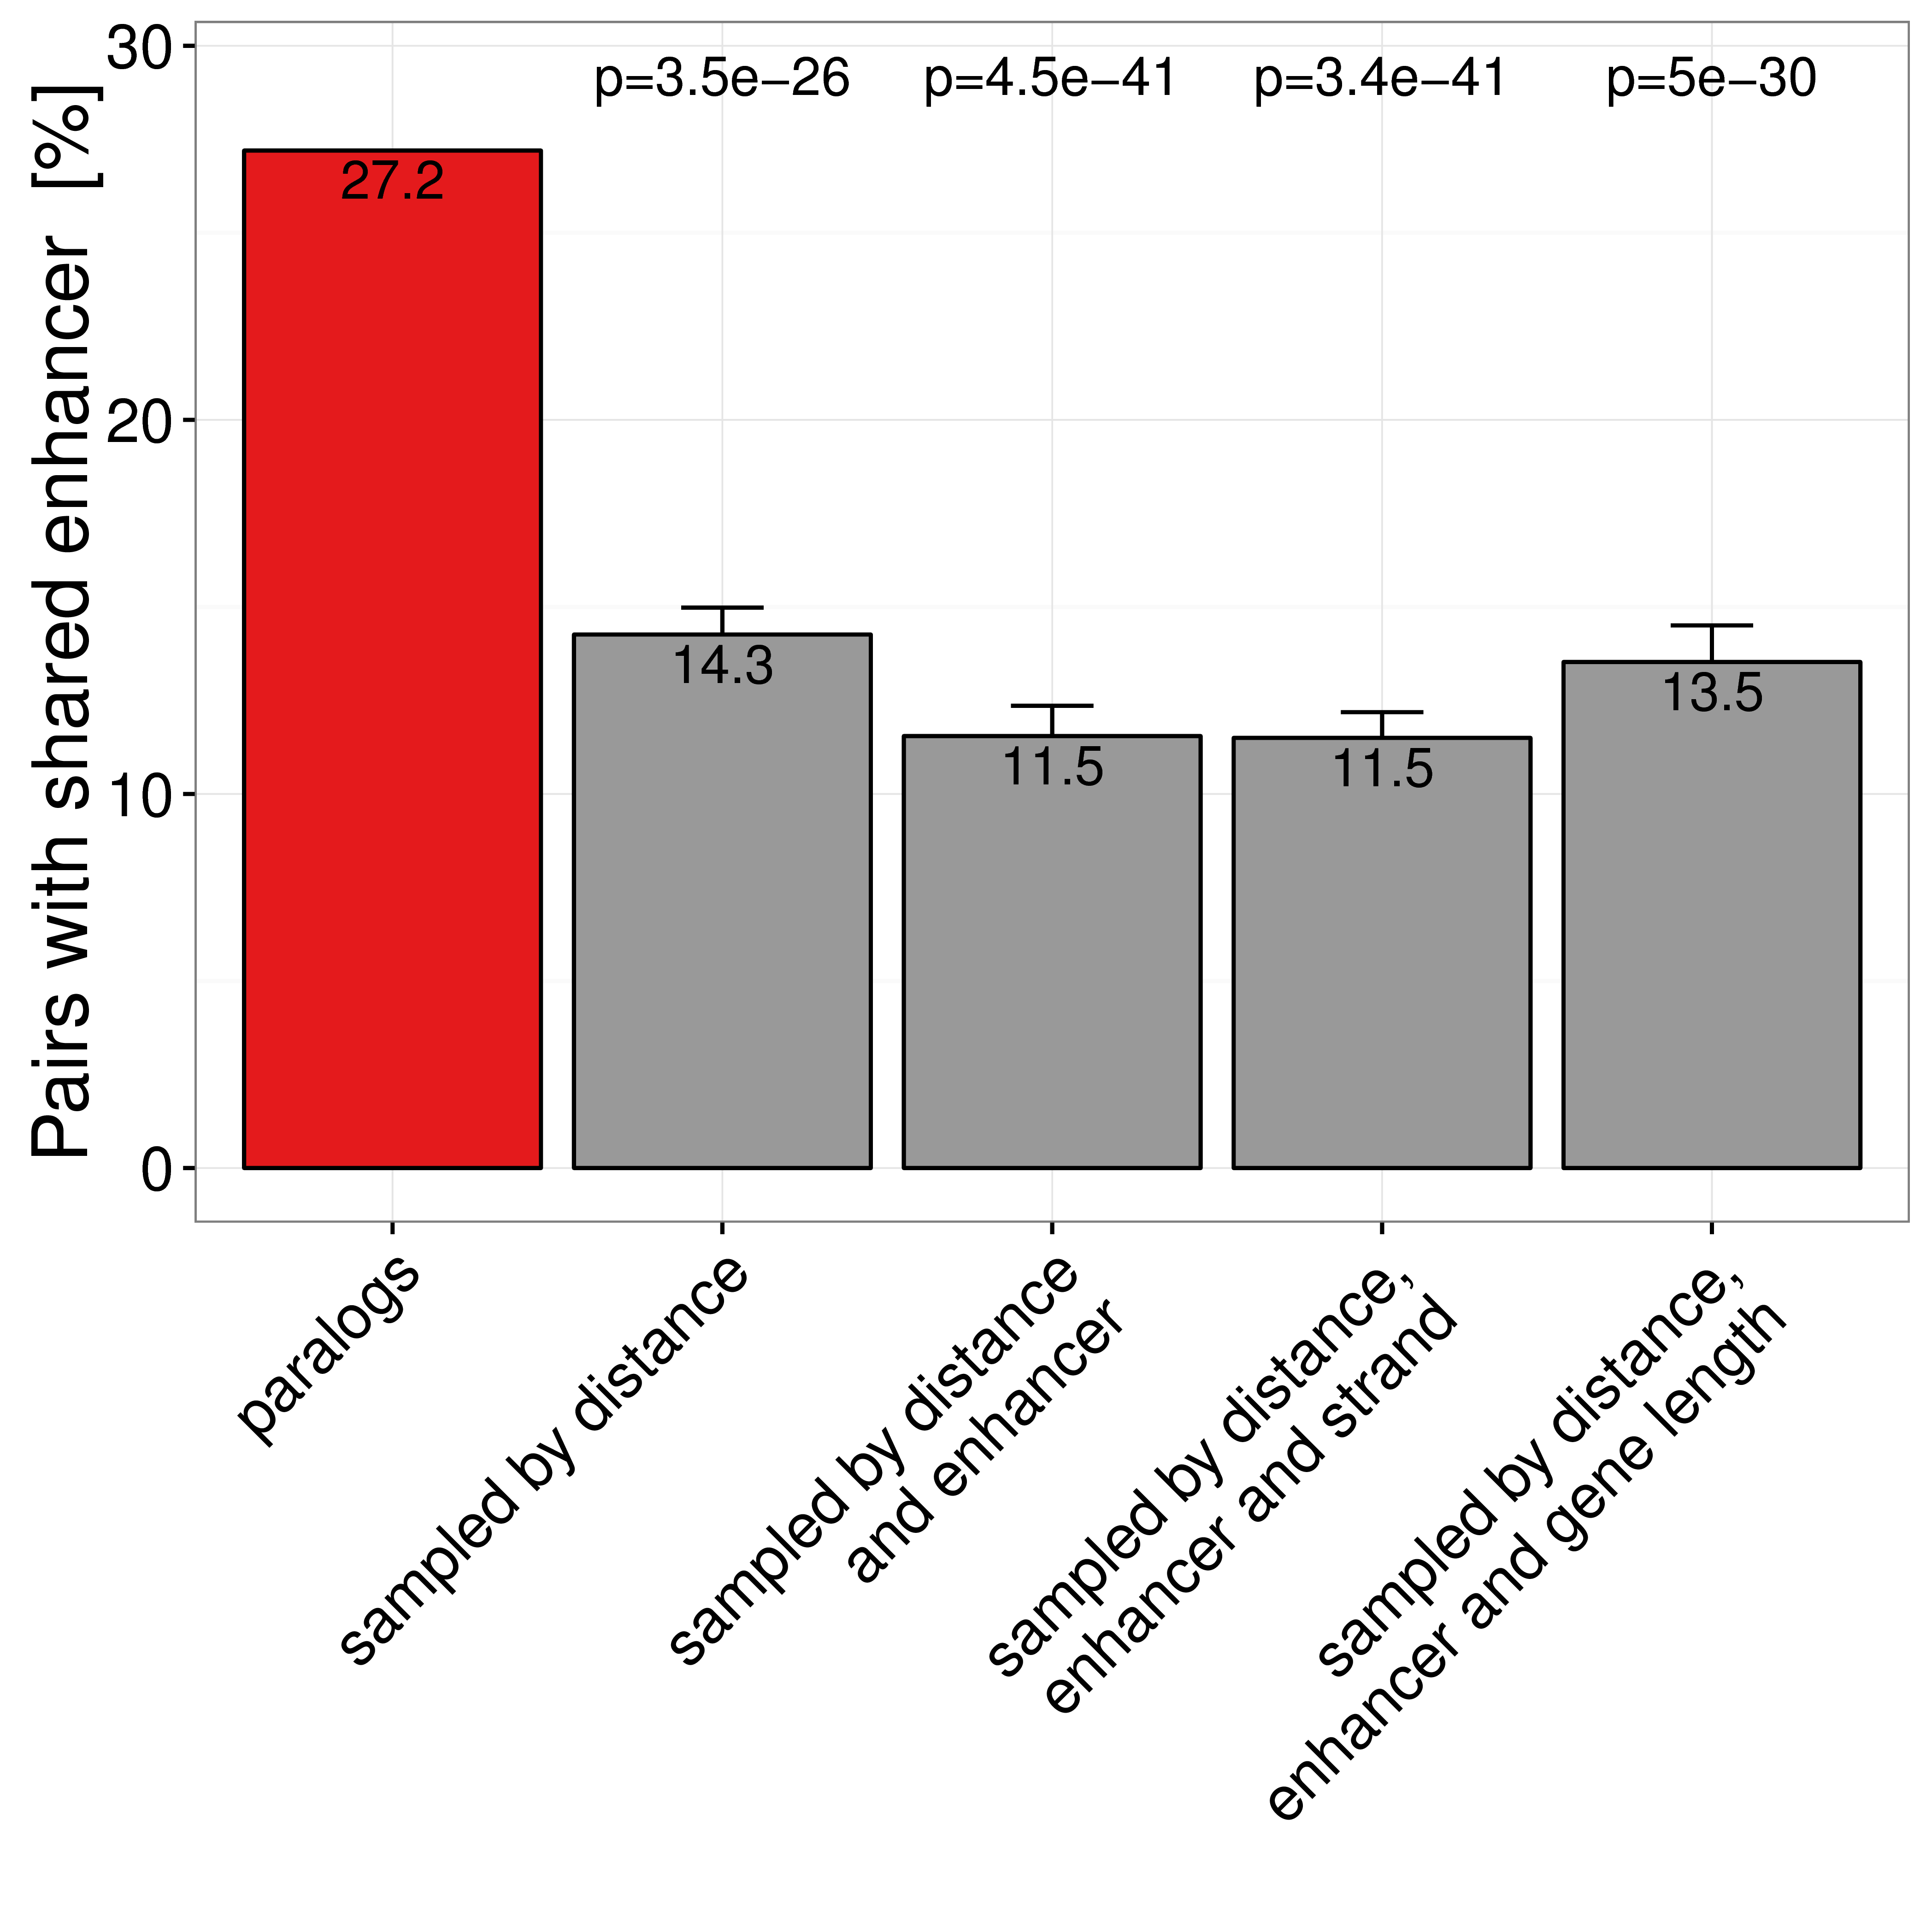
\includegraphics[width=0.5\linewidth]{figures/paralog/SI/figS7} 

}

\caption{Percent of gene pairs with at least one shared
enhancer in paralog pairs and four different types of sampled gene
pairs. Only pairs with TSS distance \(\leq\) 1Mb are considered. Error
bars indicate standard variation of ten times replicated sampling.}\label{fig:ehBySampType}
\end{figure}






\begin{figure}

{\centering 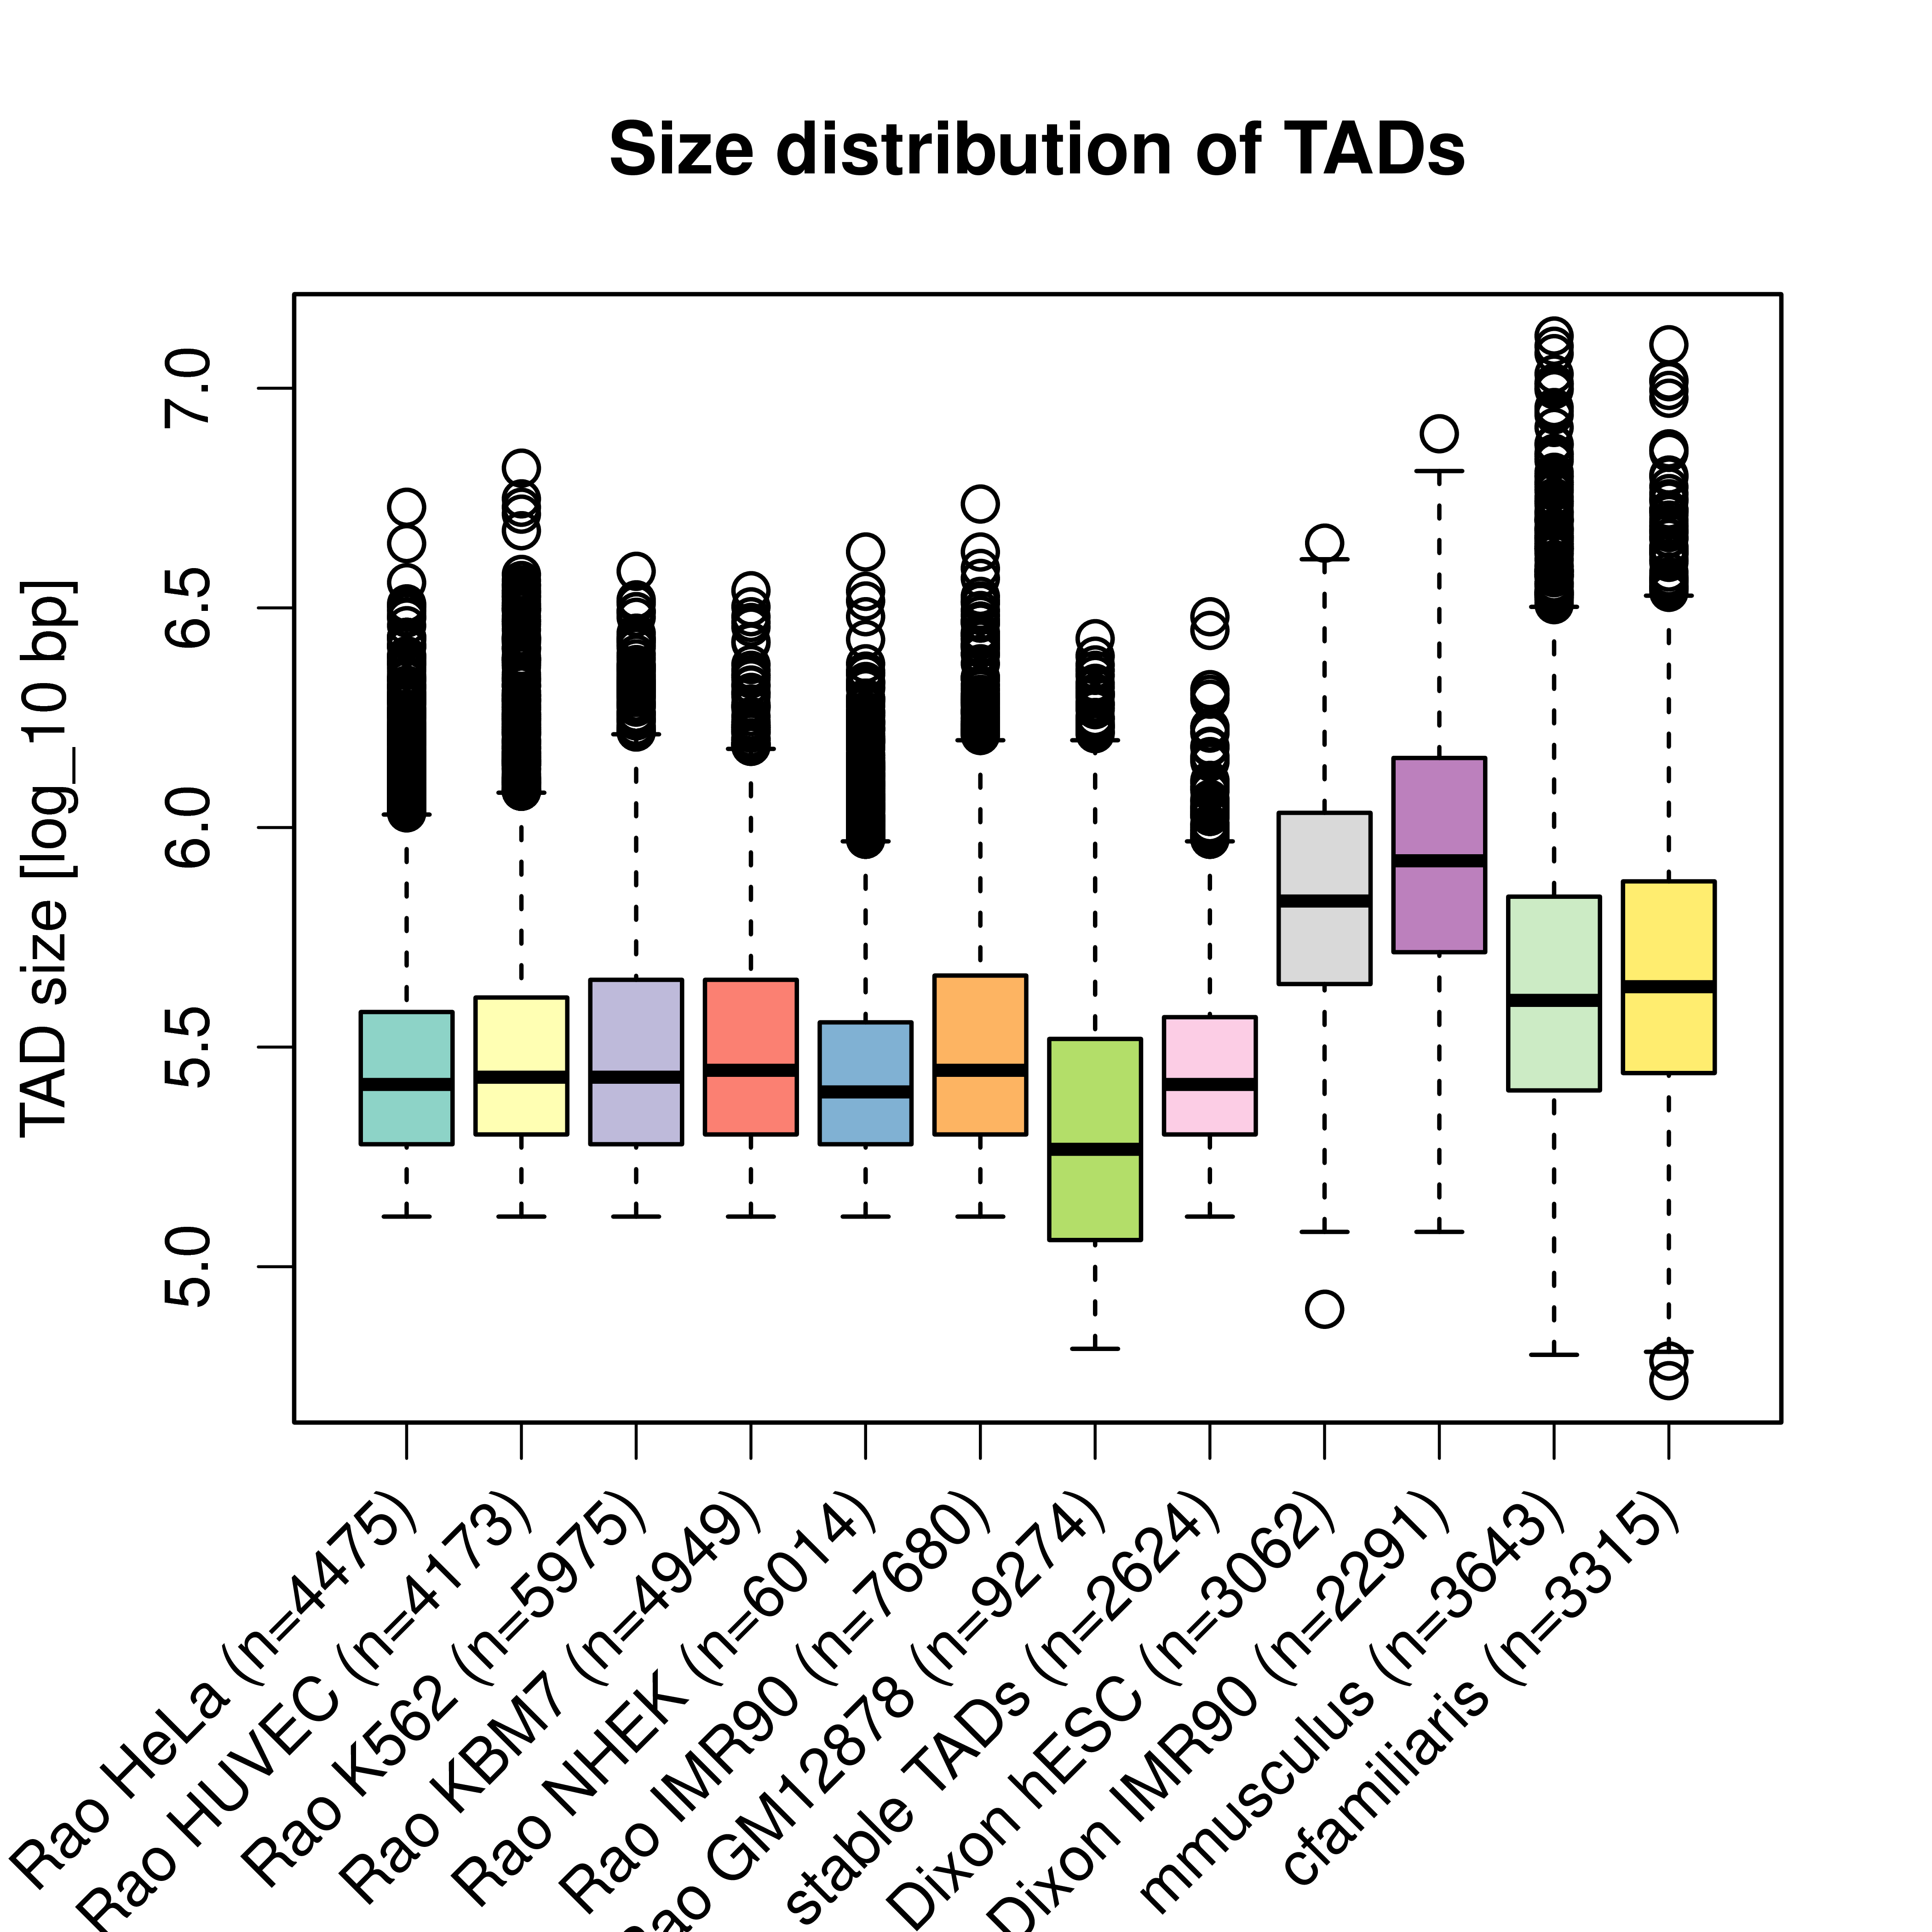
\includegraphics[width=0.5\linewidth]{figures/paralog/SI/figS8} 

}

\caption{\textbf{Size distribution of TADs in different cell-types,
studies, and species.} Each box shows the size-distribution of one data
set of TADs. The labels indicate the study (Rao \citep{Rao2014}, or
Dixon \citep{Dixon2012}), cell type and number of TADs in each data set.
The last two boxes are for TADs from Hi-C experiments in mouse and dog
Hi-C liver cells \citep{VietriRudan2015}.}\label{fig:TADsize}
\end{figure}








\begin{figure}

{\centering 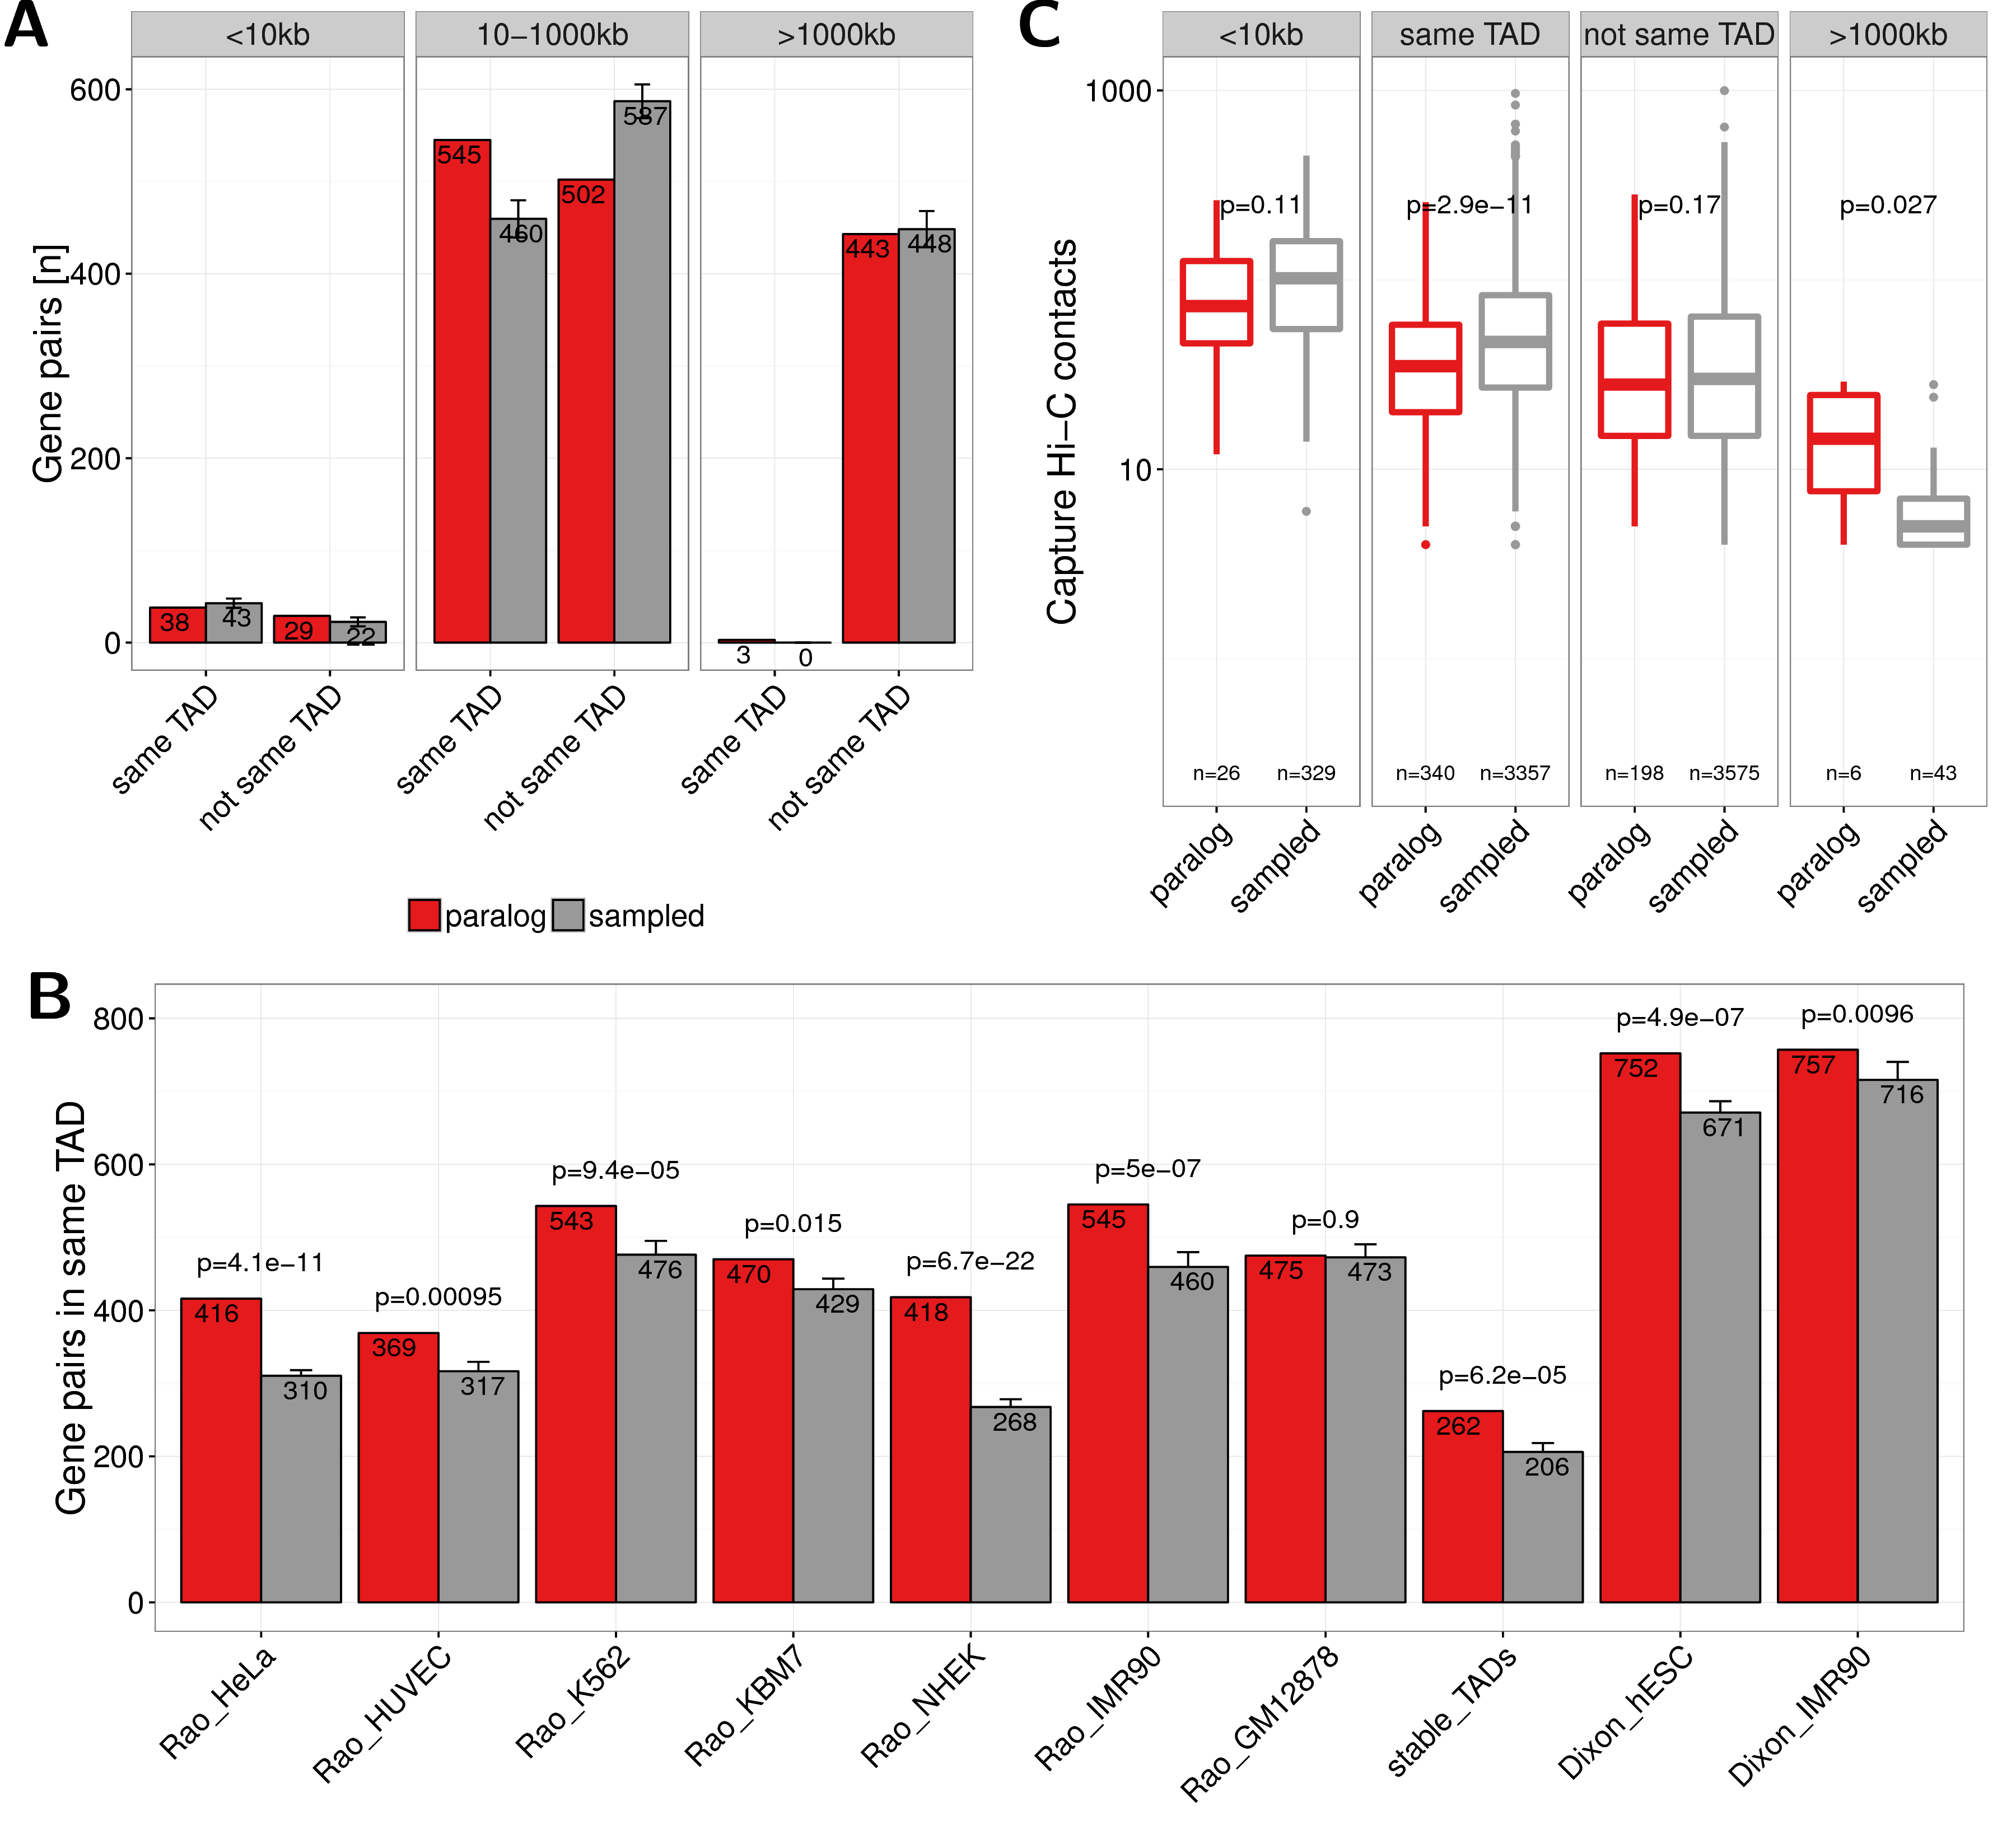
\includegraphics[width=0.5\linewidth]{figures/paralog/SI/figS9} 

}

\caption{\textbf{(A)} Number of paralog (red) and sampled
(grey) gene pairs that are in the same TAD or not separated in three
groups of genomic distances (0-10kb, 10-1000kb and \(>\) 1000kb). TADs
called from IMR90 cells by \citep{Rao2014} were used here. \textbf{(B)}
Co-localization of gene pairs with genomic distances between 10kb and
1000kb within the same TAD for paralogs and sampled gene pairs and
separated by TAD data sets from different cell types and studies. The
first seven bars show values for TADs called in HeLa, HUVEC, K562, KBM7,
NHEK, IMR90, and GM12878 cells by \citep{Rao2014}. The eighth bar shows
the value for stable TADs across cell types form this study (at least
90\% reciprocal overlap in 50\% of cells). The last two bars show data
for TADs called in hESC and IMR90 cells by \citep{Dixon2012}. Error bars
indicate standard deviation in 10 times replicated sampling of gene
pairs. P-values are computed using Fisher's exact test. \textbf{(C)}
Promoter capture-C contacts between pairs of paralogs (red) and sampled
gene pairs (grey) for the groups: \$\textless{}\$10kb genomic distance,
located in the same TAD, not in the same TAD, and with genomic distance
\$\textgreater{}\$1000kb.}\label{fig:closePairsInTAD}
\end{figure}




















\begin{figure}

{\centering 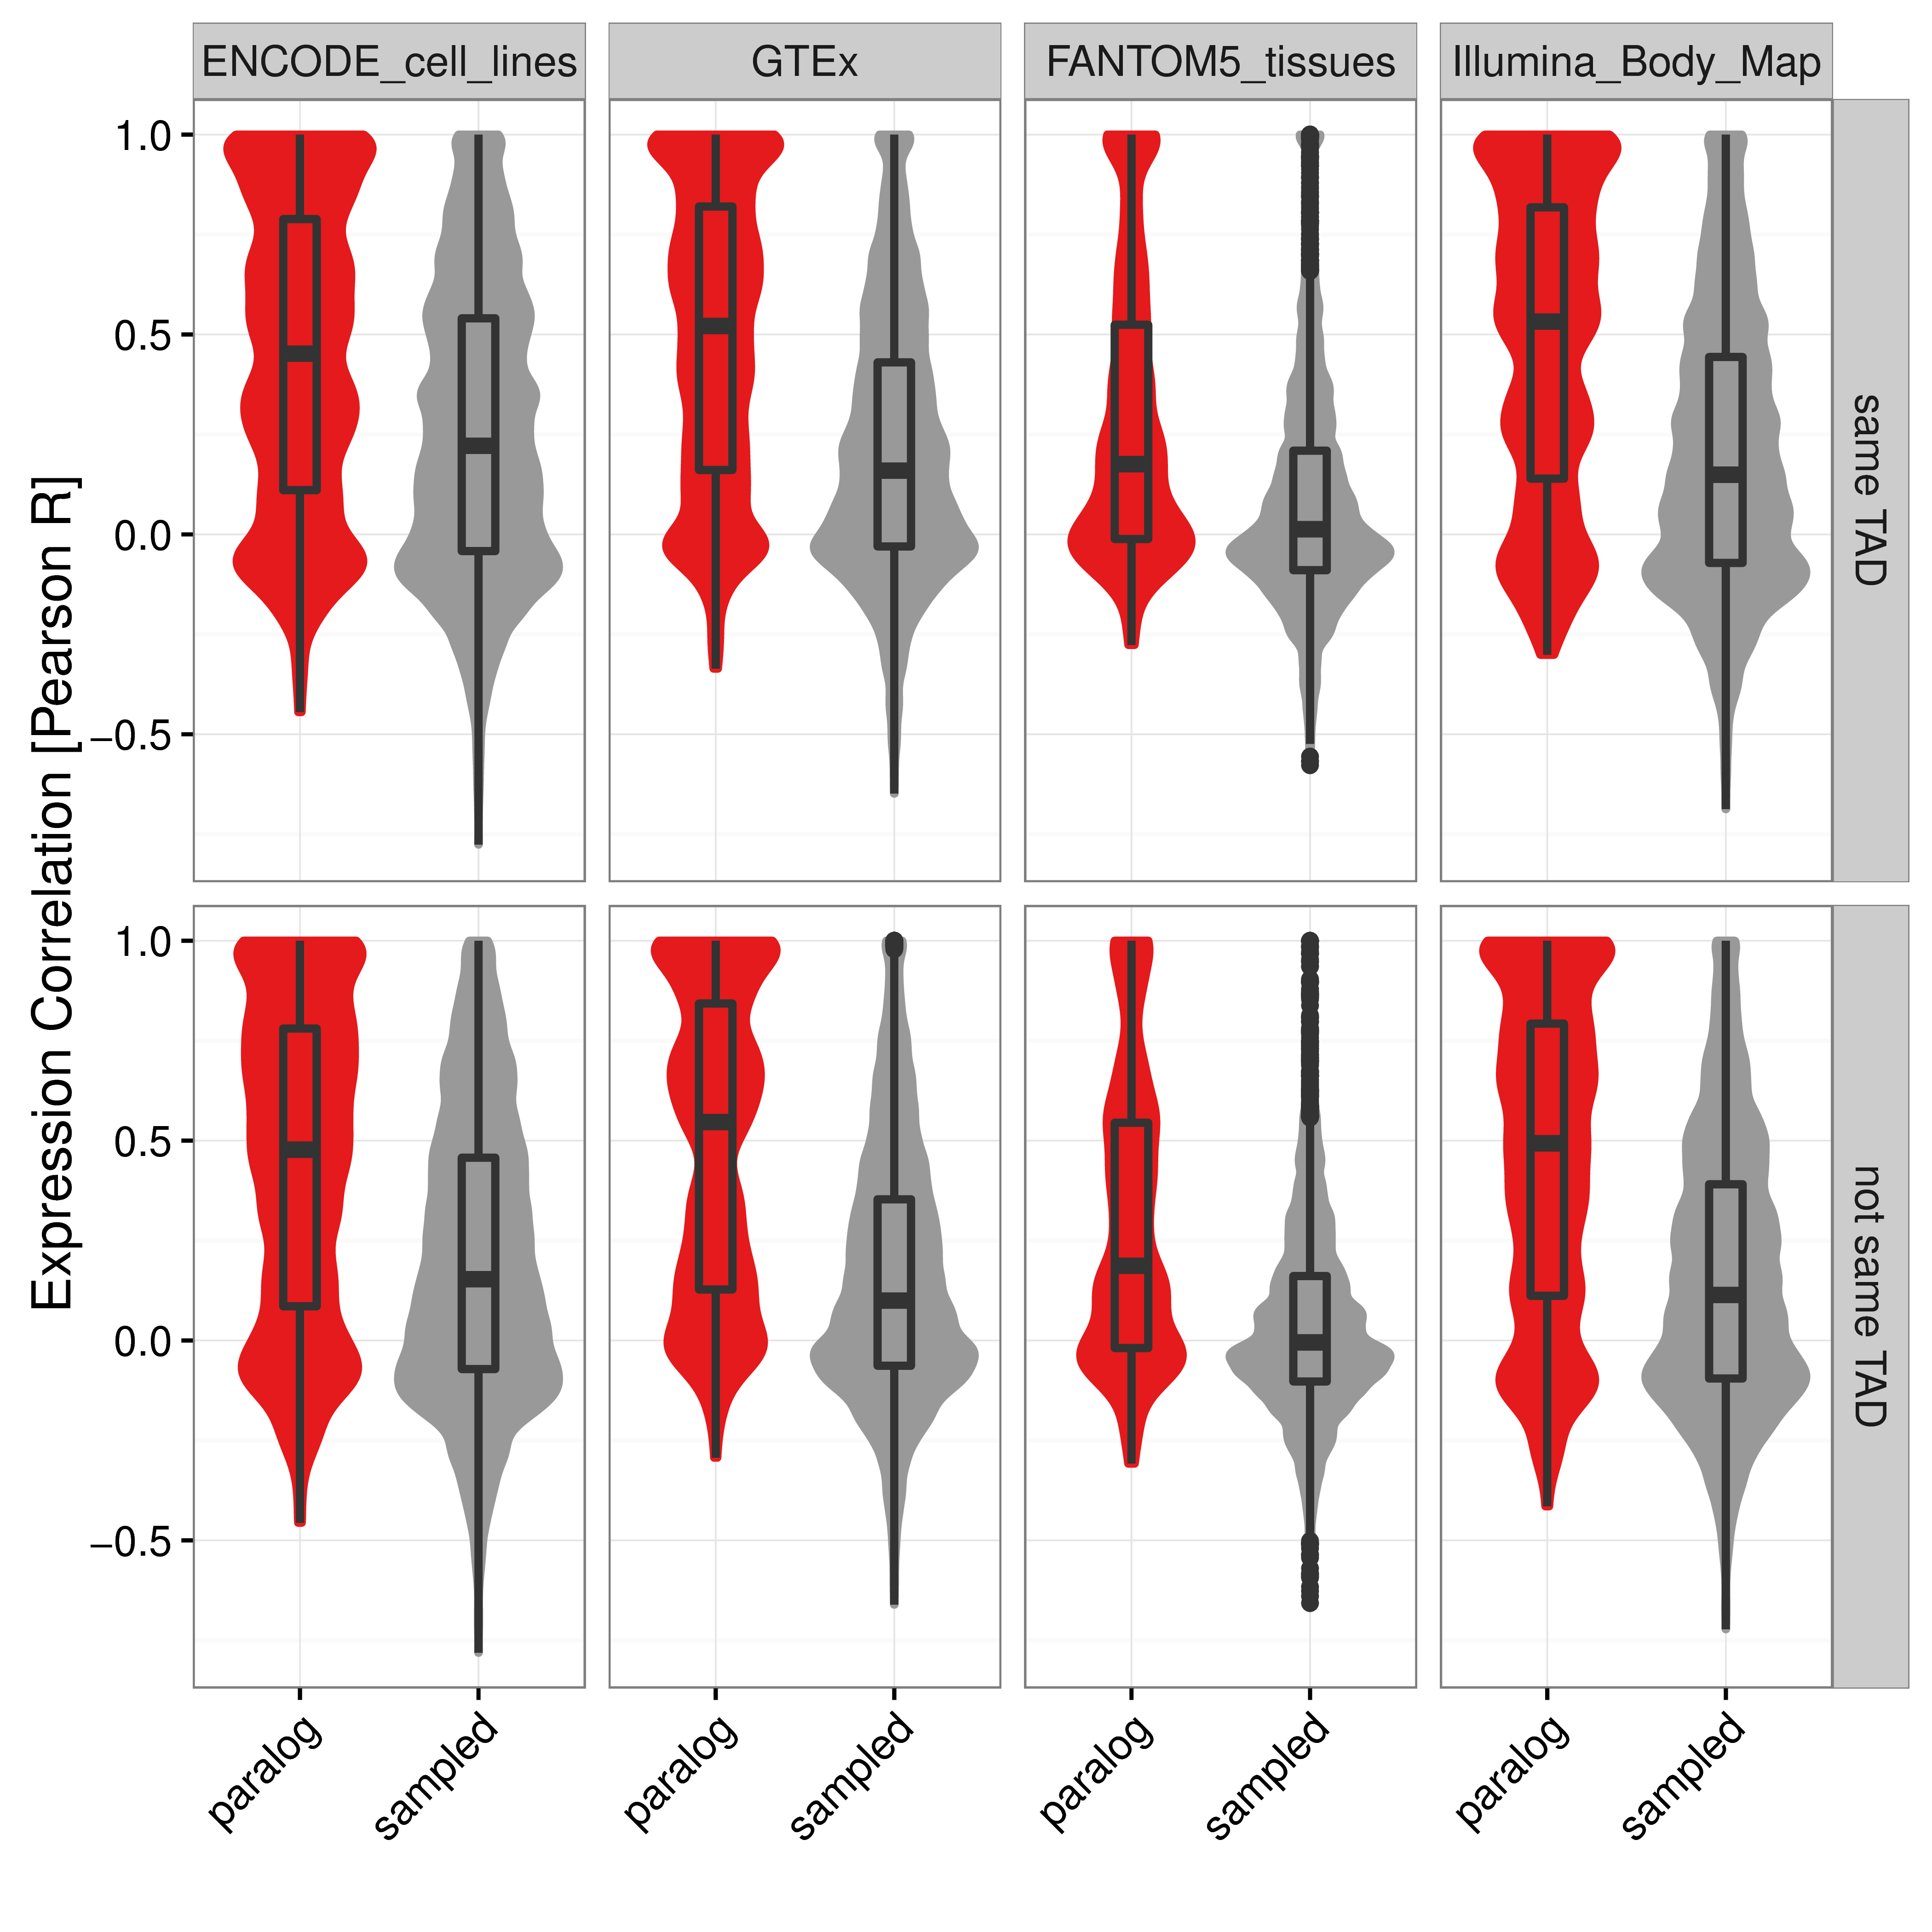
\includegraphics[width=0.5\linewidth]{figures/paralog/SI/figS10} 

}

\caption{Distribution of Pearson correlation coefficients of gene
expression values in four independent data sets between close paralog
gene pairs (red) and sampled control gene pairs (grey) separated for
gene pairs within the same IMR90 TAD (top) or not in the same TAD
(bottom). Boxes show 25th, 50th and 75th percent quantile of the data
and the filled areas indicate the density distribution.}\label{fig:ExpByTAD}
\end{figure}








\begin{figure}

{\centering 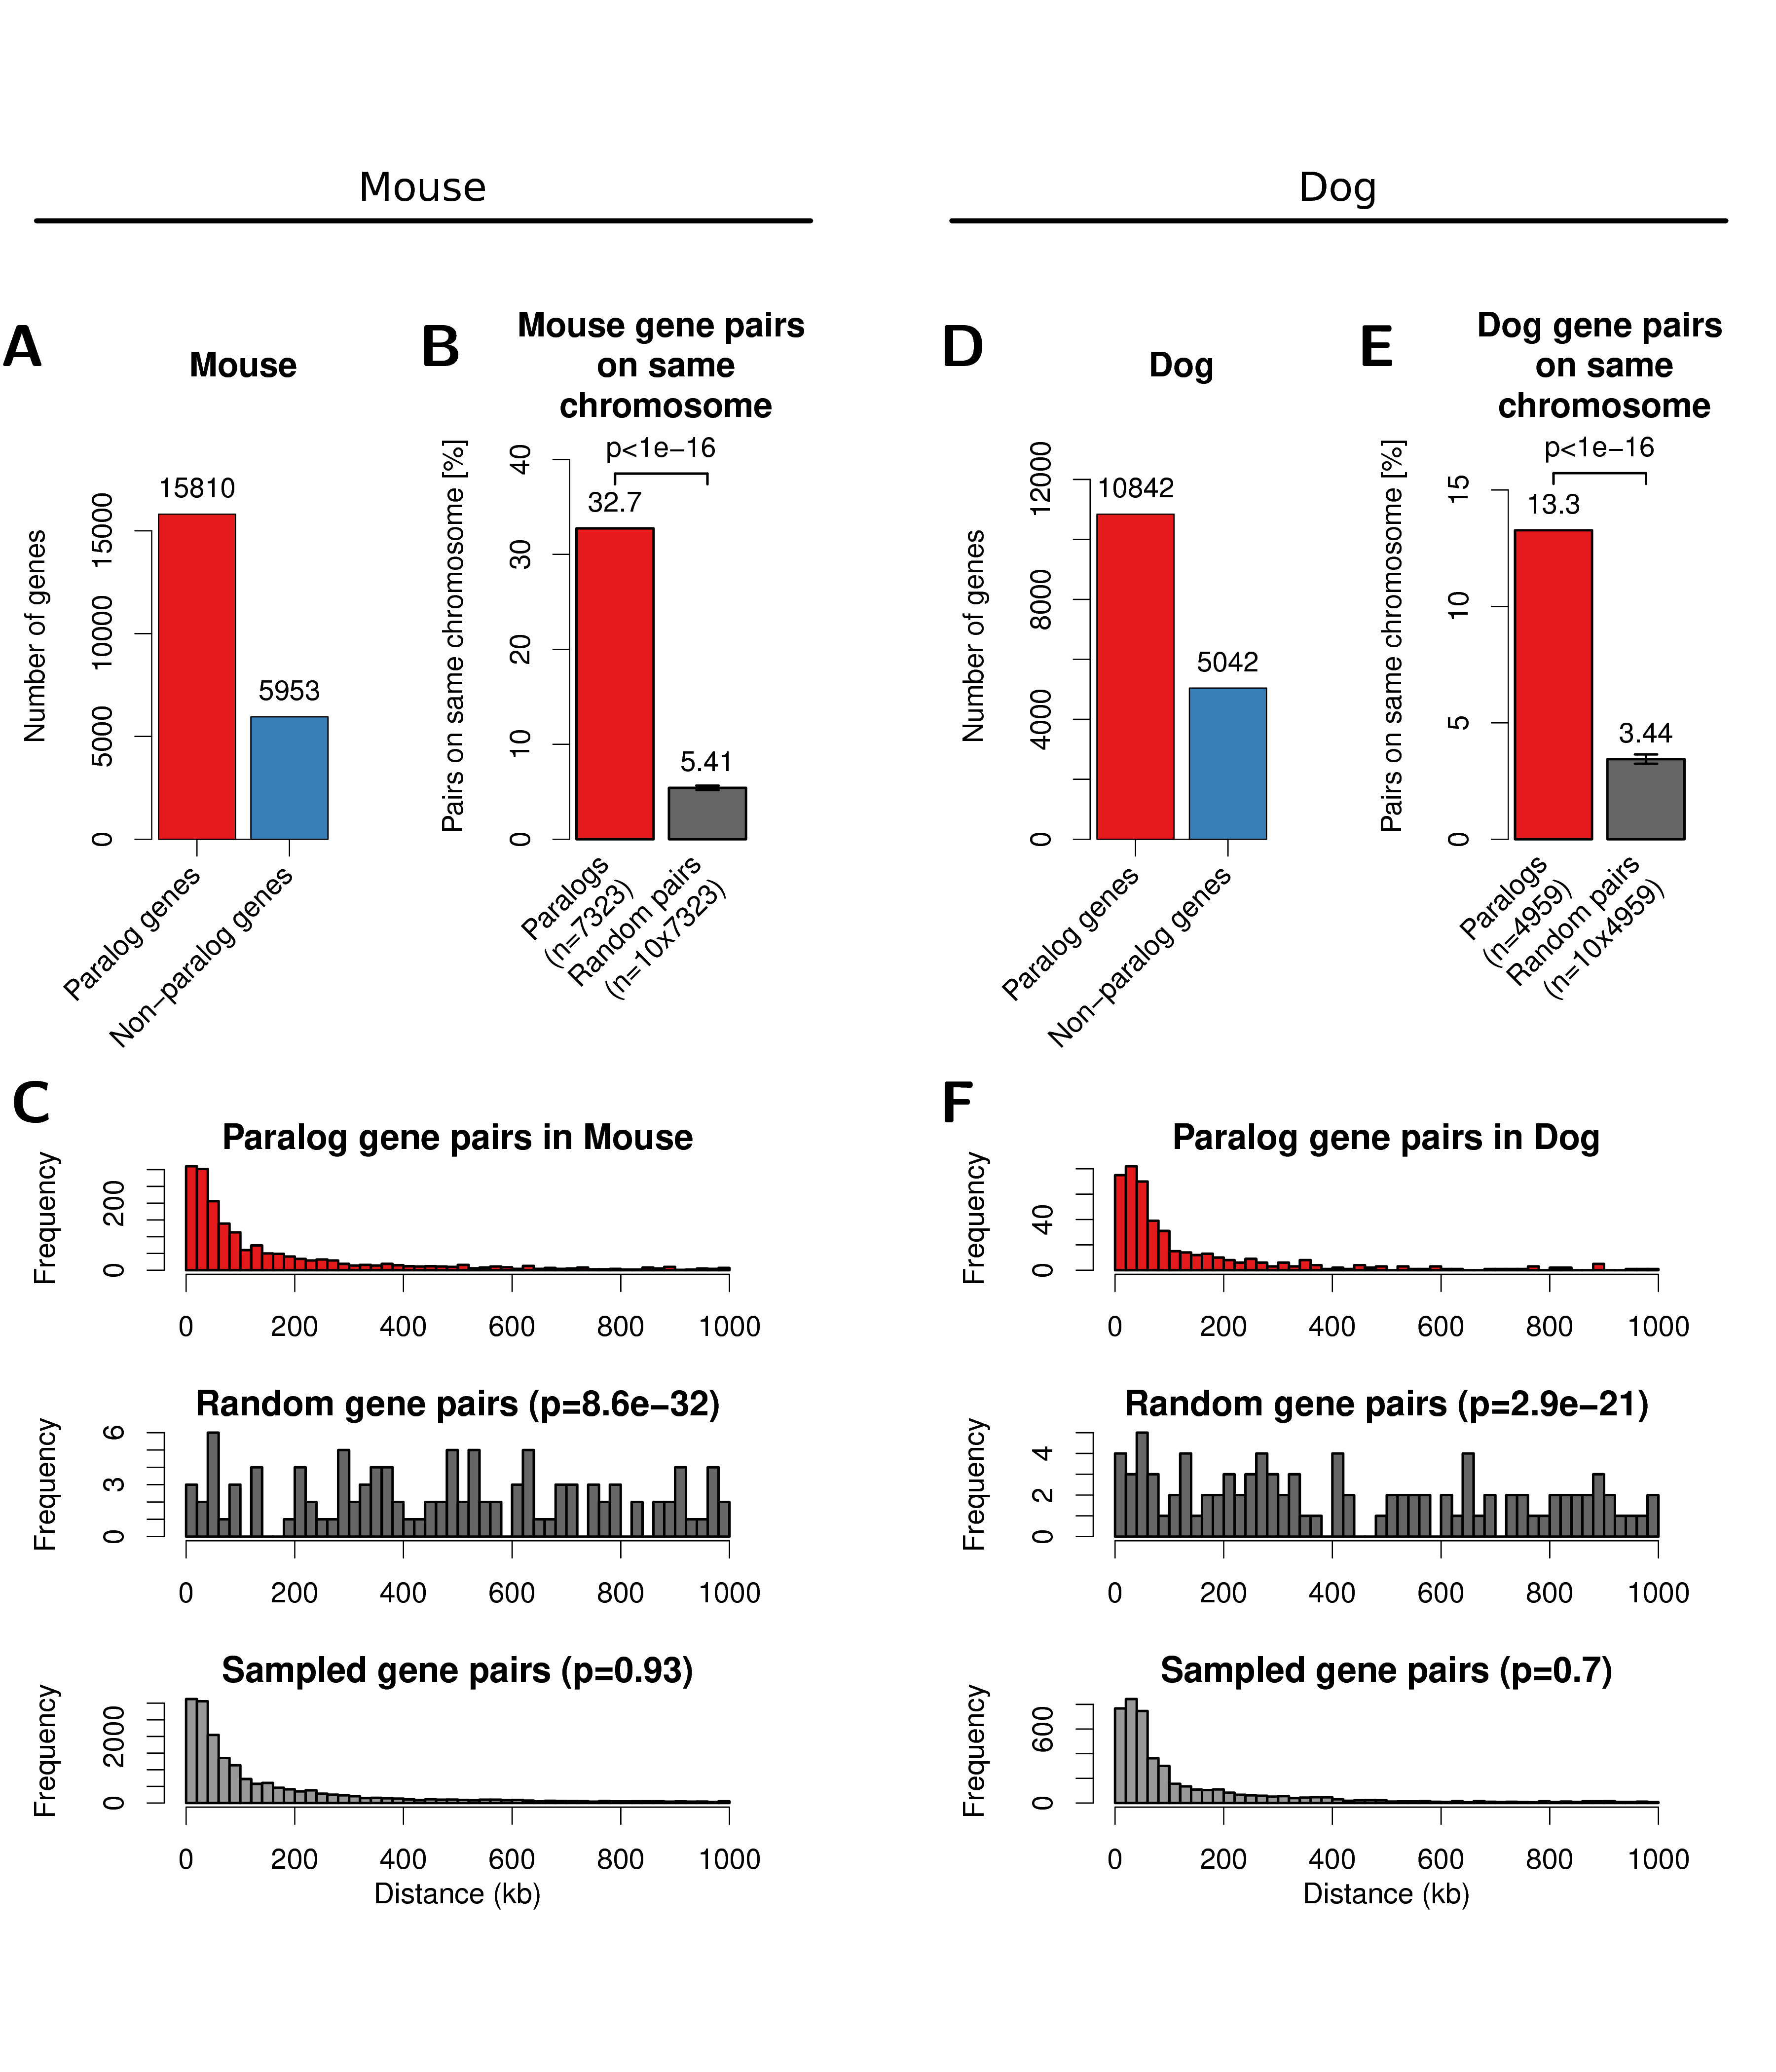
\includegraphics[width=0.5\linewidth]{figures/paralog/SI/figS11} 

}

\caption{Paralog gene pairs in mouse (left) and dog (right)
genome cluster on chromosome within short genomic distances.
\textbf{(A)} Number of genes with paralogs (red) and without (blue) in
mouse genomes. \textbf{(B)} Percent of filtered mouse paralog pairs on
the same chromosome (red) and random gene pairs on the same chromosome
(dark grey). Error-bars indicate standard deviation of 10 times
replicated randomizations. \textbf{(C)} Distribution of linear genomic
distances between mouse gene pairs for filtered paralog genes (top,
red), random genes (center, dark grey) and sampled gene pairs (bottom,
grey). \textbf{(D, E, F)} show the same data for the dog genome as
figures A, B, C, respectively.}\label{fig:paralogsSpecies}
\end{figure}













\begin{figure}

{\centering 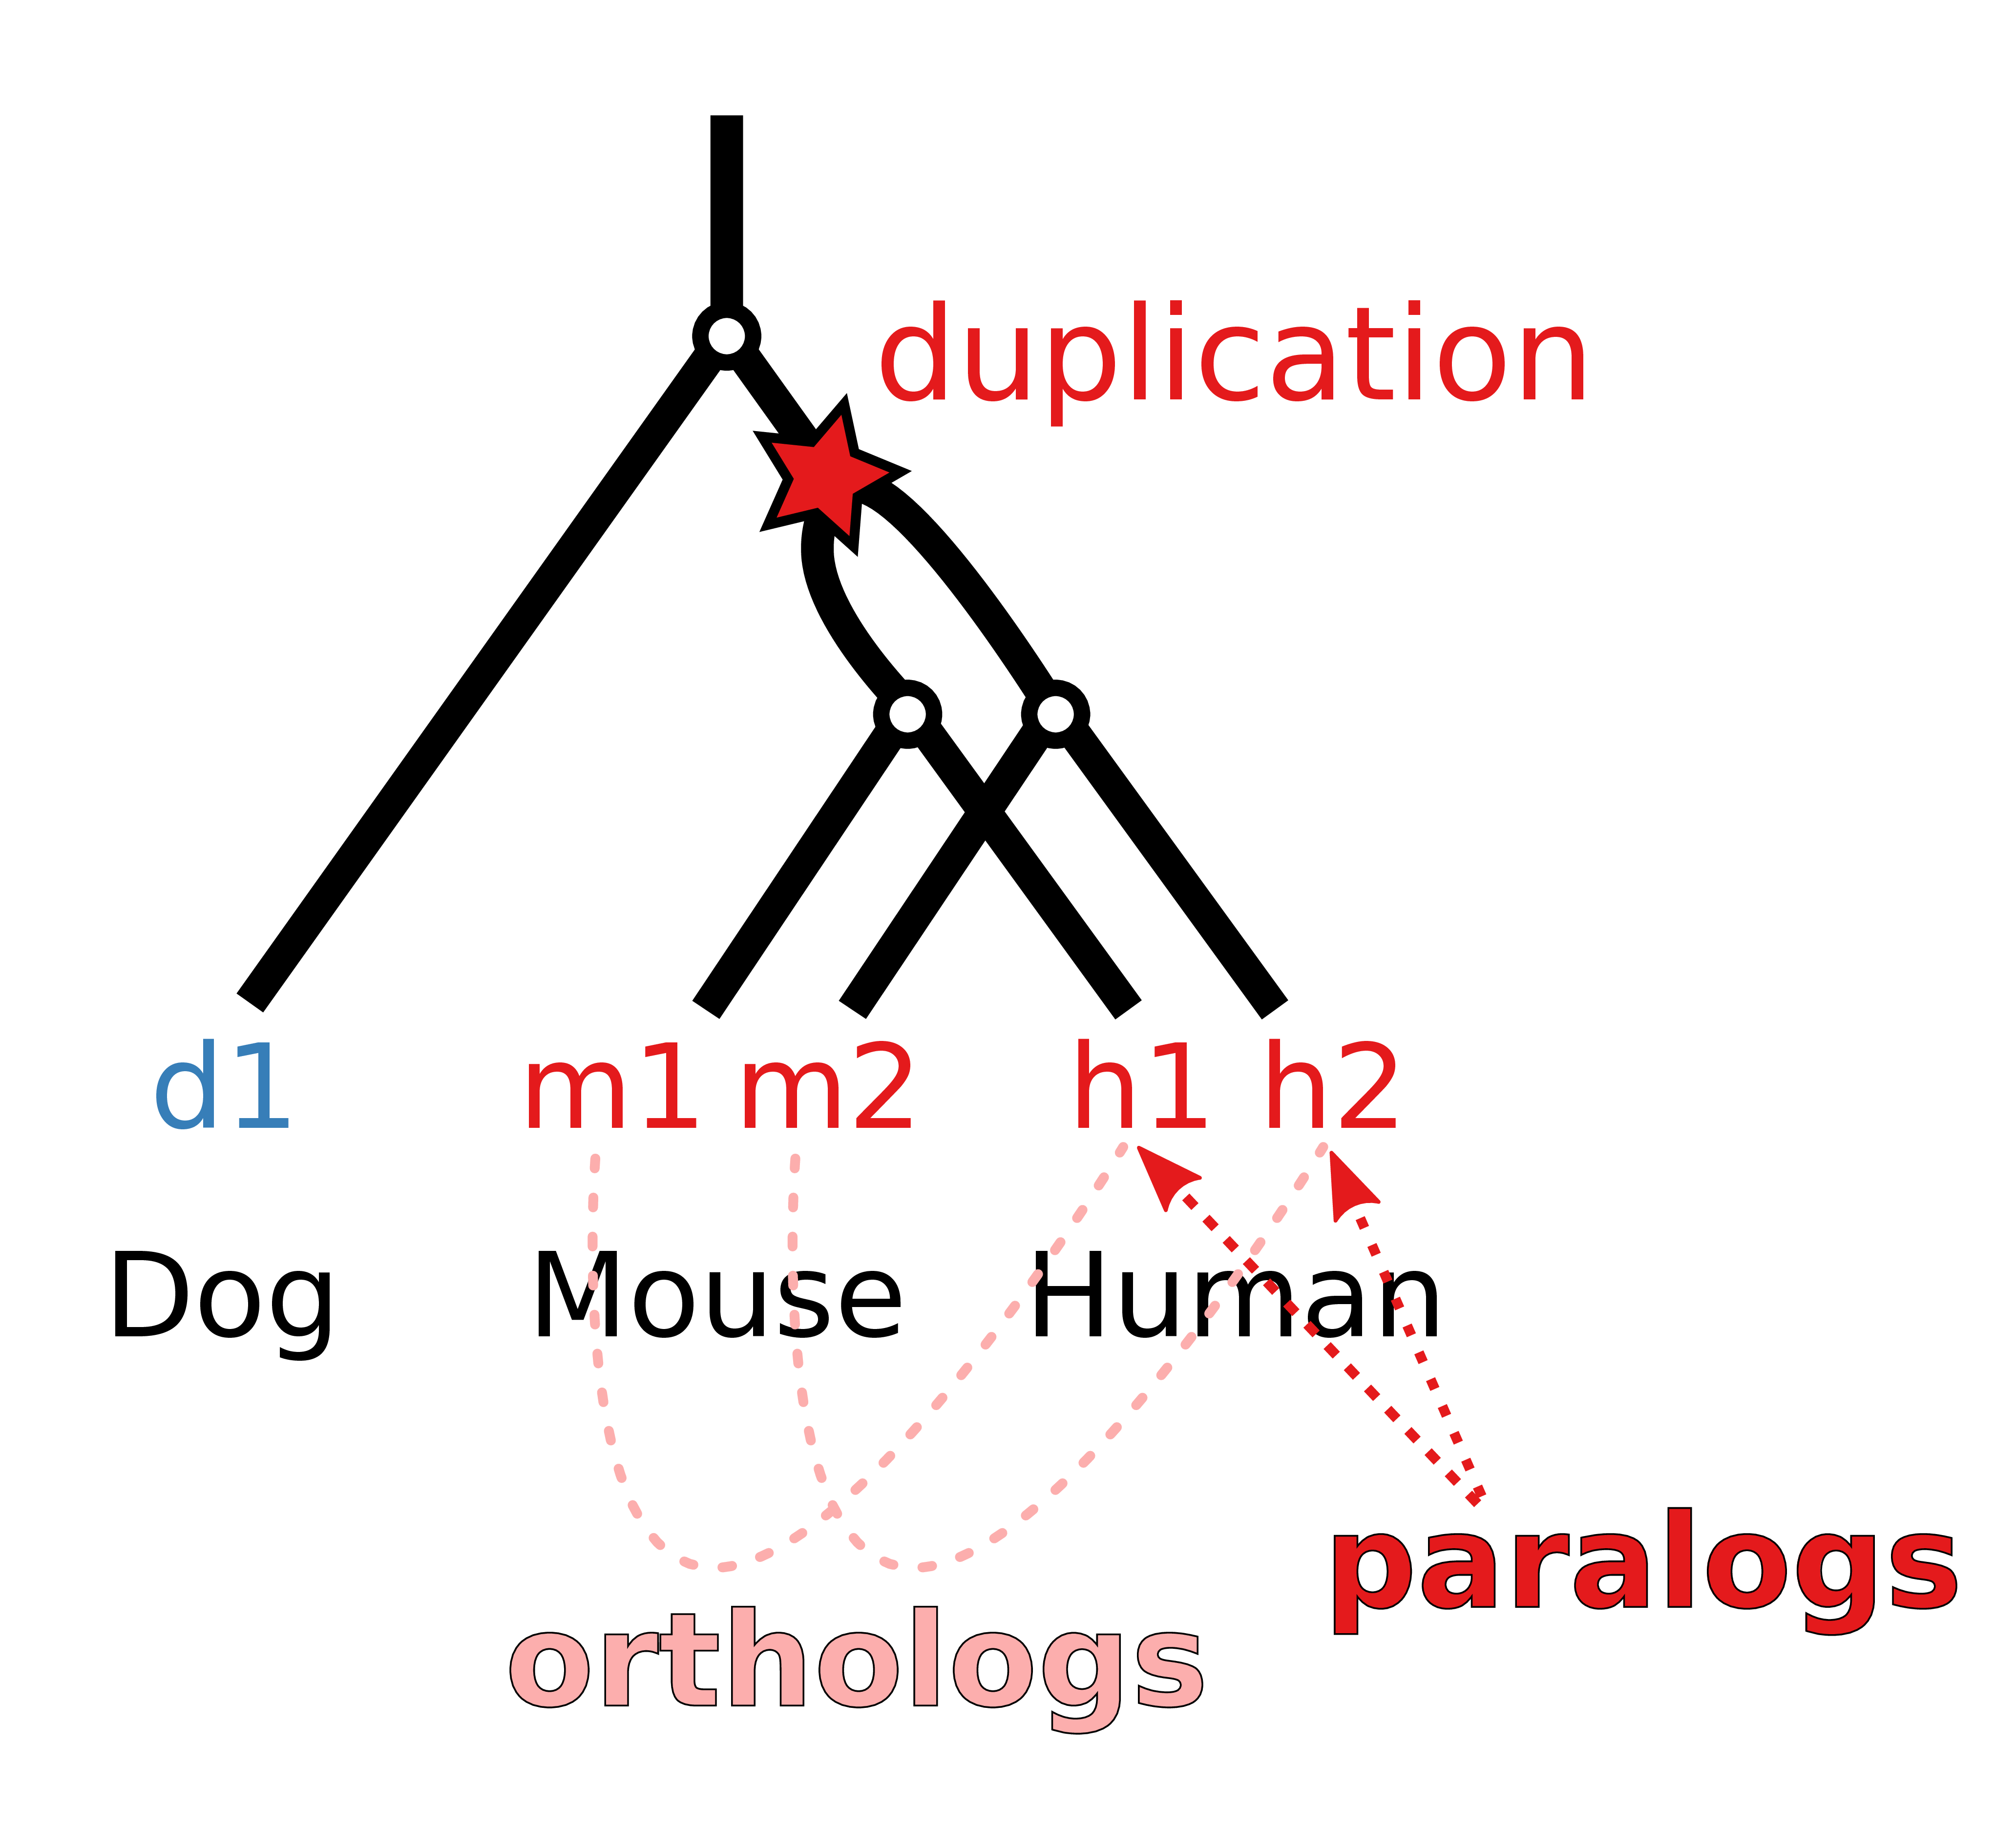
\includegraphics[width=0.5\linewidth]{figures/paralog/SI/figS12} 

}

\caption{Phylogenetic gene tree model of a gene that is
duplicated before the separation of mouse and human and consequently
leads to two paralogs in mouse and human that are one-to-one orthologs
to each other and a single ortholog in the dog genome that cannot be
assigned uniquely to a human gene.}\label{fig:orthologModel}
\end{figure}







\begin{figure}

{\centering 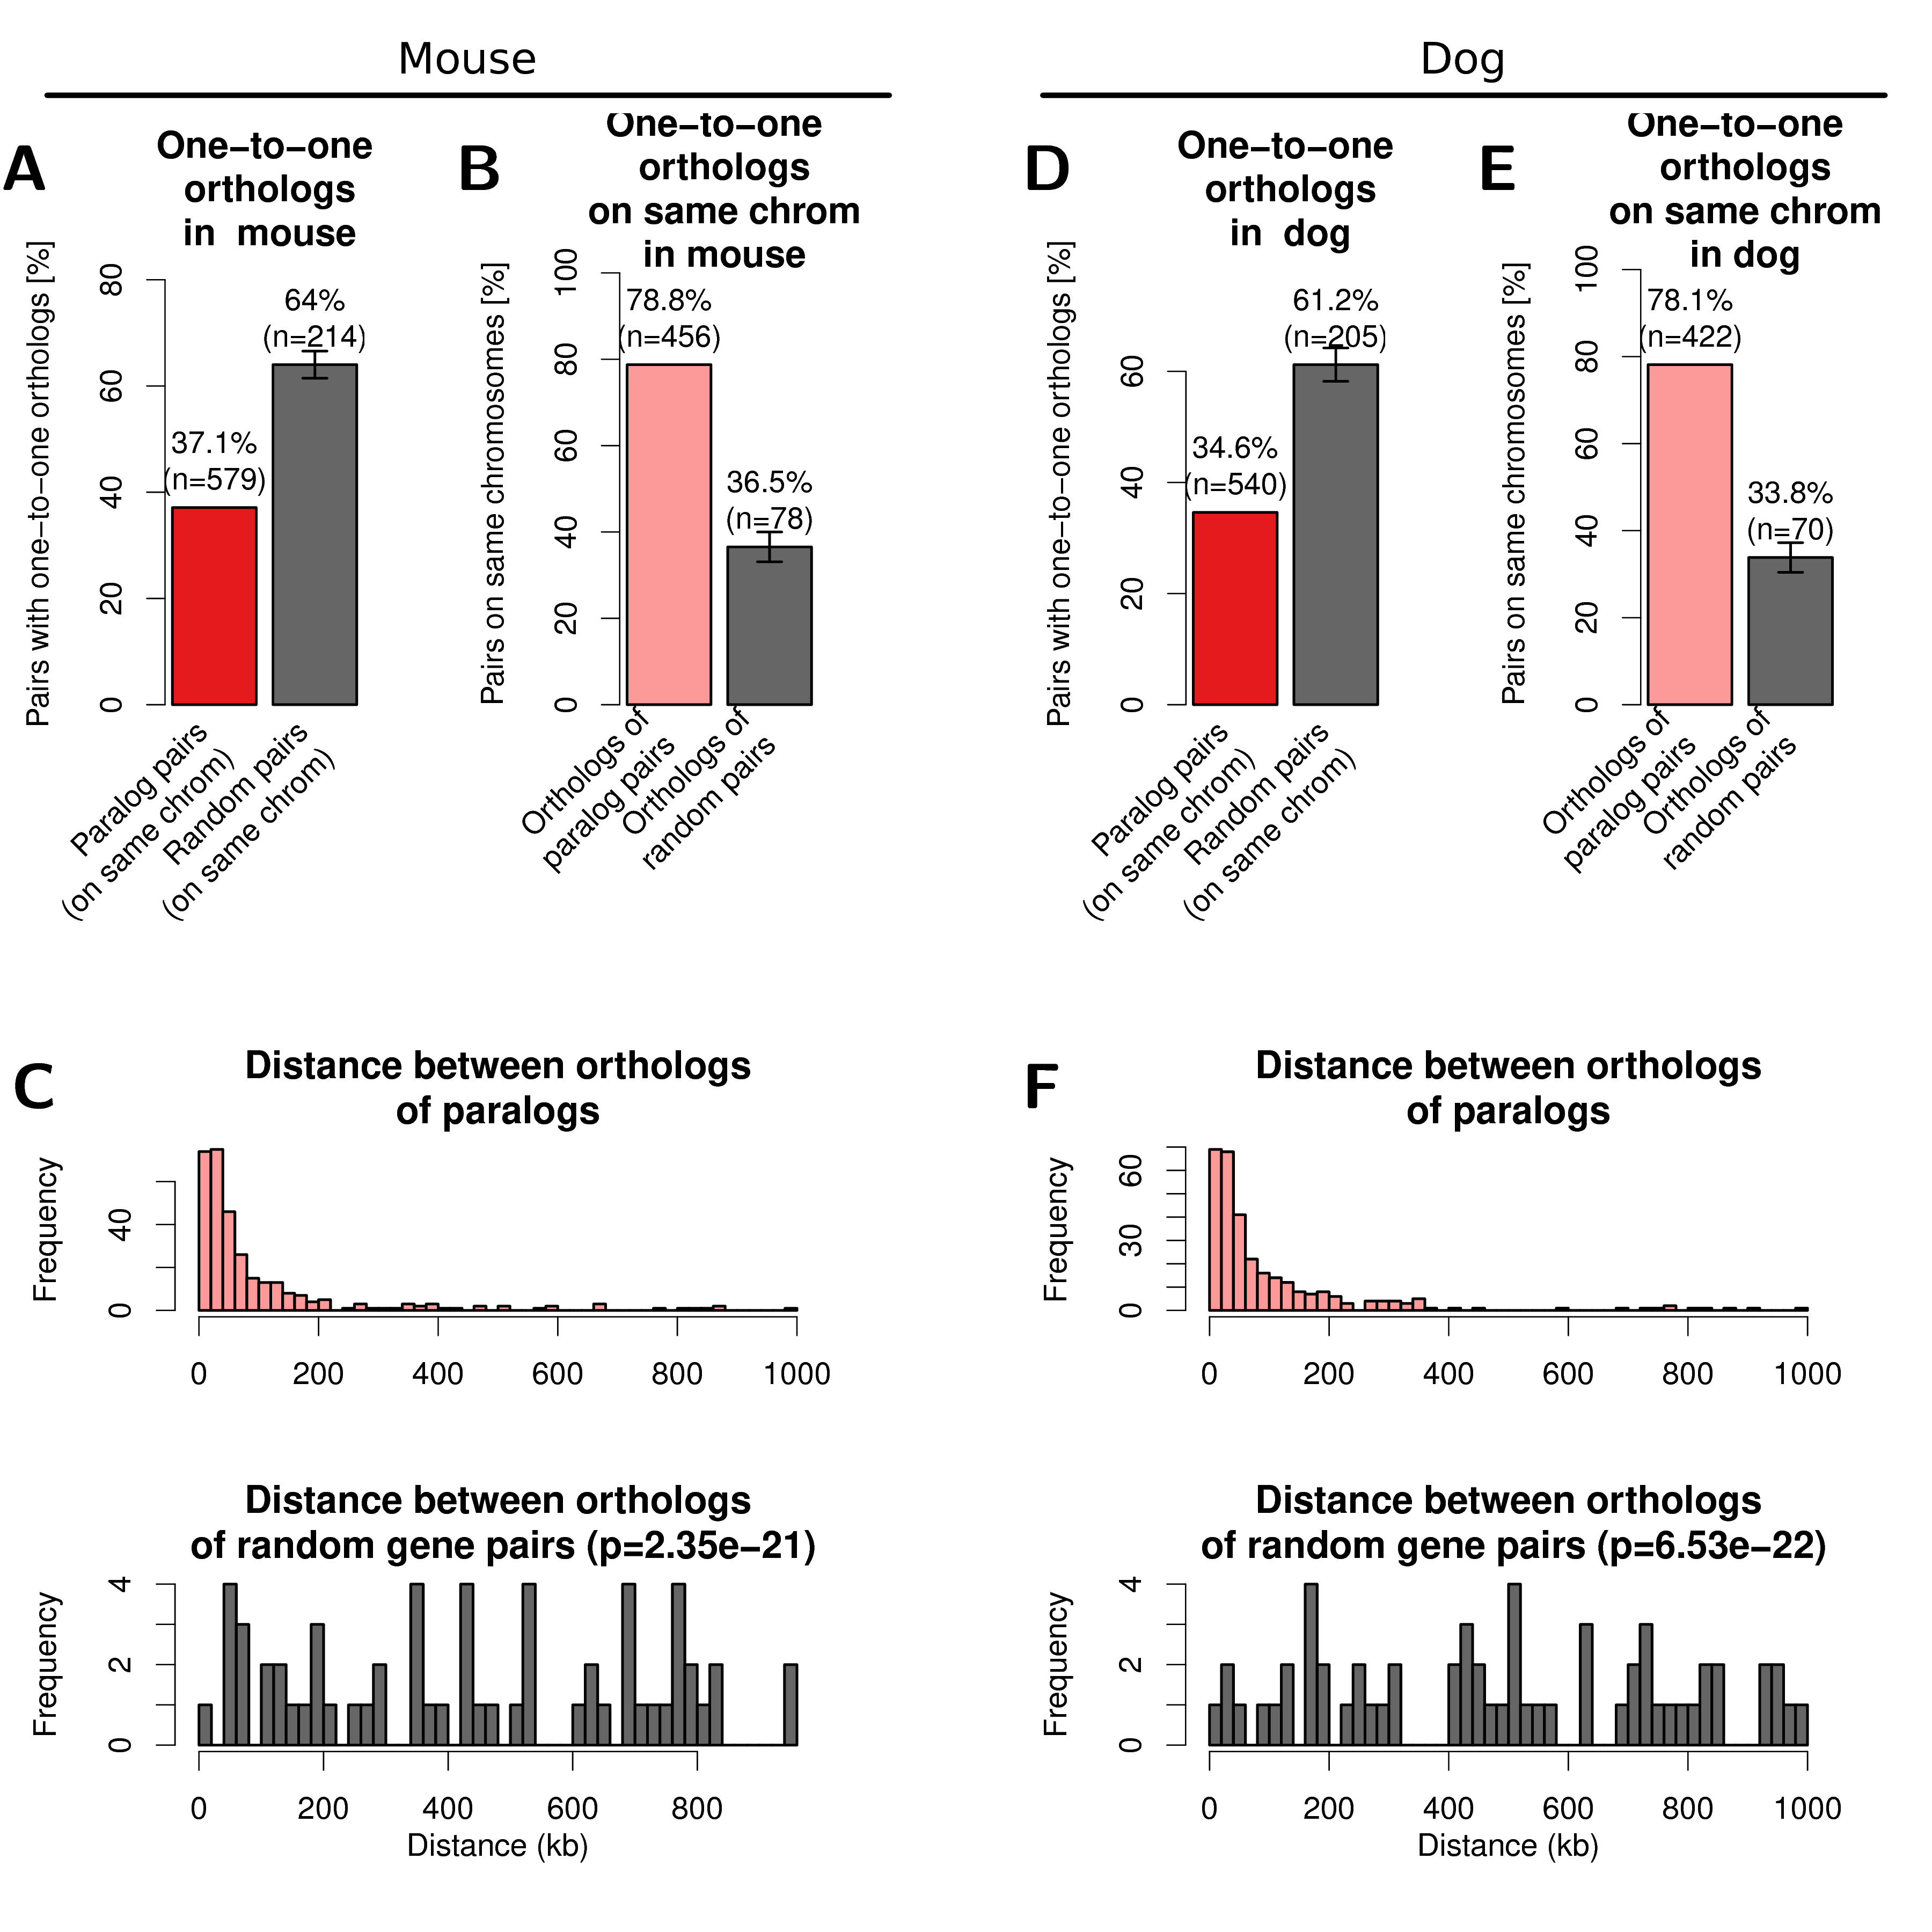
\includegraphics[width=0.5\linewidth]{figures/paralog/SI/figS13} 

}

\caption{One-to-one orthologs of human paralogs in mouse
(left) and dog (right) genome. \textbf{(A)} Percent of filtered human
paralog pairs with one-to-one orthologs for both genes in mouse genome
compared to random genes. \textbf{(B)} Percent of one-to-one orthologs
on the same chromosome in the mouse genome (light red) and one-to-one
orthologs of random human gene pairs on the same chromosome (dark grey).
Error-bars indicate standard deviation of 10 times replicated
randomizations. \textbf{(C)} Distribution of linear genomic distances
between gene pairs for mouse one-to-one orthologs of human paralog gene
pairs (top, light red) and one-to-one orthologs of random human gene
pairs (bottom, dark grey). \textbf{(D, E, F)} show the same data for the
dog genome as figures A, B, C, respectively.}\label{fig:orthologsSpecies}
\end{figure}














\begin{figure}

{\centering 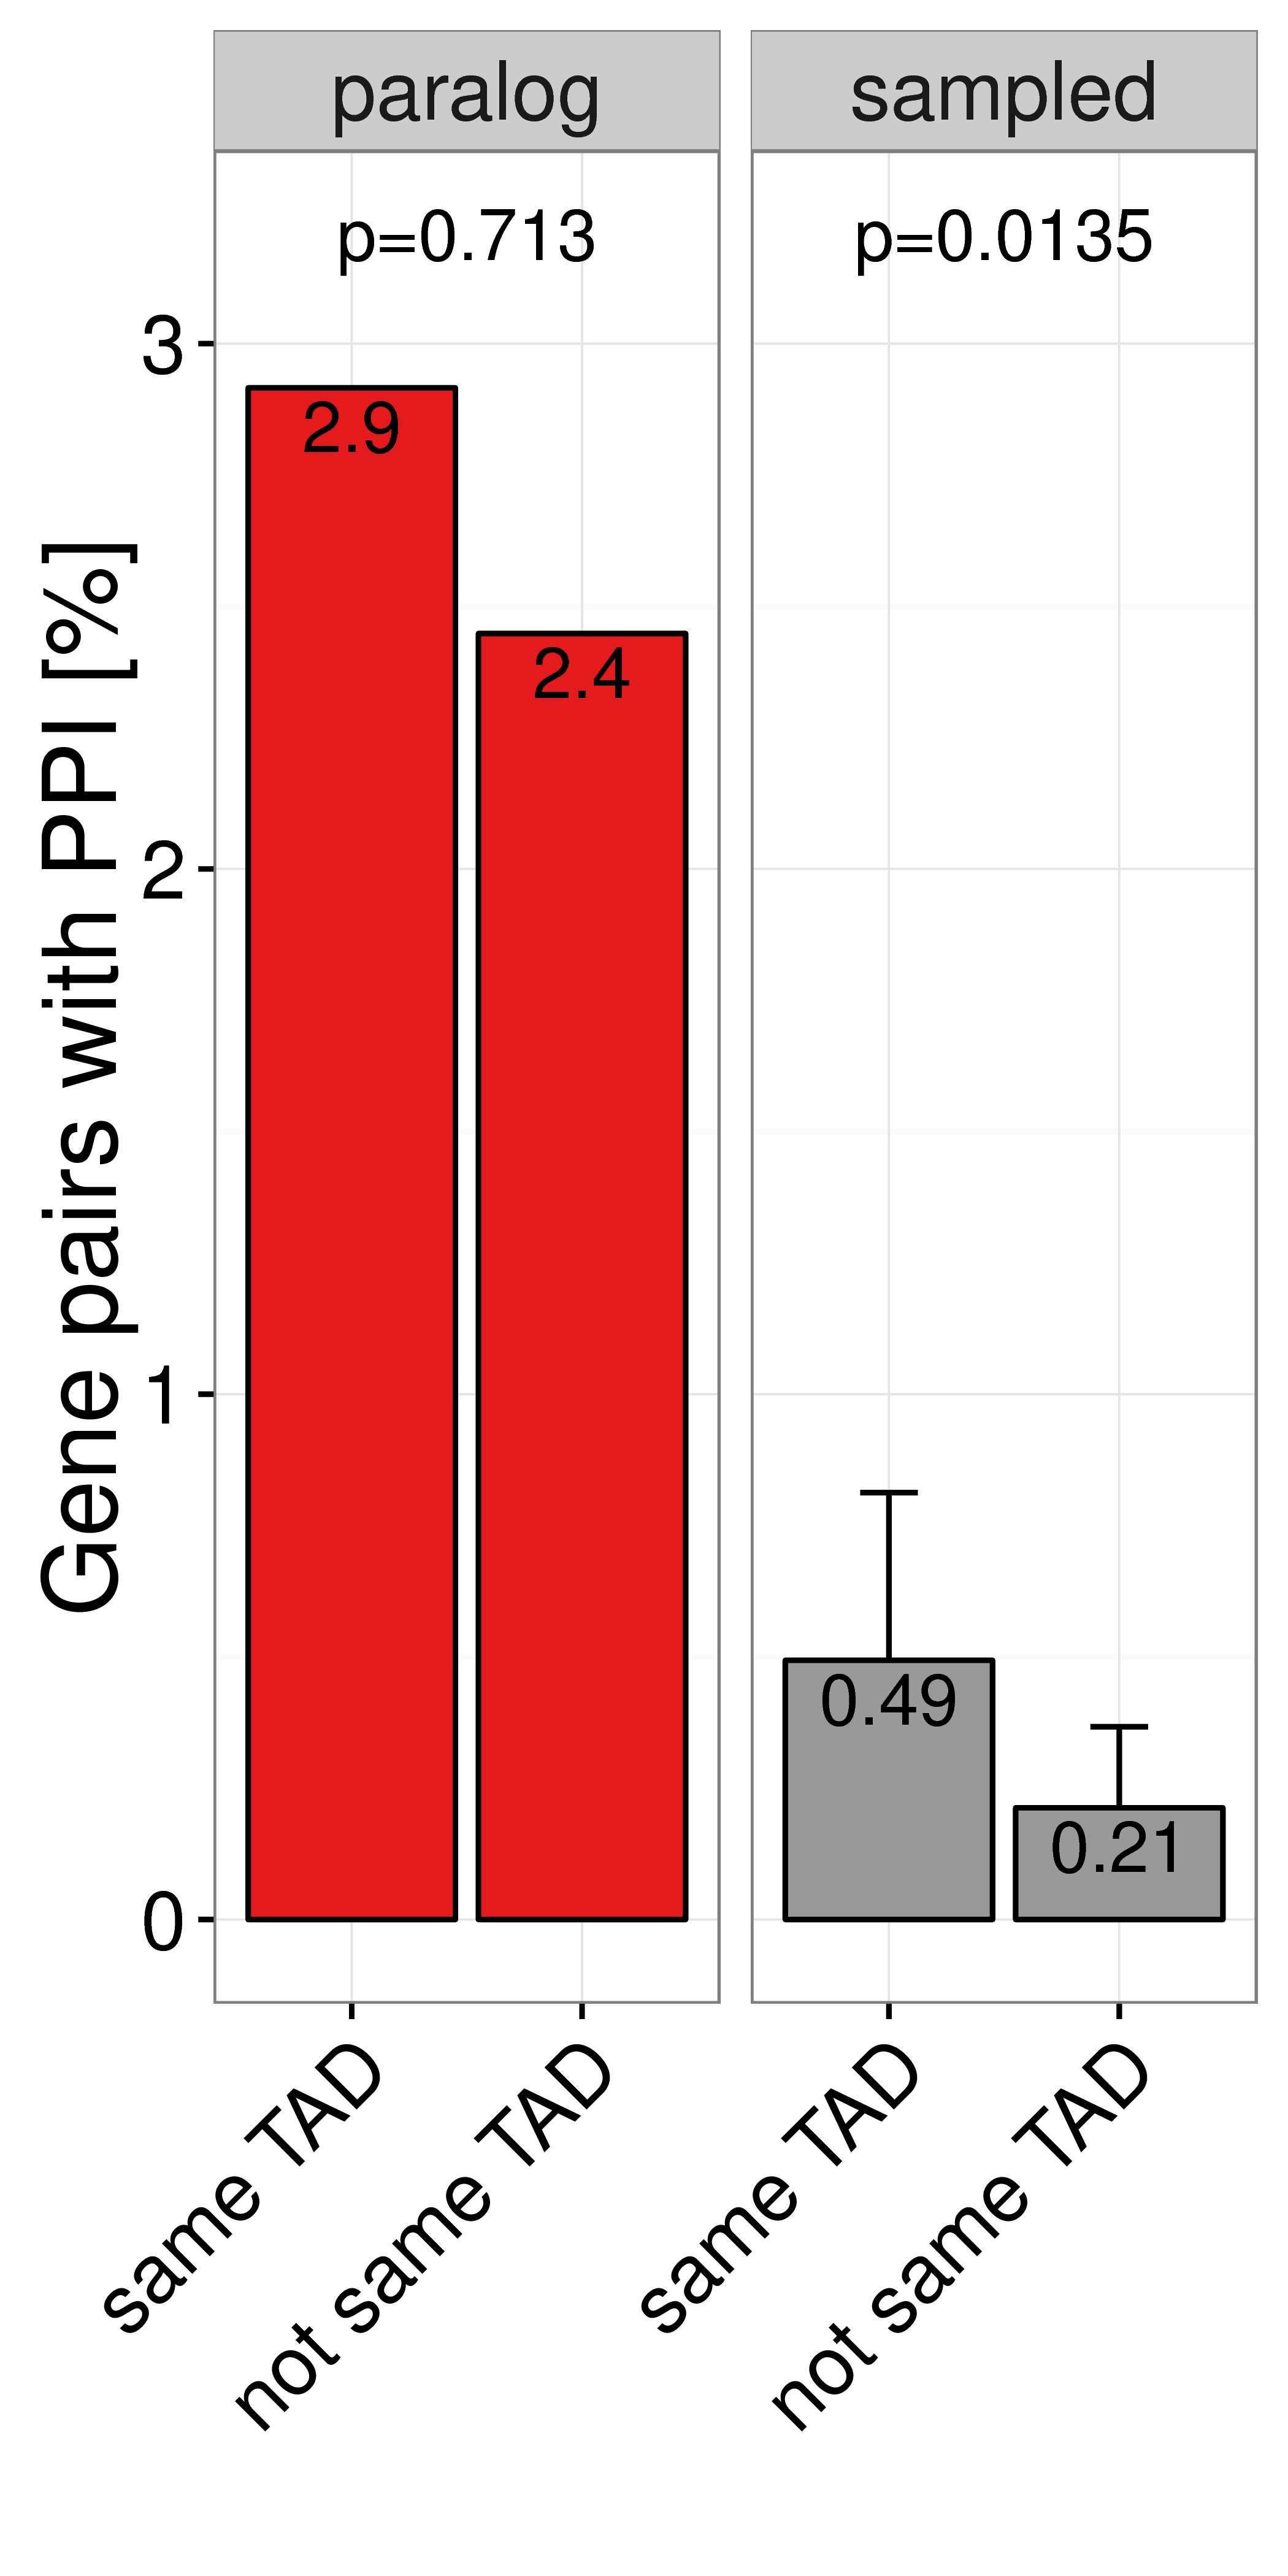
\includegraphics[width=0.5\linewidth]{figures/paralog/SI/figS14} 

}

\caption{Percent of close paralogs (red) and sampled (grey) gene pairs
in the same IMR90 TAD (left bar) or not same TAD (right bar) that have a
direct protein protein interaction (PPI) with each other in the HIPPIE
database \citep{Schaefer2012}.}\label{fig:PPI}
\end{figure}






\chapter{Supplementary Data: Evolutionary stability of topologically
associating domains is associated with conserved gene
regulation}\label{supplementary-data-evolutionary-stability-of-topologically-associating-domains-is-associated-with-conserved-gene-regulation}

\hypertarget{TadEvoSupTab}{\section{Supplementary
Tables}\label{TadEvoSupTab}}

\textbf{Table S1} \textbf{Matching tissues and samples with CAGE
expression data in human and mouse.}
\url{https://www.biorxiv.org/highwire/filestream/70793/field_highwire_adjunct_files/2/231431-3.tsv}

\textbf{Table S2} \textbf{Ortholog genes in human and mouse with gene
expression correlation across tissues.}
\url{https://www.biorxiv.org/highwire/filestream/70793/field_highwire_adjunct_files/3/231431-4.tsv}

\section{Supplementary Figures}\label{supplementary-figures}

\begin{figure}

{\centering 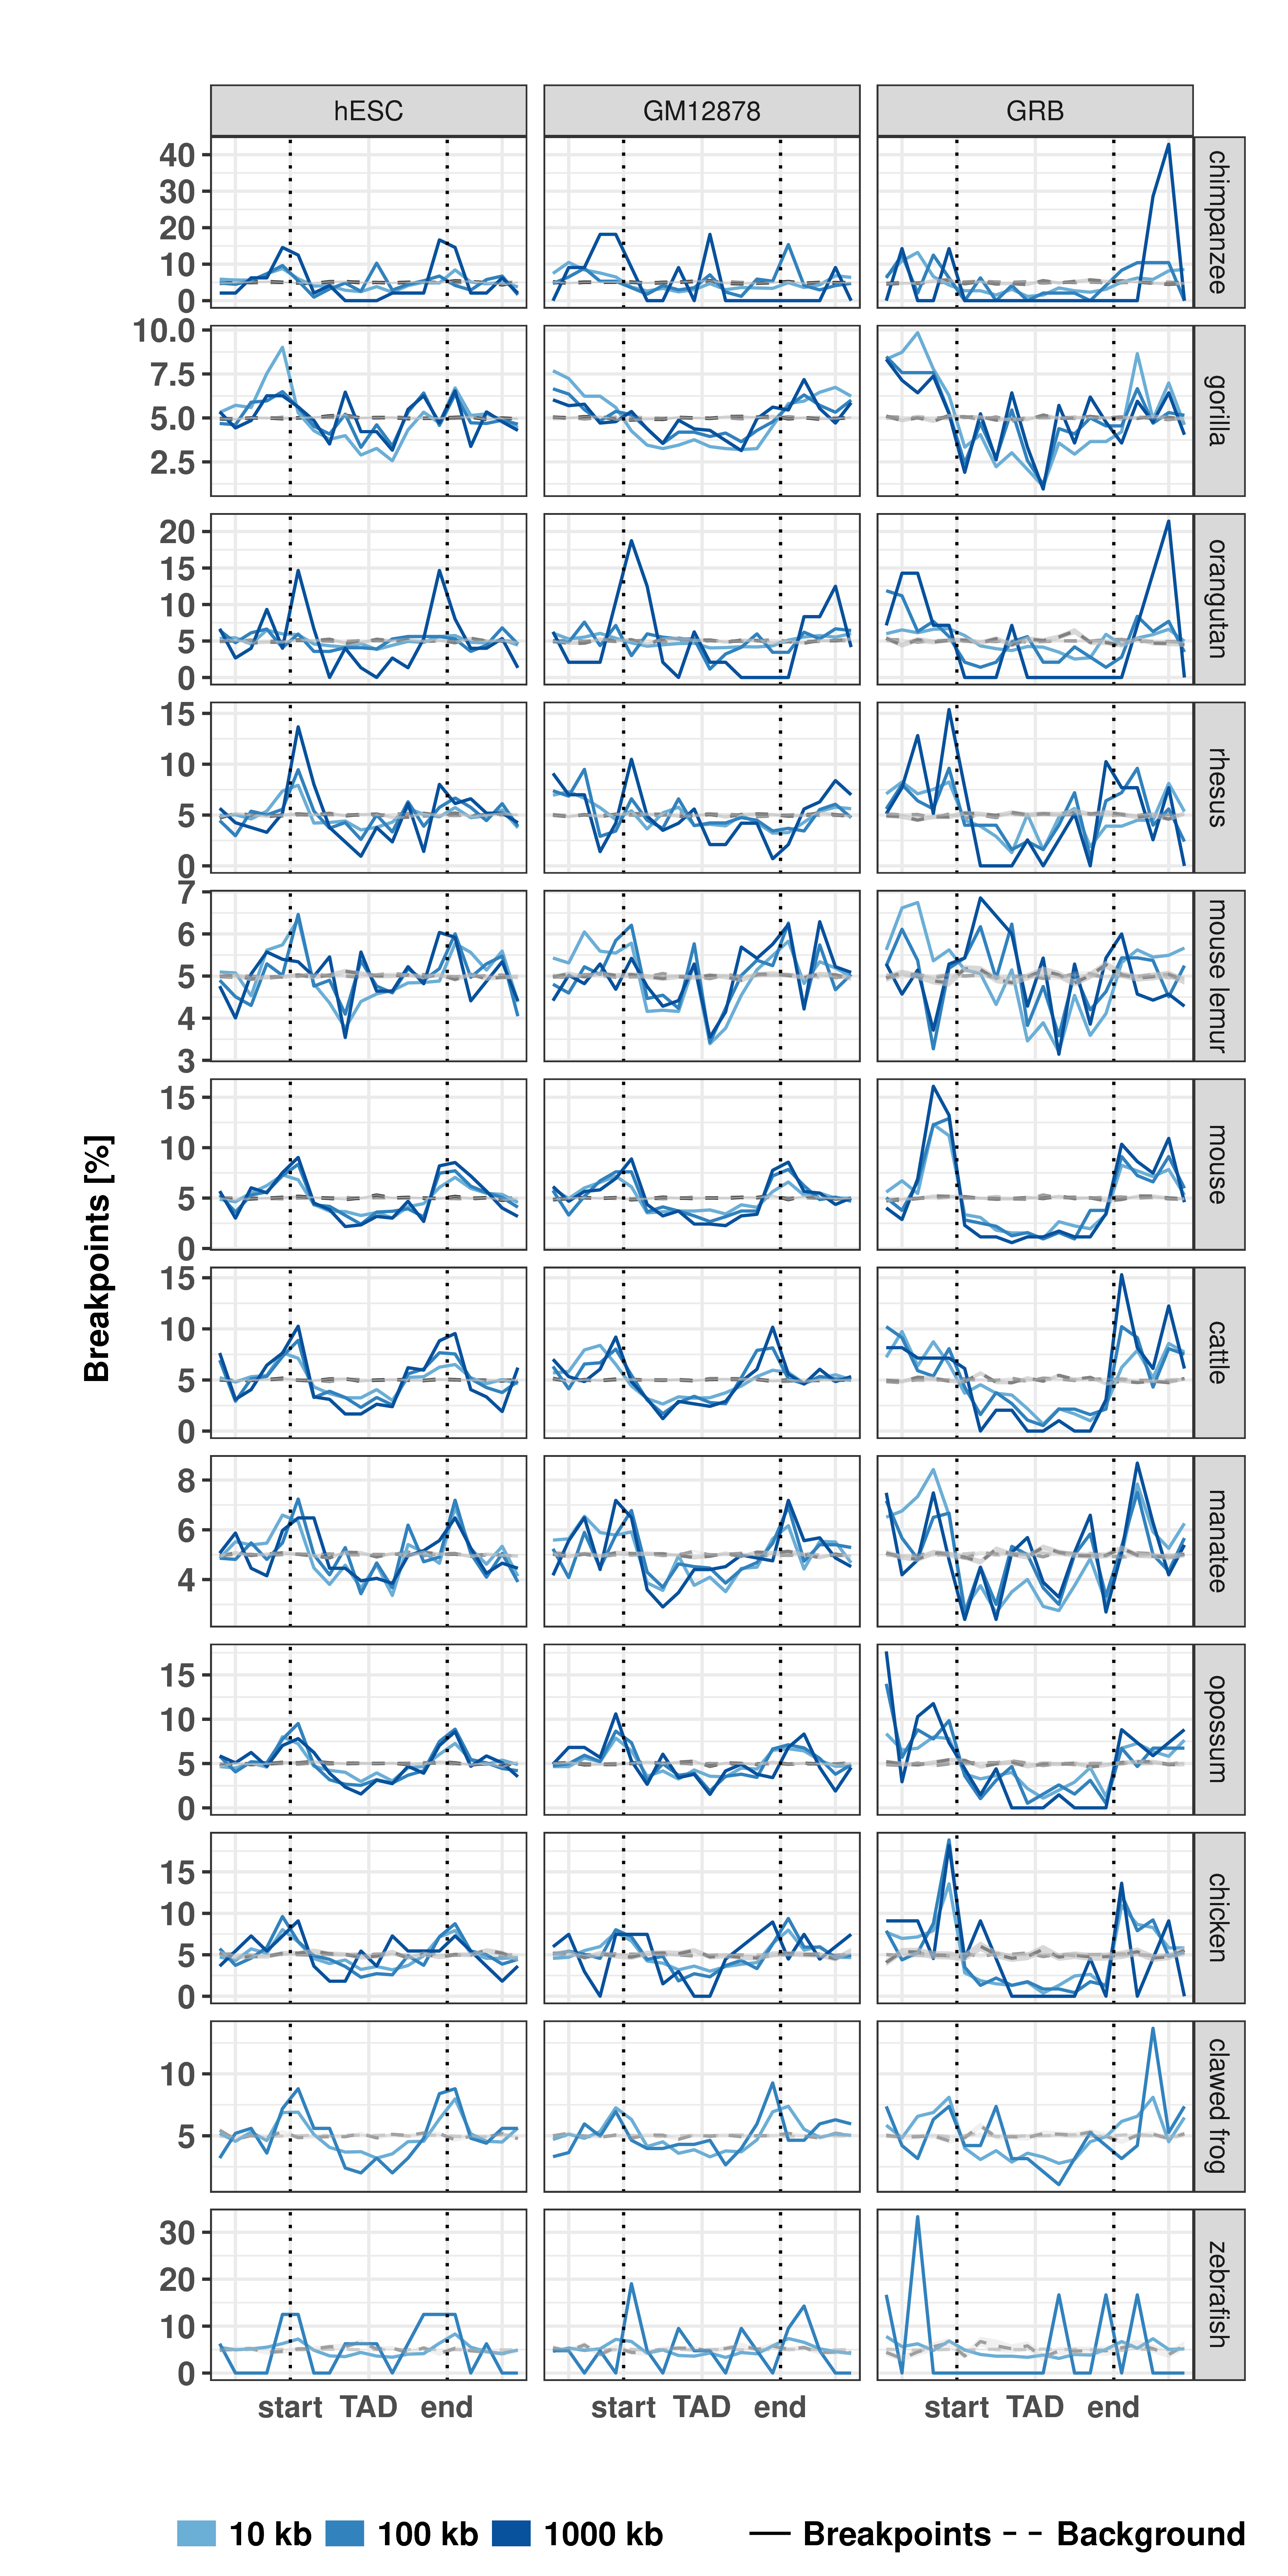
\includegraphics[width=0.8\linewidth]{figures/TAD_evolution/fig_S1_v01} 

}

\caption{\textbf{Distribution of evolutionary rearrangement
breakpoints between human and 12 vertebrate genomes around domains.}
Relative breakpoint numbers from human and different species (horizontal
panels) around hESC TADs (left), GM12878 contact domains (center), and
GRBs (left). Blue color scale represents breakpoints from different
fill-size thresholds. Dotted lines in gray show simulated background
controls of randomly placed breakpoints.}\label{fig:TadEvoS1}
\end{figure}









\begin{figure}

{\centering 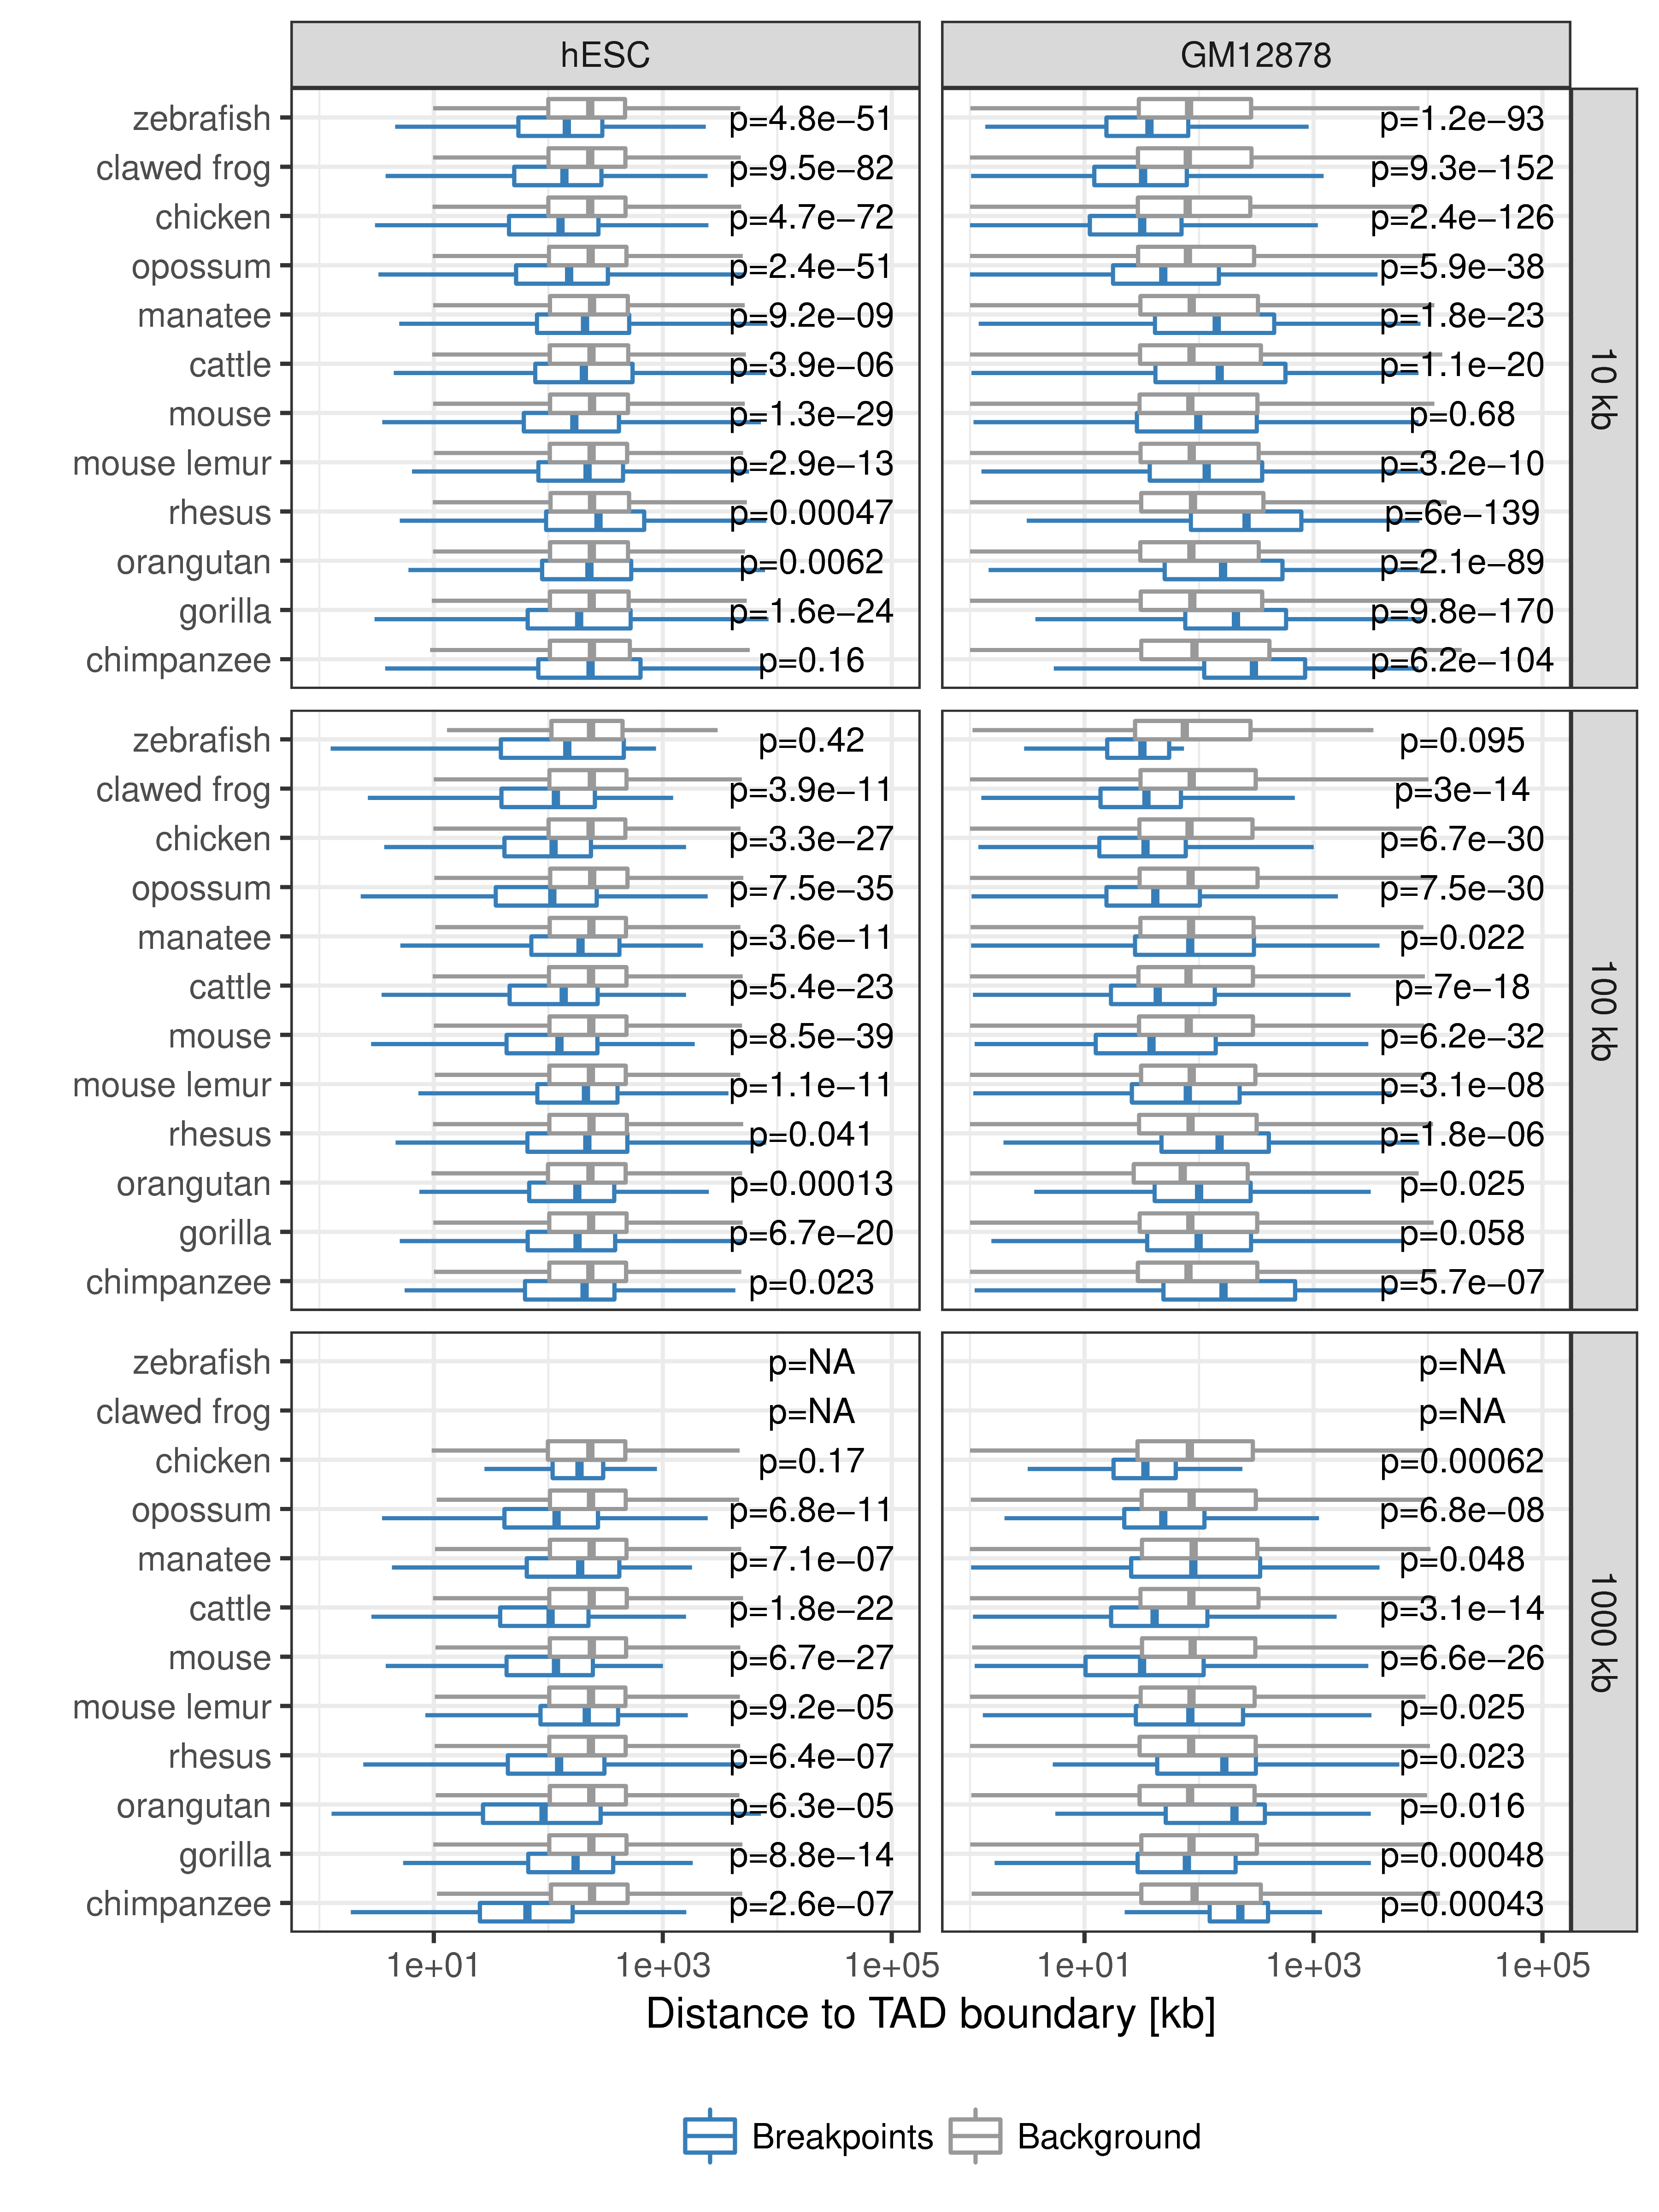
\includegraphics[width=0.8\linewidth]{figures/TAD_evolution/fig_S2_v01} 

}

\caption{\textbf{Distance between rearrangement breakpoints and
random controls to closest TAD boundary.} For each species (y-axis) and
fill size threshold (vertical panels) the distances from all identified
rearrangement breakpoints to its closest TAD boundary (x-axis) are
compared between actual rearrangements (blue) and 100 times randomized
background controls (gray). The left panel shows distances to next hESC
TAD boundary and the right panel distances to closest GM12878 contact
domain boundary. P-values according to Wilcoxon's rank-sum test.}\label{fig:TadEvoS2}
\end{figure}










\bibliography{bib/book.bib,bib/packages.bib,bib/PhD.bib}



% \bibliography{book.bib, packages.bib, PhD.bib}

\end{document}
